% % % % % % % % % % % % % % % % % % % %% % % % % % % % % %% % % % % % % % % %
% Cours Électromagnétisme
% Version: 24 Novembre 2020
% % % % % % % % % % % % % % % % % % % %% % % % % % % % % %% % % % % % % % % %
\documentclass[12pt]{book}
\usepackage{teach}
\usepackage[utf8]{inputenc}
\usepackage[T1]{fontenc}
\usepackage[french]{babel}
\usepackage{amsmath,amssymb}
\usepackage{framed}
\usepackage{enumitem}
\usepackage{palatino}
\usepackage{natbib}
\usepackage[sectionbib]{bibunits}
\usepackage{pxfonts}
\usepackage{hyperref}
\usepackage[squaren,Gray,cdot]{SIunits}
\usepackage{xcolor}
\usepackage{graphicx}
\usepackage{caption}

\hypersetup{
	colorlinks=True,
	urlcolor=\colorlink,
	linkcolor=\colorlink,
	citecolor=\colorlink
           }
\newcommand{\todo}[1]{{\color{red} [TODO: #1]}}
\renewcommand{\FrenchLabelItem}{\textbullet}
% ----------------------------------------------------------------------------
% Notations
% ----------------------------------------------------------------------------
\newcommand{\mitbf}[1]{\hbox{\mathversion{bold}$#1$}}
\renewcommand{\phi}{\varphi}

%Constante
\newcommand{\pieps}{\dfrac{1}{4\pi\epsilon_0}}

%Vecteurs
\newcommand{\vece}{\mitbf{E}}
\newcommand{\vecg}{\mitbf{g}}
\newcommand{\vecn}{\mitbf{n}}
\newcommand{\vecd}{\mathrm{\textbf{d}}}
\newcommand{\vecm}{\mitbf{m}}
\newcommand{\vecM}{\mitbf{M}}
\newcommand{\vecs}{\mitbf{S}}
\newcommand{\veca}{\mitbf{A}}
\newcommand{\vecH}{\mitbf{H}}
\newcommand{\vecb}{\mitbf{B}}
\newcommand{\vecf}{\mitbf{F}}
\newcommand{\vecj}{\mitbf{j}}
\newcommand{\vecv}{\mitbf{v}}
\newcommand{\er}{\mitbf{e}_r}
\newcommand{\etheta}{\mitbf{e}_\theta}
\newcommand{\ephi}{\mitbf{e}_\phi}
\newcommand{\ex}{\mitbf{e}_x}
\newcommand{\ey}{\mitbf{e}_y}
\newcommand{\ez}{\mitbf{e}_z}
\newcommand{\ds}{\mathrm{d}\mitbf{S}}
\renewcommand{\vec}[1]{\mathbf{#1}}
\newcommand{\complex}[1]{\underline{#1}}

%Derivative
\newcommand{\grad}{\mitbf{\nabla}}
\newcommand{\laplacien}{\grad^2}
\newcommand{\dV}{\mathrm{d}V}
\newcommand{\dtheta}{\mathrm{d}\theta}
\newcommand{\dphi}{\mathrm{d}\varphi}
\newcommand{\dr}{\mathrm{d}r}
\newcommand{\dt}{\mathrm{d}t}
\newcommand{\dx}{\mathrm{d}x}
\newcommand{\dy}{\mathrm{d}y}
\newcommand{\dz}{\mathrm{d}z}
\newcommand{\dl}{\mathrm{\textbf{d}}\mitbf{\ell}}
\renewcommand{\div}{\mathrm{div}\,}
\newcommand{\rot}{\mathrm{\textbf{rot}}\,}
\newcommand{\gradient}{\mathrm{\textbf{grad}}\,}
\newcommand{\ddtheta}{\partial \theta}
\newcommand{\ddphi}{\partial \varphi}
\newcommand{\ddr}{\partial r}
\newcommand{\ddx}{\partial x}
\newcommand{\dd}[2]{\dfrac{\partial #1}{\partial #2}}
\newcommand{\dn}[2]{\dfrac{\mathrm{d} #1}{\mathrm{d} #2}}

% ----------------------------------------------------------------------------
% Documents
% ----------------------------------------------------------------------------
\begin{document}
\def\author{Théo Tassin}
\def\title{L2 STEP - Électromagnétisme}
\dominitoc
\tableofcontents
\defaultbibliographystyle{gji}

\begin{bibunit}
\graphicspath{{Chapitre_1/figure/}}
\chapter{Électrostatique}
\label{chap:electrostatique}
\section*{Objectifs}%
\label{sec:objectifs}
\begin{itemize}
	\item Connaître les équations qui gouvernent l'évolution spatiale 
	  du champ électrostatique
	\item Faire le lien entre ces équations et une carte de champ 
	  électrique
	\item Savoir calculer le champ électrostatique résultant d'une 
	  distribution de charges simple
\end{itemize}
\section*{Introduction}%
\label{sec:introduction}
Les phénomènes électrostatiques sont connus depuis l'Antiquité.
Les Grecs avaient déjà observé que l'ambre (\emph{electron} en grec)
frottée pouvait attirer des objets
légers comme les copeaux de bois.
Néanmoins, l'étude de ces phénomènes est longtemps restée qualitative.
Il faut attendre le \textsc{xvii} \ieme~siècle pour que des dispositifs 
expérimentaux apparaissent.
Ce premier chapitre s'intéresse à l'étude du champ électrique 
en régime permanent, c'est à dire généré par des charges immobiles dans le 
référentiel d'étude. Les phénomènes décrits dans ce chapitre sont 
donc \textbf{indépendants du temps}.

\begin{defn}[Régime permanent]
	On dit qu'un système fonctionne en régime permanent lorsque toutes les
	grandeurs relatives à une région fixe de ce système sont indépendantes 
	du temps.
\end{defn}

\section{La loi de Coulomb}%
\label{sec:interaction_coulombienne}
En 1785,  le physicien français Charles Augustin de Coulomb (1736-1806)
réalise une étude quantitative de la force d'interaction entre deux particules
chargées à l'aide la balance de Coulomb qu'il a mise au point.
De cette expérience découlent plusieurs observations:

\begin{enumerate}
	\item Il existe deux types de charges: les charges positives et les
	  charges négatives.
	\item Deux charges de même signe se repoussent et deux charges de signes
	  opposés s'attirent.
	\item L'intensité entre les forces est proportionnelle à l'inverse 
	  du carré de la distance qui les sépare.
\end{enumerate}
Ces observations expérimentales se résument dans \textbf{la loi de Coulomb}. 


\begin{defn}[Loi de Coulomb]
	La force $\vecf_{1 \rightarrow 2}$ électrostatique
	exercée par une charge $q_1$ située en un point $M_1$ sur une 
	charge $q_2$ située en $M_2$ (voir Fig.~\ref{fig:coulomb}) est donnée par
	\begin{equation}
		\label{eq:loi_coulomb}
		\vecf_{1 \rightarrow 2} = \dfrac{1}{4\pi\epsilon_0}
	                                \dfrac{q_1 q_2}{||M_1M_2||^2}
					\mitbf{e}_{M_1M_2},
	\end{equation}
	où $\epsilon_0 \approx \unit{8.85 \times 10^{-12}}
	{\farad \usk \reciprocal \meter}$ 
	est la permittivité diélectrique
	du vide et $\mitbf{e}_{M_1M_2}$ le vecteur unitaire dirigé de $M_1$ à
	$M_2$. Le farad $\farad$ ($\meter \rpsquared \usk \rp \kilogram
	\usk \second^4 \usk \ampere \squared$ en USI)
	est une unité de capacité électrique.
	Dans la loi de Coulomb,
	\begin{itemize}
		\item la distance s'exprime en mètre,
		\item la charge s'exprime en coulomb noté $\coulomb$
		($\ampere \usk \rp \second$),
		\item la force s'exprime en newton noté $\newton$ 
		  ($\kilogram \usk \meter
		  \usk \rpsquare \second$ dans le système international),
		\item la permittivité diélectrique du vide s'exprime en 
		  $\farad \usk \reciprocal \meter$ 
		  ($\rpcubic \meter \usk \reciprocal \kilogram \usk 
		  \power{\second}{4} \usk \power{\ampere}{2}$ dans le système
		  international).
	\end{itemize}

\end{defn}

\begin{figure}[h!]
	\centering
	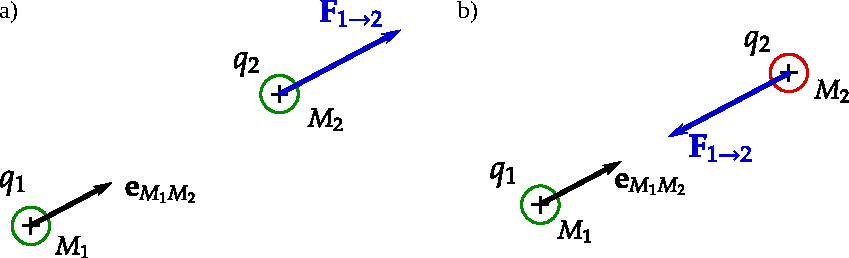
\includegraphics[scale=0.7]{coulomb.pdf}
	\caption{Force exercée par une charge $q_1$ sur une charge $q_2$ dans
	         le cas où les charges sont de même signe (à gauche) et de 
	 	signe opposé (à droite)}%
	\label{fig:coulomb}
\end{figure}


On remarque une forte ressemblance entre cette loi et la loi d'interaction gravitationnelle
proposée par Newton. Nous verrons que cette analogie, résumée par le Tableau~\ref{tab:analogie},
permet d'appliquer des résultats de l'électrostatique à la gravitation et inversement.
Néanmoins, l'interaction électrostatique fait apparaître deux types de charges
électriques et peut donc être soit attractive, soit répulsive. L'
interaction gravitationnelle est quant à elle toujours attractive.

\begin{table}[h!]
	\centering
	\caption{Tableau d'analogie entre force d'interaction électrique et 
	force d'interaction gravitationnelle. $\mathcal{G}$ est la constante 
	universelle de gravitation.}
	\label{tab:analogie}
	\begin{tabular}{c|c}
		Électrostatique 	&	Gravitation \\[1em] \hline \\[0.5em]
		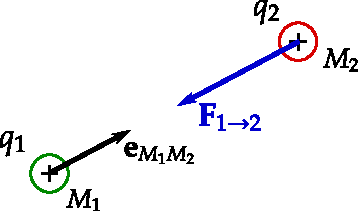
\includegraphics[scale=0.8]{analogie1.pdf} & 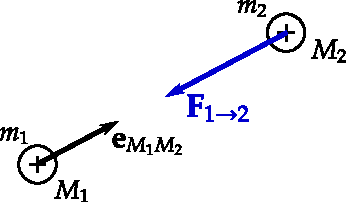
\includegraphics[scale=0.8]{analogie2.pdf} \\[2em]
		$\vecf_{1 \rightarrow 2} = \dfrac{1}{4\pi\epsilon_0}
	                                  \dfrac{q_1 q_2}{||M_1M_2||^2}
					  \mitbf{e}_{M_1M_2}$
					& $\vecf_{1 \rightarrow 2} = - \mathcal{G}
	                                  \dfrac{m_1 m_2}{||M_1M_2||^2}
					  \mitbf{e}_{M_1M_2}$ \\[1em]
		$q_1$			&	$m_1$ \\[1em]
		$\pieps$		&	$-\mathcal{G}$\\
	\end{tabular}
\end{table}

\begin{figure}[h!]
	\centering
	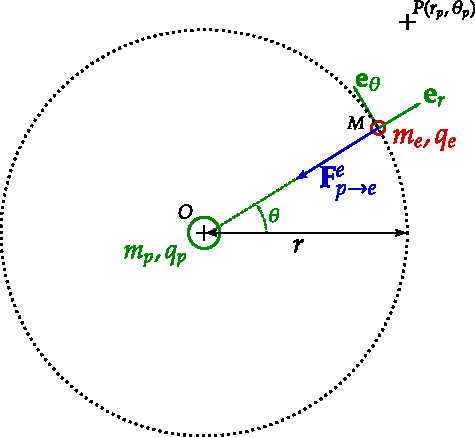
\includegraphics[scale=0.8]{modele_hydrogene}
	\caption{Modèle planétaire de l'atome d'hydrogène. L'électron 
	se trouve sur une orbite circulaire de rayon $r$ en pointillé ici.}%
	\label{fig:hydrogene}
\end{figure}

\begin{exemple}
	\label{ex:hydrogene}
	On considère le modèle planétaire de l'atome d'hydrogène 
	(voir Fig~\ref{fig:hydrogene}).
	Un électron de charge $-e = \unit{-1.60 \times 10^{-19}}{\coulomb}$ et 
	de masse $m_e \approx \unit{9.11 \times 10^{-31}}{\kilogram}$ décrit une
	orbite circulaire de rayon $r = \unit{52.9 \times 10^{-12}}{\meter}$
	autour d'un proton de charge $e$ et de masse
	$m_p \approx \unit{1.67 \times 10^{-27}}{\kilogram}$. 
	Les deux particules s'attirent car leurs charges sont de signe opposé. 
	On cherche à déterminer l'intensité 
	de la force électrostatique $\vecf^e_{p \rightarrow e}$ que le proton 
	exerce sur l'électron.
	La loi de Coulomb~\ref{eq:loi_coulomb} nous donne directement

	\begin{equation*}
		|\vecf^e_{p \rightarrow e}| = \dfrac{1}{4\pi\epsilon_0}
		                         \dfrac{e^2}{r^2}
					\approx \unit{82.7 \times 10^{-9}}{\newton}.
	\end{equation*}

	On peut alors comparer cette valeur à l'intensité de la force 
	d'interaction gravitationnelle
	$\vecf^g_{p \rightarrow e}$ que le proton exerce sur l'électron
	
	\begin{equation*}
		|\vecf^g_{p \rightarrow e}| = \mathcal{G}
		                         \dfrac{m_e m_p}{r^2}
					\approx \unit{36.2 \times 10^{-47}}{\newton},
	\end{equation*}
	avec $\mathcal{G} \approx \unit{6.67 \times 10^{-11}}{\newton \usk 
	\meter \squared \usk \rpsquare \kilogram}$ la constante universelle de
	gravitation. On remarque que l'intensité de la force 
	d'interaction gravitationnelle est bien plus faible que celle de la 
	force électrique, d'environ quarante ordres de grandeur.
	On néglige donc l'interaction gravitationnelle devant l'interaction
	gravitationnelle pour des
	particules chargées.
\end{exemple}


\section{Le champ électrostatique}
L'interaction gravitationnelle et l'interaction électrique ont posé problème aux 
physiciens du \textsc{xvii}\ieme~siècle car il s'agissait d'interaction à distance
sans contact. Faraday a donc introduit la notion de champ afin d'éviter 
ce délicat problème.
En physique, un champ est une fonction qui associe à tout point de l'espace un vecteur,
si le champ est vectoriel, ou un scalaire, si il est scalaire.
La température est par exemple un champ scalaire
et la vitesse est un champ vectoriel.
Une particule chargée exerce alors une force électrostatique sur une autre particule 
par l'intermédiaire du \emph{champ électrostatique} noté $\vece$.

\begin{defn}[Le champ électrostatique]
	Le champ électrostatique $\vece$ créé par une particule de charge $q$
	située au point $M$ de l'espace en un point $P$ est donné par

	\begin{equation}
		\vece(P) = \pieps \dfrac{q}{||MP||^2}\mitbf{e}_{MP},
	\end{equation}
	où $\mitbf{e}_{MP}$ est le vecteur unitaire dirigé de $M$ vers $P$.
	Le champ électrostatique est un champ vectoriel, à chaque point 
	de l'espace $P$, il associe un vecteur $\vece(P)$.
	Il s'exprime en $\volt \usk \reciprocal \meter$. 
	Connaissant la champ électrique en un point $P$ de l'espace, il est alors
	facile de déterminer la force $\vecf$ que subirait une particule de charge
	$Q$ placée en ce même point

	\begin{equation}
		\vecf = Q\vece(P).
	\end{equation}
\end{defn}

On peut déterminer le champ électrostatique 
créé en un point $P$ par un ensemble de $N$ particules chargées en utilisant
\emph{le principe de superposition}.
En effet, on constate expérimentalement que le champ électrostatique créé par ces
$N$ particules au point $P$ est égal à la somme de tous les champs
électrostatiques créés par toutes les charges.

\begin{defn}[Principe de superposition]
	On considère un ensemble de $N$ particules chargées. Chaque particule $i$
	porte la charge $q_i$ et se trouve en un point $M_i$ de l'espace. Chacune
	d'elle créé en un point $P$ de l'espace un champ électrostatique $\vece_i(P)$.
	Le champ électrostatique total créé au point $P$ est alors donné par 

	\begin{equation}
		\vece(P) = \sum_{i=1}^{N} \vece_i(P)
			 = \pieps \sum_{i=1}^{N} \dfrac{q_i}{||M_i P||^2}
			   \mitbf{e}_{M_i P}.
		\label{eq:superposition}
	\end{equation}
	De la même manière, la force $\vecf$ subit par une particule de charge $Q$ 
	située au point $P$ est alors donnée par
	\begin{equation}
		\vecf = Q \vece(P).
	\end{equation}
\end{defn}

\section{Les différentes distributions de charge}
Le plus souvent, la charge électrique est répartie de manière continue dans la 
matière. Dans ce cas, il est alors commode de définir une densité de charge qui
exprimera la quantité de charge contenue dans un volume, dans
une surface ou dans un fil. Chaque petit élément de volume, de surface ou de 
longueur renferme alors une charge notée $\mathrm{d}q$. Pour déterminer le 
champ électrique totale $\vece$ en un point $P$ de l'espace, 
il suffit alors de sommer les petits champs $\mathrm{\textbf{d}}\vece$ créés en $P$ 
par chaque petite charge $\mathrm{d}q$.

\begin{figure}
	\centering
	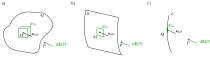
\includegraphics[scale=0.8]{distributions}
	\caption{Illustration de la notion de densité volumique (à gauche),
		 surfacique (milieu) et linéïque (à droite) de charge.}%
	\label{fig:distributions}
\end{figure}

\subsection{Densité volumique de charges}
	On considère une charge $Q$ répartie dans un volume $\mathcal{V}$
	(voir Fig.~\ref{fig:distributions}a). 
	On définit \textbf{
	la densité volumique de charge} $\rho$ 
	telle que pour tout point $M$ du volume,
	la charge $\mathrm{d}q$ contenue dans un petit volume $\mathrm{d}\tau_M$ centré 
	en $M$ est donnée par $\mathrm{d}q = \rho(M) \mathrm{d}\tau_M$.
	Elle s'exprime en $\coulomb \usk \rpcubic \meter$ et vérifie la relation
\begin{equation*}
	\iiint_{M \in \mathcal{V}} \rho(M) \mathrm{d}\tau_M = Q
\end{equation*}
En utilisant le principe de superposition, le champ électrostatique $\vece(P)$
créé au point $P$ de l'espace par une distribution volumique de charge $\rho$
contenue dans un volume $\mathcal{V}$ est
\begin{equation}
	\vece(P) = \pieps \iiint_{M \in \mathcal{V}} 
	\dfrac{\rho(M) \mathrm{d}\tau_M}{||MP||^2}\mitbf{e}_{MP},
\end{equation}
où $\dfrac{\rho(M) \mathrm{d}\tau_M}{||MP||^2}\mitbf{e}_{MP}$ est le champ 
électrique créé par le petit volume $\mathrm{d}\tau_M$ au point $P$.

\begin{exemple}
	On considère un noyau d'uranium $238$ de rayon $R = \unit{1}{\femto \meter}$.
	Il contient $92$ protons portant une charge $e$ et $146$ neutrons sans charge.
	On considère que la charge totale $Q$ du noyau est \textbf{uniformément répartie}
	dans le volume du noyau. La densité volumique de charge $\rho$ dans 
	le noyau d'uranium est donc donnée par

	\begin{equation*}
		\rho = \dfrac{Q}{\frac{4}{3}\pi R^3} = 
		\unit{35 \times 10^{27}}{\coulomb \usk \rpcubic \meter}
	\end{equation*}
\end{exemple}

\subsection{Densité surfacique de charge}
	On considère une charge $Q$ répartie sur une surface $\mathcal{S}$
	(voir Fig.~\ref{fig:distributions}b). 
	On définit \textbf{
	la densité surfacique de charge} $\sigma$ 
	telle que pour tout point $M$ de la surface,
	la charge $\mathrm{d}q$ contenue sur une petite surface $\mathrm{d}S_M$ centrée 
	en $M$ est donnée par $\mathrm{d}q = \sigma(M) \mathrm{d}S_M$.
	Elle s'exprime en $\coulomb \usk  \meter \rpsquared$ et vérifie la relation
\begin{equation*}
	\iint_{M \in \mathcal{S}} \sigma(M) \mathrm{d}S_M = Q
\end{equation*}
En utilisant le principe de superposition, le champ électrostatique $\vece(P)$
créé au point $P$ de l'espace par une distribution surfacique de charge $\sigma$
contenue sur une surface $\mathcal{S}$ est

\begin{equation}
	\vece(P) = \pieps \iint_{M \in \mathcal{S}} 
	\dfrac{\sigma(M) \mathrm{d}S_M}{||MP||^2}\mitbf{e}_{MP},
\end{equation}
où $\dfrac{\sigma(M) \mathrm{d}S_M}{||MP||^2}\mitbf{e}_{MP}$ est le champ 
électrique créé par la petite surface $\mathrm{d}S_M$ au point $P$.

\begin{exemple}
	Un condensateur de capacité $C = \unit{1}{\nano \farad}$ est alimenté 
	par une tension $U = \unit{10}{\volt}$. Cette tension induit une 
	accumulation de charges positives et négatives à la surface des deux 
	plaques des surface $S = \unit{2}{\milli \meter \squared}$
	qui le constituent. Une des plaques est alors chargée positivement
	avec la charge $Q = CU = \unit{10^{-8}}{\coulomb}$ 
	tandis que l'autre est chargée négativement avec la 
	charge $-Q$. Si on considère que la charge est \textbf{uniformément répartie}
	sur ces plaques, la densité surfacique de charge de la plaque positive
	est donnée par

	\begin{equation*}
		\sigma = \dfrac{Q}{S} = \unit{5 \times 10^{-3}}
		                        {\coulomb \usk \meter \rpsquared}
	\end{equation*}
\end{exemple}
\subsection{Densité linéïque de charge}
	On considère une charge $Q$ répartie sur un fil $\mathcal{L}$
	(voir Fig.~\ref{fig:distributions}c). 
	On définit \textbf{
	la densité linéïque de charge} $\lambda$ 
	telle que pour tout point $M$ du fil,
	la charge $\mathrm{d}q$ contenue sur une petite portion $\mathrm{d}\ell_M$ centrée 
	en $M$ est donnée par $\mathrm{d}q = \lambda(M) \mathrm{d}\ell_M$.
	Elle s'exprime en $\coulomb \usk \reciprocal \meter$ et vérifie la relation
\begin{equation*}
	\int_{M \in \mathcal{L}} \lambda(M) \mathrm{d}\ell_M = Q
\end{equation*}
En utilisant le principe de superposition, le champ électrostatique $\vece(P)$
créé au point $P$ de l'espace par une distribution surfacique de charge $\lambda$
contenue sur un fil $\mathcal{L}$ est

\begin{equation}
	\vece(P) = \pieps \int_{M \in \mathcal{L}} 
	\dfrac{\lambda(M) \mathrm{d}\ell_M}{||MP||^2}\mitbf{e}_{MP},
\end{equation}
où $\dfrac{\lambda(M) \mathrm{d}\ell_M}{||MP||^2}\mitbf{e}_{MP}$ est le champ 
électrique créé par la petite portion $\mathrm{d}\ell_M$ au point $P$.

\begin{exemple}
	Cette distribution est plus difficile à imaginer.
	On peut par exemple la réaliser en fixant des 
	ions métalliques sur une chaîne de polymères. On considère une chaîne de
	polymère présentant une longueur $L$ de $\unit{1}{\micro \meter}$. On a 
	fixé des ions $Fe^+$ à trois atomes d'intervalle sur cette chaîne.
	La charge est donc répartie de manière uniforme le long du polymère.
	La taille d'un atome étant d'environ $\unit{10^{-10}}{\meter}$, la chaîne de 
	polymère est composée d'environ $10^4$ atomes. Elle porte
	donc une charge totale $Q$ qui vaut $10^4 \times 1.6 \times 10^{-19}/3$.
	On peut alors déduire la
	densité linéïque de charge $\lambda$ de cette chaîne
	\begin{equation}
		\lambda = \dfrac{Q}{L} \approx \dfrac{10^{-6}\times 10^{10}
			           \times 1.6 \times 10^{-19}/3}{10^{-6}}
				= \unit{5.3 \times 10^{-10}}{\coulomb \usk
				   \reciprocal \meter}
	\end{equation}
	où $Q$ est la charge totale fixée sur le polymère.
\end{exemple}

\begin{attention}
	Une distribution volumique de charge est en $\coulomb \usk \rpcubic \meter$,
	une distribution surfacique en $\coulomb \usk \meter \rpsquared$
	et une distribution linéïque en $\coulomb \usk \reciprocal \meter$.
\end{attention}

\section{Équation de l'électrostatique}
On considère une charge ponctuelle $Q$ située à l'origine d'un repère sphérique
$(O, \er, \etheta, \ephi)$ (voir Fig.~\ref{fig:gauss}a). Le champ électrique créé 
par cette charge en 
un point $M(r, \theta, \phi)$ est donné par

\begin{equation*}
	\vece(M) = \pieps \dfrac{Q}{||OM||^2}\er 
	         = \dfrac{Q}{4\pi\epsilon_0 r^2}\er.
\end{equation*}
Nous allons nous servir de cet exemple simple pour retrouver certaines propriétés
spatiales du champ électrostatique.

\begin{figure}
	\centering
	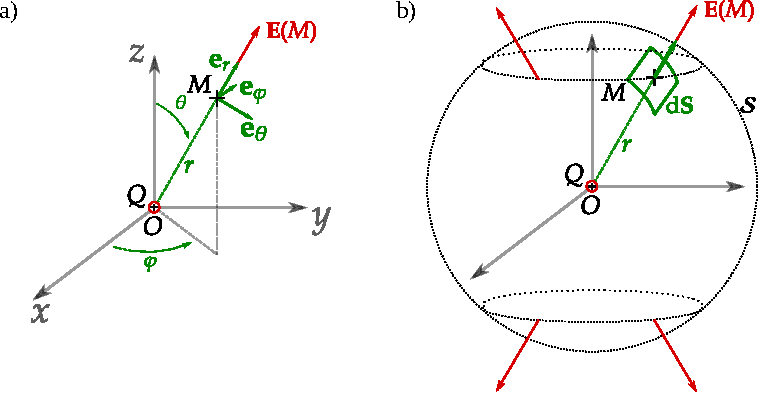
\includegraphics[width=0.8\linewidth]{gauss}
	\caption{Champ créé par une charge ponctuelle $Q > 0$ située en 
		 $O$ au point $M$ (à gauche) et sphère $\mathcal{S}$ à travers
	 	 laquelle on calcule le flux du champ de la charge $Q$ (à droite).
	         $\mathrm{d}\mathbf{S}$ représente un élément infinitésimal 
	 	 de la surface.}%
	\label{fig:gauss}
\end{figure}

\subsection{Le théorème de Gauss}
\label{sec:gauss}
Le théorème de Gauss est un outil puissant qui va nous permettre de calculer
facilement le champ électrique généré par une distribution de charges simple.
Pour le mettre en place, nous
cherchons dans un premier temps à déterminer ``la quantité'' de champ électrique 
$E$ qui traverse une
sphère $\mathcal{S}$ de rayon $r$ centrée en $O$ à laquelle $M$ 
appartient (voir Fig.~\ref{fig:gauss}b). 
La surface $\mathcal{S}$ est ici une surface \textbf{fermée}.

\begin{defn}[Surface fermée]
	Une surface est dite fermée si elle délimite un volume intérieur 
	et un volume extérieur. La surface d'une feuille de papier n'est par 
	exemple pas une surface fermée alors que la surface d'un ballon de baudruche
	en est une.
\end{defn}

On commence alors par déterminer 
l'expression du vecteur surface élémentaire $\mathrm{d}\mathbf{S}$. 

\begin{defn}[Vecteur surface élémentaire]
	À chaque élément d'aire $\mathrm{d}S$ centré en $M$ de la surface $\mathcal{S}$, 
	on  affecte un vecteur surface élémentaire $\mathrm{d}\mathbf{S}$ 
	qui vérifie les propriétés suivantes
	\begin{itemize}
		\item il a pour norme l'aire du petit élément de surface centré 
		  au point $M$. Il est donc homogène à une surface.
		\item il est orthogonal à la surface.
		\item il doit être orienté. Cette orientation est au choix de 
		  l'utilisateur.
	\end{itemize}
\end{defn}

\begin{attention}
	Une surface en physique doit toujours être orientée pour savoir
	si le flux qu'on calcule est un flux entrant ou sortant.
\end{attention}

$\mathcal{S}$ est une sphère de rayon $r$ fixé, pour se déplacer à la surface 
de cette dernière, 
il suffit dont de faire varier $\theta$ et $\phi$. $\mathrm{d}\mathbf{S}$ 
étant orthogonal à la surface $\mathcal{S}$, on a

\begin{equation*}
	\ds = r^2 \sin \theta \dtheta \dphi \er.
\end{equation*}
Pour déterminer la quantité de champ électrique qui sort de la surface 
$\mathcal{S}$, on introduit la notion de flux. On retrouve cette notion en géographie,
 où le flux migratoire exprime le nombre de personnes entrant ou sortant d'un 
 pays.

\begin{defn}[Flux d'un champ de vecteurs]
	Soit $M$ un point d'un surface fermée en lequel règne un champ $\vece(M)$.
	Soit $\mathrm{d}\mathbf{S}$ le vecteur surface élémentaire sortant associé
	à l'élément de surface centré en $M$. \textbf{Le flux sortant élémentaire} du 
	vecteur $\vece$ à travers $\mathrm{d}S$ est donné par
	$\vece(M) \cdot \mathrm{d}\mathbf{S}$.

	\textbf{Le flux total sortant} d'un champ de vecteur $\vece$ à travers 
	une surface fermée
	$\mathcal{S}$ est simplement la somme sur tous les éléments de la surface de tous
	les flux élémentaires sortants
	\begin{equation}
		\oiint_{M \in \mathcal{S}} \vece(M) \cdot \mathrm{d}\mathbf{S}.
	\end{equation}
	Il s'exprime en $\volt \usk \meter$. Le flux est une grandeur algébrique
	qui peut-être positive ou négative. Le symbole $\oiint$ signifie que
	l'intégrale est réalisée sur une surface fermée, il n'est pas obligatoire.
\end{defn}

Le flux de $\vece$ à travers $\mathcal{S}$ s'écrit alors

\begin{equation}
	\oiint_\mathcal{S} \vece \cdot \ds = \oiint_\mathcal{S} \dfrac{Q}{4\pi\epsilon_0 r^2}
	                       r^2 \sin \theta \dtheta \dphi \er \cdot \er
			     = \dfrac{Q}{4 \pi \epsilon_0} \int_0^\pi \sin \theta \dtheta
			     \int_0^{2\pi} \dphi
			     = \dfrac{Q}{\epsilon_0}.
\end{equation}
Ce flux est sortant si la charge $Q$ est positive et est entrant si la charge
$Q$ est négative.
On constate alors que le flux du champ électrique à travers la sphère $\mathcal{S}$
de rayon $r$ ne dépend que de la charge $Q$ qu'elle contient et pas de son rayon.
Cette propriété que nous venons de montrer pour une charge ponctuelle est en 
fait une propriété du champ électrique connue sous le nom de \textbf{théorème de 
Gauss}.

\begin{defn}[Théorème de Gauss]
	Le flux du champ électrique $\vece$ à travers une surface fermée $\mathcal{S}$, 
	qui délimite un volume $\mathcal{V}$, est égale à la charge incluse $Q$ dans
	ce volume, divisé par $\epsilon_0$

	\begin{equation}
		\oiint_\mathcal{S} \vece \cdot \ds = \dfrac{Q}{\epsilon_0}.
		\label{eq:gauss}
	\end{equation}
	La surface $S$ est appelée la \textbf{surface de Gauss}.
\end{defn}

Le théorème de Gauss peut-être traduit sous une forme locale, 
appelée l'\textbf{équation de 
Maxwell-Gauss}, qui relie alors le champ électrique à la distribution de charge.

\begin{defn}[Équation de Maxwell-Gauss]
	L'équation de Maxwell-Gauss relie le champ électrique $\vece$ à la 
	distribution de charge $\rho$

	\begin{equation}
		\div \vece = \dfrac{\rho}{\epsilon_0}.
		\label{eq:MG}
	\end{equation}
	La divergence de $\vece$ est une grandeur \textbf{scalaire}. 
	Cette équation est une relation \textbf{locale}, elle permet de relier
	les dérivées spatiale du champ électrique en un point de l'espace à 
	la densité volumique de charge en ce même point.
\end{defn}

\subsection{Le potentiel électrostatique et l'équation de Maxwell-Faraday}
On cherche maintenant à calculer le rotationnel du champ. 
Cela donne en 
coordonnées sphériques

\begin{equation*}
	\rot \vece = \dfrac{1}{r \sin \theta}\left[\dfrac{1}{r}
		\dfrac{\partial}{\ddtheta}(\sin \theta E_\varphi) - 
	        \dfrac{\partial E_\theta}{\ddphi}\right]\er + 
		\left[\dfrac{1}{r\sin \theta}\dfrac{\partial E_r}{\ddphi} -
		\dfrac{1}{r}\dfrac{\partial}{\ddr}\left(rE_\varphi\right)\right]\etheta
		+ \dfrac{1}{r}\left[\dfrac{\partial}{\ddr}(r E_\theta)
		- \dfrac{\partial E_r}{\ddtheta}\right]\ephi,
\end{equation*}
où $E_r$, $E_\theta$ et $E_\varphi$ sont respectivement les composantes de
$\vece$. Ici, $E_r$ ne dépend que de $r$ et les composantes $E_\theta$ et 
$E_\varphi$ sont nulles. On a donc 

\begin{equation*}
	\rot \vece = \mitbf{0}.
\end{equation*}
Ce résultat se généralise à un champ électrostatique $\vece$ quelconque sous la
forme de l'équation de Maxwell-Faraday.

\begin{defn}[Équation de Maxwell-Faraday]
	Un champ électrique $\vece$ en \textbf{régime statique}, c'est-à-dire
	indépendant du temps, vérifie 
	\begin{equation}
		\rot \vece = \mitbf{0}.
	\end{equation}
	Le rotationnel de $\vece$ est une grandeur \textbf{vectorielle}. Comme
	l'équation de Maxwell-Gauss, l'équation de Maxwell-Faraday est 
	une relation \textbf{locale} vérifiée
	en tout point de l'espace.
\end{defn}

Comme l'équation de Maxwell-Gauss, l'équation de Maxwell-Faraday peut se mettre 
sous une forme intégrale, en exprimant la circulation du champ électrique sur
une courbe fermée $\mathcal{C}$.

\begin{defn}[Circulation d'un champ de vecteurs]
	Soit $\mathbf{W}$ un champ de vecteur et $\mathcal{C}$ un arc de courbe orienté 
	dans l'espace. On appelle circulation du champ de vecteurs $\mathbf{W}$
	le long de $\mathcal{C}$ la quantité
	\begin{equation*}
		\int_{M \in \mathcal{C}} \mathbf{W}(M) \cdot \dl_M.
	\end{equation*}
\end{defn}

\begin{attention}
	Un contour doit toujours être orienté !
\end{attention}

\begin{defn}[Circulation du champ électrostatique]
La circulation du champ électrostatique $\vece$ le long d'un contour fermé
orienté $\mathcal{C}$ est nul
\begin{equation}
	\oint_\mathcal{C} \vece \cdot \dl = 0.
\end{equation}
On dit alors que le champ électrique est à circulation \textbf{conservative}.
\end{defn}

Le champ électrostatique est donc un champ dont le rotationnel est nul en tout 
point de l'espace. L'analyse vectorielle affirme qu'il est possible dans ce cas 
de définir un champ scalaire $V$,
défini à une constante près, 
tel que $\vece = -\gradient V$.

\begin{defn}[Potentiel électrostatique]
	Le champ électrostatique étant à rotationnel nul, il existe un 
	champ scalaire $V$, appelé \textbf{potentiel électrostatique}, tel qu'en
	tout point de l'espace

	\begin{equation}
		\vece = -\gradient V.
		\label{eq:potentiel}
	\end{equation}
	Le potentiel électrostatique s'exprime en volts. Il est toujours défini
	à une constante près.
	La circulation du 
	champ électrostatique entre un point $A$ et un point $B$ est alors donnée
	par

	\begin{equation}
		\int_A^B \vece \cdot \dl = V(A) - V(B)
	\end{equation}
\end{defn}

En reportant $\vece$ par $-\grad V$ dans l'équation de 
Maxwell-Gauss~\ref{eq:MG}, on obtient

\begin{equation*}
	\div(-\grad V) = \dfrac{\rho}{\epsilon_0} \Rightarrow \laplacien V = 
	              -\dfrac{\rho}{\epsilon_0}.
\end{equation*}

\begin{defn}[Équation de Poisson]
	Le potentiel électrique suit l'\textbf{équation de Poisson}
	\begin{equation}
		\laplacien V = -\dfrac{\rho}{\epsilon_0}.
	\end{equation}
\end{defn}

De plus, la force électrostatique est une \textbf{force conservative}. On peut alors
définir une \textbf{énergie potentielle} qui lui est associée.

\begin{defn}[Énergie potentielle électrostatique]
	La force électrostatique $\vecf$ est une force conservative, elle 
	dérive donc d'une énergie potentielle $E_p$

	\begin{equation}
		\vecf = - \gradient E_p.
	\end{equation}
	Cette énergie est définie à une constante
	près. Elle s'exprime en joule ($\kilogram \usk \meter \squared \usk \second
	\squared$ en SI). Une charge $q$ placée en un point $M$ de
	l'espace où règne un potentiel électrostatique $V$ possède une 
	énergie potentielle électrostatique 

	\begin{equation*}
		E_p = q V(M) + X,
	\end{equation*}
	où $X$ est une constante. Elle est soumise à la force électrostatique

	\begin{equation*}
		\vecf = -\gradient E_p.
	\end{equation*}
\end{defn}

\begin{exemple}
	Dans l'Exemple~\ref{ex:hydrogene} du modèle planétaire
	de l'atome d'hydrogène, le proton génère
	un potentiel $V$
	\begin{equation*}
		V(r) = \dfrac{e}{4 \pi \epsilon_0 r}.
	\end{equation*}
	L'électron possède donc une énergie potentielle $E_p$ donnée par
	\begin{equation*}
		E_p(r) = -eV(r) = \dfrac{-e^2}{4 \pi \epsilon_0 r} + C,
	\end{equation*}
	où $C$ est une constante. Nous posons $C = 0$, ce qui nous permet d'obtenir une énergie
	potentielle qui est nulle lorsque $r$ tend vers l'infini. L'électron 
	possède alors une énergie potentielle
	$E_p \approx \unit{-27.3}{\electronvolt}$,
        où $\unit{1}{\electronvolt} \approx \unit{1.60 \times 10^{-19}}{\joule}$.
	L'application du principe fondamental de la dynamique à l'électron permet
	de déterminer la vitesse de ce dernier dans le référentiel d'étude.
	On peut alors en déduire son énergie cinétique
	\begin{equation*}
		E_c = \dfrac{e^2}{8 \pi \epsilon_0 r} = \unit{13.7}{\electronvolt}.
	\end{equation*}
	Finalement, l'électron possède une énergie totale de $-\unit{13.6}{\electronvolt}$.
\end{exemple}

\section{Étude des lignes de champ de \vece}
Nous nous intéressons dans cette partie aux propriétés spatiales du champ $\vece$.
Nous allons voir comment les \textbf{lignes de champ} nous renseignent sur sa répartition 
dans l'espace.

\begin{defn}[Ligne de champ]
	Une ligne de champ est une courbe tangente en chaque point au vecteur 
	du champ de vecteurs considéré, orientée dans le sens du champ. Deux
	lignes de champ ne peuvent pas se croiser.
\end{defn}

Pour déterminer l'équation de ces lignes de champ, il suffit de résoudre l'équation
qui traduit la tangence en tout point de l'espace $M$ des lignes de champ 
au vecteur $\vece(M$)

\begin{equation}
	\vece \times \dl = \mitbf{0},
\end{equation}
où $\dl$ est un élément de la ligne de champ.



\begin{exemple}
	Les lignes du champ électrostatique $\vece$ généré par une charge ponctuelle $q$
	sont des droites portées par un rayon de la charge (voir Fig~\ref{fig:lignes}). 
	Si la charge est positive, elles sont orientées vers l'extérieur. À
	l'inverse si elle
	est négative, elles sont orientés vers la charge. On cherche à déterminer l'équation
	de ces lignes de champ. On se place dans un repère sphérique $(\er, \etheta, \ephi)$
	centré sur le centre de la charge $q$. Un point de l'espace $M$ est donc repéré par
	ses coordonnées $(r, \theta, \varphi)$. Un élément $\dl$ de la ligne de champ 
	passant par $M$ doit vérifier
	\begin{equation*}
		\vece(M) \times \dl = \mitbf{0} \Rightarrow
		\dfrac{q}{4 \pi \epsilon_0}
		\begin{array}{|l}
			1/r^2 \\[1em]
			0 \\[1em]
		0 \\
		\end{array}
		\times
		\begin{array}{|l}
			\dr \\[1em] 
			r \dtheta \\[1em]
			r \sin \theta \dphi \\
		\end{array}
		= \mitbf{0}
		\Rightarrow
		\begin{array}{|l}
			0 \\[1em] 
			\sin \theta \dphi/r \\[1em]
			\dtheta/r \\
		\end{array}
		= \mitbf{0}
		\Rightarrow
		\left\{
		\begin{array}{rcl}
			\sin \theta \dphi/r = 0 \\[1em]
			\dtheta/r = 0 \\
		\end{array}
		\right.
	\end{equation*}
En d'autres termes, tous les points de cette ligne de champ doivent avoir le 
même $\theta$ et le même $\varphi$. Les lignes de champ sont donc bien portées 
par des rayons de la charge.
\end{exemple}

\begin{figure}[h!]
	\centering
	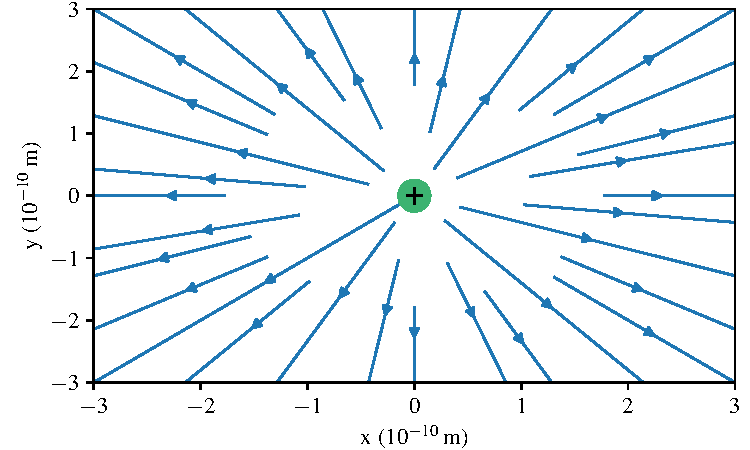
\includegraphics[width=0.45\linewidth]{charge+}
	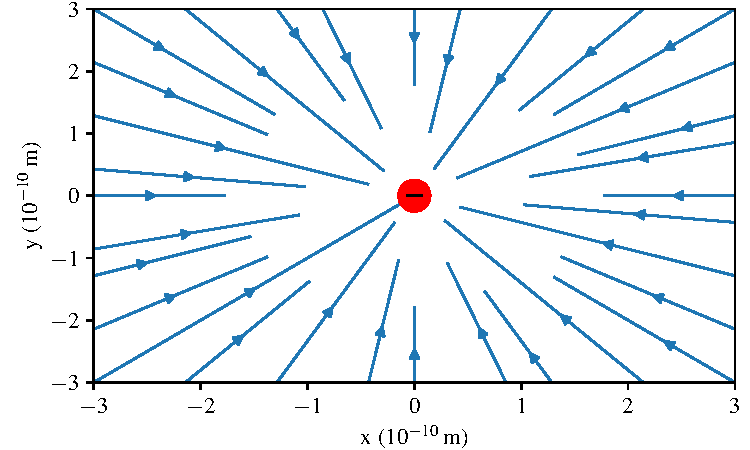
\includegraphics[width=0.45\linewidth]{charge-}
	\caption{Ligne du champ $\vece$ créé par une charge positive (à gauche)
	         et par une charge négative (à droite).}%
	\label{fig:lignes}
\end{figure}

Nous allons maintenant considérer la cas d'un proton et d'un électron séparé 
par une distance de $\unit{0.2}{\nano \meter}$ (voir Fig.~\ref{fig:dipole}).
Les lignes de champ nous permettent de retrouver quelques propriétés du champ 
électrostatique énoncées précédemment.

\begin{figure}[h!]
	\centering
	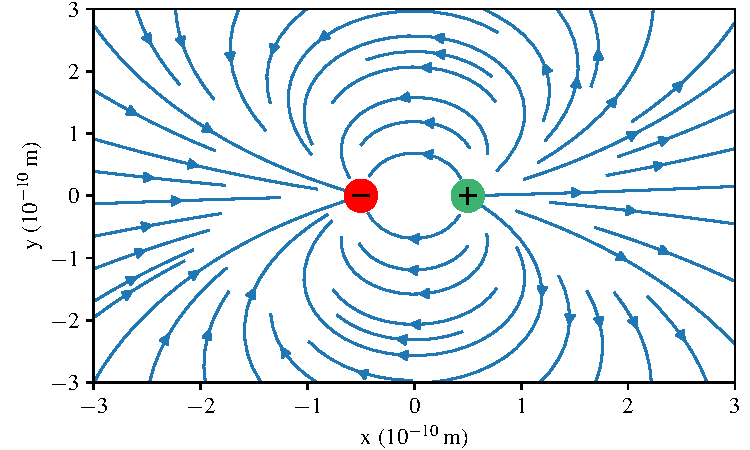
\includegraphics[scale=0.75]{dipole}
	\caption{Lignes du champ électrique généré par un proton (charge verte) et 
	         un électron (charge rouge).}%
	\label{fig:dipole}
\end{figure}

\begin{enumerate}
	\item On remarque tout d'abord que les lignes de champ sont orientées 
	  de la \textbf{charge positive vers la charge négative}. Cette première 
	  observation peut être vue comme une conséquence de la relation reliant 
	  le champ électrique $\vece$ et le potentiel électrostatique $V$ 
	  (voir Eq.~\ref{eq:potentiel}). En effet, le sens de $\vece$ est 
	  opposé à celui du gradient de $V$ (comme le traduit le signe $-$ dans 
	  l'expression).
	  La ligne de champ s'écoule donc du potentiel le plus élevé 
	  vers le moins élevé.
      \item La divergence d'un champ vectoriel permet de mesurer
	    le flux de ce dernier à travers un volume. Si elle est nulle, 
	    une ligne de champ entrant dans un volume doit absolument en ressortir.
	    La divergence non nulle du champ électrique (voir Eq.~\ref{eq:MG})
	    se traduit par la possibilité pour les lignes de champ d'émerger d'un 
	    volume (du proton ici) et de converger dans un volume (l'électron ici).

	    \item Le rotationnel d'un champ vectoriel traduit la tendance de ce dernier
	    à tourner autour d'un point.
	    Le rotationnel nul du champ électrique se traduit par l'impossibilité
	    pour les lignes de champ de tourner autour d'un point. Une ligne du champ
	    électrique ne peut donc pas reboucler sur elle-même.

    	   \item Grâce aux lignes de champ, on retrouve rapidement les plans de 
		 symétrie et d'antisymétrie du champ électrique. Le plan médiateur 
		 est par exemple un plan d'antisymétrie du champ électrique. 
		 L'analyse de ces symétries sera utile pour calculer le champ
		 électrique d'une distribution de charge.
\end{enumerate}

\section{Calcul du champ électrostatique}
\label{sec:calcul_e}
Nous allons voir dans cette partie comment nous pouvons utiliser le théorème de
Gauss pour calculer le champ électrique créé 
par une distribution de charges simple. Nous nous intéressons ici à une boule de
rayon $R_1$ et de centre $O_1$ uniformément chargée avec une densité volumique
de charge $\rho > 0$ (voir Fig.~\ref{fig:cavite1}). On cherche à déterminer 
l'expression du champ électrique $\vece$ en un point $M$ de l'espace. Pour ce faire, 
il suffit de suivre le mode d'emploi suivant
\begin{enumerate}
	\item Faire un schéma du système ! C'est absolument indispensable
	  (voir Fig.~\ref{fig:cavite1})
	\item Choisir un repère adapté au problème
	\item Étudier les invariances de cette distribution
	\item Étudier les symétries de la distribution de charges à l'origine 
	  du champ électrique
	\item Choisir une surface de Gauss et appliquer le théorème de Gauss.
\end{enumerate}

Nous choisissons ici d'utiliser un repère sphérique $(O_1, \er, \etheta, \ephi)$.
Le point $M$ est donc repéré par ses coordonnées $(r, \theta, \phi)$. Le champ
électrique en $M$ s'écrit de manière générale

\begin{equation}
	\vece(M) = E_r(M)\er + E_\theta(M)\etheta + E_\varphi(M)\ephi.
	\label{eq:cavite1}
\end{equation}
Le champ électrique est un vecteur à trois composantes et chaque composante
dépend des coordonnées de $M$. Pour simplifier cette expression, il est intéressant
de considérer les invariances et symétries de la distribution de charge qui génère
le champ $\vece$.

\begin{figure}
	\centering
	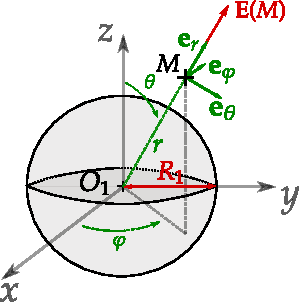
\includegraphics[scale=1]{cavite1}
	\caption{Schéma de la cavité uniformément chargée.}%
	\label{fig:cavite1}
\end{figure}

\subsection{Invariance de la distribution de charges}
On cherche ici à savoir si la distribution de charge est modifiée sous l'effet
d'une translation ou d'une rotation de l'espace. En d'autres termes, on regarde
de quelles variables dépend la densité de charge $\rho$. Étant donné que la
sphère est ici uniformément chargée, on observe que

\begin{itemize}
	\item  si je tourne la sphère d'un angle $\Delta \theta$ dans la
	  direction $\etheta$, le problème
	  ne change pas. La distribution de charge est donc invariante 
	  par rotation selon l'angle $\theta$. $\vece$ \textbf{ne dépend pas de
	  $\mitbf{\theta}$}.

	  \item  si je tourne la sphère d'un angle $\Delta \varphi$ dans la
	  direction $\ephi$, le problème
	  ne change pas. La distribution de charge est donc invariante 
	  par rotation selon l'angle $\varphi$. $\vece$ \textbf{ne dépend pas de
	  $\mitbf{\varphi}$}.
  	\item si je déplace la sphère d'une distance $\Delta r$ dans la direction
	$\er$ je remarque que le problème change. Par exemple si $\Delta r$ 
	est supérieur à $R_1$, le point $O_1$ n'appartient plus à la sphère après
	la translation. $\vece$ \textbf{dépend de} $\mitbf{r}$.

\end{itemize}

Finalement, l'expression~\ref{eq:cavite1} du champ électrique se simplifie

\begin{equation}
	\vece(M) = E_r(r)\er + E_\theta(r)\etheta + E_\varphi(r)\ephi.
\end{equation}
\subsection{Symétries de la distribution de charges}

\begin{defn}[Principe de Curie]
	Lorsque les causes produisent des effets, les symétries présentes dans les
	causes doivent se retrouver dans celles des effets.
\end{defn}

Si on applique ce principe au champ électrique créé par une distribution 
de charges, cela revient à dire que les symétries de la distribution de 
charges doivent se retrouver dans les symétries du champ électrique. On en 
déduit les règles suivantes

\begin{defn}[Symétries de $\vece$ et de la distribution de charge]
  \begin{itemize}
  \item si $(\Pi)$ est un plan de symétrie de la distribution de charge et que 
    $M$ appartient à $(\Pi)$, alors obligatoirement $\vece(M)$ doit 
    appartenir à $(\Pi)$,
  \item si $(\Pi)$ est un plan d'antisymétrie de la distribution de charge 
    et que $M$ appartient à $(\Pi)$, alors obligatoirement $\vece(M)$ doit 
    être orthogonal à $(\Pi)$.
  \end{itemize}
\end{defn}

Pour appliquer ces règles à notre exemple, on détermine les plans de symétrie 
et d'antisymétrie de la distribution de charges auxquels 
le point $M$ appartient

\begin{itemize}
	\item le plan $(M, \er, \etheta)$ est un plan de symétrie de la distribution
		de charge. $\vece(M)$ \textbf{doit donc appartenir à ce plan}.
        \item le plan $(M, \er, \ephi)$ est un plan de symétrie de la distribution de 
		charge. $\vece(M)$ \textbf{doit donc appartenir à ce plan}.
\end{itemize}

$\vece(M)$ doit appartenir au plan $(M, \er, \etheta)$ et au plan $(M, \er, \ephi)$.
$\vece$ doit donc être colinéaire à $\er$

\begin{equation}
	\vece(M) = E_r(r) \er.
\end{equation}
Nous n'avons imposé aucune condition sur la position de $M$, cette relation est
donc vraie pour tout point $M$ de l'espace. Maintenant que l'expression du 
champ électrique a été simplifiée au maximum, on cherche à appliquer le théorème
de Gauss.

\subsection{Application du théorème de Gauss}
\begin{figure}
	\centering
	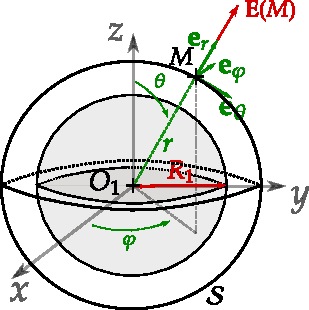
\includegraphics[scale=1]{cavite1_gauss}
	\caption{Schéma de la cavité avec la surface de Gauss $\mathcal{S}$
	         qui est une sphère de rayon $r$ et de centre $O_1$. $M$
	         appartient à cette surface.}%
	\label{fig:cavite_gauss}
\end{figure}

La distribution de charge présente une symétrie sphérique. On choisit comme surface 
de Gauss une sphère de rayon $r$ et de centre $O_1$ 
(voir Fig~\ref{fig:cavite_gauss}) et on applique le théorème de Gauss sur cette
sphère

\begin{equation}
	\oiint_\mathcal{S} \vece(M) \cdot \ds = \dfrac{Q}{\epsilon_0},
	\label{eq:cavite_gauss}
\end{equation}
où $Q$ est la charge contenue à l'intérieur de $\mathcal{S}$. On commence
par déterminer l'expression du membre de gauche. Comme nous l'avons vu 
(voir Sec.~\ref{sec:gauss}), dans le cas d'une sphère,

\begin{equation}
	\ds = r^2 \sin \theta \dtheta \dphi \er.
\end{equation}
On obtient alors
\begin{equation}
	\oiint_\mathcal{S} \vece(M) \cdot \ds = 
	\oiint_\mathcal{S} E(r) \er \cdot r^2 \sin \theta \dtheta \dphi \er
	= E(r) r^2 \int_0^{2 \pi} \dphi \int_0^\pi\sin \theta \dtheta
	= 4 \pi E(r) r^2.
\end{equation}
On s'intéresse maintenant au terme de droite de l'équation~\ref{eq:cavite_gauss}.
La charge $Q$ est uniformément répartie dans la sphère de rayon $R_1$, on a donc

\begin{equation}
	\rho(r) = 
	\left\{
	\begin{array}{l}
		0,\ \mathrm{si} \  r > R_1,\\[1em]
		\dfrac{Q}{\dfrac{4}{3} \pi r^3},\ \mathrm{si} \ r \leq R_1. \\
	\end{array}
	\right.
\end{equation}
On a alors deux cas de figure
\begin{enumerate}
	\item si $r \leq R_1$, $Q = \dfrac{4}{3 \epsilon_0} \pi r^3 \rho$
	  $\Rightarrow \vece(r) = \dfrac{\rho r}{3 \epsilon_0} \er$.
	\item si $r > R_1$, $Q = \dfrac{4}{3} \pi R_1^3 \rho$ 
	  $\Rightarrow \vece(r) = \dfrac{\rho R_1^3}{3 \epsilon_0 r^2} \er$.
\end{enumerate}

\begin{rem}
	Si on remplace $\rho$ par son expression en fonction de $Q$, 
	$\rho = \dfrac{3Q}{4 \pi R_1^3}$, dans la deuxième 
	situation, on retrouve le champ électrique généré par une charge ponctuelle.
\end{rem}

\nocite{*}
\putbib[Chapitre_1/electrostatique]
\newpage
\section{Exercices}
\begin{exocor}[Potentiel de Yukawa]
	Le physicien japonais Yukawa a postulé la forme d'un potentiel pour modéliser
	les interactions entre particules dans un noyau atomique. Nous étudions
	ici ce potentiel comme s'il s'agissait d'un potentiel électrostatique.

	Dans un repère sphérique $(\er, \etheta, \ephi)$, une distribution de 
	charge à symétrie sphérique crée, à une distance $r$,
	un potentiel électrostatique de la forme
	\begin{equation}
		V(r) = \dfrac{Q}{4 \pi \epsilon_0 r} \exp\left(-\dfrac{r}{a}\right),
	\end{equation}
	$Q$ et $a$ étant des constantes positives.

	\begin{enumerate}
		\item Déterminer les unités de $Q$ et de $a$.
		\item Déterminer le champ électrostatique correspondant.
		\item En déduire la charge $q(r)$ contenue dans une sphère de 
		  rayon $r$ et de centre $O$.
		\item Déterminer $q(r)$ dans les deux cas extrêmes
			\begin{enumerate}
				\item $r$ tend vers zéro,
				\item $r$ tend vers $\infty$
			\end{enumerate}
		 En déduire qualitativement la nature de la distribution de charge
		 et donner une interprétation de $a$.
 	\end{enumerate}
\end{exocor}

\begin{exocor}[Champ gravitationnel dans une cavité]
Un modèle de Terre de rayon $R_1$ et de centre $O_1$ possède une masse volumique 
$\rho>0$ uniforme sauf dans une cavité sphérique, 
entièrement incluse dans la boule, centrée en $O_2$, de rayon $R_2$
(voir Fig~\ref{fig:cavite}). 

On cherche le champ gravitationnel $\vecg(M)$ en un point $M$ 
à l'intérieur de la cavité.
Dans un premier temps, on ignore la présence de la cavité.
\begin{enumerate}
	\item Rappeler l'expression du champ électrostatique $\vece$ générée par une
	  charge $q$ et du champ gravitationnel $\vecg$ générée par une particule
	  de masse $m$ en un point $P$ de l'espace. 
	  En déduire un tableau d'analogie entre interaction
	  gravitationnelle et interaction coulombienne.
  	\item En déduire un théorème de Gauss pour le champ gravitationnel
	  $\vecg$.
	\item Étudier les symétries et invariances du système en l'absence de
	  la cavité creuse.
	\item En appliquant le théorème de Gauss, déterminer l'expression
	  du champ $\vecg$ en un point $M$ de l'espace.
	  Vérifier l'homogénéité de l'expression obtenue.
	\item Étudier les symétries et invariances du système avec la cavité.
	  Pensez-vous qu'il soit judicieux d'utiliser le théorème de Gauss
	  ici ?
	\item En vous servant du théorème de superposition, 
	  déterminer le champ $\vecg$ en un point $M$ à l'intérieur de la cavité.
\end{enumerate}
\end{exocor}
\begin{figure}[h!]
\centering
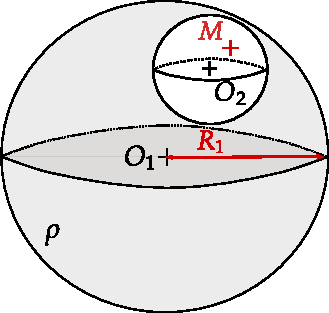
\includegraphics[scale = 0.6]{cavite.pdf}
\caption{Schéma de la sphère de masse volumique $\rho$ (en gris sur le schéma) 
	 et de la cavité vide (en blanc).
         À l'intérieur de la cavité, la masse volumique vaut 0.}
\label{fig:cavite}
\end{figure}

\begin{exocor}[Fil chargé]
	Calculer le champ électrostatique créé par un fil rectiligne infini
	uniformément chargé avec une densité linéïque de charge $\lambda$, en 
	tout point de l'espace.
\end{exocor}


\begin{corr}{Électrostatique}
\correction{Potentiel de Yukawa}
\begin{enumerate}
	\item L'argument d'une fonction est toujours sans dimension. \fbox{$a$ est donc
	  homogène à une longueur.} Le terme 
	  \begin{equation*}
	  	\dfrac{Q}{4 \pi \epsilon_0 r}
	 \end{equation*}
	  correspond au potentiel électrostatique généré par une charge ponctuelle.
	  On en déduit que \fbox{$Q$ est homogène à une charge.}

  	\item Le champ électrostatique $\vece$ est lié au potentiel $V$ par la
          relation suivante
	  \begin{equation*}
		  \vece = - \grad(V),
	  \end{equation*}
	  qui est vraie en tout point de l'espace. On a alors
	  \begin{equation*}
		  \vece(r) = - \dd{V}{r}(r)\er -\dfrac{1}{r}\dd{V}{\theta}(r)\etheta
		  -\dfrac{1}{r\sin\theta}\dd{V}{\phi}(r)\ephi
		  = \boxed{\dfrac{Q}{4 \pi \epsilon_0 r^2}\exp\left(-\dfrac{r}{a}
		    \right)\left(1 + \dfrac{r}{a}\right)\er}
	  \end{equation*}

  	\item On considère une sphère $\mathcal{S}$ de rayon $r$ et de centre $O$.
	  Cette sphère forme une surface fermée, on peut donc lui appliquer le
	  théorème de Gauss pour connaître la charge $q(r)$ contenue dans cette 
	  dernière
	  \begin{equation*}
		  \oiint_\mathcal{S} \vece(r) \cdot \ds = \dfrac{q(r)}{\epsilon_0}.
	  \end{equation*}
	  Le vecteur surface élémentaire de $\mathcal{S}$ s'écrit
	  \begin{equation*}
		  \ds = r^2 \sin\theta\dtheta\dphi \er.
	  \end{equation*}
	  On a alors
	  \begin{equation*}
		  \vece(r)r^2 \int_0^\pi \sin\theta\dtheta 
		  \int_0^{2\pi} \dphi = \dfrac{q(r)}{\epsilon_0}
		  \iff E(r) \times 4 \pi r^2 = \dfrac{q(r)}{\epsilon_0}
		  \iff \boxed{q(r) = Q\left(1 + \dfrac{r}{a}\right)
			  \exp\left(-\dfrac{r}{a}\right)}
	 \end{equation*}

 	\item \begin{enumerate}
		\item \fbox{$q(r) \underset{r \rightarrow 0}{\rightarrow} Q$}
		\item \fbox{$q(r) \underset{r \rightarrow \infty}{\rightarrow} 0$}
	  \end{enumerate}

	  Cela correspond à une charge ponctuelle $Q$ située en $r = 0$ entouré
	  d'une densité de charge négative dont la charge totale est $-Q$. $a$,
	  qui est la distance de décroissance de l'exponentielle, donne donc \fbox{une taille
	  approximative du nuage électronique} qui entoure le noyau d'un atome.
	  La présence du nuage écrante le potentiel créé par la charge centrale
	  en accélérant sa décroissance.
\end{enumerate}




\correction{Champ gravitationnel dans une cavité}
	\begin{enumerate}
		\item On suppose que la particule est située à l'origine $O$ d'un repère
		sphérique $(O, \er, \etheta, \ephi)$. L'expression des deux champs est alors
		\begin{equation*}
			\vece(P) = \dfrac{q}{4 \pi \epsilon_0 ||OP||^2}\er
			\quad \mathrm{et} \quad \vecg(M) = 
			-\mathcal{G} \dfrac{m}{||OP||^2}\er,
		\end{equation*}
		où $\mathcal{G}$ est la constante universelle de gravitation
		et $\epsilon_0$ la permittivité diélectrique du vide.
		On en déduit l'analogie suivante
		\begin{itemize}
			\item $q \longleftrightarrow m$
			\item $1/4\pi \epsilon_0 \longleftrightarrow -\mathcal{G}$.
		\end{itemize}
	\item On peut alors en déduire un théorème de Gauss pour le champ
		gravitationnel $\vecg$. Soit une surface fermée $\mathcal{S}$,
		contenant une masse $m$, le flux de $\vecg$ à travers cette surface
		est donnée par
	      \begin{equation*}
		      \boxed{\oiint_\mathcal{S} \vecg \cdot \ds = - 4\pi \mathcal{G}m}
	      \end{equation*}
	\item Voir Sec.~\ref{sec:calcul_e}. On a 
	\begin{equation*}
		\boxed{\vecg(M) = g(r) \er.}
	\end{equation*}

\item Voir Sec.~\ref{sec:calcul_e} pour plus de détail. Le théorème de Gauss appliqué
	à une sphère $\mathcal{S}$ de rayon $r$ et de centre $O_1$ donne
	\begin{equation*}
		4 \pi r^2 g(r) =
		\left\{
		\begin{array}{l}
			- 4 \pi \mathcal{G}\times \dfrac{4}{3} \pi r^3 \rho 
			\quad \mathrm{si} \quad r \leq R_1 \\[1em]
			- 4 \pi \mathcal{G} \times \dfrac{4}{3} \pi R_1^3 \rho
			\quad \mathrm{si} \quad r \geq R_1. \\[1em]
		\end{array}
		\right.
	\end{equation*}
	Finalement,
	\begin{equation*}
		\boxed{
		\vecg(M) =
		\left\{
		\begin{array}{l}
			- \dfrac{4\mathcal{G} \pi\rho}{3}  \mitbf{OM}
			\quad \mathrm{si} \quad r \leq R_1 \\[1em]
			- \dfrac{4\mathcal{G} \pi R_1^3}{3||OM||^3}  \mitbf{OM} 
			\quad \mathrm{si} \quad r \geq R_1. \\[1em]
		\end{array}
		\right.
		}
	\end{equation*}

\item Le champ de gravitation $\vecg$ ($\meter \usk \rpsquare \second$)
      est homogène à une accélération.
      La constante universelle de gravitation s'exprime en $
      \cubic \meter \usk \rpsquare \second \usk \reciprocal \kilogram$, la masse volumique
      $\rho$ en $\kilogram \usk \rpcubic \meter$ et $OM$ en $\meter$. Le résultat
      est bien homogène.

      \item En ajoutant cette cavité vide, on perd toutes les symétries et invariances
	    que la distribution de charge présentait. \fbox{L'utilisation du théorème de Gauss
	    est donc peu judicieuse.}

      \item Le modèle de Terre proposé dans l'exercice peut-être obtenue en 
	    additionnant une sphère $S_1$ de masse volumique uniforme $\rho$, de rayon
	    $R_1$ et centrée en $O_1$ et une sphère $\mathcal{S}_1$ de masse volumique
	    uniforme $-\rho$, de rayon $R_2$ et centrée en $O_2$. Le champ de 
	    gravitation $\vecg$ en un point $M$ à l'intérieur de la cavité résulte donc
	    de la superposition des champs générés par les sphères $\mathcal{S}_1$
	    et $\mathcal{S}_2$
	    \begin{equation*}
		    \vecg(M) = \vecg_1(M) + \vecg_2(M) = 
	    -\dfrac{4 \mathcal{G} \pi \rho}{3} (\mitbf{O_1M} - \mitbf{O_2M}) =
	    \boxed{-\dfrac{4 \mathcal{G} \pi \rho}{3} \mitbf{O_1 O_2}}
	    \end{equation*}
	    Le champ est donc uniforme à l'intérieur de la cavité.
	\end{enumerate}


	\correction{Fil chargé}
	Pour cet exercice, il suffit de suivre la recette donnée dans le cours
	(voir Sec.~\ref{sec:calcul_e}).
	\begin{enumerate}
		\item On commence donc bien sûr par réaliser un schéma du système
		  et à choisir un repère adapté aux système, ici un repère
		  cylindrique $(O, \er, \etheta, \ez)$ (voir Fig.~\ref{fig:fil}).
		  Un point de l'espace $M$ est défini par ses coordonnées 
		  $(r, \theta, z)$.
		\item On étudie ensuite les invariances de la distribution de charge
		  qui génère au point $M$ un champ électrostatique
		  \begin{equation*}
			  \vece(M) = E_r(r, \theta, z)\er + E_\theta(r, \theta, z)\etheta +
			             E_z(r, \theta, z)\ez.
		 \end{equation*}
		 \begin{enumerate}
			 \item Le fil est infini, la distribution de charge est
		           donc invariante par translation selon $z$. $\vece$
			   ne dépend pas de $z$.
			 \item Le fil présente une symétrie de révolution.
		           Il est invariant par rotation autour de l'axe $z$.
			   $\vece$ ne dépend donc pas de $\theta$.
		\end{enumerate}
		$\vece$ ne dépend donc que de la distance au fil $r$.

	\item On étudie ensuite les symétries de la distribution de charge.
	\begin{enumerate}
		\item $M$ appartient au plan $(M, \er, \etheta)$ qui est un plan
			de symétrie de la distribution de charge. $\vece(M)$ appartient
		  donc à ce plan.
		\item $M$ appartient au plan $(M, \er, \ez)$ qui est un plan de
		  symétrie de la distribution de charge. $\vece(M)$ appartient 
		  donc à ce plan.
	\end{enumerate}
	$\vece(M)$ doit appartenir aux plans $(M, \er, \etheta)$ et $(M, \er, \ez)$.
	On en déduit que $\vece(M)$ est colinéaire à $\er$.
	\begin{equation*}
		\vece(M) = E_r(r)\er.
	\end{equation*}
	Comme nous avons choisi
	notre point $M$  de manière quelconque, ce résultat est vrai en tout 
	point de l'espace.

	\item On choisit comme surface de Gauss un cylindre de rayon $r$ et de 
	  hauteur $h$ centré sur le fil. Cette surface fermée peut-être vue comme
	  la combinaison de 3 surfaces: la surface latérale du cylindre $\mathcal{S}_l$,
	  le couvercle du cylindre $\mathcal{S}_c$ et le fond du cylindre $\mathcal{S}_f$.
	  L'application du théorème de Gauss à cette surface s'écrit
	  \begin{equation*}
		  \iint_{\mathcal{S}_l} \vece \cdot \ds_l + 
		  \iint_{\mathcal{S}_f} \vece \cdot \ds_f +
	  	  \iint_{\mathcal{S}_c} \vece \cdot \ds_c =
		  \dfrac{\lambda h}{\epsilon_0}
	 \end{equation*}
	 $\ds_f$ et $\ds_c$ sont colinéaires à $\ez$, le produit scalaire
	 entre ces vecteurs surfaciques élémentaires et $\vece$ est donc nul.
	 Finalement, seule la première intégrale nous intéresse. Tous les points 
	 de $\mathcal{S}_l$ ont la même coordonnée radiale. Pour se déplacer sur cette 
	 surface, il suffit de faire varier $\theta$ et $z$. On a donc
	 \begin{equation*}
		 \ds_l = r \dtheta \dz \er.
	\end{equation*}
	Le terme de gauche de l'équation précédente devient donc
	\begin{equation*}
		\iint \vece \cdot \ds_l = E(r)r \int_0^{2\pi}\dtheta \int_0^h\dz
		= E(r) 2\pi rh.
	\end{equation*}
	Finalement, 
	\begin{equation*}
		\boxed{\vece(M) = \dfrac{\lambda}{2 \pi \epsilon_0 r}\er}
	\end{equation*}
\end{enumerate}


\begin{figure}[]
	\centering
	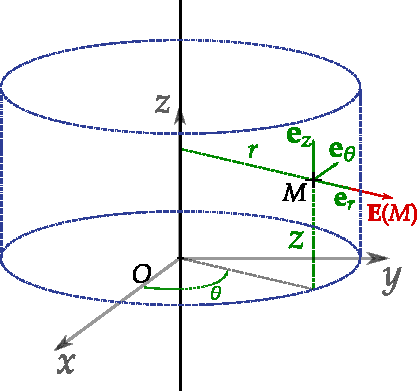
\includegraphics[scale=0.8]{fil}
	\caption{Schéma du fil chargé avec le repère cylindrique associé. 
		La surface de Gauss utilisée apparaît en tiret-pointillé bleu.}%
	\label{fig:fil}
\end{figure}
\end{corr}

\end{bibunit}

\begin{bibunit}
\graphicspath{{Chapitre_2/figure/}}
\chapter{Champ électrique dans un conducteur}
\label{chap:metaux}
\section*{Objectifs}
\begin{itemize}
	\item Comprendre comment on peut modéliser la réponse 
	  un matériau au travers d'une relation constitutive
	\item Connaître la notion de résistivité
	\item Connaître la loi d'Ohm locale
	\item Comprendre comment on peut sonder le sol grâce à la résistivité
\end{itemize}

\section*{Introduction}
\begin{figure}[]
	\centering
	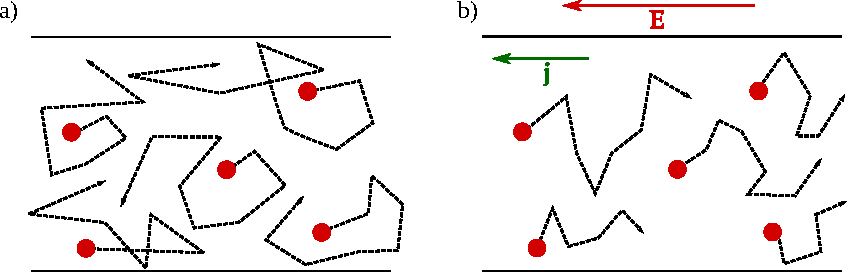
\includegraphics[width=\linewidth]{e_libre}
	\caption{Schéma du mouvement des électrons libres dans un conducteur
		 sans champ électrique (à gauche) et avec champ électrique 
	 	 (à droite). Le champ électrique conduit à un mouvement 
	 	d'ensemble qui génère un vecteur densité de courant $\mitbf{j}$.}%
	\label{fig:e_libre}
\end{figure}

Les conducteurs contiennent des \emph{électrons libres}, c'est-à-dire libres de se 
mouvoir. Ces derniers, soumis à l'agitation thermique, sont animés d'un mouvement
erratique (voir Fig.~\ref{fig:e_libre}). 
Pour générer un courant, il est nécessaire
d'exercer une force sur ces derniers, de manière à créer un mouvement d'ensemble.
Dans un circuit électrique par exemple, on impose une différence de potentiel 
entre ses bornes. Les conducteurs solides, tels que le cuivre, contiennent
un nombre important d'atomes, l'étude du mouvement d'un électron devient alors 
difficile.
Dans ce chapitre, nous allons voir comment modéliser le comportement d'un conducteur 
soumis à un champ électrique.
\section{Quelques rappels sur le courant électrique}

\begin{defn}[Courant électrique]
Un courant électrique est un mouvement de charges électriques. Il est caractérisé 
par son \textbf{intensité}, qui mesure le débit de charges électriques qui traverse
une unité de surface par unité de temps. Elle se mesure en ampères ($\ampere$)
qui correspondent à des $\coulomb \usk \reciprocal \second$ et peut-être 
positive ou négative.
\end{defn}

\begin{exemple}
	Les prises domestiques fournissent un courant dont l'intensité vaut
	$\unit{16}{\ampere}$, voire $\unit{32}{\ampere}$ pour les plaques à induction. 
	Pour une batterie de téléphone, l'intensité vaut
	$\unit{1}{\ampere}$ environ.
\end{exemple}

\begin{defn}[Vecteur densité de courant]
	En tout point de l'espace, un courant électrique est caractérisé par le vecteur 
densité de courant  
	\begin{equation}
		\vecj = n q \vecv,
		\label{eq:jnqv}
	\end{equation}
	où $q$ est la charge d'un porteur de charge ($\coulomb$), $n$ est le
	nombre de charges mobiles par unité de volume ($\rpcubic \meter$) et
	$\vecv$ la vitesse d'un porteur de charge. C'est une grandeur additive.
	L'intensité $\mathrm{d}i$
	qui traverse une surface élémentaire $\ds_P$ centrée sur le point 
	$P$ est donc donnée par 
	\begin{equation}
		\mathrm{d}i = \vecj(P) \cdot \ds_P.
	\end{equation}
	L'intensité totale $I$ traversant une surface macroscopique $\mathcal{S}$
	est donc donnée par 
	\begin{equation}
		I = \iint_\mathcal{S} \vecj(P) \cdot \ds_P.
	\end{equation}
\end{defn}

\begin{exemple}
	On considère un câble de chargeur de téléphone de section $S = \unit{1}
	{\milli \meter \squared}$ alimenté par un courant $I = \unit{1}{\ampere}$.
	Si on suppose que le courant est uniforme à l'intérieur du câble, on a
	$\vecj = I/S = \unit{10^6}{\ampere \usk \meter \squared}$. La partie 
	conductrice du câble est composée principalement de cuivre. Dans le cuivre, 
	les porteurs de charges sont des électrons avec $q = \unit{1.6 \times 10^{-19}
	}{\coulomb}$ et $n \approx \unit{10^{29}}{\rpcubic \meter}$. On peut alors remonter
	à la vitesse de dérive des électrons $v = \unit{60}
	{\micro \meter \usk \reciprocal \second}$
\end{exemple}

Le vecteur densité de courant possède une propriété intéressante en régime 
permanent.
En effet, imaginons le cas d'une sphère contenant une charge $Q$. En régime permanent,
la charge $Q$ contenue dans cette sphère est constante. Le débit total de
charge à travers la sphère est donc nulle. Le vecteur densité de courant est donc 
à flux conservatif.

\begin{defn}[Flux conservatif du vecteur densité de courant]
	En régime permanent, le flux du vecteur densité de courant $\vecj$
	à travers une surface fermée $\mathcal{S}$ est nul
	\begin{equation*}
		\oiint_\mathcal{S} \vecj \cdot \ds = 0.
	\end{equation*}
	$\vecj$ est donc à \textbf{flux conservatif}. Cette égalité peut se traduire
	sous une forme locale
	\begin{equation*}
		\grad \cdot \vecj = 0.
	\end{equation*}
\end{defn}

\begin{rem}
	La loi des n\oe{}uds en électrocinétique découle de la conservativité du
	flux du vecteur densité de courant.
\end{rem}

\section{Le modèle de Drude}
On considère dans cette partie un fil électrique de densité volumique
de porteur de charge $n$. En l'absence de champ électrique, le mouvement
des porteurs de charge est erratique. Leur vitesse est donc nulle en moyenne
et le fil n'est traversé par aucun courant. À l'instant $t=0$, il est plongé dans 
un champ électrique $\vece$ uniforme et constant. Un courant apparaît alors dans 
le fil. Dans cette partie, on cherche
à relier la densité de courant $\vecj$ parcourant le fil et le champ électrique 
$\vece$ imposé.

Expérimentalement, on constate que l'intensité du courant, après une certaine durée,
se stabilise à une valeur constante. 
À partir de l'équation~\ref{eq:jnqv}, on conclut que les 
électrons doivent atteindre une vitesse d'ensemble limite dans le fil. Pour modéliser 
ce comportement et par analogie avec la chute d'un corps, 
le physicien Paul Drude propose l'introduction d'une force de frottement 
qui s'opposerait à la mise en mouvement des électrons. Cette force de 
frottements modélise notamment la présence du réseau cristallin dans lequel évolue 
l'électron. 

On considère alors une particule de charge $q$ et de masse $m$ se déplaçant à la
vitesse $\vecv$.
Dans le référentiel du fil, supposé galiléen, cette particule est soumise à la 
force électrostatique $q\vece$ et à la force de frottement fluide $-\alpha \vecv$, 
où $\alpha$ est le coefficient de frottement (\kilogram \usk \reciprocal \second)
caractéristique du milieu. Pour simplifier le problème, 
on considère que sa vitesse est nulle en 
l'absence de champ électrique. On a donc notamment, $\vecv(t = 0) = \mitbf{0}$.
Le principe fondamental de la dynamique appliqué 
à ce porteur de charge donne

\begin{equation}
	m \dfrac{\mathrm{d}\vecv}{\dt} = q\vece - \alpha\vecv
	\iff \dfrac{d\vecv}{\dt} + \dfrac{\vecv}{\tau} = \dfrac{q\vece}{m},
\end{equation}
où $\tau = m/\alpha$ est homogène à un temps. La solution générale de cette équation
s'écrit

\begin{equation}
	\vecv(t) = \veca \exp\left(-\dfrac{t}{\tau}\right) + \dfrac{q\tau}{m}\vece,
\end{equation}
où $\veca$ est une constante d'intégration. Avec la condition initiale,
$\vecv(t=0) = \mitbf{0}$, on obtient

\begin{equation}
	\vecv(t) = \dfrac{q \tau}{m} 
	           \left[1 - \exp\left(\dfrac{-t}{\tau}\right)\right]\vece.
\end{equation}
$\tau$ apparaît alors comme étant le temps de relaxation de la vitesse du  
porteur de charge. Dès que $t$ est plus grand que quelques $\tau$, 
le porteur de charge a atteint la vitesse limite

\begin{equation}
	\vecv_\mathrm{lim} = \dfrac{q \tau}{m} \vece = \dfrac{q}{\alpha} \vece.
\end{equation}
On peut alors établir une relation directe entre entre la densité volumique
de courant $j$ parcourant le fil et le champ électrique $\vece$ imposé sur ce dernier,
en multipliant cette vitesse par $nq$ (voir Éq.~\ref{eq:jnqv})

\begin{equation}
	\vecj = \dfrac{nq^2\tau}{m} \vece = \gamma \vece,
\end{equation}
où $\gamma$ est la conductivité électrique du matériau. On définit de même
la résistivité $\rho$

\begin{equation}
	\rho = \dfrac{1}{\gamma},
\end{equation}
qui s'exprime en $\ohm \reciprocal \meter$.

\begin{defn}[Loi d'Ohm locale]
	La loi d'Ohm locale est une relation constitutive, elle est donc spécifique
	au conducteur. Elle permet de décrire leur réponse à un champ électrique.
	Un conducteur soumis à un champ électrique $\vece$ est traversé
	par une densité volumique de courant $\vecj$ telle que 
	\begin{equation}
		\vecj = \gamma \vece.
	\end{equation}
	$\gamma$ est la conductivité du conducteur. Elle est caractéristique du
	matériau considéré et s'exprime en siemens par mètre ($\siemens \usk 
	\reciprocal \meter$). Elle mesure la facilité d'un courant à parcourir 
	un matériau. En l'absence de champ électrique, le courant à l'intérieur
	d'un conducteur est donc nul. C'est une grandeur qui dépend de la température. 
	Le tableau~\ref{tab:conductivite} donne la conductivité de matériaux usuels.
\end{defn}

\begin{rem}
	On remarque que le champ électrique est toujours orienté dans la même
	direction que le vecteur de densité volumique de courant.
\end{rem}

\begin{table}
	\centering
	\caption{Ordre de grandeur de conductivités de matériaux usuels. Pour le
		 cuivre et l'eau, les valeurs données sont celles obtenues 
	 	 à température ambiante.}
	\begin{tabular}{l|c}
		\textbf{Matériau} & \textbf{Conductivité électrique} 
		($\siemens \usk \reciprocal \meter$)\\ \hline
		Eau distillée 	 & $1.0 \times 10^{-6}$ à $\unit{300}{\kelvin}$ \\[0.5em]
		Cuivre   & $5.9 \times 10^7$ à $\unit{300}{\kelvin}$\\[0.5em]
		Basalte   & $10^{-5} - 0.5$ \\[0.5em]
		Grès     & $10^{-3} - 1$\\[0.5em]
		Argile   & $10^{-2} - 1$\\[0.5em]
		Graphite & $5 \times 10^{2} - 10^4$\\ \hline
	\end{tabular}
	\label{tab:conductivite}
\end{table}

\section{Sondage résistif}
La notion de résistivité est particulièrement intéressante en sciences de la 
Terre. Elle est notamment utilisée pour sonder le sol à la recherche de minerai.
Comme le montre le Tableau~\ref{tab:conductivite}, la résistivité des minerais tels que
le cuivre est bien plus élevée que celle des roches qui le contiennent. Ce contraste
de résistivité permet alors de les localiser en utilisant par exemple le montage
à 4 électrodes que nous allons présenter.

\subsection{Potentiel électrique d'une électrode}
\begin{figure}[]
	\centering
	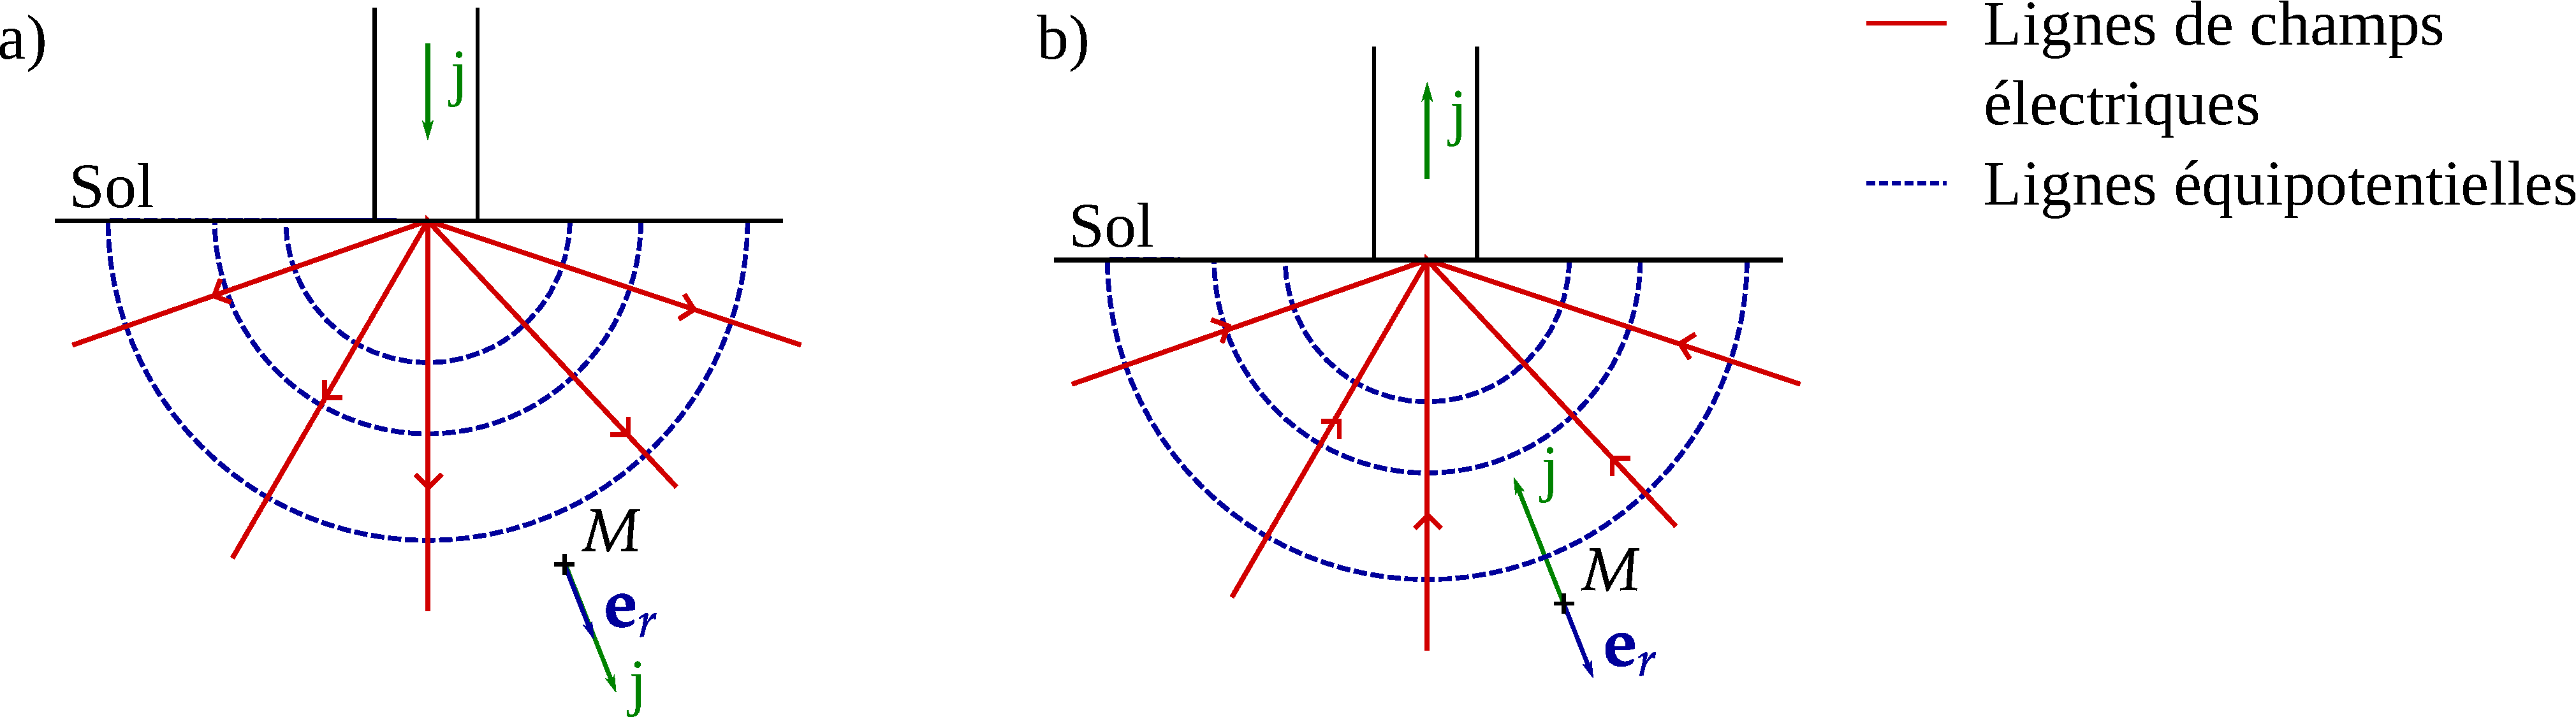
\includegraphics[scale=1]{electrode}
	\caption{Schéma d'une électrode émettrice (à gauche) et réceptrice (à droite).
		 L'électrode est parcourue
	par une densité volumique de courant $\vecj$. Elle génère dans le sol
	un champ électrique $\vece$ dont on a représenté les lignes de champs en rouge.
	Quelques lignes équipotentielles du potentiel $V$ résultant de ce champ
	sont dessinées sous la forme de lignes bleues pointillées.}%
	\label{fig:electrode}
\end{figure}

On considère une électrode de section $S$ parcourue par un courant d'intensité $I$ 
et de densité volumique de courant $\vecj$ plantée dans un sol uniforme de résistivité
$\rho$. (voir Fig~\ref{fig:electrode}a). Le point de contact de l'électrode avec le sol
agit comme une source de courant en injectant un courant d'intensité $I$ dans
ce dernier. Le système présente une symétrie sphérique, $\vecj$ ne dépend donc 
que de la distance à l'électrode et est porté par le vecteur radial $\er$.
La densité de courant volumique $\vecj$ en un point $M$ de l'espace à une
distance $r$ de la source est donnée par

\begin{equation}
	\vecj(r) = \dfrac{I}{2 \pi r^2} \er,
\end{equation}
où $2 \pi r^2$ est la surface de la demi-sphère de rayon $r$.
Cette électrode génère donc dans le sol un champ électrique $\vece$ relié
à $\vecj$ par la loi d'Ohm locale

\begin{equation}
	\vece(r) = \rho \vecj(r) = \dfrac{\rho I}{2 \pi r^2} \er.
\end{equation}
Le potentiel électrostatique $V$ en un point $M$ de l'espace est donc déduit
en utilisant la relation liant le champ électrique au potentiel électrostatique

\begin{equation}
	\vece (r) = -\grad(V) = -\dfrac{\mathrm{d}V}{\dr}(r) \er 
	\iff V(r) = \dfrac{\rho I}{2 \pi r}
	\label{eq:potentiel}
\end{equation}
en fixant le potentiel électrostatique nul en l'infini.
Le potentiel électrostatique dépend donc directement de la résistivité du milieu
considéré.

\subsection{Le montage à 4 électrodes}
\begin{figure}[]
	\centering
	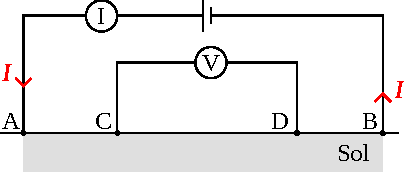
\includegraphics[]{4electrode}
	\caption{Schéma du montage à 4 électrodes. Le générateur fournit un courant
		 d'intensité $I$ qui se distribue dans le sol en A et ressurgit en 
	 	 B. Un voltmètre et un ampèremètre permettent de mesurer respectivement
		 la tension
	 	 entre les points D et C et l'intensité $I$. Les électrode D
	 	 et C ne sont parcourues par aucun courant.}%
	\label{fig:4electrode}
\end{figure}
On présente maintenant le montage à 4 électrodes qui permet de remonter à la 
résistivité $\rho$ du sol. On considère ici un sol uniforme.
La Figure~\ref{fig:4electrode} fourni un schéma 
du montage. D'après l'équation~\ref{eq:potentiel}, les électrodes en A et B 
génèrent un potentiel en C donné par
\begin{equation*}
	V_C^A = \dfrac{\rho I}{2 \pi |AC|} \quad \mathrm{et} \quad
	V_C^B = -\dfrac{\rho I}{2 \pi |BC|}.
\end{equation*}
Le signe $-$ dans l'expression de $V_C^B$ provient de l'orientation de $\vecj$ 
au point D (voir Fig.~\ref{fig:electrode}b). Finalement, le potentiel au point $C$
résulte de la superposition de ces deux potentiels
\begin{equation*}
	V_C = V_C^A + V_C^B = \dfrac{\rho I}{2 \pi}
	                    \left(\dfrac{1}{|AC|} - \dfrac{1}{|BC|}\right).
\end{equation*}
De même, le potentiel de l'électrode au point D est donnée par
\begin{equation*}
	V_D = \dfrac{\rho I}{2 \pi}
	      \left(\dfrac{1}{|AD|} - \dfrac{1}{|BD|}\right).
\end{equation*}
La différence de potentiel $\Delta V$mesurée par le voltmètre est donc donnée par 
\begin{equation*}
	\Delta V = V_C - V_D = \dfrac{\rho I}{2 \pi}\left(
		\dfrac{1}{|AC|} - \dfrac{1}{|BC|}
	- \dfrac{1}{|AD|} + \dfrac{1}{|BD|} \right)
\end{equation*}
En dehors de la résistivité $\rho$, toutes les autres grandeurs apparaissant dans
cette égalité sont connues. On peut donc remonter à la résistivité du sol
\begin{equation}
	\rho = \dfrac{2 \pi \Delta V}{I}\left(
		\dfrac{1}{|AC|} - \dfrac{1}{|BC|}
	- \dfrac{1}{|AD|} + \dfrac{1}{|BD|} \right)^{-1}
\end{equation}
Certaines configurations d'électrodes permettent d'obtenir une formule finale
simple. On peut citer par exemple la configuration de Wenner, pour laquelle
$|AC| = |DB| = a$ et $|CB| = |AD| = 2a$. La formule précédente devient alors
\begin{equation}
	\rho = 2 \pi a \dfrac{V}{I}.
\end{equation}

\subsection{Distribution de courant}
\begin{figure}[]
	\centering
	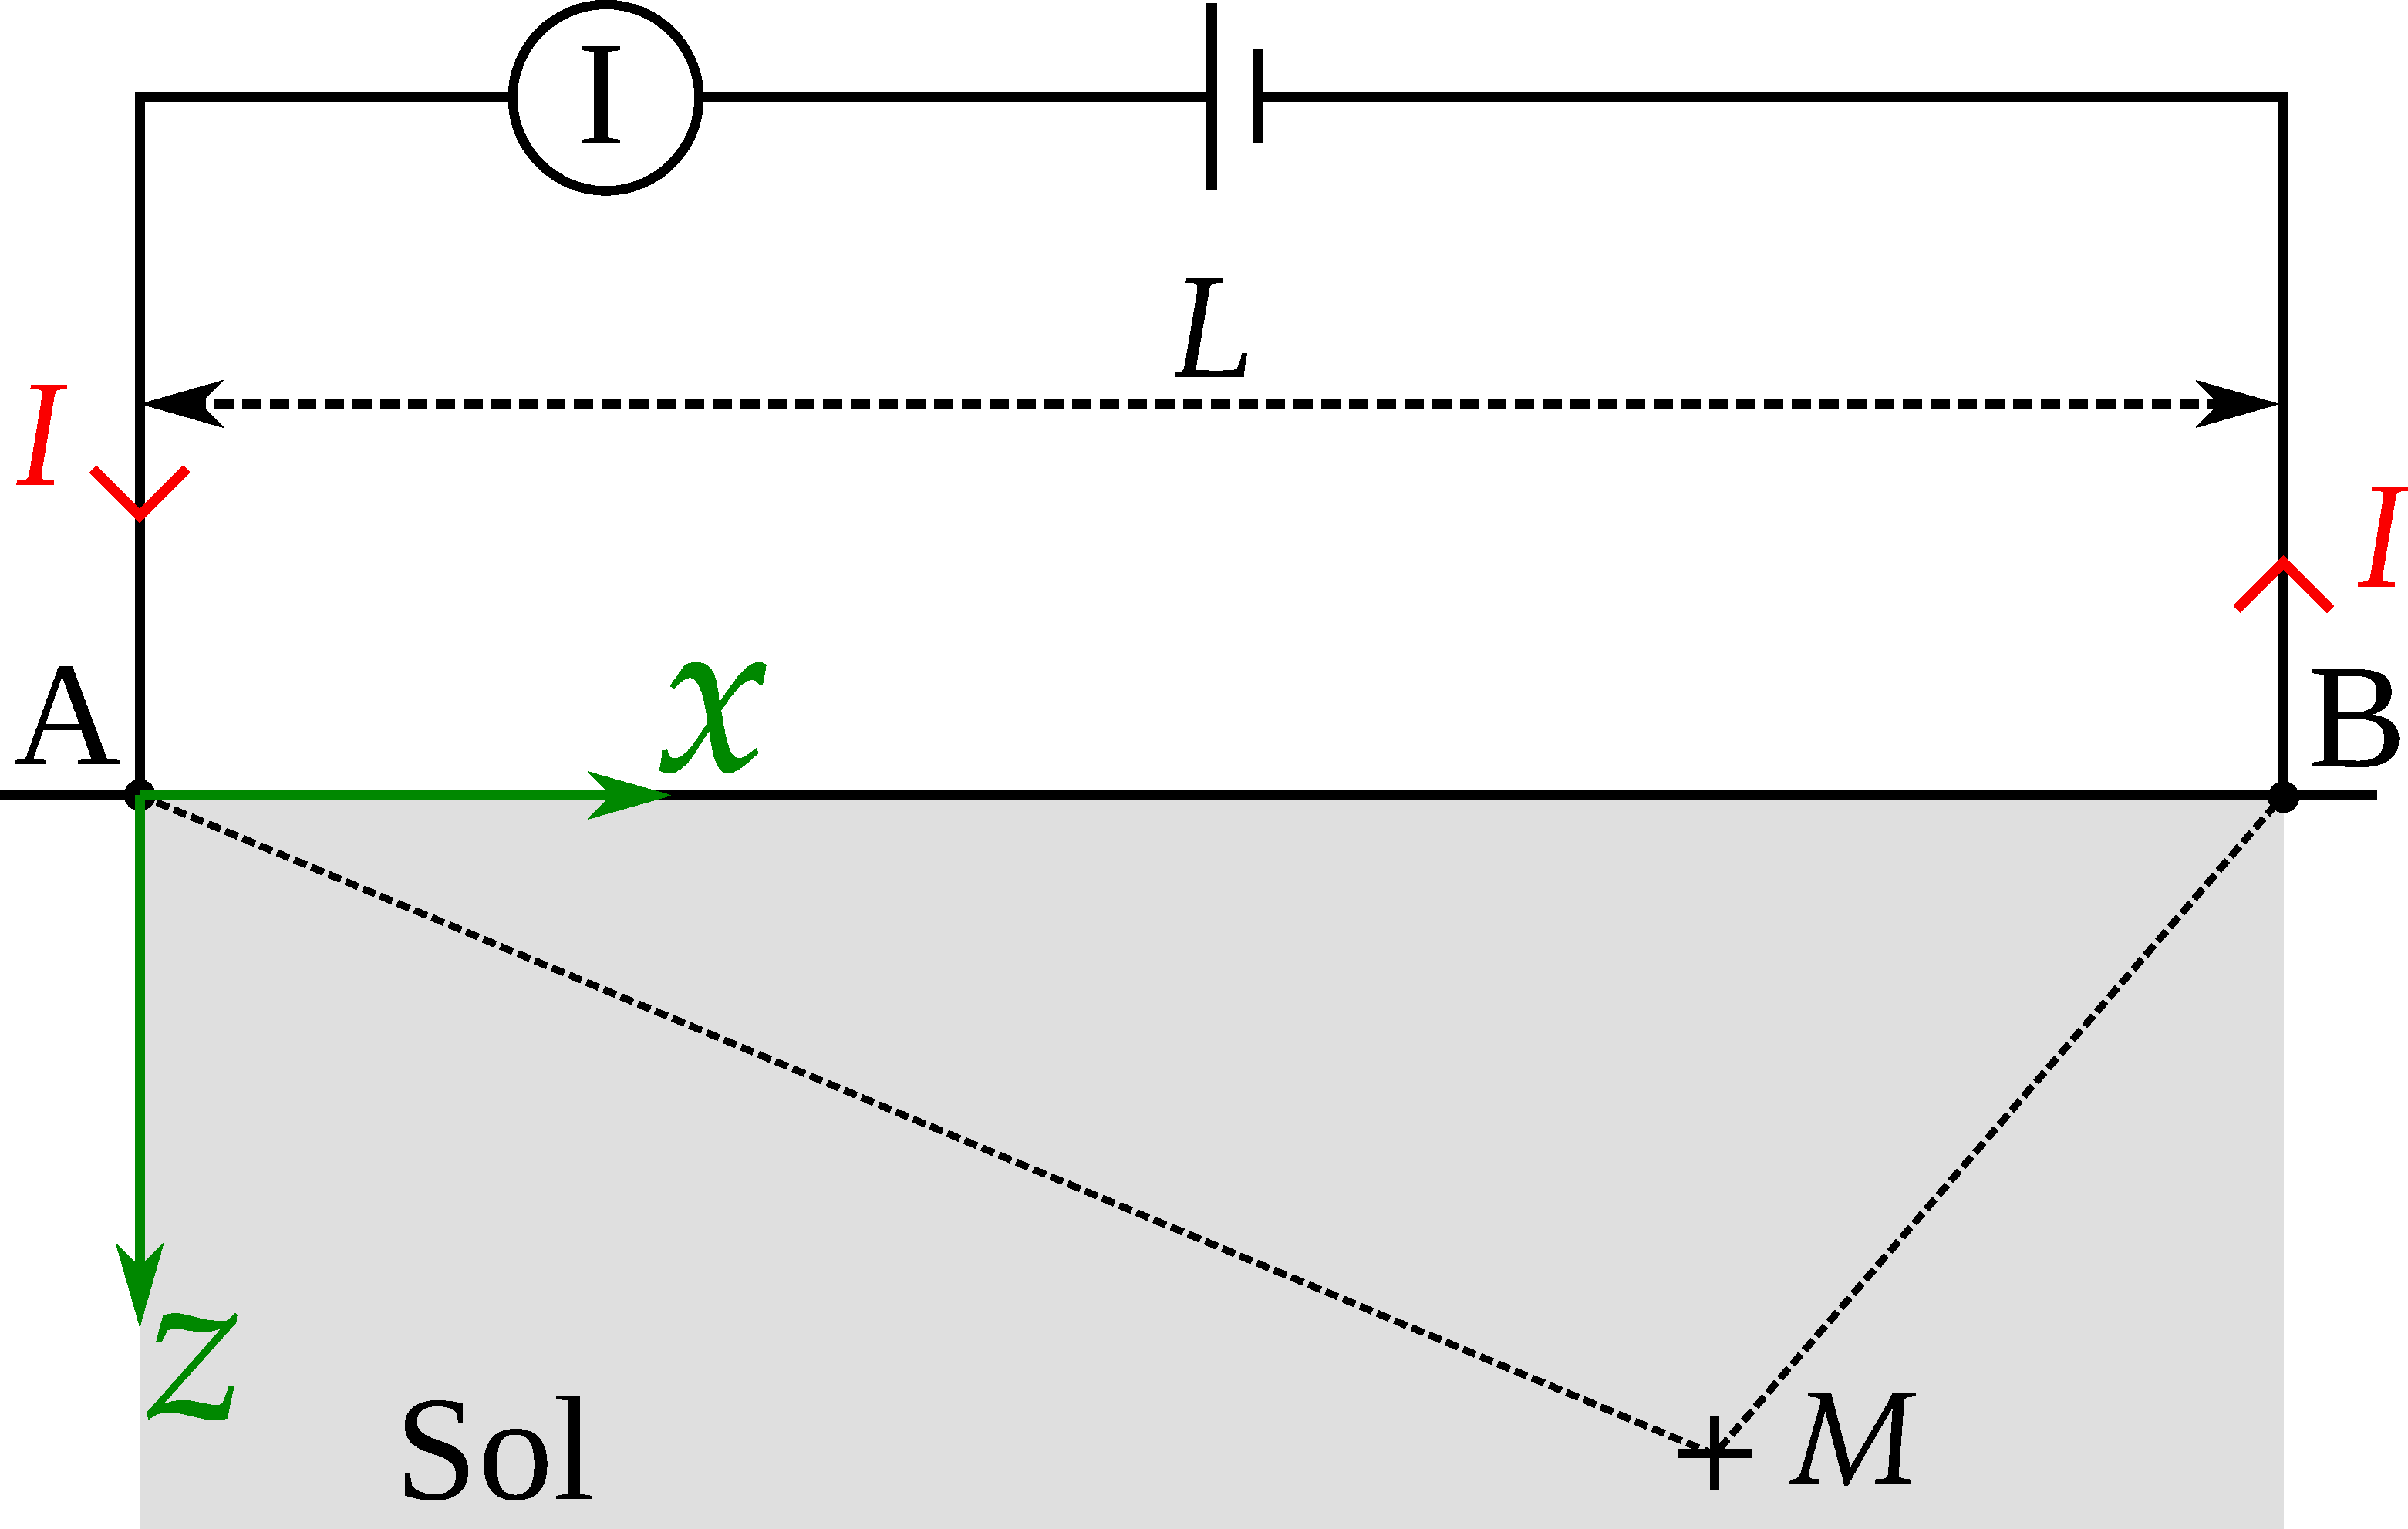
\includegraphics[]{penetration_courant}
	\caption{Paire d'électrodes alimentées par un courant d'intensité $I$
		 et séparées par une distance $L$.}%
	\label{fig:penetration_courant}
\end{figure}
On s'intéresse maintenant à la distribution de courant générée dans le sol
par une paire d'électrodes émettrice-réceptrice. On cherche à connaître la 
profondeur maximale que permet de sonder une paire d'électrodes. 

On considère donc une paire d'électrodes A et B alimentées par un courant d'
intensité $I$ et séparées 
par une distance $L$ (voir Fig.~\ref{fig:penetration_courant}). 
Le sol est un demi-espace infini de résistivité $\rho$ uniforme. 
On se place dans un repère cartésien $(O, \ex, \ey, \ez)$. Un point $M$ de l'espace
est donc repéré par ses coordonnées $(x, y, z)$.

La paire d'électrodes génère au point $M$ un champ électrostatique $\vece$ dont
la composante selon $\ex$ vaut
\begin{equation*}
	E_x(M) = - \dfrac{\partial}{\ddx}\left[\dfrac{\rho I}{2 \pi} 
	\left( \dfrac{1}{|AM|} - \dfrac{1}{|BM|}\right)\right],
\end{equation*}
où $|AM| = \sqrt{x^2 + y^2 + z^2}$ et $|BM| = \sqrt{(L - x)^2 + y^2 + z^2}$.
On a alors
\begin{equation*}
	E_x(M) = \dfrac{\rho I}{2 \pi}\left(\dfrac{x}{|AM|^3} 
	    + \dfrac{L - x}{|BM|^3}\right).
\end{equation*}
On peut alors aboutir à la composante $j_x$ de la densité volumique de courant
$\vecj$ en utilisant la loi d'Ohm
\begin{equation}
	j_x(M) = \dfrac{E_x}{\rho} = \dfrac{I}{2 \pi}\left(\dfrac{x}{|AM|^3} 
	    + \dfrac{L - x}{|BM|^3}\right).
\end{equation}

On s'intéresse maintenant au cas où le point $M$ appartient au plan médian $
x = L/2$ aux
deux électrodes. Dans ce cas particulier, $j_x$ vaut
\begin{equation*}
	j_x(M) = \dfrac{IL}{2 \pi \left[(L/2)^2 + y^2 + z^2\right]^{3/2}}.
\end{equation*}
L'intensité $\mathrm{d}I_x$ du courant traversant la surface 
élémentaire $\dy\dz \ex$ centré en $M$ s'écrit
\begin{equation*}
	\mathrm{d}I_x = \vecj(M) \cdot \dy\dz\ex = j_x(M) \dy\dz
	    = \dfrac{IL}{2 \pi \left[(L/2)^2 + y^2 + z^2\right]^{3/2}} \dy\dz.
\end{equation*}
La fraction de courant qui traverse une section du plan médian jusqu'à une 
profondeur $p$ est alors donnée par
\begin{equation*}
	\dfrac{I_x}{I}(p) = \int_{y=-\infty}^{y=\infty} \int_{z=0}^{z=p}
	\dfrac{IL}{2 \pi \left[(L/2)^2 + y^2 + z^2\right]^{3/2}} \dy\dz.
\end{equation*}
Comme 
	\begin{equation*}
		\int_{y=-\infty}^{y=\infty} \dfrac{\dy}{
			\left[(L/2)^2 + y^2 + z^2\right]^{3/2}} = 
		\dfrac{2}{\left[(L/2)^2 + z^2\right]^{3/2}},
	\end{equation*}
l'équation précédente devient
\begin{equation*}
	\dfrac{I_x}{I}(p) = \int_{z=0}^{z=p}
	\dfrac{IL}{\pi \left[(L/2)^2 + z^2\right]} \dz.
\end{equation*}
On obtient alors finalement
\begin{equation}
	\dfrac{I_x}{I}(p) = \dfrac{2}{\pi}\arctan\left(\dfrac{2p}{L}\right).
\end{equation}

\begin{figure}[]
	\centering
	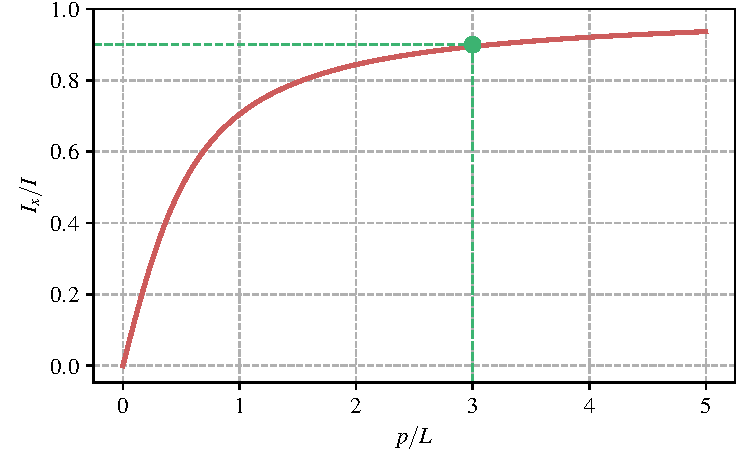
\includegraphics[scale=0.6]{arctan}
	\caption{Intensité relative traversant une section de sol située 
		en $x = L/2$ jusqu'à la profondeur
	$p$ en fonction du rapport de $p$ sur la distance inter-électrode $L$.
	Le point vert correspond au point particulier $(3, 0.9)$.}%
	\label{fig:arctan}
\end{figure}
Sur la Figure~\ref{fig:arctan}, on a tracé l'évolution de l'intensité relative traversant
une section de sol située en $x = L/2$ 
jusqu'à la profondeur $p$ en fonction du rapport de $p$ sur 
la distance inter-électrode $L$. 
On remarque que $90\,\%$ de l'intensité $I$ traverse une section de sol s'étendant
jusqu'à la profondeur $3L$. En augmentant la distance $L$ entre les deux électrodes,
on peut alors sonder le sol à une profondeur plus élevée.

\subsection{Résistivité apparente}
\begin{figure}[]
	\centering
	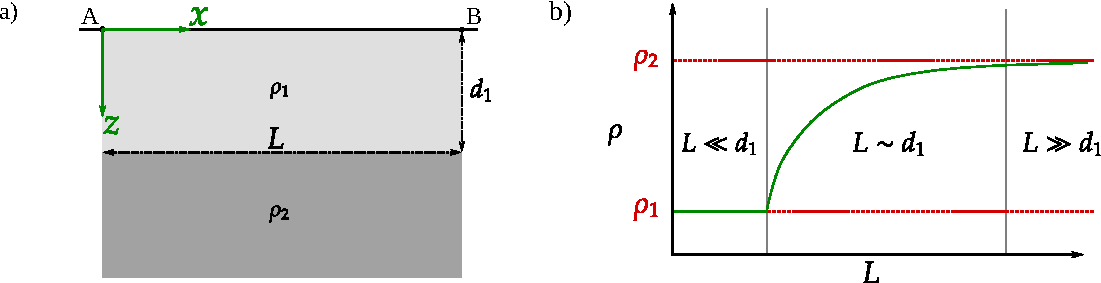
\includegraphics[scale=0.65]{resistivite_apparente}
	\caption{Mesure de la résistivité d'un sol bicouche avec 2 électrodes
		avec le montage à gauche et l'évolution schématique de la résistivité
		apparente $\rho$ avec la distance $L$ entre les électrodes à droite.
		Les deux électrodes sont séparées d'une distance $L$ et 
		alimentées par un courant d'intensité $I$. La première couche 
		présente une épaisseur $d_1$ et une résistivité $\rho_1$, tandis
		que la seconde couche présente une résistivité 
		$\rho_2$ avec $\rho_1 < \rho_2$.}%
	\label{fig:apparente}
\end{figure}
Nous n'avons pour l'instant considéré que le cas idéal d'un sol de résistivité 
uniforme $\rho$. Dans ce cas bien précis, la méthode des 4 électrodes permet de
déterminer la résistivité exacte de ce dernier. 

En réalité, la résistivité d'un sol est une fonction complexe de l'espace qui résulte 
de sa composition, de sa température et d'autres paramètres physiques. 
La résistivité mesurée par la méthode des 4 électrodes est alors
qualifiée d'\emph{apparente}. Cette mesure donne néanmoins des informations utiles
sur la structure du sol sondé.

Pour bien illustrer cela, on considère le cas d'un sol composé de deux couches
de résistivités uniformes $\rho_1$ et $\rho_2$, avec $\rho_2 > \rho_1$. La couche $1$ 
s'étend sur une épaisseur $d_1$ (voir Fig.~\ref{fig:apparente}(a)). 
Pour simplifier le problème,
on décide de sonder ce sol à l'aide de deux électrodes séparées d'une distance $L$
et alimentées par un courant d'intensité $I$. La résistivité mesurée va alors dépendre de
la distance entre les deux électrodes (voir Fig.~\ref{fig:apparente}(b))
\begin{enumerate}
	\item lorsque $L \ll d_1$, seule la première couche de sol est sondée.
	  La résistivité mesurée sera alors proche de $\rho_1$.
	\item lorsque $L \gg d_1$, la majeure partie de l'intensité traverse la seconde
	  couche de sol. La résistivité mesurée tend vers $\rho_2$.
	\item lorsque $L \sim d_1$, les deux couches sont sondées de manière équivalente.
	  La résistivité mesurée se situe entre $\rho_1$ et $\rho_2$.
\end{enumerate}
En faisant varier la distance $L$ entre les deux électrodes, on est alors capable d'avoir
une carte schématique de la résistivité du sol sondé et donc de connaître la 
composition de ce dernier. 

\nocite{*}
\putbib[Chapitre_2/metaux]
\begin{td}{Champ électrique dans un conducteur}
\exercice{Effet de peau}
	Le demi-espace $x < 0$ est rempli d'air tandis que le demi-espace
	$x > 0$ est constitué d'un métal. Lorsqu'une onde électromagnétique 
	venant de l'air se réfléchit sur le métal, le métal est le siège de courants
	volumiques de la forme 
	\begin{equation*}
	\vecj = j_0 \exp\left(\dfrac{-x}{\delta}\right)\ey,
	\end{equation*}
	où $j_0$ et $\delta$ sont des constantes.
	\begin{exlist}
		\item Donner la dimension de $j_0$ et de $\delta$. À quoi correspond
		  $\delta$ ?
		\item $\delta$ est appelé l'épaisseur de peau. Elle dépend de
		  la conductivité en régime stationnaire $\sigma$ du matériau considéré
		  et de la pulsation de l'onde électromagnétique $\omega$
		  \begin{equation*}
			  \delta = \sqrt{\dfrac{2}{\mu_0 \omega \sigma}},
		  \end{equation*}
		  où $\mu_0 = \unit{4 \pi \times 10^{-7}}{\kilogram \usk \meter
		  \usk \rpsquare \second \usk \rpsquare \ampere}$ 
		  est la perméabilité magnétique du vide.
		  Vérifier l'homogénéité de cette expression.
		\item Déterminer $\delta$ dans le cas d'un gisement de pyrrhotite
		  de résistivité $\rho = \unit{5 \times 10^{-5}}{\ohm \usk
		  \meter}$ pour 2 méthodes de prospection différentes utilisant des
		  ondes électromagnétiques
		  \begin{exlist}
			  \item induction électromagnétique ($f = \unit{1}{\kilo \hertz}$)
			  \item radar ($f = \unit{100}{\mega \hertz}$)
		 \end{exlist}
		 Ces méthodes permettent-elles de détecter le gisement s'il est enfoui
		 sous un sol de $\unit{3}{\meter}$ d'épaisseur et ayant une résistivité de 
		 $\unit{100}{\ohm \usk \meter}$?
	 	\item L'\oe{}il humain perçoit des ondes électromagnétiques dont la
		  fréquence est située entre $400$ et $\unit{780}{\tera \hertz}$ 
		  environ. Quelle est la valeur de $\delta$ pour ces fréquences et pour
		  le cuivre? Quelle propriété de ce dernier cette valeur traduit-elle ?
	\end{exlist}

\newpage

\exercice{Contamination d'un aquifère}
	De l'eau de mer contamine un aquifère qui sert de source d'eau potable à 
	une ville côtière. Les mesures suivantes de résistivité apparente ont été
	réalisées pour différentes distances inter-électrodes avec la méthode de 
	Wenner pour déterminer la profondeur de la contamination.
	
	\begin{equation*}
	\begin{array}{l l| l l| l l} \\
		a (\meter) & \rho (\ohm \usk \meter) & a (\meter) & 
		\rho (\ohm \usk \meter) &a(\meter) & \rho (\ohm \usk \meter) \\ \hline
		10	& 29.0	& 140	& 19.8	& 280	& 8.7 \\
		20	& 28.9	& 160	& 18.0	& 300	& 7.8 \\
		40 	& 28.5	& 180	& 16.3	& 320	& 7.1 \\
		60	& 27.1  & 200	& 14.5	& 340	& 6.7 \\
		80	& 25.3	& 220	& 12.9	& 360	& 6.5 \\
		100	& 23.5	& 240	& 11.3	& 400	& 6.4 \\
		120	& 21.7	& 260	& 9.9	& 440	& 6.4 \\
	\end{array}
	\end{equation*}
	
	\begin{exlist}
		\item Tracer l'évolution de la résistivité apparente $\rho$ 
		  en fonction de la distance inter-électrode.
		\item Combien de couches différentes pouvez-vous identifier 
		  grâce à cette courbe ? Quelle est leur résistivité respective? 
		  À quelle couche correspond à l'eau salée ?
	  \item Identifier la courbe de résistivité apparente de la figure~\ref{fig:aquiferes}
	    qui correspond au problème. Tracer la résistivité apparente 
	    normalisée par la résistivité de la première 
	    couche en fonction de la distance inter-électrode normalisée pour 
	    différentes valeurs de $d$.
	    Estimer la profondeur de l'interface 
	    aquifère-eau salée. 	
	    \end{exlist}



\begin{figure}[h!]
	\centering
	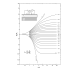
\includegraphics[scale=1.3]{aquiferes}
	\caption{Courbes caractéristiques de résistivité apparente normalisée pour un sol
		 bicouche en fonction de la distance relative inter-électrode 
		 pour le montage de Wenner. Les
	 	notations sont précisées dans la figure. L'image est extraite de 
		\cite{Lowrie2007}}%
	\label{fig:aquiferes}
\end{figure}

\exercice{Le condensateur plan}
On considère un condensateur plan composé de deux plaques conductrices infinies,
parallèles et séparées par une distance $a$. La
première plaque est chargée positivement avec une densité surfacique de charge
$\sigma$, tandis que la deuxième est chargée négativement avec une densité 
surfacique de charge $-\sigma$.

On cherche à déterminer le champ électrique généré par les deux plaques chargées.

\begin{exlist}
	\item Réaliser un schéma du système et choisir un repère adapté.
	\item Quelle est la direction et le sens du champ électrique en un point
	  situé à l'intérieur des deux plaques ?
	\item Étudier les symétries et les invariances du système. 
	\item En appliquant le théorème de Gauss aux trois surfaces suivantes,
	  	  	\begin{exlist}
			\item un cube de section $S$ inclus entre les deux plaques 
			  et situé entre les abscisses $a_1$ et $a_2$,
			\item un cube de section $S$ à l'extérieur des deux plaques
			  entre les abscisses $b_1$ et $b_2$,
			\item un cube de section $S$ contenant une partie 
			  de la plaque $1$ situé entre les abscisses $c_1$ et
			  $c_2$,

		\end{exlist}
	déterminer l'expression du champ électrique généré par les deux plaques
	en tout point de l'espace.
\end{exlist}
\end{td}



\section{Corrections}
\begin{corrige}
	\begin{enumerate}
		\item Une exponentielle est sans dimension, \fbox{$j_0$ s'exprime donc en 
			$\ampere \usk \rpsquare \meter$.}
			L'argument à l'intérieur d'une fonction est toujours sans
			dimension. \fbox{$\delta$ est donc homogène à une longueur.}
			La fonction $\exp\left(-\dfrac{x}{\delta}\right)$
			tend rapidement vers $0$. $\delta$ correspond donc à la
			profondeur de pénétration de $\vecj$, et donc de 
			l'onde électromagnétique, dans le conducteur.
		\item $\omega$ s'exprime en $\rad \usk \reciprocal \second$ et  
		  $\sigma$ s'exprime en $S \usk \reciprocal \meter$, c'est-à-dire 
		  en $\ampere \squared \usk \cubic \second \usk \reciprocal \kilogram
		  \usk \rpcubic \meter$. Le radian est une "fausse" unité car il
		  correspond au rapport de deux longueurs. Le produit $\mu_0
		  \omega \sigma$ est donc homogène à l'inverse du carré d'une longueur.
		  $\delta$ est donc bien homogène à une longueur.
		\item  On cherche à savoir ici si l'onde électromagnétique
		   plonge assez loin dans le sol pour atteindre le gisement de 
		   pyrrhotite. L'épaisseur de peau vaut dans les deux cas
		   \begin{enumerate}
			   \item $\sqrt{\dfrac{2 \times 100}{4 \pi \times 10^{-7} 
			    \times 1 \times 10^3 \times 2\pi}}
			  = \unit{0.16}{\kilo \meter}$
			\item $\sqrt{\dfrac{2 \times 100}{4 \pi \times 10^{-7} 
			    \times 1 \times 10^8 \times 2\pi}}
			  = \unit{50}{\centi \meter}$
		  \end{enumerate}
		  Le radar ne permettrait donc pas de détecter le gisement.

   	\item Pour le cuivre à température ambiante, $\sigma \approx 
          \unit{5.9 \times 10^7}{\siemens \usk \reciprocal \meter}$. 
	  Dans ce cas, $\delta \approx \unit{10}{\nano \meter}$, expliquant ainsi
	  l'opacité du cuivre.
	\end{enumerate}
\end{corrige}

\begin{corrige}
	\begin{enumerate}
		\item Voir figure~\ref{fig:aquiferes_corr}a.
		\item \fbox{On distingue deux couches de résistivités respectives 
		  $\rho_1 = \unit{29.0}{\ohm \usk \meter}$ et $\rho_2 =
	  \unit{6.4}{\ohm \usk \meter}$.} L'eau salée a une résistivité plus faible
		  que l'eau douce. La couche la plus profonde correspond donc à l'eau salée.
		\item Dans notre exercice, $k \approx -0.6$. La courbe qui nous intéresse
		  est donc celle possédant le même $k$ dans la 
		  figure~\ref{fig:aquiferes}. Cette courbe passe notamment 
		  par le point $(2, 0.5)$. Pour déterminer la profondeur de 
		  l'interface eau douce - eau salée, on trace la résistivité apparente
		  normalisée en fonction de la distance inter-électrodes normalisée
		  pour différentes valeur de $d$ (voir Fig.~\ref{fig:aquiferes_corr}b).
		  \fbox{On en déduit que $d$ est ici de l'ordre de $\unit{100}{\meter}$.}
	\end{enumerate}
\end{corrige}

\begin{figure}[h!]
	\centering
	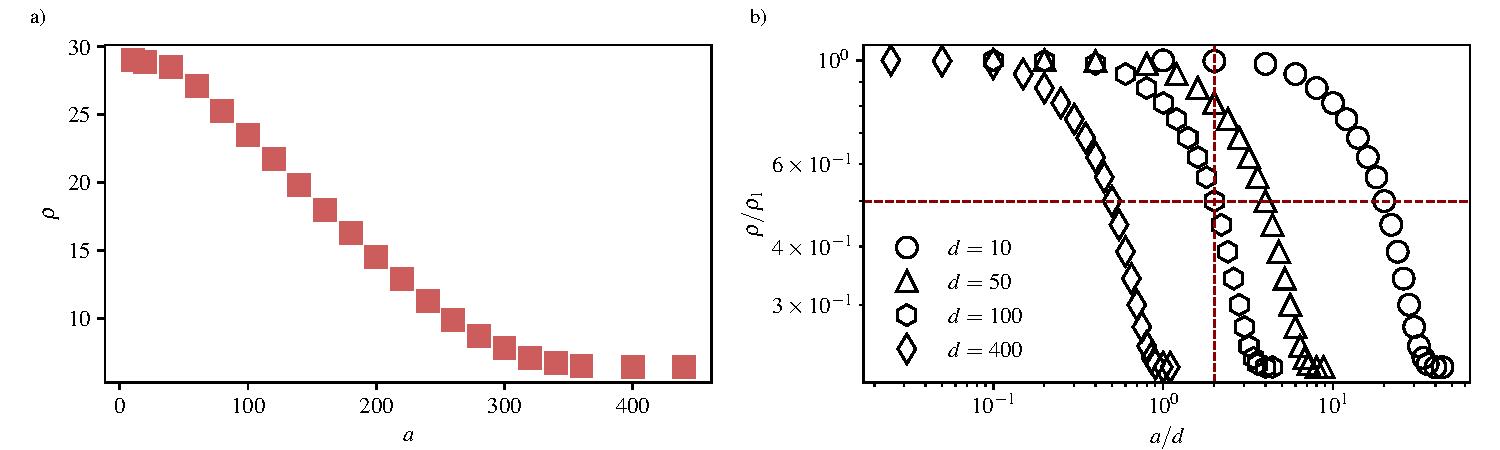
\includegraphics[width=0.8\linewidth]{aquiferes_corr}
	\caption{Résistivité apparente $\rho$ mesurée en fonction de la distance
	         inter-électrodes $a$ à gauche. Résistivité apparente normalisée
	 	 par la résistivité de la couche $1$ en fonction de la distance 
	 	inter-électrodes normalisée par l'épaisseur de la couche $1$
		à droite pour différentes valeurs de $d$. Sur le panel de 
		droite, les lignes en tiret se croisent au point $(2, 0.5)$.}%
	\label{fig:aquiferes_corr}
\end{figure}
\begin{corrige}
\begin{enumerate}
	\item Voir la figure.~\ref{fig:condensateur}
	\item Nous savons que le champ électrostatique $\vece$ est lié au potentiel
	      électrostatique $V$ par la relation
	      \begin{equation*}
		      \vece = - \grad(V).
	      \end{equation*}
	      Le champ électrique est donc dirigé des potentiels les plus élevés 
	      aux potentiels les plus faibles. La plaque $1$ étant chargée positivement
	      et la plaque $2$ négativement, \fbox{$\vece$ en un point situé à l'intérieur des
      plaques est dirigé de la plaque $1$ à la plaque $2$.}
      \item Dans un repère cartésien, la forme générale du champ électrique $\vece$ 
	    en un point $M$ de l'espace de coordonnée $(x, y, z)$ est la suivante
	    \begin{equation*}
		    \vece(M) = E_x(x, y, z)\ex + E_y(x, y, z)\ey + E_z(x, y, z)\ez.
	    \end{equation*}
	    Pour simplifier cette expression, on commence par étudier les invariances de la
	    distribution de charge générant le champ électrique $\vece$
	    \begin{itemize}
		    \item les deux plaques étant infinies, le système est invariant
			  par translation selon l'axe $\ez$. $\vece$ ne dépend pas
			  de $z$,
		    \item le système est invariant par translation selon $\ey$.
			  $\vece$ ne dépend pas de $y$.
	   \end{itemize}
	   \fbox{$\vece$ ne dépend donc que de $x$}.

	   On étudie maintenant les symétries de cette distribution de charge 
	   en considérant un point $M$ quelconque de l'espace
	   \begin{itemize}
		   \item le plan $(M, \ex, \ey)$ est un plan de symétrie de 
			 la distribution de charges. $\vece(M)$ doit donc
			 appartenir à ce plan,
		   \item le plan $(M, \ex, \ez)$ est un plan de symétrie de la
			 distribution de charge. $\vece(M)$ doit donc appartenir
			 à ce plan.
	 \end{itemize}
	 $\vece(M)$ doit appartenir aux plans $(M, \ex, \ey)$ et $(M, \ex, \ez)$, 
	 \fbox{il est donc colinéaire à $\ex$}. On a finalement
	 \begin{equation}
		 \vece(M) = E(x)\ex,
	 \end{equation}
	 en tout point de l'espace $M$. Cette forme simple est propice à 
	 l'utilisation du théorème de Gauss.

 	 \item On applique donc le théorème de Gauss aux trois surfaces fermées
	       proposées
	       \begin{enumerate}
		       \item La surface fermée ne contient aucune charge, le flux
			     de $E$ à travers cette surface est donc nul. On a donc
			     $E(a_1) = E(a_2)$. Comme nous n'avons imposé aucune condition
			     sur le placement de la surface (hormis le fait
			     qu'elle soit incluse entre les deux plaques), on peut
			     conclure que \fbox{$\vece$ est uniforme entre les deux plaques.}
		       \item Par un raisonnement analogue, on conclut que $\vece$
			     est uniforme à l'extérieur des plaques. \fbox{$\vece$ doit
			     donc être nul à l'extérieur des plaques} pour éviter la génération
		     par ce système d'une énergie infinie.
	     		\item La surface contient la charge $\sigma S$. Le théorème de
			Gauss donne donc
			\begin{equation*}
			E(c_1) - E(c_2) = \dfrac{\sigma}{\epsilon_0}.
			\end{equation*}
			$E(c_2)$ étant nul on obtient finalement
			\begin{equation*}
				E(c_1) = \dfrac{\sigma}{\epsilon_0}
			\end{equation*}
			\begin{defn}[Relation de continuité du champ électrostatique]
				Au passage d'une surface possédant une densité surfacique de
				charge $\sigma$, 
				\begin{itemize}
					\item la composante du champ électrostatique
					      $\vece$ tangentielle à la surface est
					      conservée,
					 \item la composante normale à la surface est 
					       discontinue. Cette discontinuité vaut
					       \begin{equation}
						       \Delta E = \dfrac{\sigma}{\epsilon_0}
					       \end{equation}
			      \end{itemize}
			\end{defn}
			Finalement,
			\begin{itemize}
				\item \fbox{Le champ électrique est uniforme entre les
				  deux plaques et vaut 
			          $\vece = \dfrac{\sigma}{\epsilon_0}\ex$.}
				\item \fbox{Le champ électrique est nul en dehors des
					plaques.}
		      \end{itemize}
	       \end{enumerate}
\end{enumerate}
\end{corrige}
\begin{figure}[h]
	\centering
	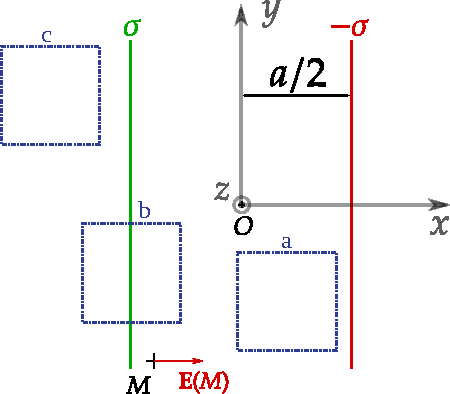
\includegraphics[scale=0.8]{condensateur}
	\caption{Condensateur plan composé d'une plaque chargée positivement avec 
	         une densité surfacique de charge $\sigma$ et une plaque chargée
	 	 négativement avec une densité surfacique de charge $-\sigma$.}%
	\label{fig:condensateur}
\end{figure}


\end{bibunit}

\begin{bibunit}
\graphicspath{{Chapitre_3/figure/}}
\chapter{Magnétostatique}
\label{chap:magnetostatique}
\section*{Objectifs}%
\label{sec:objectifs}
\begin{itemize}
	\item Connaître les équations qui contrôlent l'évolution spatiale 
	  du champ magnétostatique $\vecb$.
	\item Faire le lien entre ces équations et une carte de champ 
	  magnétique.
	\item Savoir calculer le champ magnétostatique résultant d'une 
	  distribution simple de courants.
\end{itemize}
\newpage
\section*{Introduction}
La magnétostatique étudie les champs magnétiques créés par des courants permanents.
Le plus souvent, on cherche alors à déterminer le champ magnétostatique $\vecb$
qui résulte d'une distribution de courant $\vecj$ connue. Nous nous intéressons
dans ce chapitre au champ magnétique créé par des courants circulants 
dans des conducteurs. Les milieux aimantés seront abordés plus loin dans le cours.

\section{La force de Lorentz}%
L'interaction entre deux particules immobiles a permis de définir la force de 
Coulomb dans le chapitre~\ref{chap:electrostatique}. Cette interaction 
électrostatique ne suffit plus lorsqu'il s'agit de décrire la dynamique de 
charges en mouvement. En 1895, le physicien néerlandais Hendrick Antoon Lorentz
propose alors l'ajout d'un second terme à la force coulombienne qui fait apparaître
la champ magnétostatique $\vecb$. 

\begin{defn}[Champ magnétostatique]
	Au même titre que le champ électrostatique, le champ magnétique $\vecb$
	est un champ vectoriel. Il est généré par une distribution de courant ou 
	par un aimant. Il s'exprime en tesla, noté $\tesla$ ($\kilogram \usk
	\rpsquare \second \reciprocal \ampere$ en SI). On rappelle quelques ordres de
	grandeur du champ magnétique
	
	\begin{center}
	\begin{tabular}{l|l}
		\textbf{Dispositif} 	& $\vecb (\tesla)$ \\ \hline
		Champ magnétique terrestre à la surface & $47 \times 10^{-6}$ \\
		Champ créé à $\unit{1}{\centi \meter}$ d'un fil parcouru par 
		un courant de $\unit{10}{\ampere}$
								 & $2 \times 10^{-5}$ \\
		Champ créé à $\unit{1}{\milli \meter}$ d'un aimant permanent& $0.1 - 1$ \\
		Électroaimant & $10 - 100$ \\
		Étoile à neutrons en surface & $10^{11}$\\
	\end{tabular}
	\end{center}
Le champ magnétique vérifie lui aussi le principe de superposition.
\end{defn}

\begin{defn}[Force de Lorentz]
Une particule de charge $q$ se déplaçant à la vitesse $\vecv$ dans un champ magnétique
$\vecb$, subit une force appelée force de Lorentz
\begin{equation}
	\vecf = q\vecv \wedge \vecb.
\end{equation}
Cette force est donc toujours orthogonale à la vitesse de la particule.
Contrairement à la force électrostatique, la force magnétique n'entraîne donc pas 
de variation de la vitesse de la particule, elle permet seulement de dévier sa 
trajectoire. En effet, la puissance magnétique $\mathcal{P}$ vaut
\begin{equation*}
	\mathcal{P} = \vecf \cdot \vecv = (q\vecv \wedge \vecb) \cdot \vecv = 0.
\end{equation*}
La force magnétique ne permet donc pas de mettre une particule chargée en mouvement.
\end{defn}

Comme pour la force électrostatique, le poids d'une particule chargée est bien souvent 
négligeable devant celui de la force de Lorentz. Pour illustrer cela, prenons le 
cas d'un électron de masse $m_e = \unit{9.1 \times 10^{-31}}{\kilogram}$ et de
charge $q = \unit{1.6 \times 10^{-19}}{\coulomb}$ se déplaçant à une vitesse
$v = \unit{10^5}{\meter \usk \reciprocal \second}$ dans un champ magnétique uniforme
$B = \unit{1}{\tesla}$. On trouve alors
\begin{equation*}
	\dfrac{mg}{qvB} \approx 10^{-15}.
\end{equation*}
On peut alors toujours négliger le poids d'une particule chargée
devant la force de Lorentz.

\begin{exemple}
	On s'intéresse ici au mouvement d'un électron de charge $-e$ et de 
	masse $m$ dans un 
	champ magnétique uniforme $\vecb$ (voir Fig.~\ref{fig:magneto_cyclotron}). 
	La vitesse initiale $\vecv_0$ de la particule est orthogonale au champ
	$\vecb$. La particule est donc soumise à la force de Lorentz et à son
	poids que nous négligeons ici. 
	
	Expérimentalement, on constate que la trajectoire 
	de la particule est circulaire. La force de Lorentz ne travaillant pas, 
	la norme de la vitesse reste en tout temps égale à $v_0$. Le mouvement de la 
	particule est donc uniforme et circulaire.
	
	On se place dans
	un référentiel polaire $(O, \er, \etheta)$. La position de la particule
	est donc repérée par ses coordonnées $(r, \theta)$. L'application du principe
	fondamental de la dynamique à la particule dans le référentiel du
	laboratoire supposé galiléen donne
	\begin{equation*}
		m \dot{\vecv} = q \vecv \wedge \vecb,
	\end{equation*}
	où la notation $\dot{v}$ est utilisée pour la dérivée temporelle.
	Dans un référentiel polaire et pour un mouvement circulaire uniforme, 
	$\vecv = r\dot{\theta} \etheta = v_0 \etheta$ 
	et $\dot{\vecv} = - v_0^2/r\er$. On obtient donc
	\begin{equation*}
		m \dfrac{v_0^2}{r}\er = -e v_0 \etheta \wedge \ez =e v_0 B \er \iff 
		\dot{\theta} = \dfrac{eB}{m}
	\end{equation*}
	L'électron suit donc un mouvement circulaire uniforme à la vitesse angulaire
	$eB/m$ appelée pulsation cyclotron. Dans le cyclotron de University of Michigan,
	le champ magnétique vaut $B = \unit{0.10}{\tesla}$, ce qui donne une pulsation de 
	$\unit{1.7 \times 10^{10}}{\rad \usk \reciprocal \second}$ pour un électron.

\end{exemple}
\begin{figure}[h!]
	\centering
	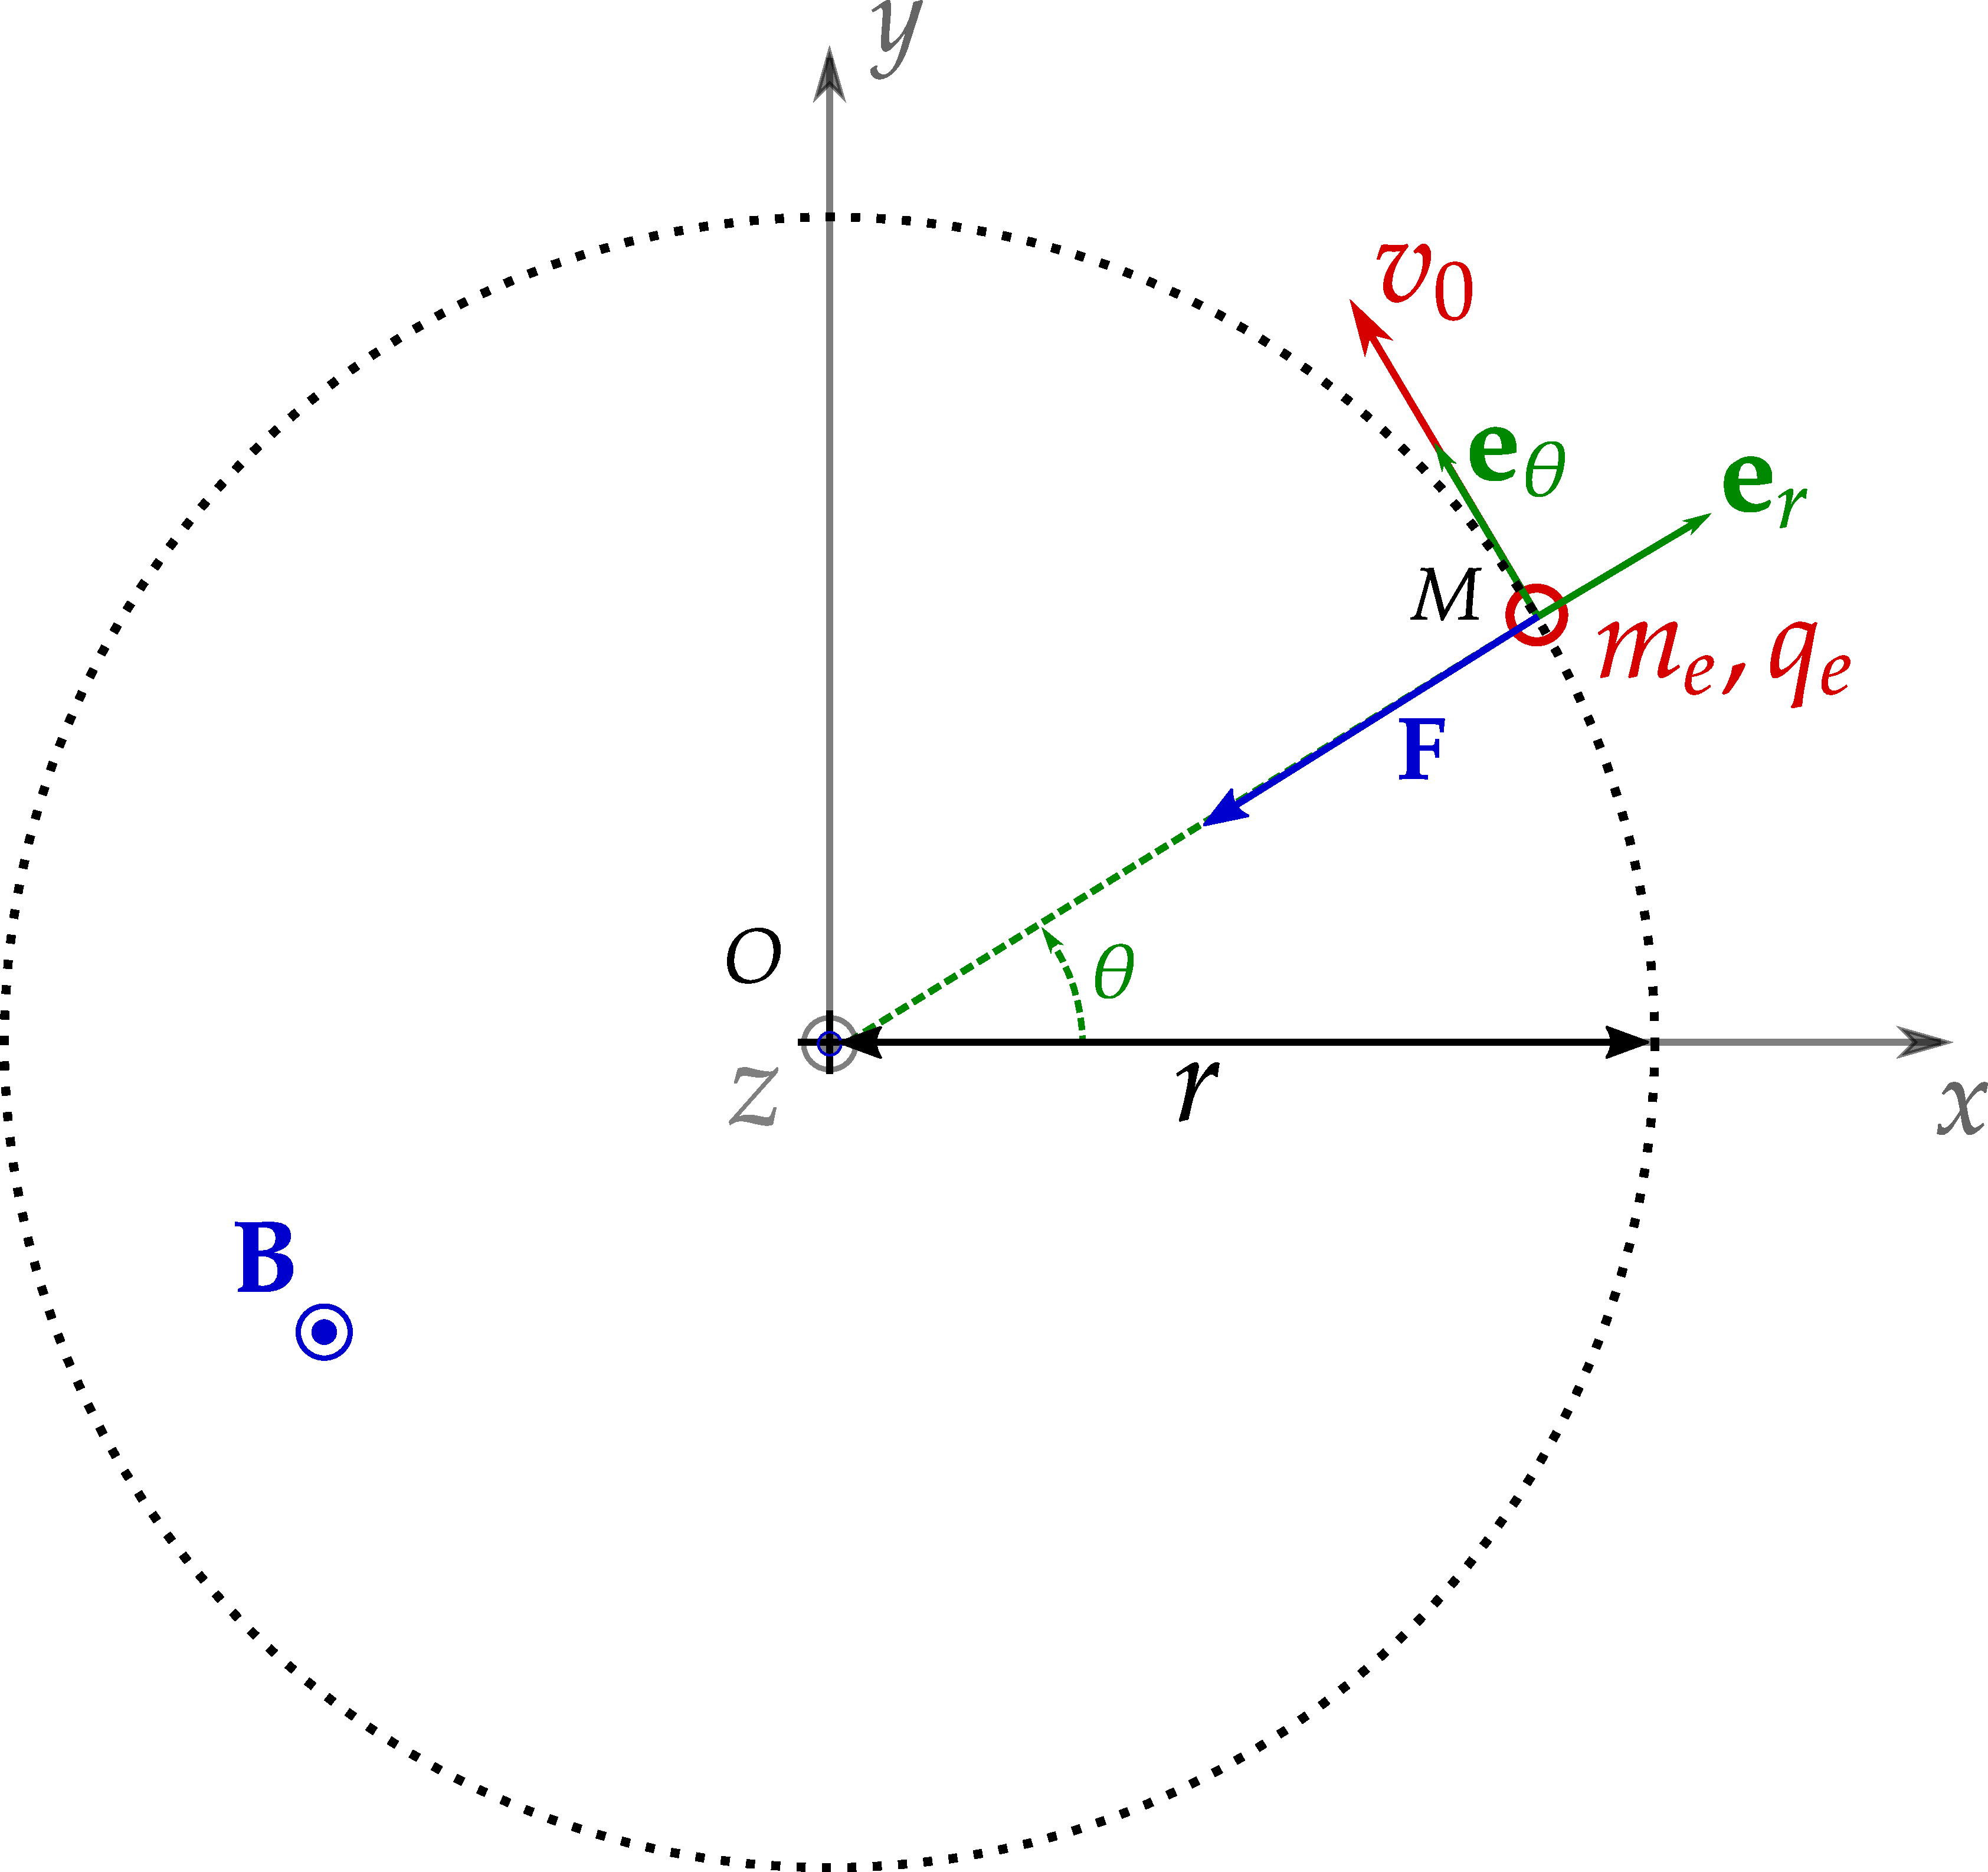
\includegraphics[scale=0.75]{cyclotron}
	\caption{Trajectoire d'un électron dans un champ magnétique uniforme.}%
	\label{fig:magneto_cyclotron}
\end{figure}

\section{La loi de Biot et Savart}
De la même manière que pour le champ électrostatique, nous
commençons par définir le champ magnétique généré par une charge ponctuelle. 
Soit une charge ponctuelle $q$ en un point $P$ de l'espace se déplaçant 
à la vitesse $\vecv$ dans le référentiel du laboratoire. Expérimentalement,
on observe que cette particule génère
en un point $M$ un champ magnétique $\vecb(M)$ tel que

\begin{equation*}
	\vecb(M) = \dfrac{\mu_0 q}{4 \pi} \vecv \wedge \dfrac{\mitbf{PM}}{||PM||^3},
\end{equation*}
où $\mu_0 = \unit{4 \pi \times 10^{-7}}{\tesla \usk \meter \usk \reciprocal 
\ampere}.$

\begin{figure}[h!]
	\centering
	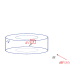
\includegraphics[]{biot_savart}
	\caption{Champ magnétique généré par un élément infinitésimal d'un conducteur
	de densité volumique de courant $\vecj$ en un point $M$ de l'espace.}%
	\label{fig:magneto_biot_savart}
\end{figure}

On considère un conducteur formant un volume $\mathcal{V}$ 
(voir Fig.~\ref{fig:magneto_biot_savart}) parcouru par des charges mobiles 
de densité volumique de charge $\rho$ se déplaçant à la vitesse $\vecv$. Un élément 
infinitésimal $\dV$ de ce circuit centré en $P$ génère en un point $M$ un champ magnétique

\begin{equation*}
	\mathrm{\textbf{d}}\mitbf{B}^P(M) = \dfrac{\mu_0 \rho(P) \dV}
	{4 \pi} \vecv(P) \wedge 
	          \dfrac{\mitbf{PM}}{||PM||^3},
\end{equation*}
où on reconnaît le vecteur densité de courant $\vecj(P) = \rho(P) \vecv(P)$. 
Le champ magnétique
$\vecb$ généré par l'ensemble du circuit en $M$ est alors obtenu en additionnant les 
contributions de chaque élément de ce dernier grâce au principe de superposition
\begin{equation*}
	\vecb(M) = \iiint_{P \in \mathcal{V}} \mathrm{\textbf{d}}\mitbf{B}^P(M)
		 = \iiint_{P \in \mathcal{V}} \dfrac{\mu_0}
		 {4 \pi} \vecj(P) \wedge 
	          \dfrac{\mitbf{PM}}{||PM||^3} \dV
\end{equation*}
On aboutit ainsi à la loi de Biot et Savart.

\begin{defn}[Loi de Biot et Savart]
	Le champ magnétostatique $\vecb(M)$ créé au point $M$ par une distribution
	volumique de courant $\vecj$ ($\ampere \usk \rpsquare \meter$) contenue
	dans un volume $\mathcal{V}$ est
	\begin{equation}
		\vecb(M) = \dfrac{\mu_0}{4 \pi} \iiint_{P \in \mathcal{V}} 
		\dfrac{\vecj(P) \wedge \mitbf{PM}}{||PM||^3} \dV,
	\end{equation}
	où $\mu_0 = \unit{4 \pi \times 10^{-7}}{\tesla \usk \meter \usk \reciprocal
	\ampere}$ est la perméabilité magnétique du vide.

\end{defn}

	Par un raisonnement similaire, on montre que pour une distribution 
	surfacique de courant $\vecj_s$ confinée sur une 
	surface $\mathcal{S}$, cette expression devient
	\begin{equation}
		\vecb(M) = \dfrac{\mu_0}{4 \pi} \iint_{P \in \mathcal{S}} 
		\dfrac{\vecj_s(P) \wedge \mitbf{PM}}{||PM||^3} \mathrm{d}S.
	\end{equation}

	Pour un circuit filiforme $\mathcal{C}$ parcouru par un courant $I$, 
	cette expression devient
	\begin{equation}
		\vecb(M) = \dfrac{\mu_0}{4 \pi} \int_{P \in \mathcal{C}} 
	\dfrac{I \dl \wedge \mitbf{PM}}{||PM||^3}.
	\end{equation}

\begin{exemple}
	On cherche à déterminer le champ magnétique généré par un fil infini $\mathcal{C}$
	parcouru
	par un courant d'intensité $I$ en un point $M$ 
	(voir Fig.~\ref{fig:magneto_spire}). On se place dans un repère cylindrique
	$(0, \er, \etheta, \ez)$. Les points $M$ et $P$ ont pour coordonnées 
	respectives $(r, \theta, 0)$ et $(0, 0, z_P)$.

	Le champ magnétique $\mathrm{\textbf{d}}\vecb^P(M)$ généré par un élément
	$\dl_P$ du fil centré en $P$ s'écrit
	\begin{equation*}
	\mathrm{\textbf{d}}\vecb^P(M) = \dfrac{\mu_0}{4 \pi} 
	              \dfrac{I \dl_P \wedge \mitbf{PM}}{||PM||^3},
	\end{equation*}
	où $\mitbf{PM} = \mitbf{PO} + \mitbf{OM} = - z_P\ez + r\er$. Dans un repère
	cylindrique, un élément infinitésimal $\dl_P$ du fil s'écrit
	$\dl_P = \dz_P \ez$. On a alors
	\begin{equation*}
		\dfrac{\dl_P \wedge \mitbf{PM}}{||PM||^3} = 
		\dfrac{r\dz_P}{||PM||^3}\etheta. 	
	\end{equation*}
	En remarquant que $||PM|| = r/\cos\alpha$, l'expression précédente devient alors
	\begin{equation*}
		\dfrac{r\dz_P}{||PM||^3}\etheta = \dfrac{\cos^3\alpha \dz_P}
		{r^2} \etheta
	\end{equation*}
	De même, on remarque que $z_p = r \tan\alpha$.
	Par différentiation, on obtient donc
	\begin{equation*}
		\dz_P = \mathrm{d}\left[r\tan\alpha\right] = 
		\dfrac{r \mathrm{d}\alpha}{\cos^2\alpha}.
	\end{equation*}
	Finalement,
	\begin{equation*}
		\mathrm{\textbf{d}}\vecb^P(M) = \dfrac{\mu_0 I \cos\alpha}
		{4 \pi r} \mathrm{d}\alpha \etheta.
	\end{equation*}
	Le champ $\vecb(M)$ généré au point $M$ par le fil s'obtient alors
	en utilisant le principe de superposition, ce qui revient à intégrer les champs 
	magnétiques infinitésimaux sur l'ensemble du fil. Pour parcourir l'ensemble du
	fil, $\alpha$ doit varier entre $-\pi/2$ et $\pi/2$. On a alors
	\begin{equation*}
		\boxed{\vecb(M) = \dfrac{\mu_0 I}{4\pi r}
			\times \displaystyle{\int_{-\pi/2}^{\pi/2} 
			\cos\alpha\mathrm{d}\alpha \etheta} =
	\dfrac{\mu_0 I}{2\pi r}\etheta.}
	\end{equation*}
	On obtient un champ magnétique porté par $\etheta$ et donc la norme ne dépend
	que de $r$. Les lignes de ce champ sont des cercles concentriques centrés
	sur le fil. $\vecb$ "tourne" autour du fil.
\end{exemple}
\begin{figure}[h!]
	\centering
	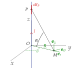
\includegraphics[scale=0.7]{fil}
	\caption{Champ magnétique créé en un point $M$ par un fil parcouru par
	un courant d'intensité $I$.}%
	\label{fig:magneto_spire}
\end{figure}

\begin{defn}[Calcul du champ magnétique par la loi de Biot et Savart]
	Comme nous l'avons vu dans l'exemple précédent, la loi de Biot et Savart
	peut s'avérer utile lorsqu'il s'agit de calculer le champ magnétique 
	$\vecb$ généré par une distribution de courant. Voici en résumé la démarche à suivre
	\begin{enumerate}
		\item Réaliser un schéma du système et choisir un repère adapaté.
		\item Exprimer le petit volume $\dV$, de surface $\mathrm{d}S$
		  ou de longueur $\dl$ dans ce système de coordonnées.
	  \item En multipliant cet élément par le courant ($\vecj$, $\vecj_s$ ou
	    $I$), on obtient le petit élément de courant associé.
	  \item Exprimer le vecteur $\mitbf{PM}$ dans le système de coordonnées
	    choisi.
    	\item En multipliant par $\dfrac{\mu_0}{4 \pi}$ et en faisant le produit 
	  vectoriel par $\dfrac{\mitbf{PM}}{||PM||^3}$, on fabrique le champ
	  élémentaire $\mathrm{\textbf{d}}\vecb^P(M)$ généré en $M$.
	\item Pour calculer $\vecb(M)$, il suffit alors d'intégrer sur la distribution
	  de courant.
	\end{enumerate}
\end{defn}
\section{Équation de la magnétostatique}
On considère un fil parcouru par un courant $I$ dans un
repère cylindrique $(O, \er, \etheta, \ez)$ (voir Fig.~\ref{fig:magneto_spire}). 
Comme vu ci-dessus, le champ
magnétique créé par ce fil en un point $M$ situé à une distance $r$ du fil
est donné par
\begin{equation*}
	\vecb(M) = \dfrac{\mu_0 I}{2 \pi r}\etheta.
\end{equation*}
Comme pour le champ électrostatique, nous allons nous servir de cet exemple simple 
pour retrouver certaines propriétés du champ magnétostatique.

\subsection{Le théorème d'Ampère}
Le théorème d'Ampère est l'équivalent pour le champ magnétostatique $\vecb$
du théorème de Gauss. Il va nous permettre de calculer facilement le champ
magnétostatique généré par une distribution de courants simple.

Les lignes du champ $\vecb$ créé par le fil sont des cercles dont l'axe est le
fil. Nous cherchons donc dans un premier temps à calculer la circulation de $\vecb$ 
sur la ligne de champ $\mathcal{C}$ de rayon $r$ passant par $M$. 
On a bien pris soin au préalable
d'orienter cette dernière. Dans un repère cylindrique, un petit élément $\dl$ de ce 
contour fermé s'écrit $\dl = r \dtheta \etheta$. La circulation de $\vecb$ sur
ce contour s'écrit donc
\begin{equation*}
	\boxed{\displaystyle{\oint_\mathcal{C} \vecb \cdot \dl = 
		\oint_0^{2 \pi} \dfrac{\mu_0 I}{2 \pi r} r\dtheta
	= \mu_0 I.}}
\end{equation*}
On constate que la circulation du champ $\vecb$ le long du circuit $\mathcal{C}$
ne dépend que du courant $I$ que ce dernier enlace. Cette propriété que nous venons
de montrer pour un fil est en fait une propriété générale du champ magnétostatique.

\begin{defn}[Théorème d'Ampère]
	La circulation du champ magnétostatique $\vecb$ le long d'un circuit fermé
	$\mathcal{C}$ est égale au courant \textbf{algébrique} $I_\mathrm{int}$ 
	enlacé par ce dernier multiplié
	par $\mu_0$
	\begin{equation}
		\oint_\mathcal{C} \vecb \cdot \dl = \mu_0 I_\mathrm{int}.
	\end{equation}
	Le contour sur lequel est réalisée l'intégrale est appelé contour d'Ampère.
	Le courant enlacé $I_\mathrm{int}$ est le courant qui traverse une surface 
	orientée
	qui s'appuie sur le contour d'Ampère. L'orientation de la surface 
	se déduit de celle du contour
	grâce à la règle de la main droite ou du tire-bouchon.
\end{defn}

\begin{exemple}
	\begin{minipage}{0.6\linewidth}
	Soit deux fils électriques parcourus par des courants $I_1$ et $I_2$.
	Avec les orientations choisies, le théorème d'Ampère appliqué au 
	contour $\mathcal{C}$ s'écrit
	\begin{equation*}
		\oint_\mathcal{C} \vecb \cdot \dl = \mu_0(I_1 - I_2).
	\end{equation*}
	\end{minipage}
	\hfill
	\begin{minipage}{0.35\linewidth}
		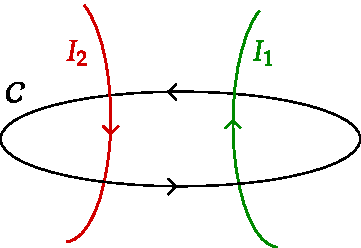
\includegraphics[width=0.8\linewidth]{ampere_ex}
	\end{minipage}

\end{exemple}

Le théorème d'Ampère peut-être traduit sous une forme locale:
appelée \textbf{équation de Maxwell-Ampère}, qui relie alors le champ magnétostatique
au vecteur densité de courant.

\begin{defn}[Équation de Maxwell-Ampère]
	L'équation de Maxwell-Ampère relie le champ magnétostatique $\vecb$
	au vecteur densité de courant $\vecj$
	\begin{equation}
		\rot \vecb = \mu_0 \vecj.
		\label{eq:magneto_ma}
	\end{equation}
	Cette équation est une relation $\textbf{locale}$, elle permet de relier 
	les dérivées spatiales du champ $\vecb$ en un point de l'espace au vecteur
	$\vecj$ en ce même point.
\end{defn}

\subsection{Flux du champ magnétostatique $\vecb$}
On cherche maintenant à calculer la divergence du champ $\vecb$. En coordonnées 
cylindriques, cela donne
\begin{equation*}
	\div \vecb = \dfrac{1}{r}\left(\dd{r B_r}{r} + \dd{B_\theta}{\theta} \right)
	+ \dd{B_z}{z},
\end{equation*}
où $B_r$, $B_\theta$ et $B_z$ sont les composantes de $\vecb$. 
Dans le cas du fil infini, $B_\theta$ est la seule composante non nulle de $\vecb$ 
et elle ne dépend pas
de $\theta$. On a donc
\begin{equation*}
	\div \vecb = 0.
\end{equation*}
Ce résultat se généralise à un champ magnétostatique $\vecb$ quelconque sous
la forme de l'équation de Maxwell-Thomson.

\begin{defn}[Équation de Maxwell-Thomson]
	Un champ magnétique $\vecb$ vérifie toujours
	\begin{equation*}
		\div \vecb = 0.
	\end{equation*}
	Cette relation locale est vérifiée en tout point de l'espace.
\end{defn}

\begin{rem}
La divergence de $\vecb$ étant nulle, l'analyse vectorielle affirme
qu'il est possible dans ce cas de définir un champ vectoriel $\veca$,
défini à un gradient près, tel que $\rot \veca = \vecb$,
appelé le potentiel vecteur.
\end{rem}

Comme l'équation de Maxwell-Ampère, cette équation peut se mettre sous une forme
intégrale, en exprimant le flux du champ magnétique à travers une surface fermée
$\mathcal{S}$.

\begin{defn}[Flux du champ magnétostatique]
	Le flux du champ magnétique $\vecb$ à travers une surface fermée 
	$\mathcal{S}$ est nul
	\begin{equation*}
		\oiint_\mathcal{S} \vecb \cdot \ds = 0.
	\end{equation*}
	On dit que le champ $\vecb$ est à flux conservatif.
\end{defn}

	\begin{minipage}{0.6\linewidth}
	On peut appliquer ce résultat à une surface $\mathcal{S}$ particulière
	constituée d'une portion de tube de champ de section d'entrée $\mathcal{S}_e$,
	de section de sortie $\mathcal{S}_s$ et de section latérale $
	\mathcal{S}_l$. 	
	\end{minipage}
	\hfill
	\begin{minipage}{0.3\linewidth}
	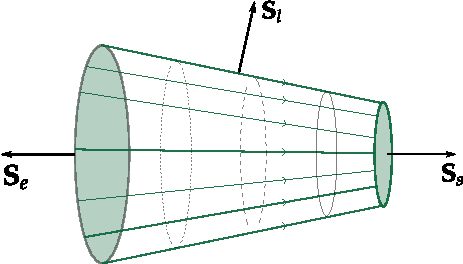
\includegraphics[scale=0.7]{tube}
	\end{minipage}
	\vspace{0.5cm}

\begin{defn}[Tube de champ]
	L'ensemble des lignes de champ s'appuyant sur un contour fermé forme un 
	tube de champ.
\end{defn}
	
	D'après le théorème d'Ampère la flux de $\vecb$ à
	travers cette surface est nul.
	Par définition du tube de champ, l'intégrale sur la surface 
	latérale est nulle. Il reste donc 
	\begin{equation*}
		\iint_\mathcal{S_e} \vecb \cdot \ds_e =
		- \iint_\mathcal{S_s} \vecb \cdot \ds_s 
		\iff
		\displaystyle{\left\lvert\iint_\mathcal{S_e} \vecb \cdot \ds_e\right\rvert =
		\left\lvert\iint_\mathcal{S_s} \vecb \cdot \ds_s\right\rvert}.
	\end{equation*}
	Le flux entrant dans la surface est égal au flux sortant de cette dernière.
	De plus, la surface de sortie étant de taille plus importante que 
	la surface d'entrée, on en conclut que le champ est plus intense
	à l'entrée du tube qu'à la sortie. Le champ $\vecb$ étant à flux
	conservatif, un resserrement des lignes de champs traduit une augmentation
	de l'intensité de ce dernier.

\begin{defn}[Flux conservatif et lignes de champ]
	Le champ magnétique étant à flux conservatif, ses lignes de champs
	se resserrent dans les zones de forte intensité. Inversement, ces dernières
	s'éloignent lorsqu'il devient plus faible
\end{defn}

\section{Étude des lignes de champ de \vecb}
Nous nous intéressons dans cette partie aux propriétés spatiales du champ $\vecb$.
Nous allons voir comment les \textbf{lignes de champ} nous renseignent sur sa répartition 
dans l'espace.

Nous nous intéressons au champ magnétique produit par un solénoïde 
(voir Fig.~\ref{fig:magneto_solenoide}).
Les lignes de champ nous permettent de retrouver quelques propriétés du champ 
magnétostatique énoncées précédemment.

\begin{figure}[htpb]
	\centering
	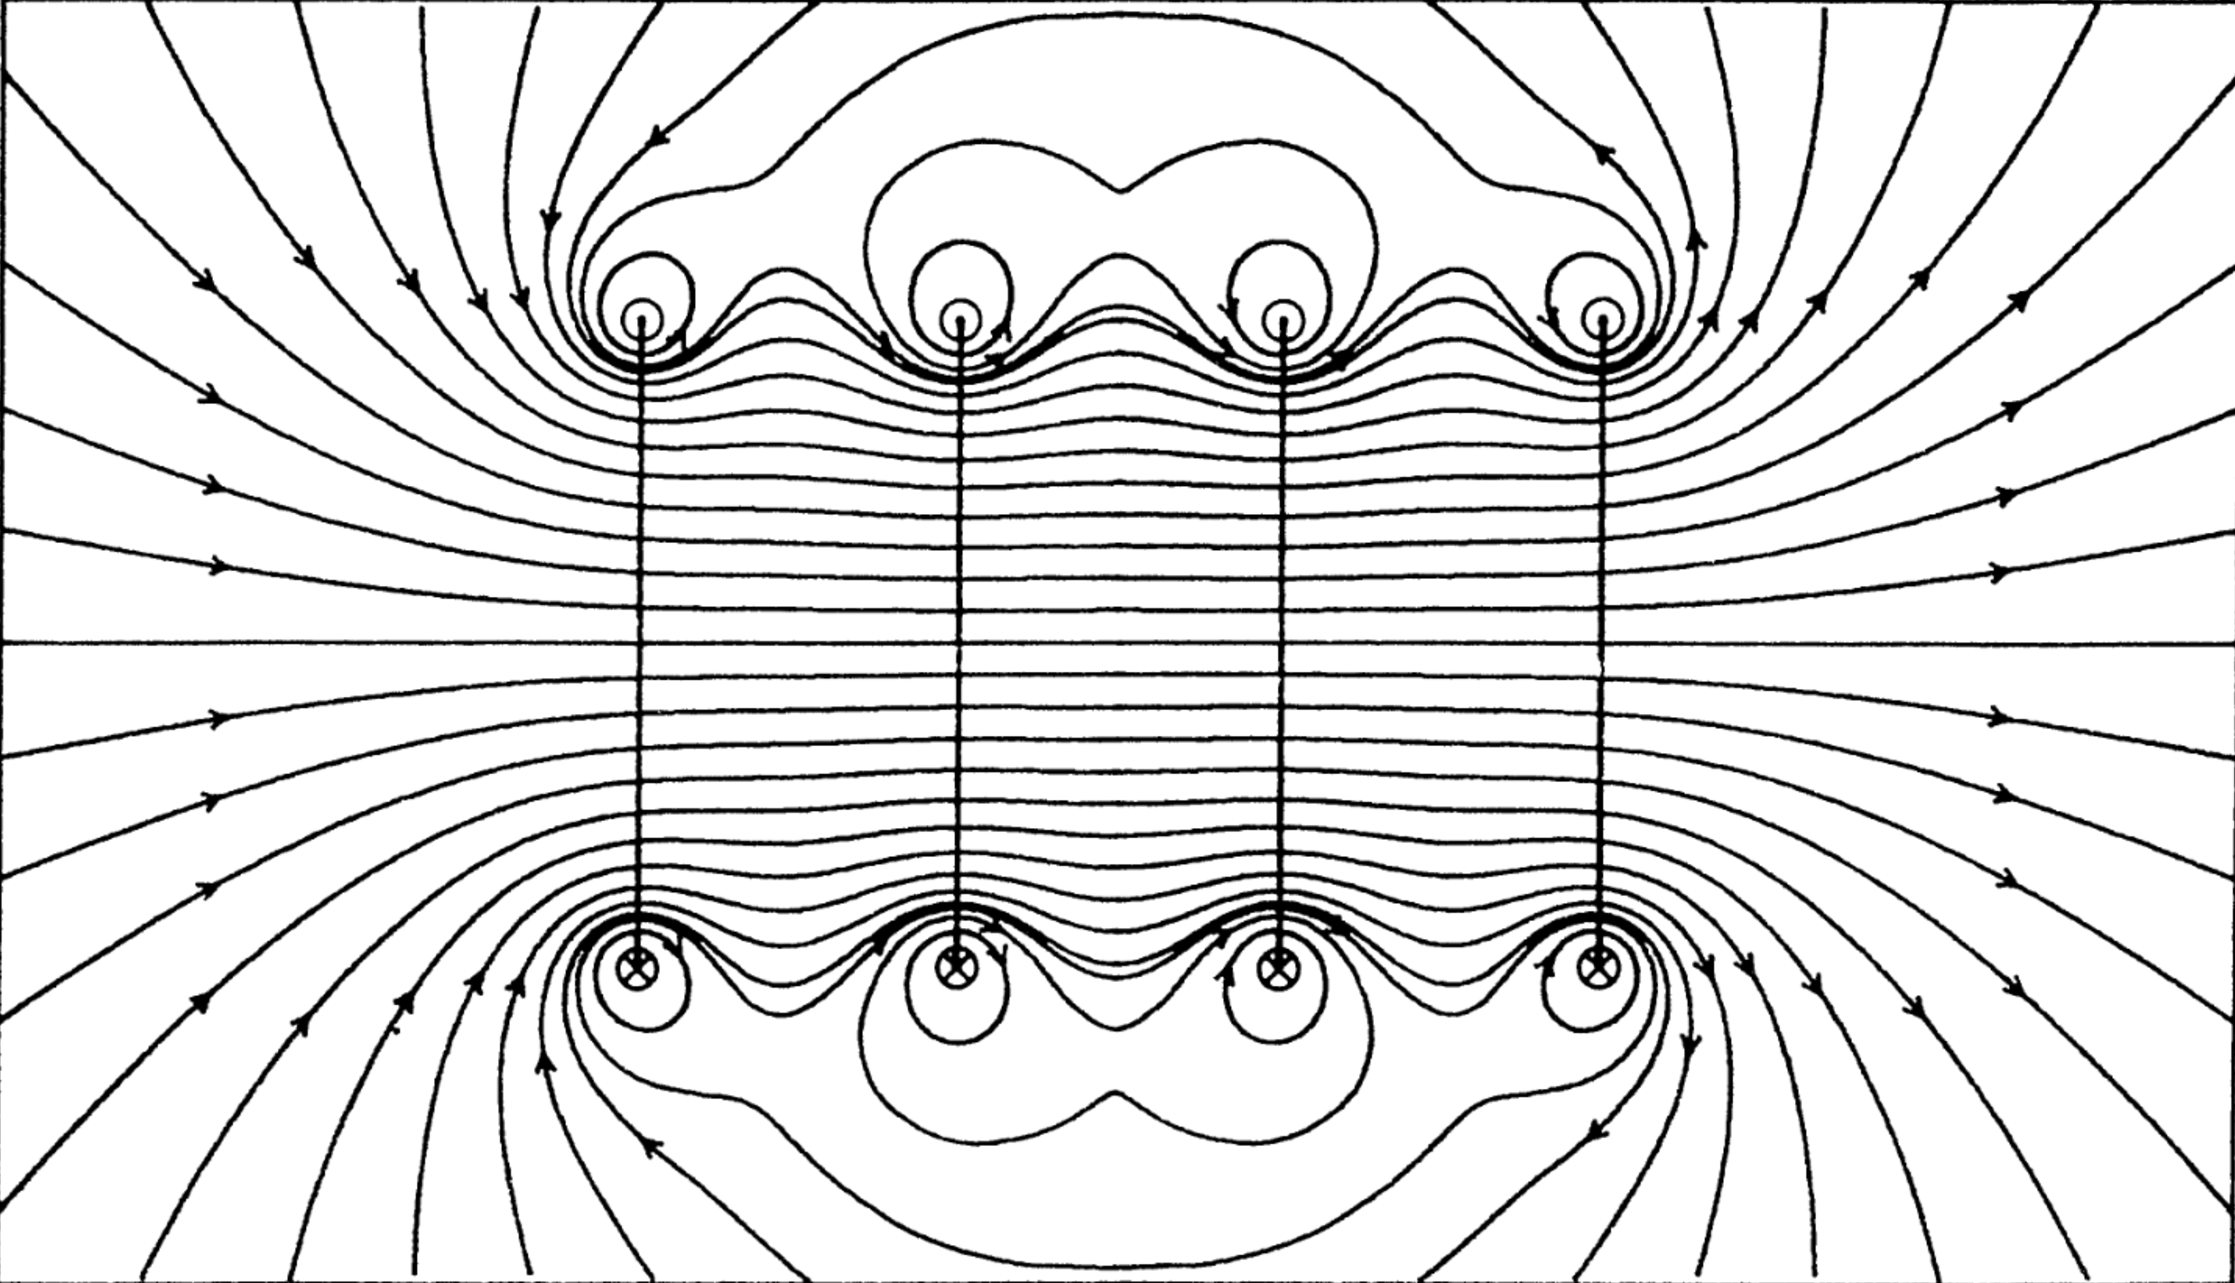
\includegraphics[width=0.7\linewidth]{solenoide}
	\caption{Lignes du champ magnétique généré par un solénoïde constitué de
		4 bobines parcourues dans le même sens par la même intensité.
		Cette figure est extraite de \cite{Gie1985}}%
	\label{fig:magneto_solenoide}
\end{figure}

\begin{enumerate}
	\item On remarque tout d'abord que les lignes de champ 
	  sont des contours fermés qui entourent les fils parcourus par un courant.
	  Cette première observation est une conséquence directe de l'équation
	  de Maxwell-Ampère. L'orientation de ces lignes de champ s'obtient
	  d'ailleurs en considérant le sens du courant dans les fils et en utilisant
	  la règle de la main droite.
      \item La divergence nulle de $\vecb$ est aussi visible sur cette carte de 
	champ. En effet, on constate que les lignes de champ ne convergent/divergent
	pas en un point de l'espace, contrairement au champ électrostatique.
      \item Dans le cas du champ magnétique, le resserrement des lignes de champ
	traduit une augmentation de la norme de ce dernier. On conclut que le champ
	est plus intense à l'intérieur du solénoïde qu'à l'extérieur. De plus, les
	lignes de champ étant parallèles à l'intérieur du solénoïde, on conclut que
	le champ est uniforme.
      \item Grâce aux lignes de champ, on retrouve rapidement les plans de 
	  symétrie et d'antisymétrie du champ magnétique. Le plan médiateur 
	  du solénoïde est par exemple un plan de symétrie du champ magnétique. 
          L'analyse de ces symétries sera utile pour calculer le champ
          magnétique résultant d'une distribution de courant.
\end{enumerate}

\section{Calcul du champ magnétostatique}
\label{sec:calcul_e}
Nous allons voir dans cette partie comment nous pouvons utiliser le théorème d'Ampère
pour calculer le champ magnétostatique $\vecb$ créé 
par une distribution de courants simple. Nous nous intéressons ici à une bobine
torique constituée d'un fil régulièrement bobiné autour d'un tore de section
carré (voir Fig.~\ref{fig:magneto_tore}). Cette bobine est caractérisée par le nombre $N$
total de spires bobinés, son rayon intérieur $R$ 
et sa hauteur $h$. La bobine est parcourue par un courant $I$.

On cherche à déterminer 
l'expression du champ électrique $\vecb$ en un point $M$ de l'espace. Pour ce faire, 
il suffit de suivre le mode d'emploi suivant
\begin{enumerate}
	\item Faire un schéma du système ! C'est absolument indispensable
	  (voir Fig.~\ref{fig:magneto_tore})
	\item Choisir un repère adapté au problème
	\item Étudier les invariances de cette distribution
	\item Étudier les symétries de la distribution de courants à l'origine 
	  du champ magnétostatique
	\item Choisir un contour d'Ampère et appliquer le théorème d'Ampère.
\end{enumerate}

Au vu de la géométrie du système, nous choisissons ici d'utiliser 
un repère cylindrique $(O, \er, \etheta, \ez)$.
Le point $M$ est donc repéré par ses coordonnées $(r, \theta, z)$. Le champ
magnétostatique en $M$ s'écrit de manière générale

\begin{equation}
	\vecb(M) = B_r(M)\er + B_\theta(M)\etheta + B_\varphi(M)\ephi.
	\label{eq:tore}
\end{equation}
Le champ magnétostatique est un vecteur à trois composantes et chaque composante
dépend des coordonnées de $M$. Pour simplifier cette expression, il est intéressant
de considérer les invariances et symétries de la distribution de courant qui génère
le champ $\vecb$.

\begin{figure}
	\centering
	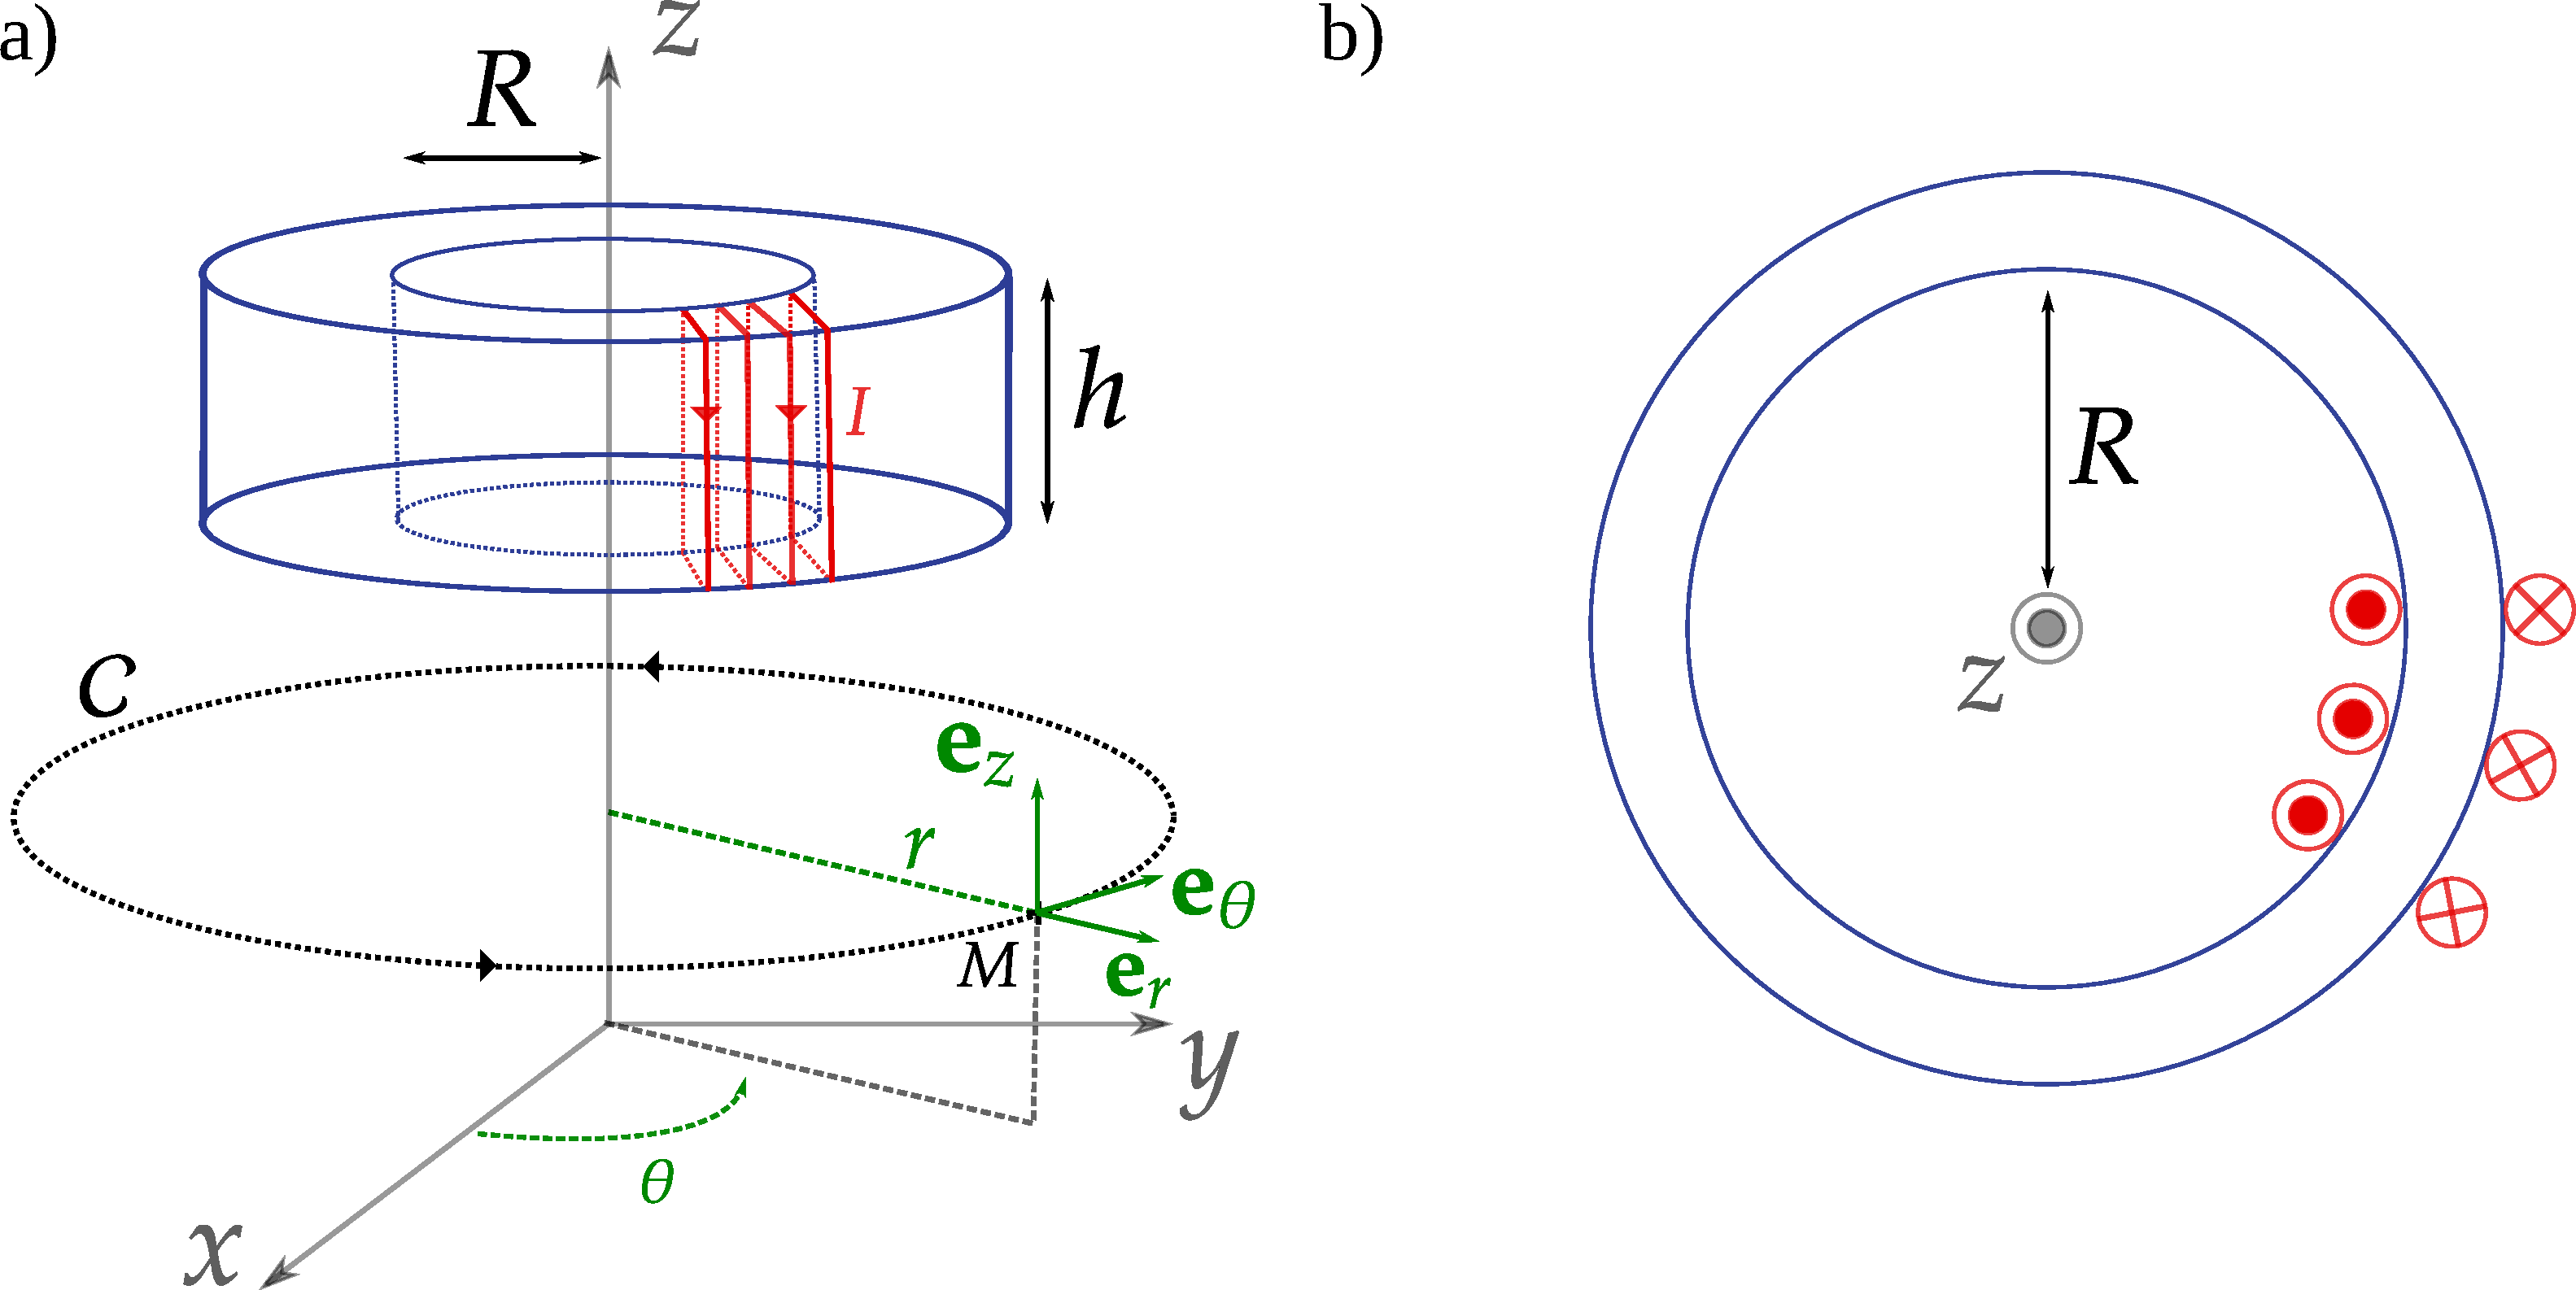
\includegraphics[scale=1]{tore}
	\caption{Bobine torique à gauche et coupe perpendiculaire à $(Oz)$
	de cette bobine à droite.}%
	\label{fig:magneto_tore}
\end{figure}

\subsection{Invariance de la distribution de courants}
On cherche ici à savoir si la distribution de courant est modifiée sous l'effet
d'une translation ou d'une rotation de l'espace. En d'autres termes, on regarde
de quelles variables elle dépend. Étant donné que les spires sont uniformément
répartie sur le tore, on observe que

\begin{itemize}
	\item  si je tourne le tore d'un angle $\Delta \theta$ dans la
	  direction $\etheta$, le problème
	  ne change pas. La distribution de courant est donc invariante 
	  par rotation selon l'angle $\theta$. $\vecb$ \textbf{ne dépend pas de
	  $\mitbf{\theta}$}.
\end{itemize}

Finalement, l'expression~\ref{eq:tore} du champ magnétique se simplifie donc en 

\begin{equation*}
	\boxed{\vecb(M) = B_r(r,z)\er + B_\theta(r,z)\etheta + B_z(r,z)\ez.}
\end{equation*}
\subsection{Symétries de la distribution de courants}

Si on applique ce principe au champ magnétique créé par une distribution 
de courants, cela revient à dire que les symétries de la distributions de 
courants doivent se retrouver dans les symétries du champ magnétique. On en 
déduit les règles suivantes

\begin{defn}[Symétries de $\vecb$ et de la distribution de courant]
\begin{itemize}
  \item si $(\Pi)$ est un plan d'antisymétrie de la distribution de courant et que 
    $M$ appartient à $(\Pi)$, alors obligatoirement $\vecb(M)$ doit 
    appartenir à $(\Pi)$,
  \item si $(\Pi)$ est un plan de symétrie de la distribution de courant 
    et que $M$ appartient à $(\Pi)$, alors obligatoirement $\vecb(M)$ doit 
    être orthogonal à $(\Pi)$.
\end{itemize}
\end{defn}

\begin{rem}
	Le champ magnétostatique $\vecb$ appartient aux plans d'\textbf{antisymétrie}
	de la distribution de courant et non aux plans de symétrie comme
	c'est le cas pour le champ électrostatique. Le vecteur $\vecb$ est 
	qualifié de vecteur axial.
\end{rem}

Pour appliquer ces règles à notre exemple, on détermine les plans de symétrie 
et d'antisymétrie de la distribution de courants auquels 
le point $M$ appartient

\begin{itemize}
	\item le plan $(M, \er, \ez)$ est un plan de symétrie de la distribution
	  de courant. $\vecb(M)$ \textbf{doit être orthogonal à ce plan}.
\end{itemize}

$\vecb(M)$ doit être orthogonal au plan $(M, \er, \ez)$, 
il doit donc être colinéaire à $\etheta$

\begin{framed}
\begin{equation*}
	\vecb(M) = B_\theta(r, z) \etheta.
\end{equation*}
\end{framed}

Nous n'avons imposé aucune condition sur la position de $M$, cette relation est
donc vraie pour tout point $M$ de l'espace. Maintenant que l'expression du 
champ magnétique a été simplifiée au maximum, on cherche à appliquer le théorème
d'Ampère.

\subsection{Application du théorème d'Ampère}
La distribution de courant présente une symétrie de révolution. On choisit comme contour 
d'Ampère un cercle $\mathcal{C}$ de rayon $r$, de centre $O$ et orienté
dans le sens de $\etheta$ qui passe par $M$ 
(voir Fig~\ref{fig:magneto_tore}) et on applique le théorème d'Ampère à ce dernier

\begin{equation*}
	\oint_\mathcal{S} \vecb(M) \cdot \dl = \mu_0 I_\mathrm{int},
	\label{eq:cavite_gauss}
\end{equation*}
où $I_\mathrm{int}$ est la courant enlacé par $\mathcal{C}$. On commence
par déterminer l'expression du membre de gauche. Dans un repère cylindrique,

\begin{equation*}
	\dl = r \dtheta \etheta.
\end{equation*}
On obtient alors
\begin{equation*}
	\oint_\mathcal{C} \vecb(M) \cdot \dl = 
	\oint_\mathcal{C} B(r,z) \etheta \cdot r \dtheta \etheta
	= B(r, z) r \int_0^{2 \pi} \dtheta
	= 2 \pi r B(r,z).
\end{equation*}
On s'intéresse maintenant au terme de droite de l'équation.
Deux cas de figure se présentent:
\begin{itemize}
	\item $M$ est situé dans le tore: le courant enlancé par $\mathcal{C}$ est alors
	  $I_\mathrm{int} = NI$.
       \item $M$ est situé à l'extérieur du tore: le courant enlacé par 
	       $\mathcal{C}$ est donc nul. Soit parce que le contour n'enlace 
	       aucun courant, soit parce qu'il enlace autant de courants positifs
	       que de courants négatifs.
\end{itemize}
Finalement,
\begin{framed}
\begin{itemize}
	\item si $M$ se trouve à l'intérieur du tore, 
	  $\vecb(M) = \dfrac{\mu_0 N I}{2 \pi r} \etheta$.
	\vspace{1em}
\item si $M$ est en dehors du tore, $\vecb(M) = \mitbf{0}$. 
\end{itemize}
\end{framed}
%\nocite{*}
%\putbib[magnetostatique]

%\newpage

%\chapter{Magnétostatique}
\label{chap:magnetostatique}
\section*{Objectifs}%
\label{sec:objectifs}
\begin{itemize}
	\item Connaître les équations qui contrôlent l'évolution spatiale 
	  du champ magnétostatique $\vecb$.
	\item Faire le lien entre ces équations et une carte de champ 
	  magnétique.
	\item Savoir calculer le champ magnétostatique résultant d'une 
	  distribution simple de courants.
\end{itemize}
\newpage
\section*{Introduction}
La magnétostatique étudie les champs magnétiques créés par des courants permanents.
Le plus souvent, on cherche alors à déterminer le champ magnétostatique $\vecb$
qui résulte d'une distribution de courant $\vecj$ connue. Nous nous intéressons
dans ce chapitre au champ magnétique créé par des courants circulants 
dans des conducteurs. Les milieux aimantés seront abordés plus loin dans le cours.

\section{La force de Lorentz}%
L'interaction entre deux particules immobiles a permis de définir la force de 
Coulomb dans le chapitre~\ref{chap:electrostatique}. Cette interaction 
électrostatique ne suffit plus lorsqu'il s'agit de décrire la dynamique de 
charges en mouvement. En 1895, le physicien néerlandais Hendrick Antoon Lorentz
propose alors l'ajout d'un second terme à la force coulombienne qui fait apparaître
la champ magnétostatique $\vecb$. 

\begin{defn}[Champ magnétostatique]
	Au même titre que le champ électrostatique, le champ magnétique $\vecb$
	est un champ vectoriel. Il est généré par une distribution de courant ou 
	par un aimant. Il s'exprime en tesla, noté $\tesla$ ($\kilogram \usk
	\rpsquare \second \reciprocal \ampere$ en SI). On rappelle quelques ordres de
	grandeur du champ magnétique
	
	\begin{center}
	\begin{tabular}{l|l}
		\textbf{Dispositif} 	& $\vecb (\tesla)$ \\ \hline
		Champ magnétique terrestre à la surface & $47 \times 10^{-6}$ \\
		Champ créé à $\unit{1}{\centi \meter}$ d'un fil parcouru par 
		un courant de $\unit{10}{\ampere}$
								 & $2 \times 10^{-5}$ \\
		Champ créé à $\unit{1}{\milli \meter}$ d'un aimant permanent& $0.1 - 1$ \\
		Électroaimant & $10 - 100$ \\
		Étoile à neutrons en surface & $10^{11}$\\
	\end{tabular}
	\end{center}
Le champ magnétique vérifie lui aussi le principe de superposition.
\end{defn}

\begin{defn}[Force de Lorentz]
Une particule de charge $q$ se déplaçant à la vitesse $\vecv$ dans un champ magnétique
$\vecb$, subit une force appelée force de Lorentz
\begin{equation}
	\vecf = q\vecv \wedge \vecb.
\end{equation}
Cette force est donc toujours orthogonale à la vitesse de la particule.
Contrairement à la force électrostatique, la force magnétique n'entraîne donc pas 
de variation de la vitesse de la particule, elle permet seulement de dévier sa 
trajectoire. En effet, la puissance magnétique $\mathcal{P}$ vaut
\begin{equation*}
	\mathcal{P} = \vecf \cdot \vecv = (q\vecv \wedge \vecb) \cdot \vecv = 0.
\end{equation*}
La force magnétique ne permet donc pas de mettre une particule chargée en mouvement.
\end{defn}

Comme pour la force électrostatique, le poids d'une particule chargée est bien souvent 
négligeable devant celui de la force de Lorentz. Pour illustrer cela, prenons le 
cas d'un électron de masse $m_e = \unit{9.1 \times 10^{-31}}{\kilogram}$ et de
charge $q = \unit{1.6 \times 10^{-19}}{\coulomb}$ se déplaçant à une vitesse
$v = \unit{10^5}{\meter \usk \reciprocal \second}$ dans un champ magnétique uniforme
$B = \unit{1}{\tesla}$. On trouve alors
\begin{equation*}
	\dfrac{mg}{qvB} \approx 10^{-15}.
\end{equation*}
On peut alors toujours négliger le poids d'une particule chargée
devant la force de Lorentz.

\begin{exemple}
	On s'intéresse ici au mouvement d'un électron de charge $-e$ et de 
	masse $m$ dans un 
	champ magnétique uniforme $\vecb$ (voir Fig.~\ref{fig:magneto_cyclotron}). 
	La vitesse initiale $\vecv_0$ de la particule est orthogonale au champ
	$\vecb$. La particule est donc soumise à la force de Lorentz et à son
	poids que nous négligeons ici. 
	
	Expérimentalement, on constate que la trajectoire 
	de la particule est circulaire. La force de Lorentz ne travaillant pas, 
	la norme de la vitesse reste en tout temps égale à $v_0$. Le mouvement de la 
	particule est donc uniforme et circulaire.
	
	On se place dans
	un référentiel polaire $(O, \er, \etheta)$. La position de la particule
	est donc repérée par ses coordonnées $(r, \theta)$. L'application du principe
	fondamental de la dynamique à la particule dans le référentiel du
	laboratoire supposé galiléen donne
	\begin{equation*}
		m \dot{\vecv} = q \vecv \wedge \vecb,
	\end{equation*}
	où la notation $\dot{v}$ est utilisée pour la dérivée temporelle.
	Dans un référentiel polaire et pour un mouvement circulaire uniforme, 
	$\vecv = r\dot{\theta} \etheta = v_0 \etheta$ 
	et $\dot{\vecv} = - v_0^2/r\er$. On obtient donc
	\begin{equation*}
		m \dfrac{v_0^2}{r}\er = -e v_0 \etheta \wedge \ez =e v_0 B \er \iff 
		\dot{\theta} = \dfrac{eB}{m}
	\end{equation*}
	L'électron suit donc un mouvement circulaire uniforme à la vitesse angulaire
	$eB/m$ appelée pulsation cyclotron. Dans le cyclotron de University of Michigan,
	le champ magnétique vaut $B = \unit{0.10}{\tesla}$, ce qui donne une pulsation de 
	$\unit{1.7 \times 10^{10}}{\rad \usk \reciprocal \second}$ pour un électron.

\end{exemple}
\begin{figure}[h!]
	\centering
	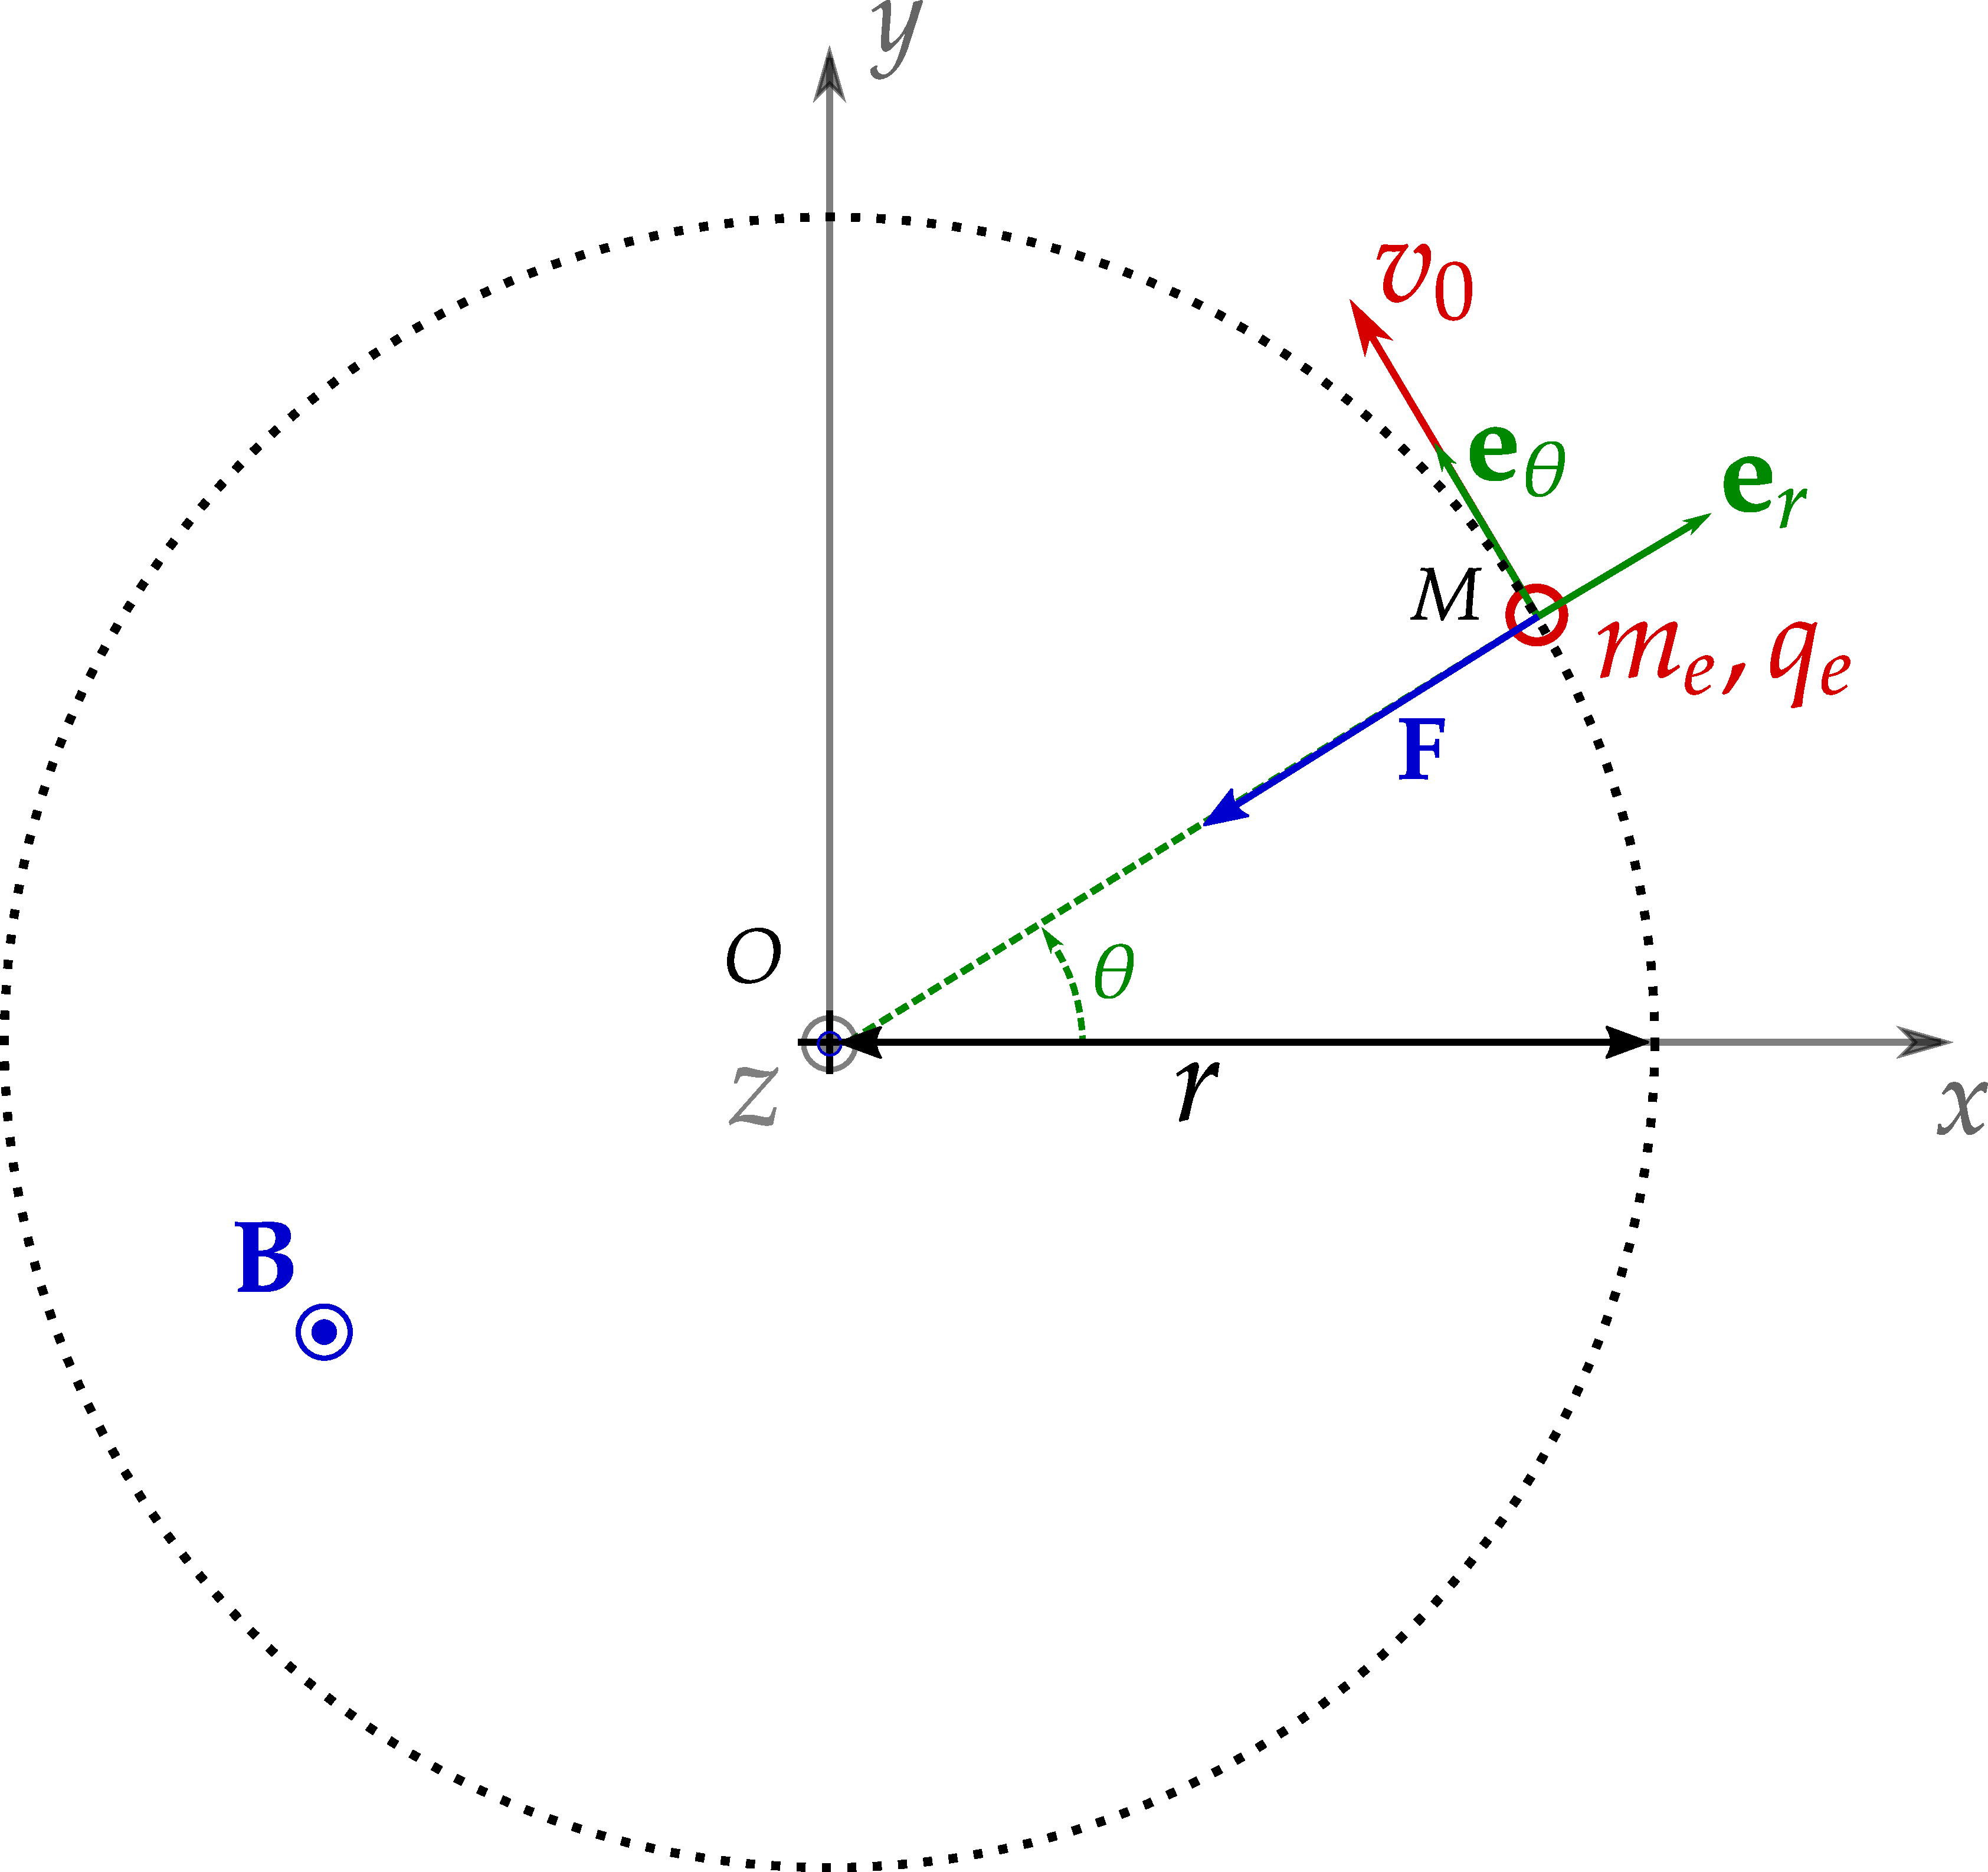
\includegraphics[scale=0.75]{cyclotron}
	\caption{Trajectoire d'un électron dans un champ magnétique uniforme.}%
	\label{fig:magneto_cyclotron}
\end{figure}

\section{La loi de Biot et Savart}
De la même manière que pour le champ électrostatique, nous
commençons par définir le champ magnétique généré par une charge ponctuelle. 
Soit une charge ponctuelle $q$ en un point $P$ de l'espace se déplaçant 
à la vitesse $\vecv$ dans le référentiel du laboratoire. Expérimentalement,
on observe que cette particule génère
en un point $M$ un champ magnétique $\vecb(M)$ tel que

\begin{equation*}
	\vecb(M) = \dfrac{\mu_0 q}{4 \pi} \vecv \wedge \dfrac{\mitbf{PM}}{||PM||^3},
\end{equation*}
où $\mu_0 = \unit{4 \pi \times 10^{-7}}{\tesla \usk \meter \usk \reciprocal 
\ampere}.$

\begin{figure}[h!]
	\centering
	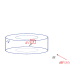
\includegraphics[]{biot_savart}
	\caption{Champ magnétique généré par un élément infinitésimal d'un conducteur
	de densité volumique de courant $\vecj$ en un point $M$ de l'espace.}%
	\label{fig:magneto_biot_savart}
\end{figure}

On considère un conducteur formant un volume $\mathcal{V}$ 
(voir Fig.~\ref{fig:magneto_biot_savart}) parcouru par des charges mobiles 
de densité volumique de charge $\rho$ se déplaçant à la vitesse $\vecv$. Un élément 
infinitésimal $\dV$ de ce circuit centré en $P$ génère en un point $M$ un champ magnétique

\begin{equation*}
	\mathrm{\textbf{d}}\mitbf{B}^P(M) = \dfrac{\mu_0 \rho(P) \dV}
	{4 \pi} \vecv(P) \wedge 
	          \dfrac{\mitbf{PM}}{||PM||^3},
\end{equation*}
où on reconnaît le vecteur densité de courant $\vecj(P) = \rho(P) \vecv(P)$. 
Le champ magnétique
$\vecb$ généré par l'ensemble du circuit en $M$ est alors obtenu en additionnant les 
contributions de chaque élément de ce dernier grâce au principe de superposition
\begin{equation*}
	\vecb(M) = \iiint_{P \in \mathcal{V}} \mathrm{\textbf{d}}\mitbf{B}^P(M)
		 = \iiint_{P \in \mathcal{V}} \dfrac{\mu_0}
		 {4 \pi} \vecj(P) \wedge 
	          \dfrac{\mitbf{PM}}{||PM||^3} \dV
\end{equation*}
On aboutit ainsi à la loi de Biot et Savart.

\begin{defn}[Loi de Biot et Savart]
	Le champ magnétostatique $\vecb(M)$ créé au point $M$ par une distribution
	volumique de courant $\vecj$ ($\ampere \usk \rpsquare \meter$) contenue
	dans un volume $\mathcal{V}$ est
	\begin{equation}
		\vecb(M) = \dfrac{\mu_0}{4 \pi} \iiint_{P \in \mathcal{V}} 
		\dfrac{\vecj(P) \wedge \mitbf{PM}}{||PM||^3} \dV,
	\end{equation}
	où $\mu_0 = \unit{4 \pi \times 10^{-7}}{\tesla \usk \meter \usk \reciprocal
	\ampere}$ est la perméabilité magnétique du vide.

\end{defn}

	Par un raisonnement similaire, on montre que pour une distribution 
	surfacique de courant $\vecj_s$ confinée sur une 
	surface $\mathcal{S}$, cette expression devient
	\begin{equation}
		\vecb(M) = \dfrac{\mu_0}{4 \pi} \iint_{P \in \mathcal{S}} 
		\dfrac{\vecj_s(P) \wedge \mitbf{PM}}{||PM||^3} \mathrm{d}S.
	\end{equation}

	Pour un circuit filiforme $\mathcal{C}$ parcouru par un courant $I$, 
	cette expression devient
	\begin{equation}
		\vecb(M) = \dfrac{\mu_0}{4 \pi} \int_{P \in \mathcal{C}} 
	\dfrac{I \dl \wedge \mitbf{PM}}{||PM||^3}.
	\end{equation}

\begin{exemple}
	On cherche à déterminer le champ magnétique généré par un fil infini $\mathcal{C}$
	parcouru
	par un courant d'intensité $I$ en un point $M$ 
	(voir Fig.~\ref{fig:magneto_spire}). On se place dans un repère cylindrique
	$(0, \er, \etheta, \ez)$. Les points $M$ et $P$ ont pour coordonnées 
	respectives $(r, \theta, 0)$ et $(0, 0, z_P)$.

	Le champ magnétique $\mathrm{\textbf{d}}\vecb^P(M)$ généré par un élément
	$\dl_P$ du fil centré en $P$ s'écrit
	\begin{equation*}
	\mathrm{\textbf{d}}\vecb^P(M) = \dfrac{\mu_0}{4 \pi} 
	              \dfrac{I \dl_P \wedge \mitbf{PM}}{||PM||^3},
	\end{equation*}
	où $\mitbf{PM} = \mitbf{PO} + \mitbf{OM} = - z_P\ez + r\er$. Dans un repère
	cylindrique, un élément infinitésimal $\dl_P$ du fil s'écrit
	$\dl_P = \dz_P \ez$. On a alors
	\begin{equation*}
		\dfrac{\dl_P \wedge \mitbf{PM}}{||PM||^3} = 
		\dfrac{r\dz_P}{||PM||^3}\etheta. 	
	\end{equation*}
	En remarquant que $||PM|| = r/\cos\alpha$, l'expression précédente devient alors
	\begin{equation*}
		\dfrac{r\dz_P}{||PM||^3}\etheta = \dfrac{\cos^3\alpha \dz_P}
		{r^2} \etheta
	\end{equation*}
	De même, on remarque que $z_p = r \tan\alpha$.
	Par différentiation, on obtient donc
	\begin{equation*}
		\dz_P = \mathrm{d}\left[r\tan\alpha\right] = 
		\dfrac{r \mathrm{d}\alpha}{\cos^2\alpha}.
	\end{equation*}
	Finalement,
	\begin{equation*}
		\mathrm{\textbf{d}}\vecb^P(M) = \dfrac{\mu_0 I \cos\alpha}
		{4 \pi r} \mathrm{d}\alpha \etheta.
	\end{equation*}
	Le champ $\vecb(M)$ généré au point $M$ par le fil s'obtient alors
	en utilisant le principe de superposition, ce qui revient à intégrer les champs 
	magnétiques infinitésimaux sur l'ensemble du fil. Pour parcourir l'ensemble du
	fil, $\alpha$ doit varier entre $-\pi/2$ et $\pi/2$. On a alors
	\begin{equation*}
		\boxed{\vecb(M) = \dfrac{\mu_0 I}{4\pi r}
			\times \displaystyle{\int_{-\pi/2}^{\pi/2} 
			\cos\alpha\mathrm{d}\alpha \etheta} =
	\dfrac{\mu_0 I}{2\pi r}\etheta.}
	\end{equation*}
	On obtient un champ magnétique porté par $\etheta$ et donc la norme ne dépend
	que de $r$. Les lignes de ce champ sont des cercles concentriques centrés
	sur le fil. $\vecb$ "tourne" autour du fil.
\end{exemple}
\begin{figure}[h!]
	\centering
	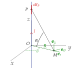
\includegraphics[scale=0.7]{fil}
	\caption{Champ magnétique créé en un point $M$ par un fil parcouru par
	un courant d'intensité $I$.}%
	\label{fig:magneto_spire}
\end{figure}

\begin{defn}[Calcul du champ magnétique par la loi de Biot et Savart]
	Comme nous l'avons vu dans l'exemple précédent, la loi de Biot et Savart
	peut s'avérer utile lorsqu'il s'agit de calculer le champ magnétique 
	$\vecb$ généré par une distribution de courant. Voici en résumé la démarche à suivre
	\begin{enumerate}
		\item Réaliser un schéma du système et choisir un repère adapaté.
		\item Exprimer le petit volume $\dV$, de surface $\mathrm{d}S$
		  ou de longueur $\dl$ dans ce système de coordonnées.
	  \item En multipliant cet élément par le courant ($\vecj$, $\vecj_s$ ou
	    $I$), on obtient le petit élément de courant associé.
	  \item Exprimer le vecteur $\mitbf{PM}$ dans le système de coordonnées
	    choisi.
    	\item En multipliant par $\dfrac{\mu_0}{4 \pi}$ et en faisant le produit 
	  vectoriel par $\dfrac{\mitbf{PM}}{||PM||^3}$, on fabrique le champ
	  élémentaire $\mathrm{\textbf{d}}\vecb^P(M)$ généré en $M$.
	\item Pour calculer $\vecb(M)$, il suffit alors d'intégrer sur la distribution
	  de courant.
	\end{enumerate}
\end{defn}
\section{Équation de la magnétostatique}
On considère un fil parcouru par un courant $I$ dans un
repère cylindrique $(O, \er, \etheta, \ez)$ (voir Fig.~\ref{fig:magneto_spire}). 
Comme vu ci-dessus, le champ
magnétique créé par ce fil en un point $M$ situé à une distance $r$ du fil
est donné par
\begin{equation*}
	\vecb(M) = \dfrac{\mu_0 I}{2 \pi r}\etheta.
\end{equation*}
Comme pour le champ électrostatique, nous allons nous servir de cet exemple simple 
pour retrouver certaines propriétés du champ magnétostatique.

\subsection{Le théorème d'Ampère}
Le théorème d'Ampère est l'équivalent pour le champ magnétostatique $\vecb$
du théorème de Gauss. Il va nous permettre de calculer facilement le champ
magnétostatique généré par une distribution de courants simple.

Les lignes du champ $\vecb$ créé par le fil sont des cercles dont l'axe est le
fil. Nous cherchons donc dans un premier temps à calculer la circulation de $\vecb$ 
sur la ligne de champ $\mathcal{C}$ de rayon $r$ passant par $M$. 
On a bien pris soin au préalable
d'orienter cette dernière. Dans un repère cylindrique, un petit élément $\dl$ de ce 
contour fermé s'écrit $\dl = r \dtheta \etheta$. La circulation de $\vecb$ sur
ce contour s'écrit donc
\begin{equation*}
	\boxed{\displaystyle{\oint_\mathcal{C} \vecb \cdot \dl = 
		\oint_0^{2 \pi} \dfrac{\mu_0 I}{2 \pi r} r\dtheta
	= \mu_0 I.}}
\end{equation*}
On constate que la circulation du champ $\vecb$ le long du circuit $\mathcal{C}$
ne dépend que du courant $I$ que ce dernier enlace. Cette propriété que nous venons
de montrer pour un fil est en fait une propriété générale du champ magnétostatique.

\begin{defn}[Théorème d'Ampère]
	La circulation du champ magnétostatique $\vecb$ le long d'un circuit fermé
	$\mathcal{C}$ est égale au courant \textbf{algébrique} $I_\mathrm{int}$ 
	enlacé par ce dernier multiplié
	par $\mu_0$
	\begin{equation}
		\oint_\mathcal{C} \vecb \cdot \dl = \mu_0 I_\mathrm{int}.
	\end{equation}
	Le contour sur lequel est réalisée l'intégrale est appelé contour d'Ampère.
	Le courant enlacé $I_\mathrm{int}$ est le courant qui traverse une surface 
	orientée
	qui s'appuie sur le contour d'Ampère. L'orientation de la surface 
	se déduit de celle du contour
	grâce à la règle de la main droite ou du tire-bouchon.
\end{defn}

\begin{exemple}
	\begin{minipage}{0.6\linewidth}
	Soit deux fils électriques parcourus par des courants $I_1$ et $I_2$.
	Avec les orientations choisies, le théorème d'Ampère appliqué au 
	contour $\mathcal{C}$ s'écrit
	\begin{equation*}
		\oint_\mathcal{C} \vecb \cdot \dl = \mu_0(I_1 - I_2).
	\end{equation*}
	\end{minipage}
	\hfill
	\begin{minipage}{0.35\linewidth}
		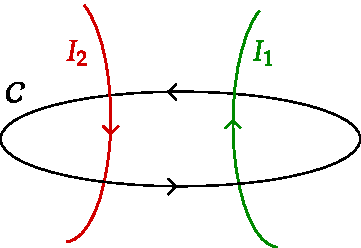
\includegraphics[width=0.8\linewidth]{ampere_ex}
	\end{minipage}

\end{exemple}

Le théorème d'Ampère peut-être traduit sous une forme locale:
appelée \textbf{équation de Maxwell-Ampère}, qui relie alors le champ magnétostatique
au vecteur densité de courant.

\begin{defn}[Équation de Maxwell-Ampère]
	L'équation de Maxwell-Ampère relie le champ magnétostatique $\vecb$
	au vecteur densité de courant $\vecj$
	\begin{equation}
		\rot \vecb = \mu_0 \vecj.
		\label{eq:magneto_ma}
	\end{equation}
	Cette équation est une relation $\textbf{locale}$, elle permet de relier 
	les dérivées spatiales du champ $\vecb$ en un point de l'espace au vecteur
	$\vecj$ en ce même point.
\end{defn}

\subsection{Flux du champ magnétostatique $\vecb$}
On cherche maintenant à calculer la divergence du champ $\vecb$. En coordonnées 
cylindriques, cela donne
\begin{equation*}
	\div \vecb = \dfrac{1}{r}\left(\dd{r B_r}{r} + \dd{B_\theta}{\theta} \right)
	+ \dd{B_z}{z},
\end{equation*}
où $B_r$, $B_\theta$ et $B_z$ sont les composantes de $\vecb$. 
Dans le cas du fil infini, $B_\theta$ est la seule composante non nulle de $\vecb$ 
et elle ne dépend pas
de $\theta$. On a donc
\begin{equation*}
	\div \vecb = 0.
\end{equation*}
Ce résultat se généralise à un champ magnétostatique $\vecb$ quelconque sous
la forme de l'équation de Maxwell-Thomson.

\begin{defn}[Équation de Maxwell-Thomson]
	Un champ magnétique $\vecb$ vérifie toujours
	\begin{equation*}
		\div \vecb = 0.
	\end{equation*}
	Cette relation locale est vérifiée en tout point de l'espace.
\end{defn}

\begin{rem}
La divergence de $\vecb$ étant nulle, l'analyse vectorielle affirme
qu'il est possible dans ce cas de définir un champ vectoriel $\veca$,
défini à un gradient près, tel que $\rot \veca = \vecb$,
appelé le potentiel vecteur.
\end{rem}

Comme l'équation de Maxwell-Ampère, cette équation peut se mettre sous une forme
intégrale, en exprimant le flux du champ magnétique à travers une surface fermée
$\mathcal{S}$.

\begin{defn}[Flux du champ magnétostatique]
	Le flux du champ magnétique $\vecb$ à travers une surface fermée 
	$\mathcal{S}$ est nul
	\begin{equation*}
		\oiint_\mathcal{S} \vecb \cdot \ds = 0.
	\end{equation*}
	On dit que le champ $\vecb$ est à flux conservatif.
\end{defn}

	\begin{minipage}{0.6\linewidth}
	On peut appliquer ce résultat à une surface $\mathcal{S}$ particulière
	constituée d'une portion de tube de champ de section d'entrée $\mathcal{S}_e$,
	de section de sortie $\mathcal{S}_s$ et de section latérale $
	\mathcal{S}_l$. 	
	\end{minipage}
	\hfill
	\begin{minipage}{0.3\linewidth}
	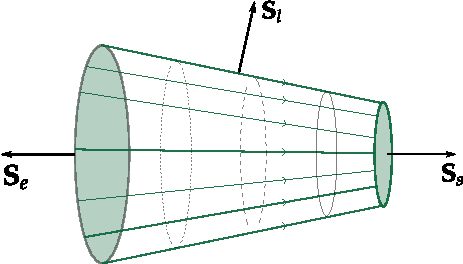
\includegraphics[scale=0.7]{tube}
	\end{minipage}
	\vspace{0.5cm}

\begin{defn}[Tube de champ]
	L'ensemble des lignes de champ s'appuyant sur un contour fermé forme un 
	tube de champ.
\end{defn}
	
	D'après le théorème d'Ampère la flux de $\vecb$ à
	travers cette surface est nul.
	Par définition du tube de champ, l'intégrale sur la surface 
	latérale est nulle. Il reste donc 
	\begin{equation*}
		\iint_\mathcal{S_e} \vecb \cdot \ds_e =
		- \iint_\mathcal{S_s} \vecb \cdot \ds_s 
		\iff
		\displaystyle{\left\lvert\iint_\mathcal{S_e} \vecb \cdot \ds_e\right\rvert =
		\left\lvert\iint_\mathcal{S_s} \vecb \cdot \ds_s\right\rvert}.
	\end{equation*}
	Le flux entrant dans la surface est égal au flux sortant de cette dernière.
	De plus, la surface de sortie étant de taille plus importante que 
	la surface d'entrée, on en conclut que le champ est plus intense
	à l'entrée du tube qu'à la sortie. Le champ $\vecb$ étant à flux
	conservatif, un resserrement des lignes de champs traduit une augmentation
	de l'intensité de ce dernier.

\begin{defn}[Flux conservatif et lignes de champ]
	Le champ magnétique étant à flux conservatif, ses lignes de champs
	se resserrent dans les zones de forte intensité. Inversement, ces dernières
	s'éloignent lorsqu'il devient plus faible
\end{defn}

\section{Étude des lignes de champ de \vecb}
Nous nous intéressons dans cette partie aux propriétés spatiales du champ $\vecb$.
Nous allons voir comment les \textbf{lignes de champ} nous renseignent sur sa répartition 
dans l'espace.

Nous nous intéressons au champ magnétique produit par un solénoïde 
(voir Fig.~\ref{fig:magneto_solenoide}).
Les lignes de champ nous permettent de retrouver quelques propriétés du champ 
magnétostatique énoncées précédemment.

\begin{figure}[htpb]
	\centering
	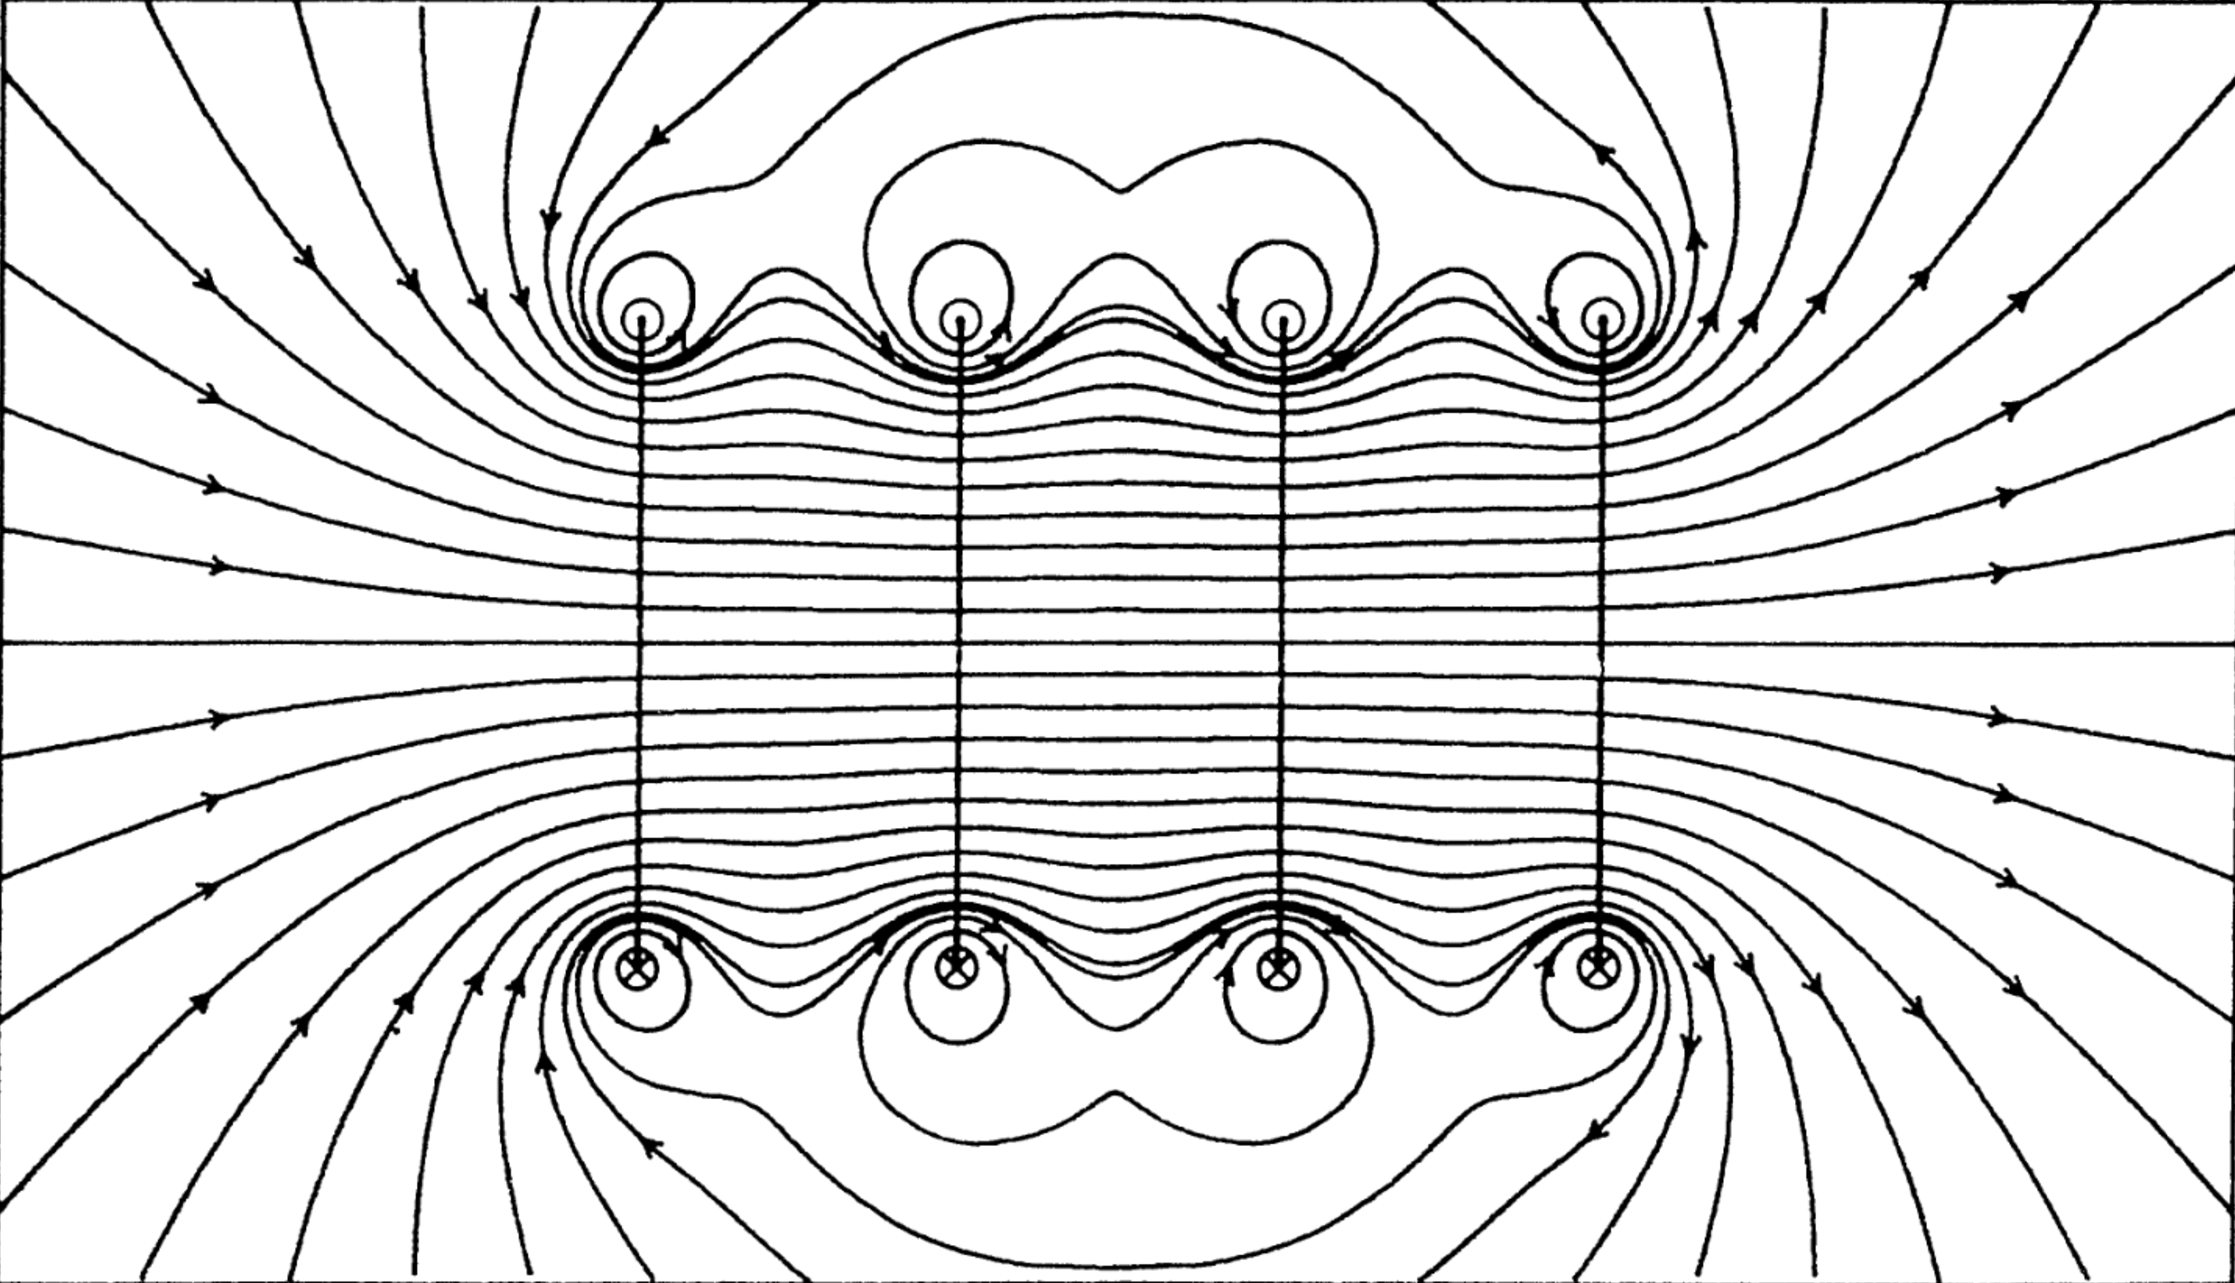
\includegraphics[width=0.7\linewidth]{solenoide}
	\caption{Lignes du champ magnétique généré par un solénoïde constitué de
		4 bobines parcourues dans le même sens par la même intensité.
		Cette figure est extraite de \cite{Gie1985}}%
	\label{fig:magneto_solenoide}
\end{figure}

\begin{enumerate}
	\item On remarque tout d'abord que les lignes de champ 
	  sont des contours fermés qui entourent les fils parcourus par un courant.
	  Cette première observation est une conséquence directe de l'équation
	  de Maxwell-Ampère. L'orientation de ces lignes de champ s'obtient
	  d'ailleurs en considérant le sens du courant dans les fils et en utilisant
	  la règle de la main droite.
      \item La divergence nulle de $\vecb$ est aussi visible sur cette carte de 
	champ. En effet, on constate que les lignes de champ ne convergent/divergent
	pas en un point de l'espace, contrairement au champ électrostatique.
      \item Dans le cas du champ magnétique, le resserrement des lignes de champ
	traduit une augmentation de la norme de ce dernier. On conclut que le champ
	est plus intense à l'intérieur du solénoïde qu'à l'extérieur. De plus, les
	lignes de champ étant parallèles à l'intérieur du solénoïde, on conclut que
	le champ est uniforme.
      \item Grâce aux lignes de champ, on retrouve rapidement les plans de 
	  symétrie et d'antisymétrie du champ magnétique. Le plan médiateur 
	  du solénoïde est par exemple un plan de symétrie du champ magnétique. 
          L'analyse de ces symétries sera utile pour calculer le champ
          magnétique résultant d'une distribution de courant.
\end{enumerate}

\section{Calcul du champ magnétostatique}
\label{sec:calcul_e}
Nous allons voir dans cette partie comment nous pouvons utiliser le théorème d'Ampère
pour calculer le champ magnétostatique $\vecb$ créé 
par une distribution de courants simple. Nous nous intéressons ici à une bobine
torique constituée d'un fil régulièrement bobiné autour d'un tore de section
carré (voir Fig.~\ref{fig:magneto_tore}). Cette bobine est caractérisée par le nombre $N$
total de spires bobinés, son rayon intérieur $R$ 
et sa hauteur $h$. La bobine est parcourue par un courant $I$.

On cherche à déterminer 
l'expression du champ électrique $\vecb$ en un point $M$ de l'espace. Pour ce faire, 
il suffit de suivre le mode d'emploi suivant
\begin{enumerate}
	\item Faire un schéma du système ! C'est absolument indispensable
	  (voir Fig.~\ref{fig:magneto_tore})
	\item Choisir un repère adapté au problème
	\item Étudier les invariances de cette distribution
	\item Étudier les symétries de la distribution de courants à l'origine 
	  du champ magnétostatique
	\item Choisir un contour d'Ampère et appliquer le théorème d'Ampère.
\end{enumerate}

Au vu de la géométrie du système, nous choisissons ici d'utiliser 
un repère cylindrique $(O, \er, \etheta, \ez)$.
Le point $M$ est donc repéré par ses coordonnées $(r, \theta, z)$. Le champ
magnétostatique en $M$ s'écrit de manière générale

\begin{equation}
	\vecb(M) = B_r(M)\er + B_\theta(M)\etheta + B_\varphi(M)\ephi.
	\label{eq:tore}
\end{equation}
Le champ magnétostatique est un vecteur à trois composantes et chaque composante
dépend des coordonnées de $M$. Pour simplifier cette expression, il est intéressant
de considérer les invariances et symétries de la distribution de courant qui génère
le champ $\vecb$.

\begin{figure}
	\centering
	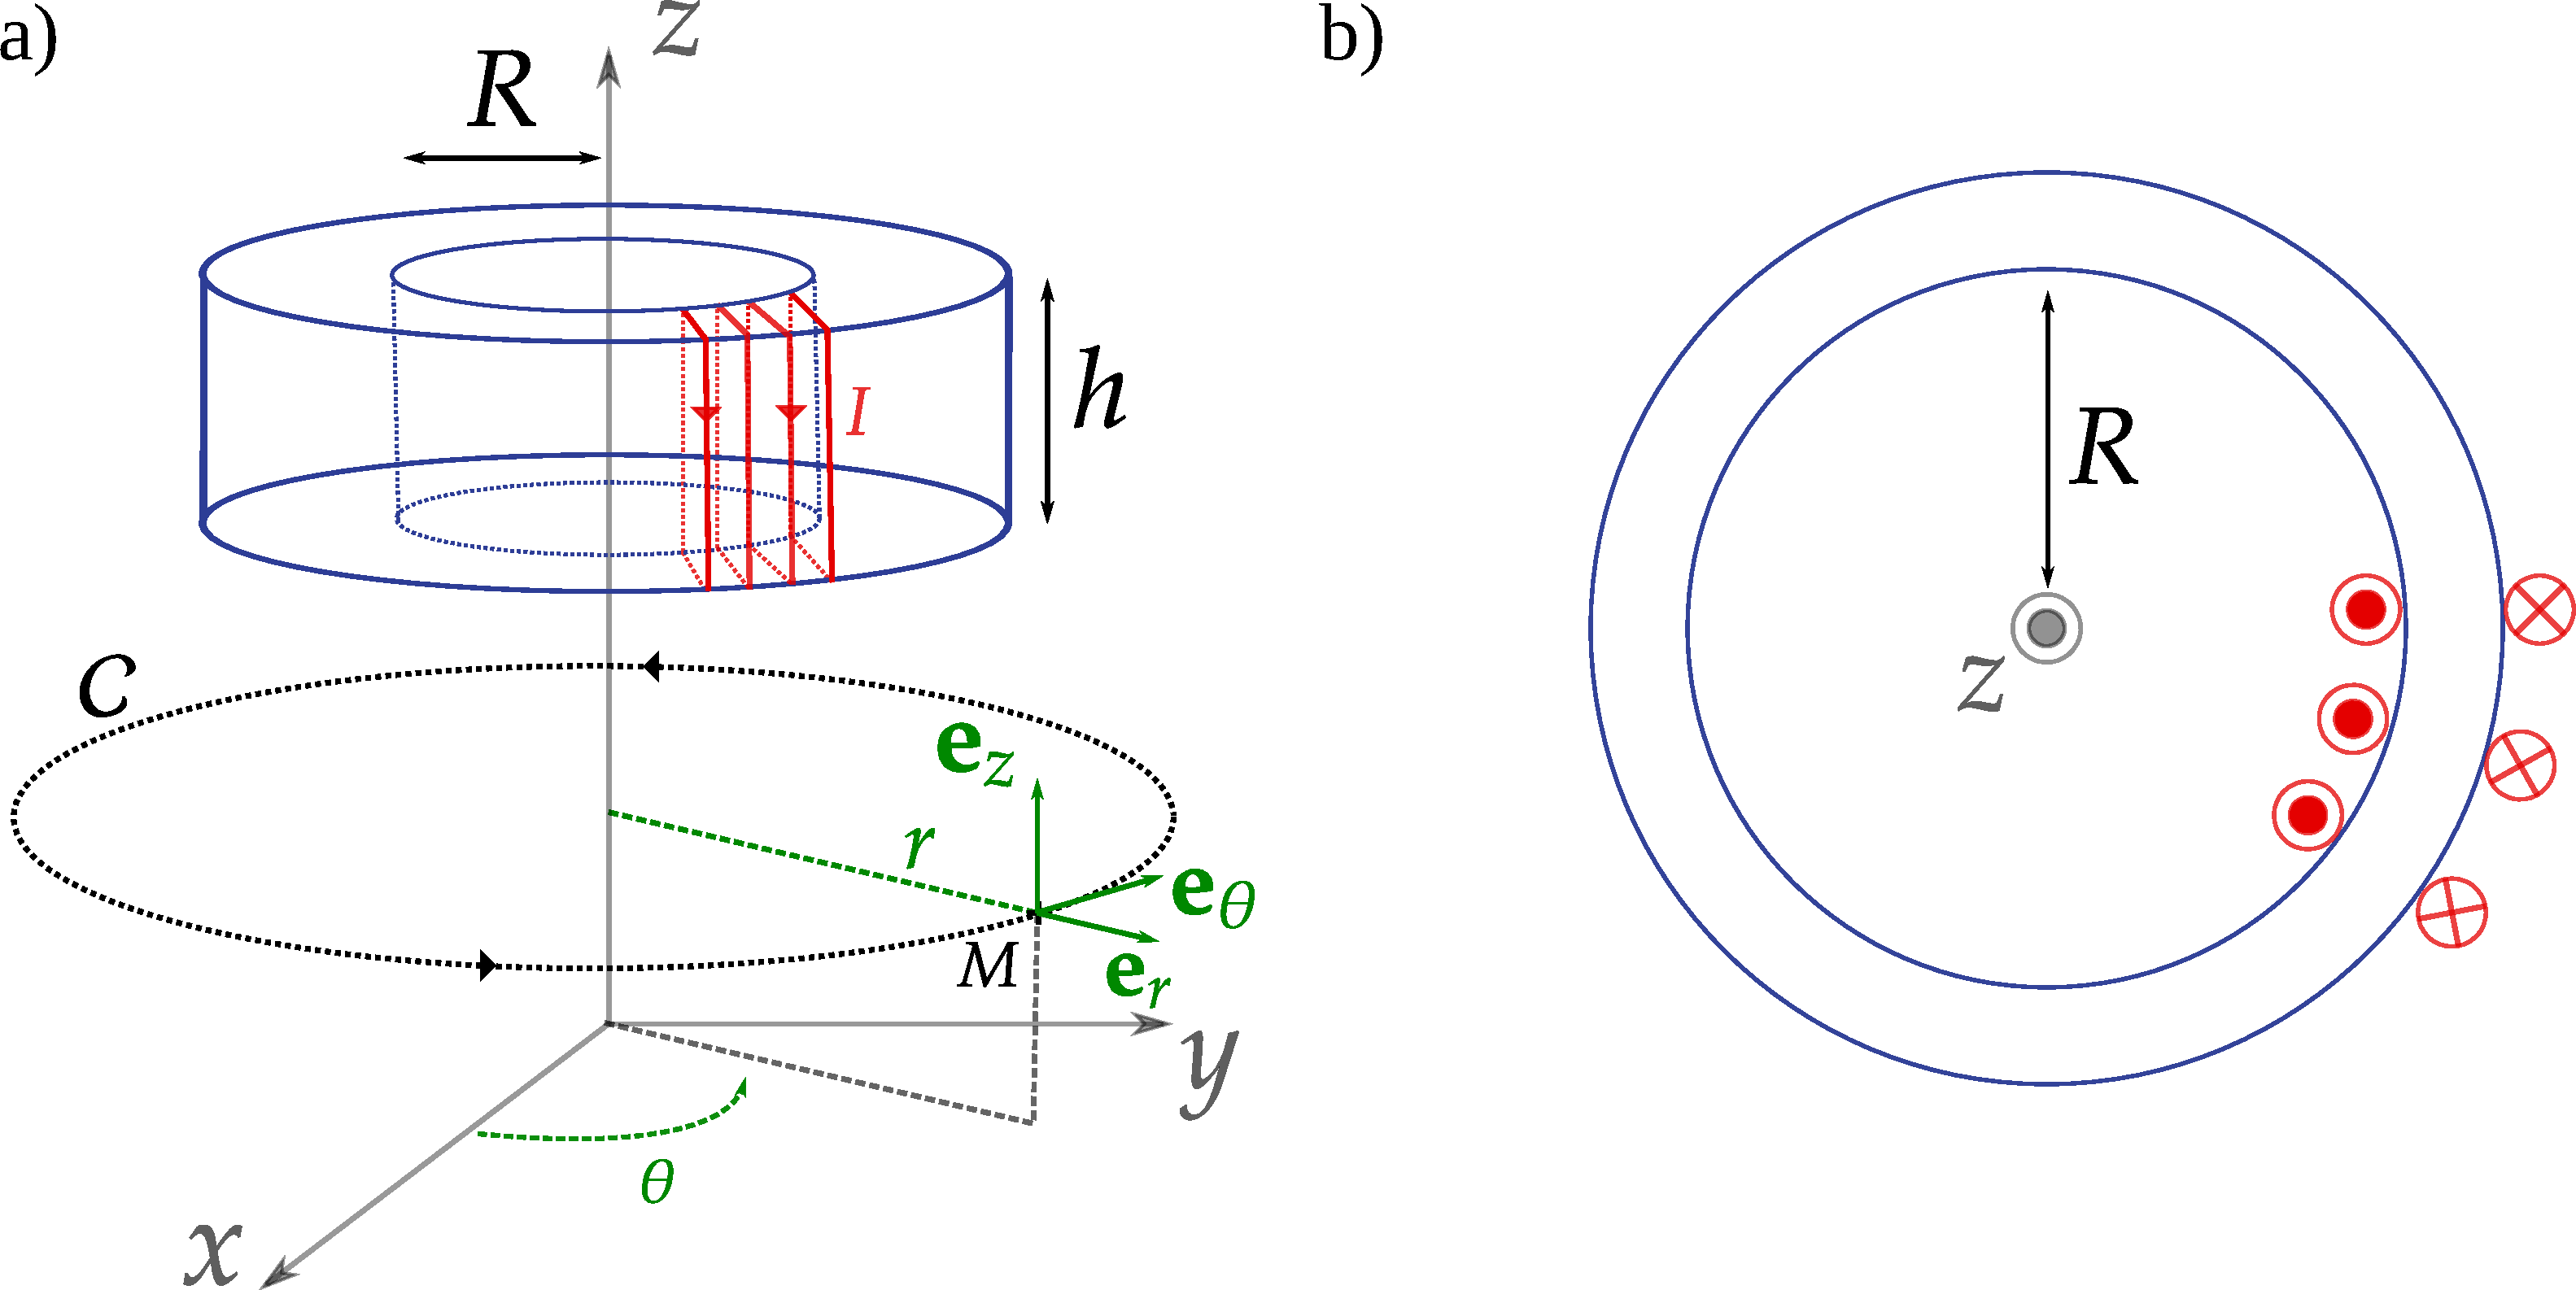
\includegraphics[scale=1]{tore}
	\caption{Bobine torique à gauche et coupe perpendiculaire à $(Oz)$
	de cette bobine à droite.}%
	\label{fig:magneto_tore}
\end{figure}

\subsection{Invariance de la distribution de courants}
On cherche ici à savoir si la distribution de courant est modifiée sous l'effet
d'une translation ou d'une rotation de l'espace. En d'autres termes, on regarde
de quelles variables elle dépend. Étant donné que les spires sont uniformément
répartie sur le tore, on observe que

\begin{itemize}
	\item  si je tourne le tore d'un angle $\Delta \theta$ dans la
	  direction $\etheta$, le problème
	  ne change pas. La distribution de courant est donc invariante 
	  par rotation selon l'angle $\theta$. $\vecb$ \textbf{ne dépend pas de
	  $\mitbf{\theta}$}.
\end{itemize}

Finalement, l'expression~\ref{eq:tore} du champ magnétique se simplifie donc en 

\begin{equation*}
	\boxed{\vecb(M) = B_r(r,z)\er + B_\theta(r,z)\etheta + B_z(r,z)\ez.}
\end{equation*}
\subsection{Symétries de la distribution de courants}

Si on applique ce principe au champ magnétique créé par une distribution 
de courants, cela revient à dire que les symétries de la distributions de 
courants doivent se retrouver dans les symétries du champ magnétique. On en 
déduit les règles suivantes

\begin{defn}[Symétries de $\vecb$ et de la distribution de courant]
\begin{itemize}
  \item si $(\Pi)$ est un plan d'antisymétrie de la distribution de courant et que 
    $M$ appartient à $(\Pi)$, alors obligatoirement $\vecb(M)$ doit 
    appartenir à $(\Pi)$,
  \item si $(\Pi)$ est un plan de symétrie de la distribution de courant 
    et que $M$ appartient à $(\Pi)$, alors obligatoirement $\vecb(M)$ doit 
    être orthogonal à $(\Pi)$.
\end{itemize}
\end{defn}

\begin{rem}
	Le champ magnétostatique $\vecb$ appartient aux plans d'\textbf{antisymétrie}
	de la distribution de courant et non aux plans de symétrie comme
	c'est le cas pour le champ électrostatique. Le vecteur $\vecb$ est 
	qualifié de vecteur axial.
\end{rem}

Pour appliquer ces règles à notre exemple, on détermine les plans de symétrie 
et d'antisymétrie de la distribution de courants auquels 
le point $M$ appartient

\begin{itemize}
	\item le plan $(M, \er, \ez)$ est un plan de symétrie de la distribution
	  de courant. $\vecb(M)$ \textbf{doit être orthogonal à ce plan}.
\end{itemize}

$\vecb(M)$ doit être orthogonal au plan $(M, \er, \ez)$, 
il doit donc être colinéaire à $\etheta$

\begin{framed}
\begin{equation*}
	\vecb(M) = B_\theta(r, z) \etheta.
\end{equation*}
\end{framed}

Nous n'avons imposé aucune condition sur la position de $M$, cette relation est
donc vraie pour tout point $M$ de l'espace. Maintenant que l'expression du 
champ magnétique a été simplifiée au maximum, on cherche à appliquer le théorème
d'Ampère.

\subsection{Application du théorème d'Ampère}
La distribution de courant présente une symétrie de révolution. On choisit comme contour 
d'Ampère un cercle $\mathcal{C}$ de rayon $r$, de centre $O$ et orienté
dans le sens de $\etheta$ qui passe par $M$ 
(voir Fig~\ref{fig:magneto_tore}) et on applique le théorème d'Ampère à ce dernier

\begin{equation*}
	\oint_\mathcal{S} \vecb(M) \cdot \dl = \mu_0 I_\mathrm{int},
	\label{eq:cavite_gauss}
\end{equation*}
où $I_\mathrm{int}$ est la courant enlacé par $\mathcal{C}$. On commence
par déterminer l'expression du membre de gauche. Dans un repère cylindrique,

\begin{equation*}
	\dl = r \dtheta \etheta.
\end{equation*}
On obtient alors
\begin{equation*}
	\oint_\mathcal{C} \vecb(M) \cdot \dl = 
	\oint_\mathcal{C} B(r,z) \etheta \cdot r \dtheta \etheta
	= B(r, z) r \int_0^{2 \pi} \dtheta
	= 2 \pi r B(r,z).
\end{equation*}
On s'intéresse maintenant au terme de droite de l'équation.
Deux cas de figure se présentent:
\begin{itemize}
	\item $M$ est situé dans le tore: le courant enlancé par $\mathcal{C}$ est alors
	  $I_\mathrm{int} = NI$.
       \item $M$ est situé à l'extérieur du tore: le courant enlacé par 
	       $\mathcal{C}$ est donc nul. Soit parce que le contour n'enlace 
	       aucun courant, soit parce qu'il enlace autant de courants positifs
	       que de courants négatifs.
\end{itemize}
Finalement,
\begin{framed}
\begin{itemize}
	\item si $M$ se trouve à l'intérieur du tore, 
	  $\vecb(M) = \dfrac{\mu_0 N I}{2 \pi r} \etheta$.
	\vspace{1em}
\item si $M$ est en dehors du tore, $\vecb(M) = \mitbf{0}$. 
\end{itemize}
\end{framed}
%\nocite{*}
%\putbib[magnetostatique]

%\newpage

%\chapter{Magnétostatique}
\label{chap:magnetostatique}
\section*{Objectifs}%
\label{sec:objectifs}
\begin{itemize}
	\item Connaître les équations qui contrôlent l'évolution spatiale 
	  du champ magnétostatique $\vecb$.
	\item Faire le lien entre ces équations et une carte de champ 
	  magnétique.
	\item Savoir calculer le champ magnétostatique résultant d'une 
	  distribution simple de courants.
\end{itemize}
\newpage
\section*{Introduction}
La magnétostatique étudie les champs magnétiques créés par des courants permanents.
Le plus souvent, on cherche alors à déterminer le champ magnétostatique $\vecb$
qui résulte d'une distribution de courant $\vecj$ connue. Nous nous intéressons
dans ce chapitre au champ magnétique créé par des courants circulants 
dans des conducteurs. Les milieux aimantés seront abordés plus loin dans le cours.

\section{La force de Lorentz}%
L'interaction entre deux particules immobiles a permis de définir la force de 
Coulomb dans le chapitre~\ref{chap:electrostatique}. Cette interaction 
électrostatique ne suffit plus lorsqu'il s'agit de décrire la dynamique de 
charges en mouvement. En 1895, le physicien néerlandais Hendrick Antoon Lorentz
propose alors l'ajout d'un second terme à la force coulombienne qui fait apparaître
la champ magnétostatique $\vecb$. 

\begin{defn}[Champ magnétostatique]
	Au même titre que le champ électrostatique, le champ magnétique $\vecb$
	est un champ vectoriel. Il est généré par une distribution de courant ou 
	par un aimant. Il s'exprime en tesla, noté $\tesla$ ($\kilogram \usk
	\rpsquare \second \reciprocal \ampere$ en SI). On rappelle quelques ordres de
	grandeur du champ magnétique
	
	\begin{center}
	\begin{tabular}{l|l}
		\textbf{Dispositif} 	& $\vecb (\tesla)$ \\ \hline
		Champ magnétique terrestre à la surface & $47 \times 10^{-6}$ \\
		Champ créé à $\unit{1}{\centi \meter}$ d'un fil parcouru par 
		un courant de $\unit{10}{\ampere}$
								 & $2 \times 10^{-5}$ \\
		Champ créé à $\unit{1}{\milli \meter}$ d'un aimant permanent& $0.1 - 1$ \\
		Électroaimant & $10 - 100$ \\
		Étoile à neutrons en surface & $10^{11}$\\
	\end{tabular}
	\end{center}
Le champ magnétique vérifie lui aussi le principe de superposition.
\end{defn}

\begin{defn}[Force de Lorentz]
Une particule de charge $q$ se déplaçant à la vitesse $\vecv$ dans un champ magnétique
$\vecb$, subit une force appelée force de Lorentz
\begin{equation}
	\vecf = q\vecv \wedge \vecb.
\end{equation}
Cette force est donc toujours orthogonale à la vitesse de la particule.
Contrairement à la force électrostatique, la force magnétique n'entraîne donc pas 
de variation de la vitesse de la particule, elle permet seulement de dévier sa 
trajectoire. En effet, la puissance magnétique $\mathcal{P}$ vaut
\begin{equation*}
	\mathcal{P} = \vecf \cdot \vecv = (q\vecv \wedge \vecb) \cdot \vecv = 0.
\end{equation*}
La force magnétique ne permet donc pas de mettre une particule chargée en mouvement.
\end{defn}

Comme pour la force électrostatique, le poids d'une particule chargée est bien souvent 
négligeable devant celui de la force de Lorentz. Pour illustrer cela, prenons le 
cas d'un électron de masse $m_e = \unit{9.1 \times 10^{-31}}{\kilogram}$ et de
charge $q = \unit{1.6 \times 10^{-19}}{\coulomb}$ se déplaçant à une vitesse
$v = \unit{10^5}{\meter \usk \reciprocal \second}$ dans un champ magnétique uniforme
$B = \unit{1}{\tesla}$. On trouve alors
\begin{equation*}
	\dfrac{mg}{qvB} \approx 10^{-15}.
\end{equation*}
On peut alors toujours négliger le poids d'une particule chargée
devant la force de Lorentz.

\begin{exemple}
	On s'intéresse ici au mouvement d'un électron de charge $-e$ et de 
	masse $m$ dans un 
	champ magnétique uniforme $\vecb$ (voir Fig.~\ref{fig:magneto_cyclotron}). 
	La vitesse initiale $\vecv_0$ de la particule est orthogonale au champ
	$\vecb$. La particule est donc soumise à la force de Lorentz et à son
	poids que nous négligeons ici. 
	
	Expérimentalement, on constate que la trajectoire 
	de la particule est circulaire. La force de Lorentz ne travaillant pas, 
	la norme de la vitesse reste en tout temps égale à $v_0$. Le mouvement de la 
	particule est donc uniforme et circulaire.
	
	On se place dans
	un référentiel polaire $(O, \er, \etheta)$. La position de la particule
	est donc repérée par ses coordonnées $(r, \theta)$. L'application du principe
	fondamental de la dynamique à la particule dans le référentiel du
	laboratoire supposé galiléen donne
	\begin{equation*}
		m \dot{\vecv} = q \vecv \wedge \vecb,
	\end{equation*}
	où la notation $\dot{v}$ est utilisée pour la dérivée temporelle.
	Dans un référentiel polaire et pour un mouvement circulaire uniforme, 
	$\vecv = r\dot{\theta} \etheta = v_0 \etheta$ 
	et $\dot{\vecv} = - v_0^2/r\er$. On obtient donc
	\begin{equation*}
		m \dfrac{v_0^2}{r}\er = -e v_0 \etheta \wedge \ez =e v_0 B \er \iff 
		\dot{\theta} = \dfrac{eB}{m}
	\end{equation*}
	L'électron suit donc un mouvement circulaire uniforme à la vitesse angulaire
	$eB/m$ appelée pulsation cyclotron. Dans le cyclotron de University of Michigan,
	le champ magnétique vaut $B = \unit{0.10}{\tesla}$, ce qui donne une pulsation de 
	$\unit{1.7 \times 10^{10}}{\rad \usk \reciprocal \second}$ pour un électron.

\end{exemple}
\begin{figure}[h!]
	\centering
	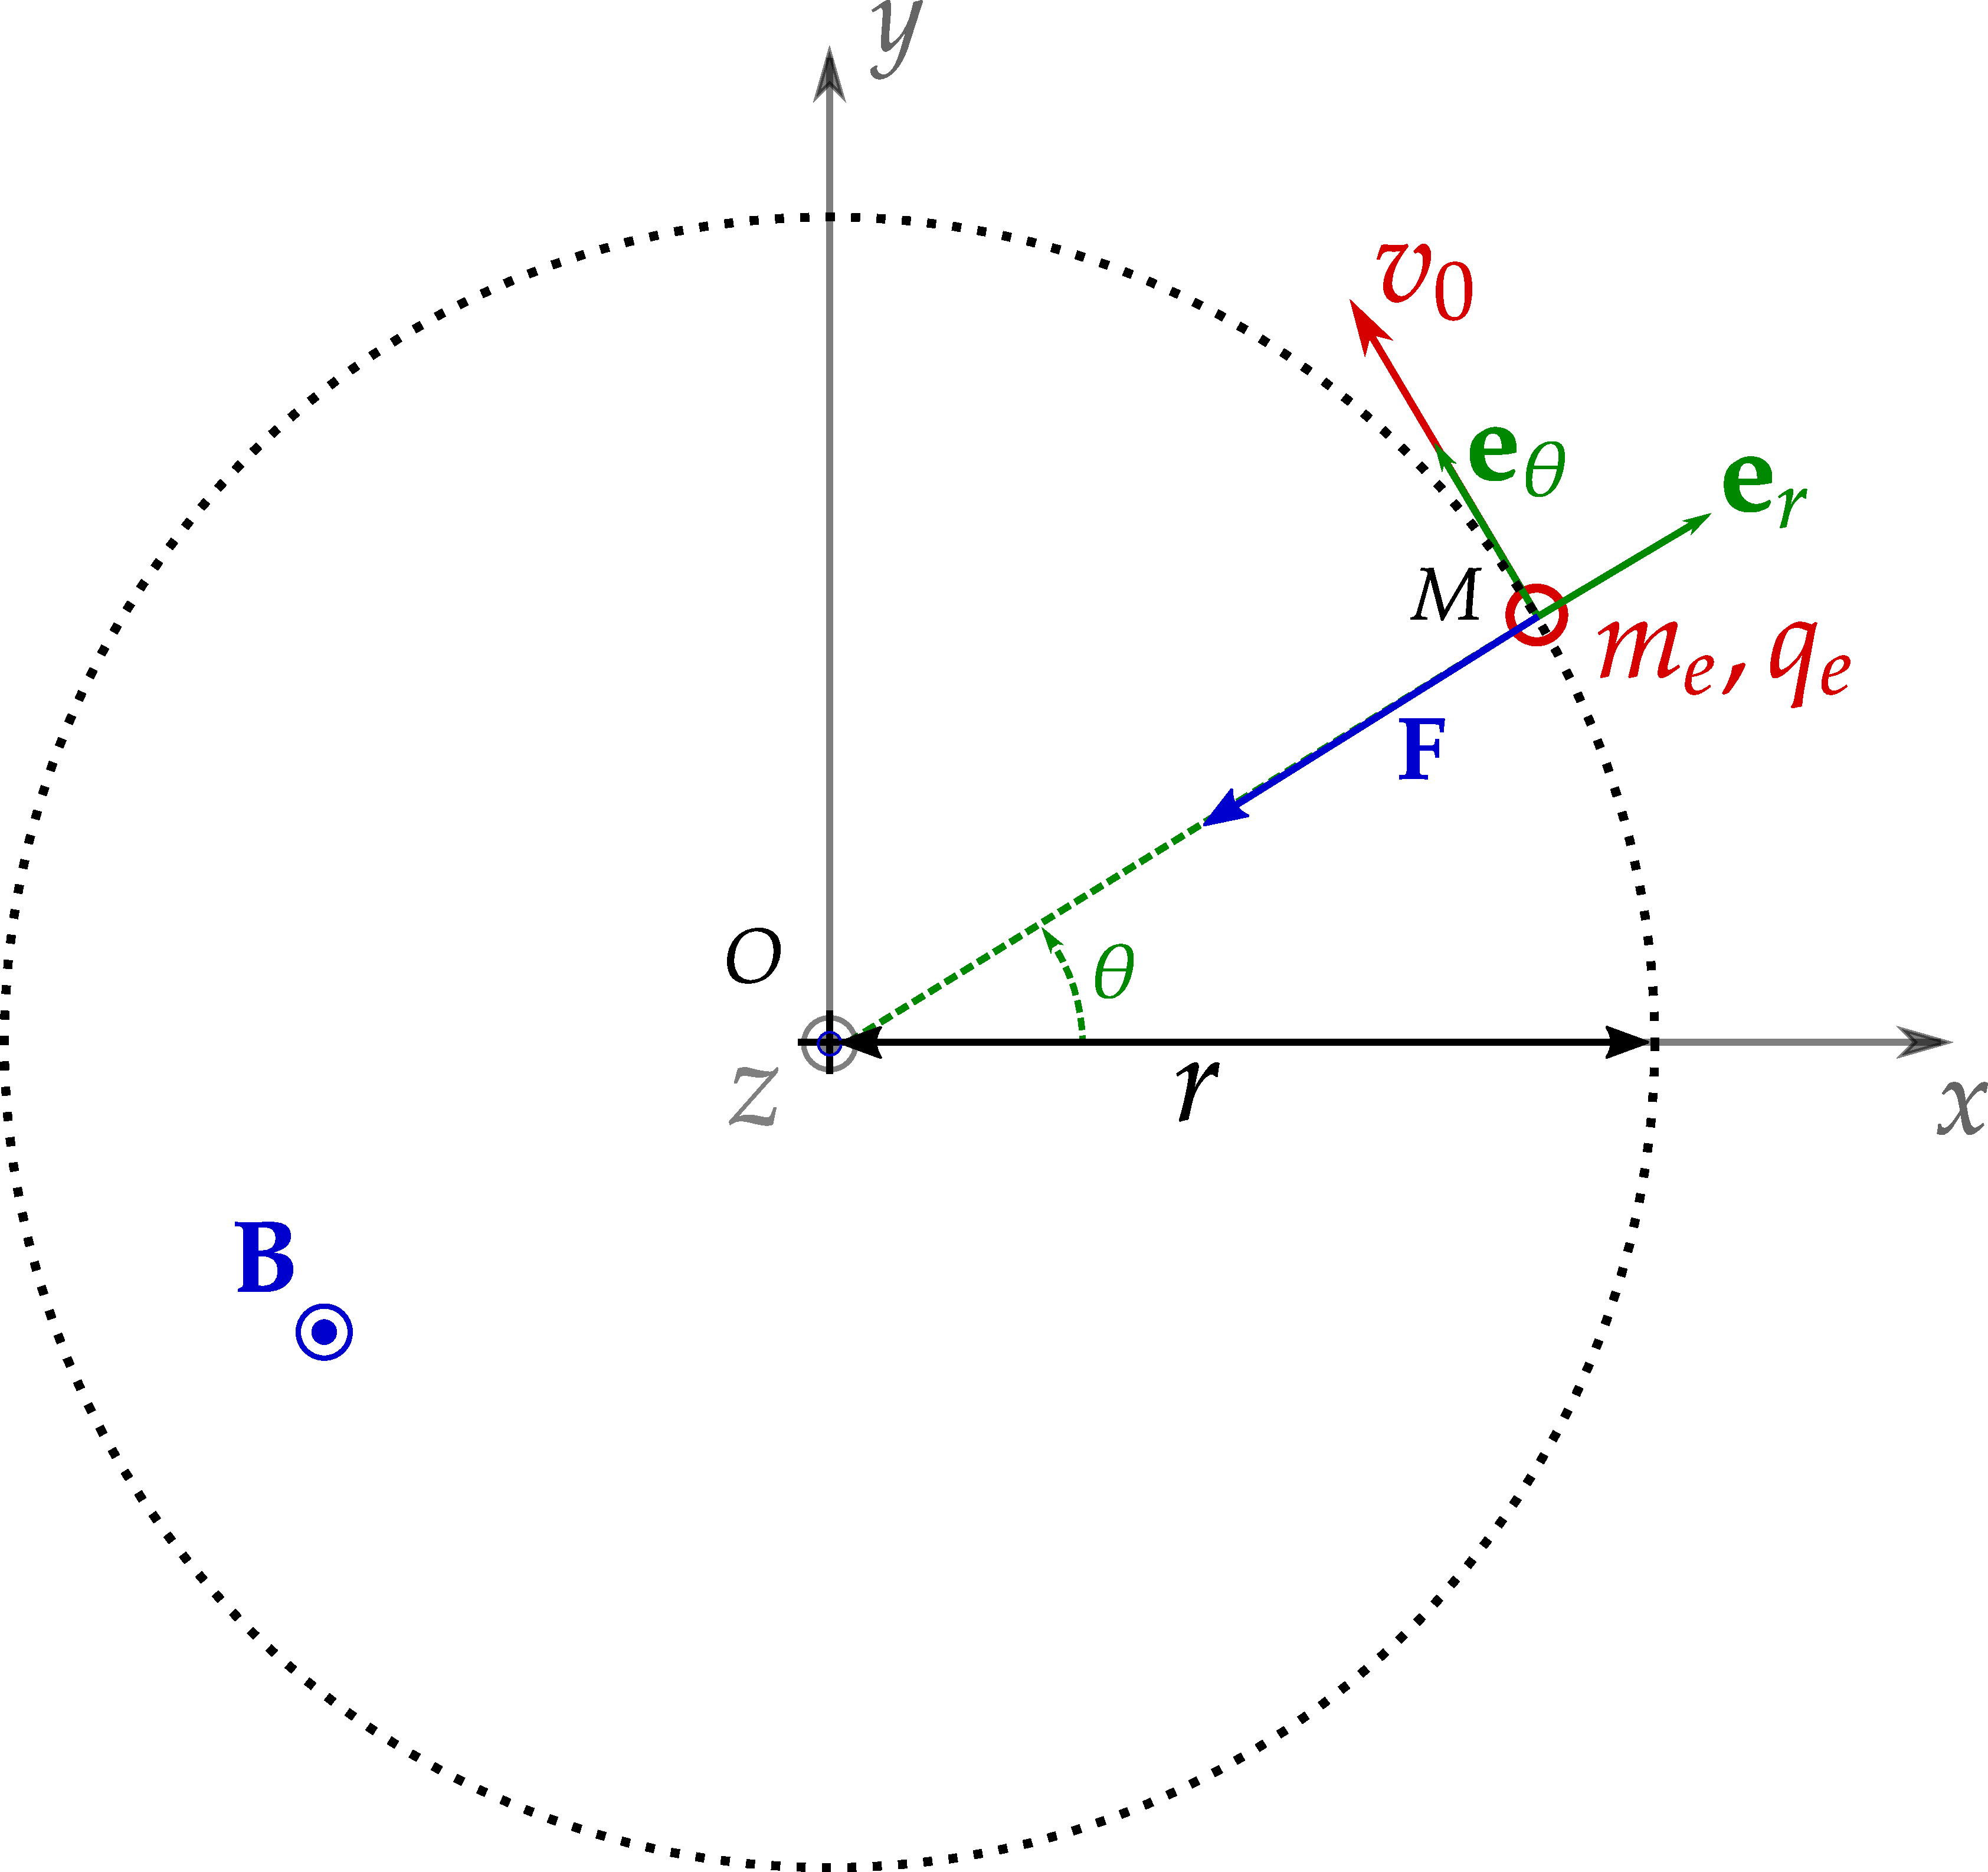
\includegraphics[scale=0.75]{cyclotron}
	\caption{Trajectoire d'un électron dans un champ magnétique uniforme.}%
	\label{fig:magneto_cyclotron}
\end{figure}

\section{La loi de Biot et Savart}
De la même manière que pour le champ électrostatique, nous
commençons par définir le champ magnétique généré par une charge ponctuelle. 
Soit une charge ponctuelle $q$ en un point $P$ de l'espace se déplaçant 
à la vitesse $\vecv$ dans le référentiel du laboratoire. Expérimentalement,
on observe que cette particule génère
en un point $M$ un champ magnétique $\vecb(M)$ tel que

\begin{equation*}
	\vecb(M) = \dfrac{\mu_0 q}{4 \pi} \vecv \wedge \dfrac{\mitbf{PM}}{||PM||^3},
\end{equation*}
où $\mu_0 = \unit{4 \pi \times 10^{-7}}{\tesla \usk \meter \usk \reciprocal 
\ampere}.$

\begin{figure}[h!]
	\centering
	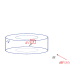
\includegraphics[]{biot_savart}
	\caption{Champ magnétique généré par un élément infinitésimal d'un conducteur
	de densité volumique de courant $\vecj$ en un point $M$ de l'espace.}%
	\label{fig:magneto_biot_savart}
\end{figure}

On considère un conducteur formant un volume $\mathcal{V}$ 
(voir Fig.~\ref{fig:magneto_biot_savart}) parcouru par des charges mobiles 
de densité volumique de charge $\rho$ se déplaçant à la vitesse $\vecv$. Un élément 
infinitésimal $\dV$ de ce circuit centré en $P$ génère en un point $M$ un champ magnétique

\begin{equation*}
	\mathrm{\textbf{d}}\mitbf{B}^P(M) = \dfrac{\mu_0 \rho(P) \dV}
	{4 \pi} \vecv(P) \wedge 
	          \dfrac{\mitbf{PM}}{||PM||^3},
\end{equation*}
où on reconnaît le vecteur densité de courant $\vecj(P) = \rho(P) \vecv(P)$. 
Le champ magnétique
$\vecb$ généré par l'ensemble du circuit en $M$ est alors obtenu en additionnant les 
contributions de chaque élément de ce dernier grâce au principe de superposition
\begin{equation*}
	\vecb(M) = \iiint_{P \in \mathcal{V}} \mathrm{\textbf{d}}\mitbf{B}^P(M)
		 = \iiint_{P \in \mathcal{V}} \dfrac{\mu_0}
		 {4 \pi} \vecj(P) \wedge 
	          \dfrac{\mitbf{PM}}{||PM||^3} \dV
\end{equation*}
On aboutit ainsi à la loi de Biot et Savart.

\begin{defn}[Loi de Biot et Savart]
	Le champ magnétostatique $\vecb(M)$ créé au point $M$ par une distribution
	volumique de courant $\vecj$ ($\ampere \usk \rpsquare \meter$) contenue
	dans un volume $\mathcal{V}$ est
	\begin{equation}
		\vecb(M) = \dfrac{\mu_0}{4 \pi} \iiint_{P \in \mathcal{V}} 
		\dfrac{\vecj(P) \wedge \mitbf{PM}}{||PM||^3} \dV,
	\end{equation}
	où $\mu_0 = \unit{4 \pi \times 10^{-7}}{\tesla \usk \meter \usk \reciprocal
	\ampere}$ est la perméabilité magnétique du vide.

\end{defn}

	Par un raisonnement similaire, on montre que pour une distribution 
	surfacique de courant $\vecj_s$ confinée sur une 
	surface $\mathcal{S}$, cette expression devient
	\begin{equation}
		\vecb(M) = \dfrac{\mu_0}{4 \pi} \iint_{P \in \mathcal{S}} 
		\dfrac{\vecj_s(P) \wedge \mitbf{PM}}{||PM||^3} \mathrm{d}S.
	\end{equation}

	Pour un circuit filiforme $\mathcal{C}$ parcouru par un courant $I$, 
	cette expression devient
	\begin{equation}
		\vecb(M) = \dfrac{\mu_0}{4 \pi} \int_{P \in \mathcal{C}} 
	\dfrac{I \dl \wedge \mitbf{PM}}{||PM||^3}.
	\end{equation}

\begin{exemple}
	On cherche à déterminer le champ magnétique généré par un fil infini $\mathcal{C}$
	parcouru
	par un courant d'intensité $I$ en un point $M$ 
	(voir Fig.~\ref{fig:magneto_spire}). On se place dans un repère cylindrique
	$(0, \er, \etheta, \ez)$. Les points $M$ et $P$ ont pour coordonnées 
	respectives $(r, \theta, 0)$ et $(0, 0, z_P)$.

	Le champ magnétique $\mathrm{\textbf{d}}\vecb^P(M)$ généré par un élément
	$\dl_P$ du fil centré en $P$ s'écrit
	\begin{equation*}
	\mathrm{\textbf{d}}\vecb^P(M) = \dfrac{\mu_0}{4 \pi} 
	              \dfrac{I \dl_P \wedge \mitbf{PM}}{||PM||^3},
	\end{equation*}
	où $\mitbf{PM} = \mitbf{PO} + \mitbf{OM} = - z_P\ez + r\er$. Dans un repère
	cylindrique, un élément infinitésimal $\dl_P$ du fil s'écrit
	$\dl_P = \dz_P \ez$. On a alors
	\begin{equation*}
		\dfrac{\dl_P \wedge \mitbf{PM}}{||PM||^3} = 
		\dfrac{r\dz_P}{||PM||^3}\etheta. 	
	\end{equation*}
	En remarquant que $||PM|| = r/\cos\alpha$, l'expression précédente devient alors
	\begin{equation*}
		\dfrac{r\dz_P}{||PM||^3}\etheta = \dfrac{\cos^3\alpha \dz_P}
		{r^2} \etheta
	\end{equation*}
	De même, on remarque que $z_p = r \tan\alpha$.
	Par différentiation, on obtient donc
	\begin{equation*}
		\dz_P = \mathrm{d}\left[r\tan\alpha\right] = 
		\dfrac{r \mathrm{d}\alpha}{\cos^2\alpha}.
	\end{equation*}
	Finalement,
	\begin{equation*}
		\mathrm{\textbf{d}}\vecb^P(M) = \dfrac{\mu_0 I \cos\alpha}
		{4 \pi r} \mathrm{d}\alpha \etheta.
	\end{equation*}
	Le champ $\vecb(M)$ généré au point $M$ par le fil s'obtient alors
	en utilisant le principe de superposition, ce qui revient à intégrer les champs 
	magnétiques infinitésimaux sur l'ensemble du fil. Pour parcourir l'ensemble du
	fil, $\alpha$ doit varier entre $-\pi/2$ et $\pi/2$. On a alors
	\begin{equation*}
		\boxed{\vecb(M) = \dfrac{\mu_0 I}{4\pi r}
			\times \displaystyle{\int_{-\pi/2}^{\pi/2} 
			\cos\alpha\mathrm{d}\alpha \etheta} =
	\dfrac{\mu_0 I}{2\pi r}\etheta.}
	\end{equation*}
	On obtient un champ magnétique porté par $\etheta$ et donc la norme ne dépend
	que de $r$. Les lignes de ce champ sont des cercles concentriques centrés
	sur le fil. $\vecb$ "tourne" autour du fil.
\end{exemple}
\begin{figure}[h!]
	\centering
	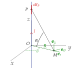
\includegraphics[scale=0.7]{fil}
	\caption{Champ magnétique créé en un point $M$ par un fil parcouru par
	un courant d'intensité $I$.}%
	\label{fig:magneto_spire}
\end{figure}

\begin{defn}[Calcul du champ magnétique par la loi de Biot et Savart]
	Comme nous l'avons vu dans l'exemple précédent, la loi de Biot et Savart
	peut s'avérer utile lorsqu'il s'agit de calculer le champ magnétique 
	$\vecb$ généré par une distribution de courant. Voici en résumé la démarche à suivre
	\begin{enumerate}
		\item Réaliser un schéma du système et choisir un repère adapaté.
		\item Exprimer le petit volume $\dV$, de surface $\mathrm{d}S$
		  ou de longueur $\dl$ dans ce système de coordonnées.
	  \item En multipliant cet élément par le courant ($\vecj$, $\vecj_s$ ou
	    $I$), on obtient le petit élément de courant associé.
	  \item Exprimer le vecteur $\mitbf{PM}$ dans le système de coordonnées
	    choisi.
    	\item En multipliant par $\dfrac{\mu_0}{4 \pi}$ et en faisant le produit 
	  vectoriel par $\dfrac{\mitbf{PM}}{||PM||^3}$, on fabrique le champ
	  élémentaire $\mathrm{\textbf{d}}\vecb^P(M)$ généré en $M$.
	\item Pour calculer $\vecb(M)$, il suffit alors d'intégrer sur la distribution
	  de courant.
	\end{enumerate}
\end{defn}
\section{Équation de la magnétostatique}
On considère un fil parcouru par un courant $I$ dans un
repère cylindrique $(O, \er, \etheta, \ez)$ (voir Fig.~\ref{fig:magneto_spire}). 
Comme vu ci-dessus, le champ
magnétique créé par ce fil en un point $M$ situé à une distance $r$ du fil
est donné par
\begin{equation*}
	\vecb(M) = \dfrac{\mu_0 I}{2 \pi r}\etheta.
\end{equation*}
Comme pour le champ électrostatique, nous allons nous servir de cet exemple simple 
pour retrouver certaines propriétés du champ magnétostatique.

\subsection{Le théorème d'Ampère}
Le théorème d'Ampère est l'équivalent pour le champ magnétostatique $\vecb$
du théorème de Gauss. Il va nous permettre de calculer facilement le champ
magnétostatique généré par une distribution de courants simple.

Les lignes du champ $\vecb$ créé par le fil sont des cercles dont l'axe est le
fil. Nous cherchons donc dans un premier temps à calculer la circulation de $\vecb$ 
sur la ligne de champ $\mathcal{C}$ de rayon $r$ passant par $M$. 
On a bien pris soin au préalable
d'orienter cette dernière. Dans un repère cylindrique, un petit élément $\dl$ de ce 
contour fermé s'écrit $\dl = r \dtheta \etheta$. La circulation de $\vecb$ sur
ce contour s'écrit donc
\begin{equation*}
	\boxed{\displaystyle{\oint_\mathcal{C} \vecb \cdot \dl = 
		\oint_0^{2 \pi} \dfrac{\mu_0 I}{2 \pi r} r\dtheta
	= \mu_0 I.}}
\end{equation*}
On constate que la circulation du champ $\vecb$ le long du circuit $\mathcal{C}$
ne dépend que du courant $I$ que ce dernier enlace. Cette propriété que nous venons
de montrer pour un fil est en fait une propriété générale du champ magnétostatique.

\begin{defn}[Théorème d'Ampère]
	La circulation du champ magnétostatique $\vecb$ le long d'un circuit fermé
	$\mathcal{C}$ est égale au courant \textbf{algébrique} $I_\mathrm{int}$ 
	enlacé par ce dernier multiplié
	par $\mu_0$
	\begin{equation}
		\oint_\mathcal{C} \vecb \cdot \dl = \mu_0 I_\mathrm{int}.
	\end{equation}
	Le contour sur lequel est réalisée l'intégrale est appelé contour d'Ampère.
	Le courant enlacé $I_\mathrm{int}$ est le courant qui traverse une surface 
	orientée
	qui s'appuie sur le contour d'Ampère. L'orientation de la surface 
	se déduit de celle du contour
	grâce à la règle de la main droite ou du tire-bouchon.
\end{defn}

\begin{exemple}
	\begin{minipage}{0.6\linewidth}
	Soit deux fils électriques parcourus par des courants $I_1$ et $I_2$.
	Avec les orientations choisies, le théorème d'Ampère appliqué au 
	contour $\mathcal{C}$ s'écrit
	\begin{equation*}
		\oint_\mathcal{C} \vecb \cdot \dl = \mu_0(I_1 - I_2).
	\end{equation*}
	\end{minipage}
	\hfill
	\begin{minipage}{0.35\linewidth}
		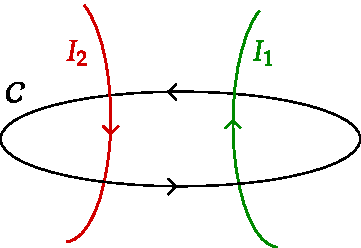
\includegraphics[width=0.8\linewidth]{ampere_ex}
	\end{minipage}

\end{exemple}

Le théorème d'Ampère peut-être traduit sous une forme locale:
appelée \textbf{équation de Maxwell-Ampère}, qui relie alors le champ magnétostatique
au vecteur densité de courant.

\begin{defn}[Équation de Maxwell-Ampère]
	L'équation de Maxwell-Ampère relie le champ magnétostatique $\vecb$
	au vecteur densité de courant $\vecj$
	\begin{equation}
		\rot \vecb = \mu_0 \vecj.
		\label{eq:magneto_ma}
	\end{equation}
	Cette équation est une relation $\textbf{locale}$, elle permet de relier 
	les dérivées spatiales du champ $\vecb$ en un point de l'espace au vecteur
	$\vecj$ en ce même point.
\end{defn}

\subsection{Flux du champ magnétostatique $\vecb$}
On cherche maintenant à calculer la divergence du champ $\vecb$. En coordonnées 
cylindriques, cela donne
\begin{equation*}
	\div \vecb = \dfrac{1}{r}\left(\dd{r B_r}{r} + \dd{B_\theta}{\theta} \right)
	+ \dd{B_z}{z},
\end{equation*}
où $B_r$, $B_\theta$ et $B_z$ sont les composantes de $\vecb$. 
Dans le cas du fil infini, $B_\theta$ est la seule composante non nulle de $\vecb$ 
et elle ne dépend pas
de $\theta$. On a donc
\begin{equation*}
	\div \vecb = 0.
\end{equation*}
Ce résultat se généralise à un champ magnétostatique $\vecb$ quelconque sous
la forme de l'équation de Maxwell-Thomson.

\begin{defn}[Équation de Maxwell-Thomson]
	Un champ magnétique $\vecb$ vérifie toujours
	\begin{equation*}
		\div \vecb = 0.
	\end{equation*}
	Cette relation locale est vérifiée en tout point de l'espace.
\end{defn}

\begin{rem}
La divergence de $\vecb$ étant nulle, l'analyse vectorielle affirme
qu'il est possible dans ce cas de définir un champ vectoriel $\veca$,
défini à un gradient près, tel que $\rot \veca = \vecb$,
appelé le potentiel vecteur.
\end{rem}

Comme l'équation de Maxwell-Ampère, cette équation peut se mettre sous une forme
intégrale, en exprimant le flux du champ magnétique à travers une surface fermée
$\mathcal{S}$.

\begin{defn}[Flux du champ magnétostatique]
	Le flux du champ magnétique $\vecb$ à travers une surface fermée 
	$\mathcal{S}$ est nul
	\begin{equation*}
		\oiint_\mathcal{S} \vecb \cdot \ds = 0.
	\end{equation*}
	On dit que le champ $\vecb$ est à flux conservatif.
\end{defn}

	\begin{minipage}{0.6\linewidth}
	On peut appliquer ce résultat à une surface $\mathcal{S}$ particulière
	constituée d'une portion de tube de champ de section d'entrée $\mathcal{S}_e$,
	de section de sortie $\mathcal{S}_s$ et de section latérale $
	\mathcal{S}_l$. 	
	\end{minipage}
	\hfill
	\begin{minipage}{0.3\linewidth}
	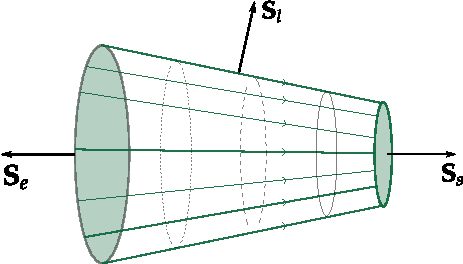
\includegraphics[scale=0.7]{tube}
	\end{minipage}
	\vspace{0.5cm}

\begin{defn}[Tube de champ]
	L'ensemble des lignes de champ s'appuyant sur un contour fermé forme un 
	tube de champ.
\end{defn}
	
	D'après le théorème d'Ampère la flux de $\vecb$ à
	travers cette surface est nul.
	Par définition du tube de champ, l'intégrale sur la surface 
	latérale est nulle. Il reste donc 
	\begin{equation*}
		\iint_\mathcal{S_e} \vecb \cdot \ds_e =
		- \iint_\mathcal{S_s} \vecb \cdot \ds_s 
		\iff
		\displaystyle{\left\lvert\iint_\mathcal{S_e} \vecb \cdot \ds_e\right\rvert =
		\left\lvert\iint_\mathcal{S_s} \vecb \cdot \ds_s\right\rvert}.
	\end{equation*}
	Le flux entrant dans la surface est égal au flux sortant de cette dernière.
	De plus, la surface de sortie étant de taille plus importante que 
	la surface d'entrée, on en conclut que le champ est plus intense
	à l'entrée du tube qu'à la sortie. Le champ $\vecb$ étant à flux
	conservatif, un resserrement des lignes de champs traduit une augmentation
	de l'intensité de ce dernier.

\begin{defn}[Flux conservatif et lignes de champ]
	Le champ magnétique étant à flux conservatif, ses lignes de champs
	se resserrent dans les zones de forte intensité. Inversement, ces dernières
	s'éloignent lorsqu'il devient plus faible
\end{defn}

\section{Étude des lignes de champ de \vecb}
Nous nous intéressons dans cette partie aux propriétés spatiales du champ $\vecb$.
Nous allons voir comment les \textbf{lignes de champ} nous renseignent sur sa répartition 
dans l'espace.

Nous nous intéressons au champ magnétique produit par un solénoïde 
(voir Fig.~\ref{fig:magneto_solenoide}).
Les lignes de champ nous permettent de retrouver quelques propriétés du champ 
magnétostatique énoncées précédemment.

\begin{figure}[htpb]
	\centering
	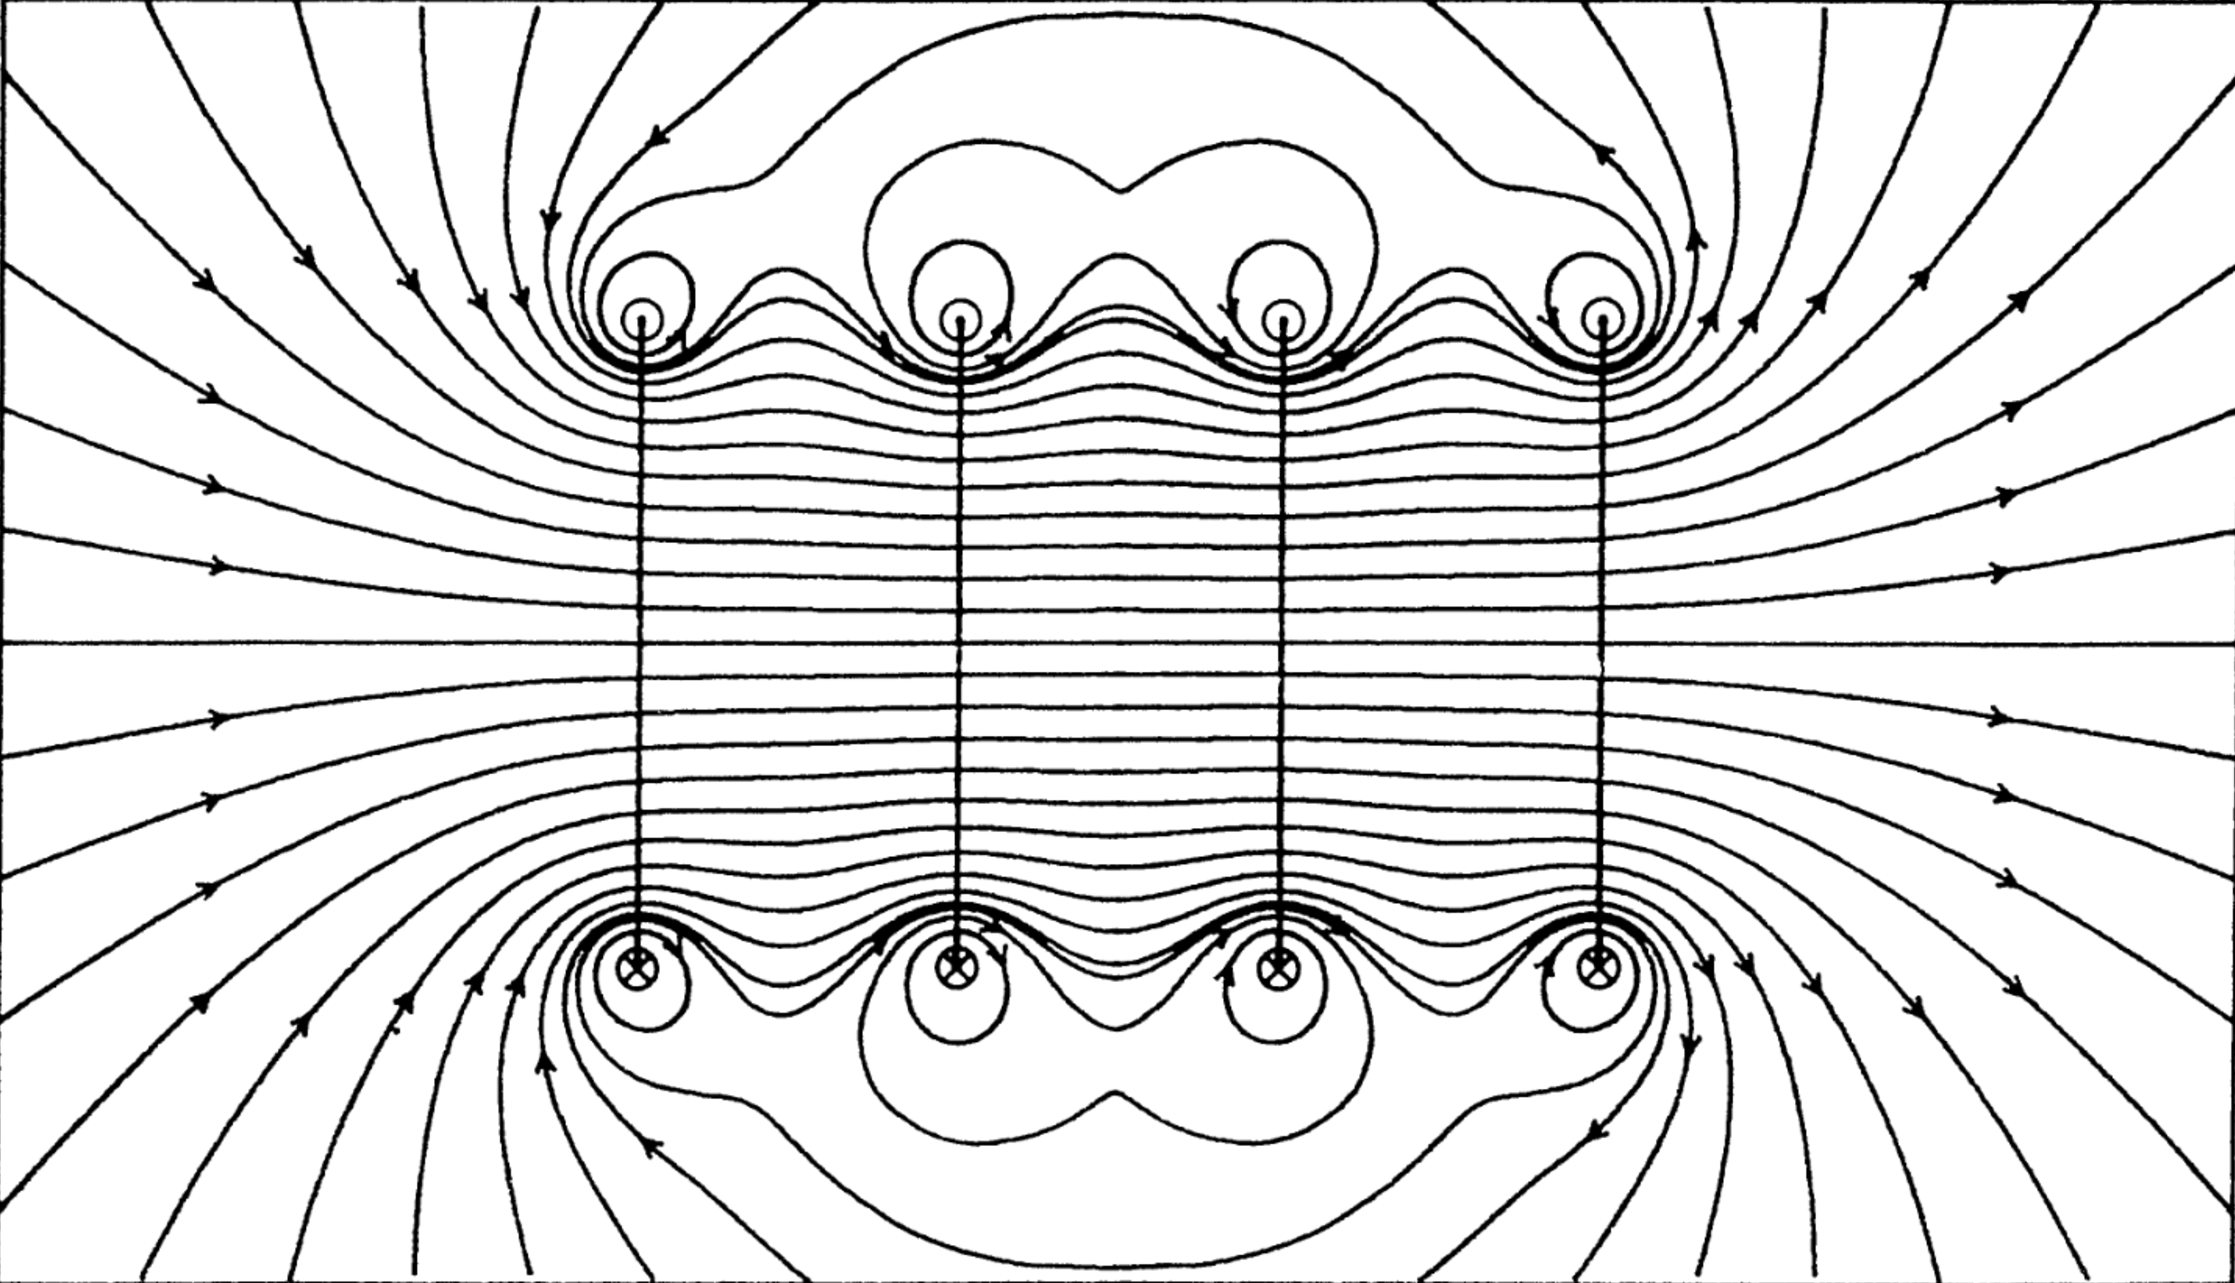
\includegraphics[width=0.7\linewidth]{solenoide}
	\caption{Lignes du champ magnétique généré par un solénoïde constitué de
		4 bobines parcourues dans le même sens par la même intensité.
		Cette figure est extraite de \cite{Gie1985}}%
	\label{fig:magneto_solenoide}
\end{figure}

\begin{enumerate}
	\item On remarque tout d'abord que les lignes de champ 
	  sont des contours fermés qui entourent les fils parcourus par un courant.
	  Cette première observation est une conséquence directe de l'équation
	  de Maxwell-Ampère. L'orientation de ces lignes de champ s'obtient
	  d'ailleurs en considérant le sens du courant dans les fils et en utilisant
	  la règle de la main droite.
      \item La divergence nulle de $\vecb$ est aussi visible sur cette carte de 
	champ. En effet, on constate que les lignes de champ ne convergent/divergent
	pas en un point de l'espace, contrairement au champ électrostatique.
      \item Dans le cas du champ magnétique, le resserrement des lignes de champ
	traduit une augmentation de la norme de ce dernier. On conclut que le champ
	est plus intense à l'intérieur du solénoïde qu'à l'extérieur. De plus, les
	lignes de champ étant parallèles à l'intérieur du solénoïde, on conclut que
	le champ est uniforme.
      \item Grâce aux lignes de champ, on retrouve rapidement les plans de 
	  symétrie et d'antisymétrie du champ magnétique. Le plan médiateur 
	  du solénoïde est par exemple un plan de symétrie du champ magnétique. 
          L'analyse de ces symétries sera utile pour calculer le champ
          magnétique résultant d'une distribution de courant.
\end{enumerate}

\section{Calcul du champ magnétostatique}
\label{sec:calcul_e}
Nous allons voir dans cette partie comment nous pouvons utiliser le théorème d'Ampère
pour calculer le champ magnétostatique $\vecb$ créé 
par une distribution de courants simple. Nous nous intéressons ici à une bobine
torique constituée d'un fil régulièrement bobiné autour d'un tore de section
carré (voir Fig.~\ref{fig:magneto_tore}). Cette bobine est caractérisée par le nombre $N$
total de spires bobinés, son rayon intérieur $R$ 
et sa hauteur $h$. La bobine est parcourue par un courant $I$.

On cherche à déterminer 
l'expression du champ électrique $\vecb$ en un point $M$ de l'espace. Pour ce faire, 
il suffit de suivre le mode d'emploi suivant
\begin{enumerate}
	\item Faire un schéma du système ! C'est absolument indispensable
	  (voir Fig.~\ref{fig:magneto_tore})
	\item Choisir un repère adapté au problème
	\item Étudier les invariances de cette distribution
	\item Étudier les symétries de la distribution de courants à l'origine 
	  du champ magnétostatique
	\item Choisir un contour d'Ampère et appliquer le théorème d'Ampère.
\end{enumerate}

Au vu de la géométrie du système, nous choisissons ici d'utiliser 
un repère cylindrique $(O, \er, \etheta, \ez)$.
Le point $M$ est donc repéré par ses coordonnées $(r, \theta, z)$. Le champ
magnétostatique en $M$ s'écrit de manière générale

\begin{equation}
	\vecb(M) = B_r(M)\er + B_\theta(M)\etheta + B_\varphi(M)\ephi.
	\label{eq:tore}
\end{equation}
Le champ magnétostatique est un vecteur à trois composantes et chaque composante
dépend des coordonnées de $M$. Pour simplifier cette expression, il est intéressant
de considérer les invariances et symétries de la distribution de courant qui génère
le champ $\vecb$.

\begin{figure}
	\centering
	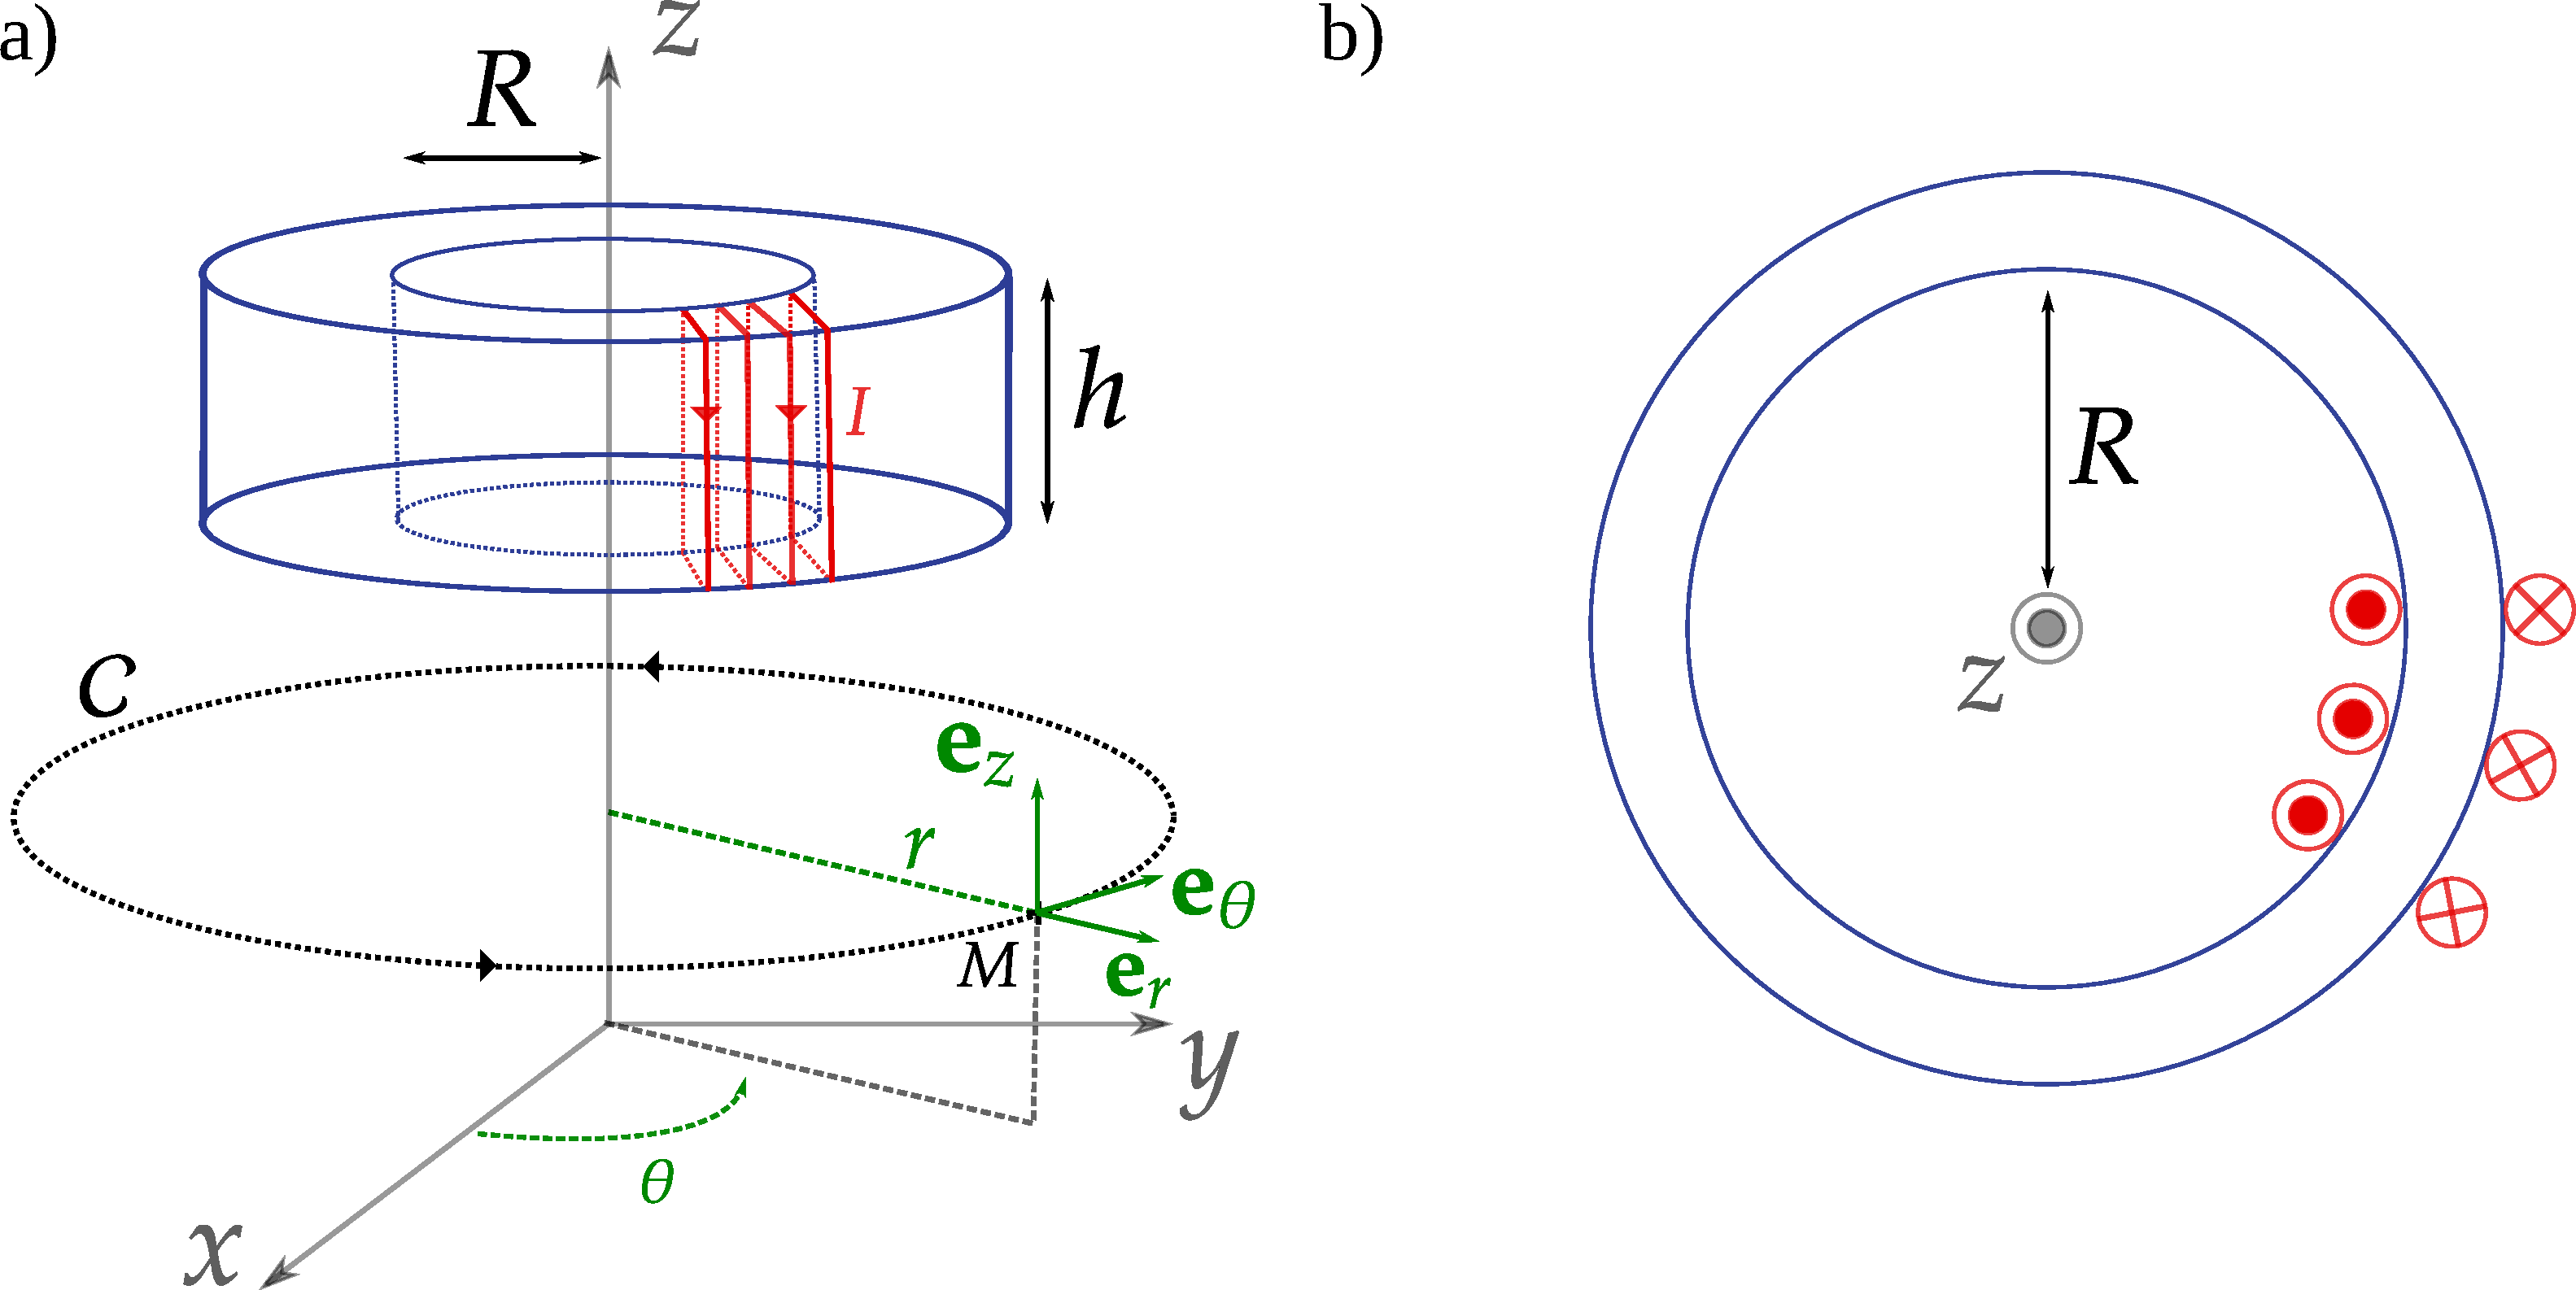
\includegraphics[scale=1]{tore}
	\caption{Bobine torique à gauche et coupe perpendiculaire à $(Oz)$
	de cette bobine à droite.}%
	\label{fig:magneto_tore}
\end{figure}

\subsection{Invariance de la distribution de courants}
On cherche ici à savoir si la distribution de courant est modifiée sous l'effet
d'une translation ou d'une rotation de l'espace. En d'autres termes, on regarde
de quelles variables elle dépend. Étant donné que les spires sont uniformément
répartie sur le tore, on observe que

\begin{itemize}
	\item  si je tourne le tore d'un angle $\Delta \theta$ dans la
	  direction $\etheta$, le problème
	  ne change pas. La distribution de courant est donc invariante 
	  par rotation selon l'angle $\theta$. $\vecb$ \textbf{ne dépend pas de
	  $\mitbf{\theta}$}.
\end{itemize}

Finalement, l'expression~\ref{eq:tore} du champ magnétique se simplifie donc en 

\begin{equation*}
	\boxed{\vecb(M) = B_r(r,z)\er + B_\theta(r,z)\etheta + B_z(r,z)\ez.}
\end{equation*}
\subsection{Symétries de la distribution de courants}

Si on applique ce principe au champ magnétique créé par une distribution 
de courants, cela revient à dire que les symétries de la distributions de 
courants doivent se retrouver dans les symétries du champ magnétique. On en 
déduit les règles suivantes

\begin{defn}[Symétries de $\vecb$ et de la distribution de courant]
\begin{itemize}
  \item si $(\Pi)$ est un plan d'antisymétrie de la distribution de courant et que 
    $M$ appartient à $(\Pi)$, alors obligatoirement $\vecb(M)$ doit 
    appartenir à $(\Pi)$,
  \item si $(\Pi)$ est un plan de symétrie de la distribution de courant 
    et que $M$ appartient à $(\Pi)$, alors obligatoirement $\vecb(M)$ doit 
    être orthogonal à $(\Pi)$.
\end{itemize}
\end{defn}

\begin{rem}
	Le champ magnétostatique $\vecb$ appartient aux plans d'\textbf{antisymétrie}
	de la distribution de courant et non aux plans de symétrie comme
	c'est le cas pour le champ électrostatique. Le vecteur $\vecb$ est 
	qualifié de vecteur axial.
\end{rem}

Pour appliquer ces règles à notre exemple, on détermine les plans de symétrie 
et d'antisymétrie de la distribution de courants auquels 
le point $M$ appartient

\begin{itemize}
	\item le plan $(M, \er, \ez)$ est un plan de symétrie de la distribution
	  de courant. $\vecb(M)$ \textbf{doit être orthogonal à ce plan}.
\end{itemize}

$\vecb(M)$ doit être orthogonal au plan $(M, \er, \ez)$, 
il doit donc être colinéaire à $\etheta$

\begin{framed}
\begin{equation*}
	\vecb(M) = B_\theta(r, z) \etheta.
\end{equation*}
\end{framed}

Nous n'avons imposé aucune condition sur la position de $M$, cette relation est
donc vraie pour tout point $M$ de l'espace. Maintenant que l'expression du 
champ magnétique a été simplifiée au maximum, on cherche à appliquer le théorème
d'Ampère.

\subsection{Application du théorème d'Ampère}
La distribution de courant présente une symétrie de révolution. On choisit comme contour 
d'Ampère un cercle $\mathcal{C}$ de rayon $r$, de centre $O$ et orienté
dans le sens de $\etheta$ qui passe par $M$ 
(voir Fig~\ref{fig:magneto_tore}) et on applique le théorème d'Ampère à ce dernier

\begin{equation*}
	\oint_\mathcal{S} \vecb(M) \cdot \dl = \mu_0 I_\mathrm{int},
	\label{eq:cavite_gauss}
\end{equation*}
où $I_\mathrm{int}$ est la courant enlacé par $\mathcal{C}$. On commence
par déterminer l'expression du membre de gauche. Dans un repère cylindrique,

\begin{equation*}
	\dl = r \dtheta \etheta.
\end{equation*}
On obtient alors
\begin{equation*}
	\oint_\mathcal{C} \vecb(M) \cdot \dl = 
	\oint_\mathcal{C} B(r,z) \etheta \cdot r \dtheta \etheta
	= B(r, z) r \int_0^{2 \pi} \dtheta
	= 2 \pi r B(r,z).
\end{equation*}
On s'intéresse maintenant au terme de droite de l'équation.
Deux cas de figure se présentent:
\begin{itemize}
	\item $M$ est situé dans le tore: le courant enlancé par $\mathcal{C}$ est alors
	  $I_\mathrm{int} = NI$.
       \item $M$ est situé à l'extérieur du tore: le courant enlacé par 
	       $\mathcal{C}$ est donc nul. Soit parce que le contour n'enlace 
	       aucun courant, soit parce qu'il enlace autant de courants positifs
	       que de courants négatifs.
\end{itemize}
Finalement,
\begin{framed}
\begin{itemize}
	\item si $M$ se trouve à l'intérieur du tore, 
	  $\vecb(M) = \dfrac{\mu_0 N I}{2 \pi r} \etheta$.
	\vspace{1em}
\item si $M$ est en dehors du tore, $\vecb(M) = \mitbf{0}$. 
\end{itemize}
\end{framed}
%\nocite{*}
%\putbib[magnetostatique]

%\newpage

%\input{exercices/magnetostatique}



\nocite{*}
\putbib[Chapitre_3/magnetostatique]
\newpage
\section{Exercices}

\begin{exocor}[Orage et boussole] 
On cherche dans cet exercice à déterminer le
champ magnétique créé par un éclair lors d'un orage.  En première
approximation, un éclair peut-être assimilé à un fil rectiligne de rayon
$a = \unit{10}{\centi \meter}$ parcouru par un courant d'intensité constante
$I = \unit{10^5}{\ampere}$.  
\begin{enumerate} 
	\item Faire un schéma modélisant un éclair. 
	Quel est le repère adapté au problème ici ?  
	\item  
	De quelle(s) variable(s) dépend l'amplitude du champ magnétique ? 
	Par quel vecteur est-il porté ?  
	Dessiner les lignes du champ magnétique produit par cet éclair.
	\item Déterminer l'expression du champ magnétique créé par l'éclair.
	      Vérifier l'homogénéité de votre expression.  
	\item L'aiguille d'une boussole peut se retrouver désaimantée 
	lorsqu'elle est placée dans un champ supérieur à 
	$B_L = \unit{2 \times 10^{-3}}{\tesla}$. À quelle distance minimale d'un
	éclair doit donc se trouver une boussole pour ne pas être désaimantée ?
\end{enumerate} 
\end{exocor}

\begin{exocor}[Bobines de Helmholtz]
Les bobines de Helmholtz sont un dispositif expérimental constitué de 
deux bobines circulaires de même rayon, parallèles et placées à une distance
égale à leur rayon. Dans cet exercice, on cherche à déterminer le champ magnétique
généré par ce système.

On considère tout d'abord une spire de rayon $R$, d'axe $Oz$, 
parcouru par un courant $I$ et
placée en $z = 0$.
On souhaite calculer le champ magnétique $\vecb_1$ créé par cette spire sur son axe,
le calcul en dehors de l'axe étant un peu plus difficile.
\begin{enumerate}
	\item Étudier les symétries et invariance de la distribution de courants.
	\item En utilisant la loi de Biot et Savart, déterminer le champ magnétique
	  généré par la spire en un point $M$ de son axe. Exprimer $B_1(M)$
	  sous la forme $B_1(M) = B_0 f(M)$ où $B_0$ est l'amplitude
	  du champ au centre de la spire et $f$ une fonction de l'espace à déterminer.
	\item Étudier la fonction $f$.
	\item On ajoute une seconde spire identique à la première en $z = R$. 
	  Déterminer le champ magnétique $\vecb$ créé par les deux spires en un point $M$ 
	  de l'axe $(Oz)$ et le mettre sous la forme $B(M) = B_0g(M)$, où 
	  $g$ est une fonction à expliciter.
  \item Tracer l'évolution de $B(M)/B_0$ avec $z/R$. 
	   Que peut-on dire de la forme des 
	   lignes de champs près de l'axe dans la zone $z = R/2$ ?
\end{enumerate}
\end{exocor}

\begin{figure}[h]
	\centering
	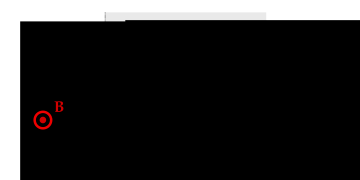
\includegraphics[scale=0.8]{supra}
	\caption{Supraconducteur occupant le demi-espace $x > 0$ baignant dans
	un champ magnétique uniforme $\vecb$ colinéaire à $\ez$.}%
	\label{fig:supra}
\end{figure}

\begin{exocor}[Effet Meissner]
	Dans un matériau supraconducteur, la densité de courant $\mathbf{j}$ 
	vérifie l'équation de London 
\begin{equation*}
	\grad \times \vecj = -\frac{\vecb}{\mu_0 \lambda^2},
\end{equation*} 

où $\mu_0$ est la perméabilité du vide, $\lambda$ une constante dépendant du 
matériau étudié et $\vecb$ le champ magnétique

On se place ici dans un repère carthésien $(0,\ex,\ey,\ez)$. 
Un supraconducteur occupe tout le demi-espace défini par $x > 0$.
À l'extérieur du supraconducteur, le champ est uniforme d'amplitude $B_0$ et 
porté par $\ez$ (voir Fig.~\ref{fig:supra}).
On admettra ici que le champ est continu à la frontière entre le vide et le 
supraconducteur et qu'il ne dépend que de $x$ à l'intérieur de ce dernier.

\begin{enumerate}
	\item Faire une analyse dimensionnelle pour déterminer la dimension de $\lambda$.
	\item Montrer qu'à l'intérieur du supraconducteur, 
	  l'évolution spatiale de l'amplitude du  champ magnétique est donnée par 
		\begin{equation*}
			\dd{^2B}{x^2} - \frac{B}{\lambda^2} = 0.
		\end{equation*}
	On utilisera l'égalité vectorielle suivante, vérifiée pour tout 
	vecteur $\vecb$,
	\begin{equation*} 
		\rot(\rot \vecb) = \gradient(\div\vecb) - \laplacien \vecb,
	\end{equation*}
	où $\laplacien$ correspond à l'opérateur laplacien vectoriel.
	\item La solution générale à cette équation différentielle est de la forme 
\begin{equation}
	B(x) = C \exp(x/\lambda) + D \exp(-x/\lambda),
\end{equation}

où $C$ et $D$ sont deux constantes réelles.
Déterminer l'expression de $C$ et $D$.

\item Pour l'aluminium, $\lambda = 16$\,nm, déterminer le rapport $B(x)/B_0$ pour $x = \lambda,\ 10\lambda,\ 100\lambda$. Proposer alors une interprétation de $\lambda$.
\end{enumerate}

L'impossibilité du champ magnétique externe à pénétrer dans le supraconducteur n'est pas anodine.
Elle induit une force de pression qui s'exerce sur le supraconducteur et peut permettre notamment de faire léviter l'aimant à l'origine de ce champ.. 
Pour en apprendre plus sur les supraconducteurs et leurs propriétés, 
vous pouvez notamment aller voir 
\href{https://www.youtube.com/watch?v=5SF98Ph8hSU}{la vidéo}
\footnote{https://www.youtube.com/watch?v=5SF98Ph8hSU} que 
le Commissariat à l'Énergie Atomique et aux Énergies Alternatives (CEA) a réalisée 
sur le sujet.
\end{exocor}

\begin{exocor}[Champ créé par un câble coaxial]
	On considère un câble coaxial (câble de sortie d'un générateur basse fréquence)
	constitué d'un cylindre métallique central plein de rayon $R_1$ et d'une 
	couche cylindrique de rayon interne $R_2$ et de rayon externe $R_3$. 
	Entre $R_1$ et $R_2$ se trouve une matière isolante assimilable à du vide d'un 
	point de vue électromagnétique. 
	
	On se place dans un repère cylindrique 
	$(O, \er, \etheta, \ez)$. Un point $M$ de l'espace es donc repérér par 
	ses coordonnées $(r, \theta, z)$. Le câble d'axe $(Oz)$ est considéré
	comme infiniment long. La partie conductrice centrale est parcourue 
	par un courant uniforme d'intensité $I$ tandis que la partie périphérique
	est parcourue par un courant uniforme d'intensité $-I$.

	\begin{enumerate}
		\item Réaliser un schéma du système.
		\item Montrer que le champ magnétique $\vecb$ au point $M$ s'écrit
		\begin{equation*}
			\vecb(M) = B(r) \vec{u},
		\end{equation*}
		où $\vec{u}$ est un vecteur à préciser.
		\item Quelle est la valeur du champ magnétique $\vecb$ au point $M$
		  si $r > R_3$ ? Quel est l'avantage d'un câble coaxial par rapport
		  à un simple fil ?
		\item Exprimer les vecteurs densités de courant $\vecj_c$ et 
		  $\vecj_p$ respectivement du conducteur central et du conducteur 
		  périphérique.
		\item Déterminer l'expression du champ magnétique $\vecb$ pour
		  un point $M$ à l'intérieur du câble.
	\end{enumerate}
\end{exocor}
\newpage
\section{Corrigé}
\begin{corrige}
\begin{enumerate}
\item Voir figure~\ref{fig:magneto_spire}. On se place donc dans un repère cylindrique
      $(O, \er, \etheta, \ez)$. Un point $M$ est repéré par ses coordonnées 
      $(r, \theta, \phi)$.

\item  L'étude
      des invariances de la distribution de courant montre que la norme du 
      champ magnétique \fbox{ne dépend que de la distance au fil $r$}. L'étude des
      symétries montre que le champ magnétique est \fbox{orthoradial}.
      Les lignes de champ sont des \fbox{cercles concentriques} centrés le fil.

\item Voir cours. L'expression du champ magnétique en un point $M$ situé 
  à une distance $r$ du fil est donnée par
  \begin{equation*}
	  \vecb(M) = \dfrac{\mu_0 I}{2 \pi R} \etheta.
   \end{equation*}
   On vérifie la dimension de cette expression. D'après le théorème d'Ampère
   on sait que la circulation de $\vecb$ sur un contour fermé est égale à 
   $\mu_0 I$. Or la circulation de $\vecb$ est homogène à champ magnétique 
   multiplié par une longueur ($\vecb \cdot \dl$). L'expression est donc bien homogène.

   \item 
	   \begin{equation*}
		B(M) < B_L \iff \dfrac{\mu_0 I}{2 \pi r} < B_L \iff 
		r > \dfrac{\mu_0 I}{2 \pi B_L} \iff \boxed{r > \unit{10}{\meter}} 
	   \end{equation*}
	Si la boussole se trouve à moins de $\unit{10}{\meter}$ de l'éclair, 
	elle sera désaimantée.
\end{enumerate}
\end{corrige}

\begin{corrige} 
	\begin{enumerate}
		\item On commence bien sûr par réaliser un schéma du système
			(voir Fig.~\ref{fig:spire_ex}).
		      On choisit d'utiliser dans cet exercice un repère cylindrique
		      $(O, \er, \etheta, \ez)$. Un point $M$ de l'axe $(Oz)$
		      est donc repéré par ses coordonnées $(0, 0, z)$. Sous
		      sa forme la plus générale, le champ magnétique en $M$ 
		      s'écrit 
		      \begin{equation*}
			      \vecb_1(M) = B_r(M) \er + B_\theta(M) \etheta +
			      B_z(M) \ez.
		      \end{equation*}

		      \begin{description}
			     \item[Invariance:] La distribution de courant est 
			     invariante par rotation autour de l'axe $(Oz)$, 
			     $B_1$ ne dépend donc pas de $\theta$. De plus, on 
			     s'intéresse à un point $M$ situé sur l'axe, la
			     distance $r$ à l'axe de la spire n'entre donc pas
			     en compte dans le problème.
		     \item[Symétrie: ] Tout plan contenant l'axe $(Oz)$ est 
			               plan d'antisymétrie de la distribution de courant,
				       $\vecb_1(M)$ doit donc appartenir à l'intersection
				       de tous ces plans. $\vecb_1(M)$ est donc colinéaire
				       à $\ez$.
		     \end{description}
		     Finalement,
		     \begin{equation*}
			     \boxed{\vecb_1(M) = B_z(z) \ez.}
		     \end{equation*}
		
		\item La première étape est de déterminer le champ magnétique généré
		  par une portion $\dl_P$ de la spire centrée au point $P$
		  de coordonnées $(R, \theta, 0)$.On commence donc par exprimer $\dl_P$ 
		  dans le système de coordonnées choisi
		  \begin{equation*}
			  \dl_P = R \dtheta \etheta.
		  \end{equation*}
		  Vient ensuite l'expression de $\mitbf{PM}$ 
		  dans ce même référentiel
		  \begin{equation*}
			  \mitbf{PM} = \mitbf{PO} + \mitbf{OM} = -R \er + z\ez.
		  \end{equation*}
		  On aboutit ainsi à l'expression du champ magnétique $
		  \mathrm{\textbf{d}}\vecb_P(M)$
		  généré par cette portion de spire en $M$
		  \begin{equation*}
			  \mathrm{\textbf{d}}\vecb_P(M) = \dfrac{\mu_0 I}{4 \pi} \times 
			  \dfrac{\dl_P \wedge \mitbf{PM}}{PM^3}
			  = \dfrac{\mu_0 I}{4 \pi} \times \dfrac{R^2\ez + Rz\er}
			  {\left(R^2 + z^2\right)^{3/2}} \dtheta.
		  \end{equation*}
		  Il ne reste finalement plus qu'à sommer les contributions 
		  de toutes les portions de la spire pour aboutir au champ total
		  $\vecb_1(M)$
		  \begin{equation*}
			  \vecb_1(M) = \int_0^{2\pi} \dfrac{\mu_0 I}{4 \pi} \times 
			  \dfrac{R^2\ez + Rz\er}
			  {\left(R^2 + z^2\right)^{3/2}} \dtheta
			  = \dfrac{\mu_0 I}{4 \pi\left(R^2 + z^2\right)^{3/2}} 
			  \left(
		            R^2\ez  
		    \int_0^{2\pi}\dtheta + Rz \int_0^{2\pi} \er \dtheta
		     \right)
		     = \dfrac{\mu_0 I R^2}{2 \left(R^2 + z^2\right)^{3/2}}\ez.
		  \end{equation*}
		  $B_0$ est le champ obtenu en $z = 0$, il vaut donc
		  \begin{equation*}
			  B_0 = \dfrac{\mu_0 I}{2 R}.
		  \end{equation*}
		  On obtient finalement
		  \begin{equation*}
			  \boxed{\vecb_1(M) = B_0 \times 
			  \left[1 + \left(\dfrac{z}{R}\right)^2\right]^{-3/2}\ez.}
		  \end{equation*}
		  La figure~\ref{fig:helmholtz} représente l'évolution de 
		  $B(M)/B_0$ avec $z/R$.
		  \begin{figure}[htpb]
		  	\centering
			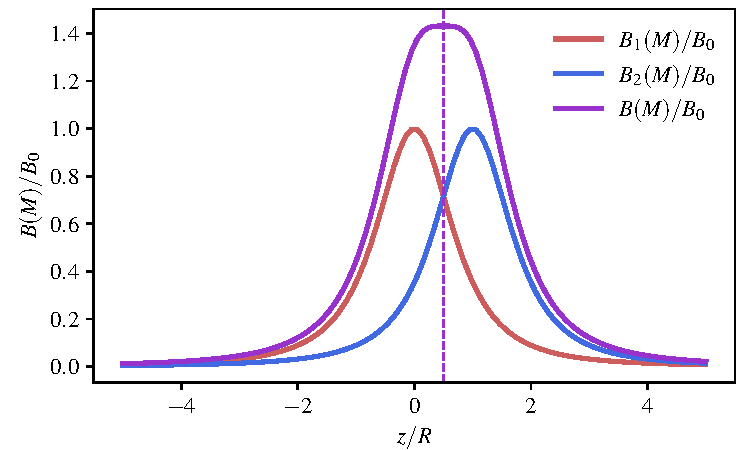
\includegraphics[scale=0.8]{helmholtz}
			\caption{$B_1(M)/B_0$, $B_2(M)/B_0$ et $B(M)/B_0$ 
			         en fonction de $z/R$. La ligne en pointillé correspond
			 à l'abscisse $z/R = 1/2$.}%
			\label{fig:helmholtz}
		  \end{figure}

	  \item On ajoute ensuite une seconde spire qui génère en $M$ un champ magnétique
		$\vecb_2(M)$. La spire $2$ étant identique à la première, on écrit
		directement que
		\begin{equation*}
			\vecb_2(M) = B_0 \times \left[1 + \left(\dfrac{z - R}{R}\right)^2
			\right]^{-3/2}\ez.
		\end{equation*}
		En utilisant le principe de superposition, on en déduit le champ
		magnétique total $\vecb$ généré en $M$
		\begin{equation*}
			\boxed{\vecb(M) = \vecb_1(M) + \vecb_2(M) 
			         = B_0 \left\{\left[1 + \left(\dfrac{z}{R}\right)^2
				 \right]^{-3/2} + \left[1 + \left(\dfrac{z-R}{R}\right)^2
	 \right]^{-3/2}\right\} \ez.}
		\end{equation*} 
		La figure~\ref{fig:helmholtz} trace l'évolution de $B(M)/B_0$ 
		en fonction de $z/R$. On remarque sur cette figure que la fonction est
		constante autour de $R/2$. Les lignes de champ seront donc \fbox{parallèles}
		autour de ce point.

	\end{enumerate}

\end{corrige}
\begin{figure}[htpb]
	\centering
	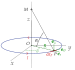
\includegraphics[scale=0.75]{spire}
	\caption{Schéma de la spire.}%
	\label{fig:spire_ex}
\end{figure}
\begin{corrige}
\begin{enumerate}
	\item On sait d'après l'équation de Maxwell-Ampère que 
	\begin{equation*}
		\rot \vecb = \mu_0 \vecj.
	\end{equation*}
	$\mu_0 \rot \vecj$ est donc homogène à un champ magnétique divisé par le carré
	d'une longueur. \fbox{$\lambda$ est donc homogène à une longueur.}

	\item D'après l'équation de Maxwell-Ampère, on a
	\begin{equation*}
		\rot \vecb = \mu_0 \vecj \Rightarrow \rot(\rot \vecb) = \mu_0 \rot \vecj.
	\end{equation*}
	En utilisant l'équation de London et l'égalité vectoriel fournie cela donne
	\begin{equation*}
		\rot(\rot \vecb) = -\dfrac{\vecb}{\lambda^2} \iff
		\gradient(\div \vecb) - \laplacien(\vecb) = -\dfrac{\vecb}{\lambda^2}.
	\end{equation*}
	En utilisant l'équation de Maxwell-Thomson, $\div \vecb = 0$, on aboutit ainsi à
	\begin{equation*}
		\boxed{\dd{^2B}{x^2} - \dfrac{B}{\lambda^2} = 0.}
	\end{equation*}

	\item $C$ doit obligatoirement être nul. Dans le cas contraire l'amplitude du
	      champ magnétique divergerait lorsque $x$ tend vers $\infty$. Pour déterminer $D$,
	      on utilise la continuité du champ en $x = 0$. On a donc directement
	      \begin{equation*}
		      \boxed{\vecb(x) = B_0 \exp\left(\dfrac{-x}{\lambda}\right)\ez.}
	      \end{equation*}
	
	\item
	\begin{equation*}
	     \begin{array}{c|lll}
			x	& \lambda & 10\lambda & 100\lambda \\[0.3em] \hline \\[0.2em]
			B(x)/B_0 & 0.37    & 4.5 \times 10^{-5} & 3.7 \times 10^{-44} \\[1em]
	      \end{array}
	\end{equation*}

	     $\lambda$ correspond donc à la profondeur de pénétration de $\vecb$
	     dans le supraconducteur.
\end{enumerate}
\end{corrige}

\begin{corrige}
\begin{enumerate}
	\item Le système est représenté sur la figure~\ref{fig:magneto_coaxial}.
		\begin{figure}[h]
		\centering
		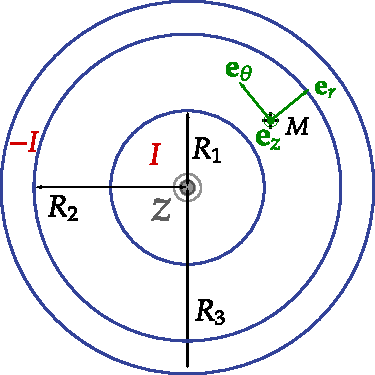
\includegraphics[scale=0.8]{coaxial}
		\caption{Coupe du câble coaxial dans le plan $(O, \er, \etheta)$.}
		\label{fig:magneto_coaxial}
	\end{figure}
	\item Sous sa forme la plus générale, le champ magnétique en $M$ 
	      s'écrit 
		      \begin{equation*}
			      \vecb(M) = B_r(M) \er + B_\theta(M) \etheta +
			      B_z(M) \ez.
		      \end{equation*}

		      \begin{description}
			     \item[Invariance:] La distribution de courant est 
			     invariante
			     \begin{itemize}
			     	\item par rotation autour de l'axe $(Oz)$, 
			     	      $\vecb$ ne dépend donc pas de $\theta$.
				\item par translation selon l'axe $(Oz)$, $\vecb$
				      ne dépend donc pas de $z$.
			     \end{itemize}
			      \item[Symétrie: ]
			      Le plan $(M, \er, \ez)$ est plan 
			      de symétrie de la distribution de 
			      courants. $\vecb(M)$ est donc 
			      orthogonal à ce plan et est donc colinéaire à
			      $\etheta$.
		      \end{description}
		     Finalement,
		     \begin{equation*}
			     \boxed{\vecb(M) = B(r) \etheta.}
		     \end{equation*}
	
	  \item Si $r > R_3$, le point $M$ se trouve à l'extérieur du câble 
		coaxial. Si on applique le théorème d'Ampère à un cercle 
		$\mathcal{C}$ de rayon $r$ et de centre $O$, cela donne
		\begin{equation*}
			\oint_\mathcal{C} \vecb \cdot \dl = \mu_0(I - I) = 0.
		\end{equation*}
		Ici, on $\dl = r \dtheta \etheta$ donc on obtient directement 
		\begin{equation*}
			\boxed{B(r) = 0}.
		\end{equation*}
		\fbox{Le champ magnétique est donc nul en dehors du câble.} Un câble 
		coaxial permet donc d'éviter de générer un champ magnétique parasite.

	\item   Les vecteurs densité de courant $\vecj_c$ et $\vecj_p$ sont réliés 
		à l'intensité $I$ du courant par les relations
		\begin{equation*}
			I = \iint_{S_c} \vecj_c \cdot \ds
			\quad \mathrm{et} \quad
			-I = \iint_{S_p} \vecj_p \cdot \ds,
		\end{equation*}
		où $S_c$ et $S_p$ sont respectivement les sections de la partie centrale
		et de la partie périphériques.
		Dans la partie centrale comme dans la partie périphérique, le
	        courant est uniforme. Les vecteurs densités de courant s'expriment
		donc
		\begin{equation*}
			\boxed{
			\vecj_c = \dfrac{I}{\pi R_1^2} \ez
			\quad \mathrm{et} \quad 
			\vecj_p = \dfrac{-I}{\pi \left(R_3^2 - R_2^2 \right)}
			\ez.
		}
		\end{equation*}

	\item On peut alors appliquer le théorème d'Ampère à un cercle $\mathcal{C}$
	      de rayon $r$ et de centre $O$
	      \begin{equation*}
		      \oint_\mathcal{C} \vecb \cdot \dl = I_\mathrm{enlacé},
	      \end{equation*}
	      où $I_\mathrm{enlacé}$ est le courant enlacé par $\mathcal{C}$.

	      On commence alors par exprimer le terme de gauche. On a $\dl = 
	      r \dtheta \etheta$ et donc le terme de gauche vaut $2 \pi r B(r)$.
	      Pour le terme de droite, c'est un peu plus compliqué. En effet, 3 cas
	      de figure se présentent

	      \begin{itemize}
		      \item Si $0 \le r \le R_1$, 
			    $I_\mathrm{enlacé} = \pi r^2 j_c = 
			    I\left(\dfrac{r}{R_1} \right)^2$.
		      \item Si $R_1 \le r \le R_2$, $I_\mathrm{enlacé} = I$.
		      \item Si $R_2 \le r \le R_3$, 
			    $I_\mathrm{enlacé} = 
			    I + \pi \left(R_3^2 - r^2\right) j_p =
			    I \left(1 - \dfrac{r^2 - R_2^2}{R_3^2 - R_2^2} \right)$.
	      \end{itemize}

	      Finalement, on obtient l'expression du champ magnétique en tout 
	      point $M$ de l'espace
	      \begin{equation*}
	      \boxed{
		     \vecb(M) = 
	      \left\{
		      \begin{array}{l}
			      \mathbf{0} \quad \mathrm{si} \quad r > R_3 \\[1em]
			      \dfrac{\mu_0 I}{2 \pi r} \left(1 - \dfrac{r^2 - R_2^2}
			      {R_3^2 - R_2^2} \right) \etheta \quad \mathrm{si} \quad
			      R_2 \le r \le R_3\\[1.5em]
			      \dfrac{\mu_0 I}{2 \pi r} \etheta \quad \mathrm{si} 
			      \quad R_1 \le r \le R_2\\[1em]
			      \dfrac{\mu_0 I}{2 \pi r}\left(\dfrac{r}{R_1}\right)^2
			      \etheta \quad \mathrm{si} \quad 0 \le r \le R_1.
		      \end{array}
		      \right.
	      }
	      \end{equation*}
\end{enumerate}
\end{corrige}

\begin{corr}{Magnétostatique}
\correction{Orage et boussole}
\begin{corrlist}
\item Voir figure~\ref{fig:magneto_spire}. On se place donc dans un repère cylindrique
      $(O, \er, \etheta, \ez)$. Un point $M$ est repéré par ses coordonnées 
      $(r, \theta, \phi)$.

\item  L'étude
      des invariances de la distribution de courant montre que la norme du 
      champ magnétique \fbox{ne dépend que de la distance au fil $r$}. L'étude des
      symétries montre que le champ magnétique est \fbox{orthoradial}.
      Les lignes de champ sont des \fbox{cercles concentriques} centrés le fil.

\item Voir cours. L'expression du champ magnétique en un point $M$ situé 
  à une distance $r$ du fil est donnée par
  \begin{equation*}
	  \vecb(M) = \dfrac{\mu_0 I}{2 \pi R} \etheta.
   \end{equation*}
   On vérifie la dimension de cette expression. D'après le théorème d'Ampère
   on sait que la circulation de $\vecb$ sur un contour fermé est égale à 
   $\mu_0 I$. Or la circulation de $\vecb$ est homogène à champ magnétique 
   multiplié par une longueur ($\vecb \cdot \dl$). L'expression est donc bien homogène.

   \item 
	   \begin{equation*}
		B(M) < B_L \iff \dfrac{\mu_0 I}{2 \pi r} < B_L \iff 
		r > \dfrac{\mu_0 I}{2 \pi B_L} \iff \boxed{r > \unit{10}{\meter}} 
	   \end{equation*}
	Si la boussole se trouve à moins de $\unit{10}{\meter}$ de l'éclair, 
	elle sera désaimantée.
\end{corrlist}


\correction{Bobines de Helmholtz}
	\begin{corrlist}
		\item On commence bien sûr par réaliser un schéma du système
			(voir Fig.~\ref{fig:spire_ex}).
		      On choisit d'utiliser dans cet exercice un repère cylindrique
		      $(O, \er, \etheta, \ez)$. Un point $M$ de l'axe $(Oz)$
		      est donc repéré par ses coordonnées $(0, 0, z)$. Sous
		      sa forme la plus générale, le champ magnétique en $M$ 
		      s'écrit 
		      \begin{equation*}
			      \vecb_1(M) = B_r(M) \er + B_\theta(M) \etheta +
			      B_z(M) \ez.
		      \end{equation*}

		      \begin{description}
			     \item[Invariance:] La distribution de courant est 
			     invariante par rotation autour de l'axe $(Oz)$, 
			     $B_1$ ne dépend donc pas de $\theta$. De plus, on 
			     s'intéresse à un point $M$ situé sur l'axe, la
			     distance $r$ à l'axe de la spire n'entre donc pas
			     en compte dans le problème.
		     \item[Symétrie: ] Tout plan contenant l'axe $(Oz)$ est 
			               plan d'antisymétrie de la distribution de courant,
				       $\vecb_1(M)$ doit donc appartenir à l'intersection
				       de tous ces plans. $\vecb_1(M)$ est donc colinéaire
				       à $\ez$.
		     \end{description}
		     Finalement,
		     \begin{equation*}
			     \boxed{\vecb_1(M) = B_z(z) \ez.}
		     \end{equation*}
		
		\item La première étape est de déterminer le champ magnétique généré
		  par une portion $\dl_P$ de la spire centrée au point $P$
		  de coordonnées $(R, \theta, 0)$.On commence donc par exprimer $\dl_P$ 
		  dans le système de coordonnées choisi
		  \begin{equation*}
			  \dl_P = R \dtheta \etheta.
		  \end{equation*}
		  Vient ensuite l'expression de $\mitbf{PM}$ 
		  dans ce même référentiel
		  \begin{equation*}
			  \mitbf{PM} = \mitbf{PO} + \mitbf{OM} = -R \er + z\ez.
		  \end{equation*}
		  On aboutit ainsi à l'expression du champ magnétique $
		  \mathrm{\textbf{d}}\vecb_P(M)$
		  généré par cette portion de spire en $M$
		  \begin{equation*}
			  \mathrm{\textbf{d}}\vecb_P(M) = \dfrac{\mu_0 I}{4 \pi} \times 
			  \dfrac{\dl_P \wedge \mitbf{PM}}{PM^3}
			  = \dfrac{\mu_0 I}{4 \pi} \times \dfrac{R^2\ez + Rz\er}
			  {\left(R^2 + z^2\right)^{3/2}} \dtheta.
		  \end{equation*}
		  Il ne reste finalement plus qu'à sommer les contributions 
		  de toutes les portions de la spire pour aboutir au champ total
		  $\vecb_1(M)$
		  \begin{equation*}
			  \vecb_1(M) = \int_0^{2\pi} \dfrac{\mu_0 I}{4 \pi} \times 
			  \dfrac{R^2\ez + Rz\er}
			  {\left(R^2 + z^2\right)^{3/2}} \dtheta
			  = \dfrac{\mu_0 I}{4 \pi\left(R^2 + z^2\right)^{3/2}} 
			  \left(
		            R^2\ez  
		    \int_0^{2\pi}\dtheta + Rz \int_0^{2\pi} \er \dtheta
		     \right)
		     = \dfrac{\mu_0 I R^2}{2 \left(R^2 + z^2\right)^{3/2}}\ez.
		  \end{equation*}
		  $B_0$ est le champ obtenu en $z = 0$, il vaut donc
		  \begin{equation*}
			  B_0 = \dfrac{\mu_0 I}{2 R}.
		  \end{equation*}
		  On obtient finalement
		  \begin{equation*}
			  \boxed{\vecb_1(M) = B_0 \times 
			  \left[1 + \left(\dfrac{z}{R}\right)^2\right]^{-3/2}\ez.}
		  \end{equation*}
		  La figure~\ref{fig:helmholtz} représente l'évolution de 
		  $B(M)/B_0$ avec $z/R$.
		  \begin{figure}[htpb]
		  	\centering
			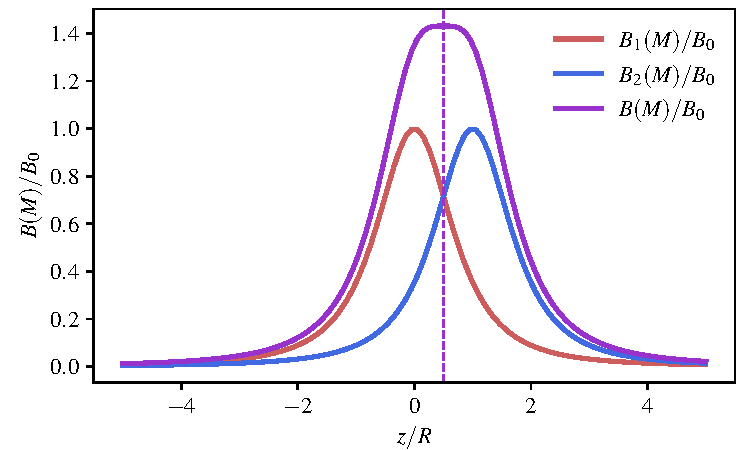
\includegraphics[scale=0.8]{helmholtz}
			\caption{$B_1(M)/B_0$, $B_2(M)/B_0$ et $B(M)/B_0$ 
			         en fonction de $z/R$. La ligne en pointillé correspond
			 à l'abscisse $z/R = 1/2$.}%
			\label{fig:helmholtz}
		  \end{figure}

	  \item On ajoute ensuite une seconde spire qui génère en $M$ un champ magnétique
		$\vecb_2(M)$. La spire $2$ étant identique à la première, on écrit
		directement que
		\begin{equation*}
			\vecb_2(M) = B_0 \times \left[1 + \left(\dfrac{z - R}{R}\right)^2
			\right]^{-3/2}\ez.
		\end{equation*}
		En utilisant le principe de superposition, on en déduit le champ
		magnétique total $\vecb$ généré en $M$
		\begin{equation*}
			\boxed{\vecb(M) = \vecb_1(M) + \vecb_2(M) 
			         = B_0 \left\{\left[1 + \left(\dfrac{z}{R}\right)^2
				 \right]^{-3/2} + \left[1 + \left(\dfrac{z-R}{R}\right)^2
	 \right]^{-3/2}\right\} \ez.}
		\end{equation*} 
		La figure~\ref{fig:helmholtz} trace l'évolution de $B(M)/B_0$ 
		en fonction de $z/R$. On remarque sur cette figure que la fonction est
		constante autour de $R/2$. Les lignes de champ seront donc \fbox{parallèles}
		autour de ce point.

	\end{corrlist}


\begin{figure}[htpb]
	\centering
	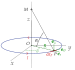
\includegraphics[scale=0.75]{spire}
	\caption{Schéma de la spire.}%
	\label{fig:spire_ex}
\end{figure}
\correction{Effet Meissner}
\begin{corrlist}
	\item On sait d'après l'équation de Maxwell-Ampère que 
	\begin{equation*}
		\rot \vecb = \mu_0 \vecj.
	\end{equation*}
	$\mu_0 \rot \vecj$ est donc homogène à un champ magnétique divisé par le carré
	d'une longueur. \fbox{$\lambda$ est donc homogène à une longueur.}

	\item D'après l'équation de Maxwell-Ampère, on a
	\begin{equation*}
		\rot \vecb = \mu_0 \vecj \Rightarrow \rot(\rot \vecb) = \mu_0 \rot \vecj.
	\end{equation*}
	En utilisant l'équation de London et l'égalité vectoriel fournie cela donne
	\begin{equation*}
		\rot(\rot \vecb) = -\dfrac{\vecb}{\lambda^2} \iff
		\gradient(\div \vecb) - \laplacien(\vecb) = -\dfrac{\vecb}{\lambda^2}.
	\end{equation*}
	En utilisant l'équation de Maxwell-Thomson, $\div \vecb = 0$, on aboutit ainsi à
	\begin{equation*}
		\boxed{\dd{^2B}{x^2} - \dfrac{B}{\lambda^2} = 0.}
	\end{equation*}

	\item $C$ doit obligatoirement être nul. Dans le cas contraire l'amplitude du
	      champ magnétique divergerait lorsque $x$ tend vers $\infty$. Pour déterminer $D$,
	      on utilise la continuité du champ en $x = 0$. On a donc directement
	      \begin{equation*}
		      \boxed{\vecb(x) = B_0 \exp\left(\dfrac{-x}{\lambda}\right)\ez.}
	      \end{equation*}
	
	\item
	\begin{equation*}
	     \begin{array}{c|lll}
			x	& \lambda & 10\lambda & 100\lambda \\[0.3em] \hline \\[0.2em]
			B(x)/B_0 & 0.37    & 4.5 \times 10^{-5} & 3.7 \times 10^{-44} \\[1em]
	      \end{array}
	\end{equation*}

	     $\lambda$ correspond donc à la profondeur de pénétration de $\vecb$
	     dans le supraconducteur.
\end{corrlist}


\correction{Champ créé par un câble coaxial}
\begin{corrlist}
	\item Le système est représenté sur la figure~\ref{fig:magneto_coaxial}.
		\begin{figure}[h]
		\centering
		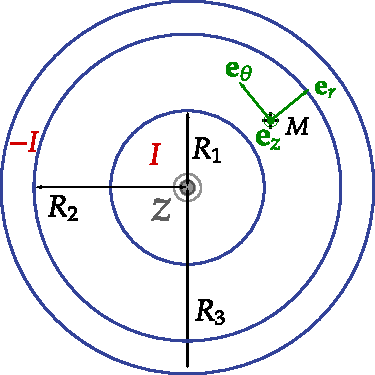
\includegraphics[scale=0.8]{coaxial}
		\caption{Coupe du câble coaxial dans le plan $(O, \er, \etheta)$.}
		\label{fig:magneto_coaxial}
	\end{figure}
	\item Sous sa forme la plus générale, le champ magnétique en $M$ 
	      s'écrit 
		      \begin{equation*}
			      \vecb(M) = B_r(M) \er + B_\theta(M) \etheta +
			      B_z(M) \ez.
		      \end{equation*}

		      \begin{description}
			     \item[Invariance:] La distribution de courant est 
			     invariante
			     \begin{itemize}
			     	\item par rotation autour de l'axe $(Oz)$, 
			     	      $\vecb$ ne dépend donc pas de $\theta$.
				\item par translation selon l'axe $(Oz)$, $\vecb$
				      ne dépend donc pas de $z$.
			     \end{itemize}
			      \item[Symétrie: ]
			      Le plan $(M, \er, \ez)$ est plan 
			      de symétrie de la distribution de 
			      courants. $\vecb(M)$ est donc 
			      orthogonal à ce plan et est donc colinéaire à
			      $\etheta$.
		      \end{description}
		     Finalement,
		     \begin{equation*}
			     \boxed{\vecb(M) = B(r) \etheta.}
		     \end{equation*}
	
	  \item Si $r > R_3$, le point $M$ se trouve à l'extérieur du câble 
		coaxial. Si on applique le théorème d'Ampère à un cercle 
		$\mathcal{C}$ de rayon $r$ et de centre $O$, cela donne
		\begin{equation*}
			\oint_\mathcal{C} \vecb \cdot \dl = \mu_0(I - I) = 0.
		\end{equation*}
		Ici, on $\dl = r \dtheta \etheta$ donc on obtient directement 
		\begin{equation*}
			\boxed{B(r) = 0}.
		\end{equation*}
		\fbox{Le champ magnétique est donc nul en dehors du câble.} Un câble 
		coaxial permet donc d'éviter de générer un champ magnétique parasite.

	\item   Les vecteurs densité de courant $\vecj_c$ et $\vecj_p$ sont réliés 
		à l'intensité $I$ du courant par les relations
		\begin{equation*}
			I = \iint_{S_c} \vecj_c \cdot \ds
			\quad \mathrm{et} \quad
			-I = \iint_{S_p} \vecj_p \cdot \ds,
		\end{equation*}
		où $S_c$ et $S_p$ sont respectivement les sections de la partie centrale
		et de la partie périphériques.
		Dans la partie centrale comme dans la partie périphérique, le
	        courant est uniforme. Les vecteurs densités de courant s'expriment
		donc
		\begin{equation*}
			\boxed{
			\vecj_c = \dfrac{I}{\pi R_1^2} \ez
			\quad \mathrm{et} \quad 
			\vecj_p = \dfrac{-I}{\pi \left(R_3^2 - R_2^2 \right)}
			\ez.
		}
		\end{equation*}

	\item On peut alors appliquer le théorème d'Ampère à un cercle $\mathcal{C}$
	      de rayon $r$ et de centre $O$
	      \begin{equation*}
		      \oint_\mathcal{C} \vecb \cdot \dl = I_\mathrm{enlacé},
	      \end{equation*}
	      où $I_\mathrm{enlacé}$ est le courant enlacé par $\mathcal{C}$.

	      On commence alors par exprimer le terme de gauche. On a $\dl = 
	      r \dtheta \etheta$ et donc le terme de gauche vaut $2 \pi r B(r)$.
	      Pour le terme de droite, c'est un peu plus compliqué. En effet, 3 cas
	      de figure se présentent

	      \begin{itemize}
		      \item Si $0 \le r \le R_1$, 
			    $I_\mathrm{enlacé} = \pi r^2 j_c = 
			    I\left(\dfrac{r}{R_1} \right)^2$.
		      \item Si $R_1 \le r \le R_2$, $I_\mathrm{enlacé} = I$.
		      \item Si $R_2 \le r \le R_3$, 
			    $I_\mathrm{enlacé} = 
			    I + \pi \left(R_3^2 - r^2\right) j_p =
			    I \left(1 - \dfrac{r^2 - R_2^2}{R_3^2 - R_2^2} \right)$.
	      \end{itemize}

	      Finalement, on obtient l'expression du champ magnétique en tout 
	      point $M$ de l'espace
	      \begin{equation*}
	      \boxed{
		     \vecb(M) = 
	      \left\{
		      \begin{array}{l}
			      \mathbf{0} \quad \mathrm{si} \quad r > R_3 \\[1em]
			      \dfrac{\mu_0 I}{2 \pi r} \left(1 - \dfrac{r^2 - R_2^2}
			      {R_3^2 - R_2^2} \right) \etheta \quad \mathrm{si} \quad
			      R_2 \le r \le R_3\\[1.5em]
			      \dfrac{\mu_0 I}{2 \pi r} \etheta \quad \mathrm{si} 
			      \quad R_1 \le r \le R_2\\[1em]
			      \dfrac{\mu_0 I}{2 \pi r}\left(\dfrac{r}{R_1}\right)^2
			      \etheta \quad \mathrm{si} \quad 0 \le r \le R_1.
		      \end{array}
		      \right.
	      }
	      \end{equation*}
\end{corrlist}
\end{corr}

\end{bibunit}

\begin{bibunit}
\graphicspath{{Chapitre_4/figure/}}
\chapter{Étude macroscopique de l'aimantation}
\begin{objectif}
	\item Connaître la notion de dipôle magnétique
	\item Connaître les différents types de magnétisme et la notion
	  d'aimantation induite
	\item Connaître les équations qui contrôlent l'évolution spatiale
	  du champ magnétique dans les milieux magnétiques
	\item Savoir décrire un cycle d'hystérésis et donner une explication
          microscopique à ce dernier
\end{objectif}
\section*{Introduction}
Dans ce chapitre, nous allons étudier les propriétés magnétiques des matériaux 
en les abordant d'un point de vue macroscopique. Quelques rares matériaux 
sont capables de générér leur propre champ magnétique (les aimants par exemple).
On dit alors qu'ils possèdent une \textbf{aimantation permanente}.
La plupart du temps leurs propriétés magnétiques
ne se manifestent que sous l'action d'un champ magnétique produit par une autre source
(une boussole par exemple). Ils se mettent alors à produire un champ propre qui
perturbe le champ dans lequel ils baignent initialement. 
On dit que ces matériaux possèdent une \textbf{aimantation
induite}.
\section{Le dipôle magnétique}
	Lorsqu'un observateur se trouve loin d'un circuit filiforme, il devient insensible
	aux caractéristiques géométriques de ce dernier. Le champ magnétique perçu par ce 
	dernier ne dépendra plus de la taille de la spire ou de sa forme. La spire 
	pourra alors être considéré comme un \textbf{dipôle magnétique}.

	\begin{defn}{Dipôle magnétique}
		Un dipôle magnétique est une source de champ magnétique (aimant 
		ou circuit parcouru par un courant $I$) de dimension typique $a$
		vu de loin, c'est-à-dire depuis une distance $r \gg a$.
	\end{defn}

	\begin{rema}
		De la même manière, deux particules portant une charge opposée
		peuvent être assimilées à grande distance à un dipôle électrique.
	\end{rema}
	
	Nous allons voir que ce modèle est très utile lorsqu'il s'agit de décrire
	le comportement magnétique de la matière. 
	
	\subsection{Champ magnétique d'une spire}
	Pour illustrer le notion de dipôle magnétique,
	nous considérons maintenant une spire de rayon $a$ parcourue par un courant $I$
	(voir Fig.~\ref{fig:aimant_spire}).
	L'idée est de calculer une approximation du champ généré par cette spire
	à une distance $r \gg a$. On considère un point $M$ situé dans le plan 
	$(O, \ey, \ez)$ et reperé par ses coordonnées polaire $(r, \theta)$, 
	où $\theta$ est l'angle entre $\ey$ et $\er$.

	\begin{figure}[htpb]
		\centering
		\includegraphics[]{aimant_spire}
		\caption{}%
		\label{fig:aimant_spire}
	\end{figure}

	Le champ magnétique $\mathrm{\textbf{d}}\vecb_P(M)$ généré par l'élément $\dl_P$ 
	de la spire en $M$ est obtenu grâce à loi de Biot et Savart
	\begin{equation*}
		\mathrm{\textbf{d}}\vecb_P(M) = \dfrac{\mu_0}{4 \pi} 
			\dfrac{I \dl_P \wedge \mitbf{PM}}{PM^3}.
	\end{equation*}
	Dans la base $(0, \ex, \ey, \ez)$, $\dl_P = a \mathrm{d}\psi \left(
	- \sin \psi \ex + \cos \psi \ey \right)$ et
	\begin{equation*}
		\mitbf{PM} = \mitbf{PO} + \mitbf{OM}  
		= -a \cos \psi \ex + \left(r\sin \theta - a \sin \psi\right)\ey +
		     r \cos \theta \ez.
	\end{equation*}
	
	Il ne nous reste plus qu'à exprimer $PM^3$. Nous allons nous servir du
	fait que $r \gg a$ pour obtenir un expression approchée de $PM^3$ en 
	réalisant un développement limité. On a alors
	\begin{equation*}
		PM^3 = \left[a^2\cos^2\psi + \left(r \sin \theta - a\sin \psi\right)^2 
		+ r^2 \cos^2 \theta \right]^{3/2}
		= r^3 \left[ 1 - 2\sin \theta \sin \psi \dfrac{a}{r} + \dfrac{a^2}{r^2}
		\right]^{3/2}.
	\end{equation*}
	Comme $r \gg a$, on peut alors réaliser un développement limité à l'ordre $1$
	pour obtenir l'expression de $PM^{-3}$
	\begin{equation*}
		PM^{-3} = r^{-3}\left[1 + \dfrac{3a\sin\theta\sin\psi}{r} +
		          o\left(\dfrac{a}{r}\right)\right] \approx
			  r^{-3} \left(1 + \dfrac{3a\sin\theta\sin\psi}{r}\right)
	\end{equation*}
	Cette expression nous montre que $PM^3$ est égale à $OM^3$ à des termes en
	$a/r$ près. L'approximation dipolaire conduit à considérer que le point $P$
	et le point $O$ sont quasiment confondus pour l'observateur en $M$.
	Finalement, le champ magnétique $\vecb(M)$ généré par la spire en $M$
	s'écrit
	\begin{equation*}
		\vecb(M) \approx \dfrac{\mu_0 Ia}{4 \pi r^3}
		\int_0^{2\pi}\left(1 + \dfrac{3a\sin\theta\sin\psi}{r}\right)
		\left[r \cos\psi\sin\theta\ex -r\sin\psi\cos\theta\ey
		+ \left(a -r)\sin\theta\sin\psi\right)\ez\right]\mathrm{d}\psi.
	\end{equation*}
	On commence par calculer l'intégrale qui va nous permettre d'obtenir la composante
	selon $\ex$ du champ magnétique. Cela donne
	\begin{equation*}
		\int_0^{2\pi} \left(1 + \dfrac{3a \sin\theta\sin\psi}{r}\right)
		\cos\psi \mathrm{d}\psi = \left[\sin \psi + 
		\dfrac{3a\sin\theta\sin^2\psi}{2r} \right]^{2\pi}_0 = 0.
	\end{equation*}
	La composante selon $\ey$ est obtenue en calculant l'intégrale
	\begin{equation*}
		\int_0^{2\pi} \left(1 + \dfrac{3a \sin\theta\sin\psi}{r}\right)
		\sin \psi \mathrm{d}\psi = \left[-\cos \psi + 
			\dfrac{3a\sin\theta}{r}\left(\dfrac{\psi}{2}
			- \dfrac{\sin(2\psi)}{4}\right) \right]^{2\pi}_0 =
			\dfrac{3 \pi a \sin \theta}{r}.
	\end{equation*}
	Finalement, on obtient la composante selon $\ez$ en calculant
	\begin{equation*}
		\begin{array}{rcl}
		\displaystyle \int^{2\pi}_0 \left(1 + \dfrac{3a \sin\theta\sin\psi}
		{r}\right)
		\left(a - r\sin\theta\sin\psi \right)\mathrm{d}{\psi}
		&=& \left[ a \psi + r\sin\theta\cos\psi - 
		\dfrac{3a^2\sin\theta\cos\psi}{r}\right]^{2\pi}_{0} \\ 
		&-& \left[3a\sin^2\theta
		\left(\dfrac{\psi}{2} - \dfrac{\sin(2\psi)}{4}\right)
	\right]^{2\pi}_0 \\[1.5em]
		&=& 2\pi a - 3\pi a \sin^2\theta.
		\end{array}
	\end{equation*}
	Après ce calcul fastidieux on aboutit enfin à l'expression du champ magnétique
	$\vecb(M)$
		\begin{equation*}
			\vecb(M) = \dfrac{\mu_0 I \pi a^2}{4 \pi r^3}
			\left[3\cos\theta\sin\theta\ey + \left(2 - 3 \sin^2\theta\right)\ez
			\right].
		\end{equation*}
	Dans les deux composantes non nulles du champ magnétique, on voit apparaître
	la surface de spire $\pi a ^2$. On définit alors le moment dipolaire $\vecm$
	de la spire $\vecm = \pi a^2 I \ez$ où $\pi a^2 \ez$ est le vecteur surface de la 
	spire orienté par le sens du courant. Finalement, on aboutit à l'expression du champ
	magnétique dans le repère polaire

		\begin{equation}
			\boxed{\vecb(M) = \dfrac{\mu_0 m}{4 \pi r^3} 
			\left[2\cos\theta\er + \sin \theta\etheta\right]}
		\end{equation}

	\begin{defn}{Moment magnétique}
		Soit un circuit filiforme parcourue par un courant $I$ et ayant 
		un vecteur surface $\vecs$ orienté grâce au sens du courant. On 
		définit le moment magnétique $\vecm$ du circuit par
		\begin{equation*}
			\vecm = I\vecs.
		\end{equation*}
		Le moment magnétique s'exprime donc en $\ampere \usk
		\meter \squared$.

		Dans l'approximation dipolaire, le champ magnétique $\vecb$ créé au point
		$M$ de coordonnées $(r, \theta)$, dans le repère polaire centré 
		sur le circuit, est approximativement
		\begin{equation*}
			\vecb(M) = \dfrac{\mu_0 m}{4 \pi r^3} 
			\left[2\cos\theta\er - \sin\theta\etheta\right]
			= \dfrac{\mu_0}{4 \pi} \dfrac{3(\vecm \cdot \er)\er - \vecm}
			{r^3}
		\end{equation*}
	\end{defn}
	
	\subsection{Topologie d'un champ magnétique dipolaire}
	On cherche maintenant à décrire la topologie d'un champ magnétique
	dipolaire. Pour ce faire, on détermine l'équation de ses lignes de champs.

	On considère un moment magnétique $\vecm$ colinéaire à $\ez$. On se place
	dans un repère sphérique $(O, \er, \etheta, \ephi)$ centré sur $\vecm$ 
	(voir Fig.~\ref{fig:aimant_moment_spire}). 
	\begin{figure}[htpb]
		\centering
		\includegraphics[scale=1]{moment_spire}
		\caption{Champ magnétique généré par un moment dipolaire 
		magnétique. Les lignes rouges représentent les lignes de ce 
		champ.}%
		\label{fig:aimant_moment_spire}
	\end{figure}
	
	Le système présentant
	une symétrie de révolution, nous nous plaçons ici dans un plan méridional,
	ce qui nous permet d'ignorer la coordonnée $\phi$. Un point
	$M$ de l'espace est donc répéré par ses coordonnées $(r, \theta)$. L'équation des
	lignes de champ est obtenue en écrivant qu'en tout point $M$, l'élément 
	de ligne $\dl$ centré en $M$ vérifie
	\begin{equation*}
		\vecb(M) \wedge \dl = \mitbf{0} \iff \dfrac{\dr}{B_r} = 
		\dfrac{r\dtheta}{B_\theta} \iff \dfrac{\dr}{2\cos\theta} =
		\dfrac{r \dtheta}{\sin \theta} \iff \boxed{r = r_0 \sin^2 \theta,}
	\end{equation*}
	où $B_r$ et $B_\theta$ sont respectivement les composantes de $\vecb$ selon
	$\er$ et $\etheta$ et $r_0$ le rayon de la ligne de champ en $\theta = 
	\dfrac{\pi}{2}$. Ces lignes sont représentées en rouge sur la 
	figure~\ref{fig:aimant_moment_spire}. Sur cette figure, l'orientation
	de $\vecm$ définit les pôles Nord et Sud de la spire.
	
	\begin{rema}
	L'étude des lignes
	de champ dans un repère 2D suffit ici car le système présente une symétrie de
	révolution autour de l'axe $z$. 
	\end{rema}

	\begin{defn}{Pôles magnétiques}
		Les lignes de champ magnétique quittent le pôle Nord et 
		reviennent par le pôle Sud.
	\end{defn}
	
	\begin{figure}[b]
		\centering
		\includegraphics[width=0.4\linewidth]{Terre_B_surf}
		\caption{Composante radiale du champ géomagnétique à la frontière
		noyau-manteau d'après le International Geomagnetic Reference Field
		(IGRF). Les lignes de champ sortent du pôle Sud et rentrent
		dans le pôle Nord.}%
		\label{fig:Terre_surf}
	\end{figure}

	\begin{exemple}
		Le dipôle magnétique est un modèle puissant qui permet de 
		décrire le comportement d'objets micro et macroscopiques. On peut
		donner deux exemples de dipôle magnétique
		\begin{description}
			\item[Le champ magnétique terrestre: ] Le champ magnétique
			 terrestre résulte des déplacements du fluide conducteur
			 qui compose la partie externe du noyau de la Terre.
			 En première approximation, on peut assimiler la Terre 
			 à un dipôle magnétique $m = \unit{8.3 \times 10^{22}}
			 {\ampere \usk \meter \squared}$ placé au centre de cette dernière
			 (voir Fig.~\ref{fig:Terre_surf})
			 et présentant un angle de $\unit{11}{\degree}$
			 avec l'axe de rotation. Il en résulte un champ
			 magnétique dont l'amplitude atteint $\unit{50}{\micro \tesla}$
			 à la surface.
			 Attention, le pôle Nord magnétique
			 correspond en fait au pôle Sud d'un moment magnétique !
			\item[Le magnéton de Bohr: ] Le modèle planétaire de l'atome
			d'hydrogène, vu dans le Chapitre~\ref{chap:electrostatique},
			a été proposé par Bohr et permet d'expliquer en partie le magnétisme
			de la matière. Dans ce modèle, l'électron décrit une trajectoire
			circulaire autour du noyau. Ce système peut elors être considéré
			comme une spire de courant de rayon $r_0 = \unit{52.9}{\pico \meter}$
			et de moment magnétique
						\begin{equation*}
				\mu_B = \dfrac{e \hbar}{2 m_e} \approx 
				\unit{9.27 \times 10^{-24}}{\ampere \usk 
				\meter \squared},
			\end{equation*}
			où $m_e$ est la masse d'un électron, $e$ sa charge en 
			valeur absolue et $\hbar \approx 
			\unit{1.05 \times 10^{-34}}{\joule \usk \second}$ 
			la constante de Planck réduite.
		\end{description}
	\end{exemple}

\subsection{Action d'un champ magnétique extérieur}
Il s'avère qu'un dipôle magnétique $\vecm$ plongé dans un champ magnétique extérieur 
$\vecb$ subit de la part de ce champ une action mécanique sous la forme d'un couple
$\mitbf{\Gamma}$
\begin{defn}{Action d'un champ magnétique sur un dipôle magnétique}
	Soit un dipôle magnétique $\vecm$ plongé dans un champ magnétique $\vecb$.
	Le champ magnétique va exercer un couple $\Gamma$ sur le dipôle tel que
\begin{equation}
	\mitbf{\Gamma} = \vecm \wedge \vecb,
\end{equation}
dont nous admettrons l'expression. 

L'énergie d'interaction $E$ entre un moment dipolaire $\vecm$ et un champ magnétique
$\vecb$ s'écrit
\begin{equation*}
	E = - \vecm \cdot \vecb.
\end{equation*}
\end{defn}

Pour illustrer cette interaction, nous allons 
considérer le cas d'une boussole placée dans le champ magnétique terrestre orienté
selon $\ey$ (voir Fig.~\ref{fig:gamma}). 
\begin{figure}[htpb]
	\centering
	\includegraphics[scale=1]{gamma}
	\caption{Action d'un champ magnétique $\vecb$ sur un dipôle magnétique
	$\vecm$.}
	\label{fig:gamma}
\end{figure}
Initialement,
l'axe de cette boussole présente un axe $\theta$ avec le champ magnétique. Ce dernier
va alors exercer un couple $\mitbf{\Gamma}$ sur l'aiguille de la boussole tel
\begin{equation}
	\mitbf{\Gamma} = -mB\sin\theta \ez.
\end{equation}
Ce couple va alors avoir pour action d'aligner $\vecm$ avec $\vecb$.

\section{Le vecteur aimantation}
Nous allons maintenant voir comment le modèle du dipôle magnétique va nous permettre
de décrire les propriétés magnétiques d'un milieu via son aimantation. Nous allons 
notamment nous concentrer sur le lien qu'il existe entre l'aimantation et 
le champ magnétique.

\subsection{Approche microscopique}
Certains milieux matériels, tels que les aimants, sont capables de générer
des champ magnétiques importants. Ampère suggèra alors que ces champs magnétiques 
étaient créés par des spires microscopiques liées à la structure du matériau.
En réalité, les propriétés magnétiques d'un matériau découlent 
de l'existence de dipôles magnétiques atomiques qui proviennent
\begin{itemize}
	\item d'une part du moment magnétique orbitale résultant du mouvement des 
	  électrons autour du noyau. Nous avons d'ailleurs calculé la valeur de ce moment
	  pour l'atome d'hydrogène dans son état fondamental.
	\item et d'autre part du spin des électrons et des nucléons, 
	  ce dernier étant un moment magnétique intrinsèque à une particule. 
\end{itemize}
Malheureusement, l'étude de l'aimantation microscopique est complexe 
et nécessite de faire appelle à une théorie quantique de la matière, ce qui sort 
totalement du cadre de ce cours. Nous nous limiterons donc ici à une approche macroscopique
de la matière aimantée.

\subsection{Approche macroscopique}
Pour éviter de devoir nous plonger dans une théorie quantique de la matière, nous
allons donc changer d'échelle, en ne regardant plus la matière à l'échelle atomique
mais à une échelle plus élevée. Imaginons que nous voulions décrire les propriétés magnétiques d'un milieu occupant un volume $\mathcal{V}$ de l'espace (voir Fig.~\ref{fig:aimantation}). 
Pour ce faire, nous allons découper
ce volume en $N$ volumes macroscopiques $\{\dV_i\}_{i \in [\![1,N]\!]}$, centrés 
au point $\{P_i\}_{i \in [\![1,N]\!]}$, 
tels que 

\begin{equation*}
\mathcal{V} = \sum_{i = 1}^N \dV_i. 
\end{equation*}
Ces volumes doivent être assez grands 
pour contenir un grand nombre d'atomes mais pas trop grands pour éviter 
que les propriétés physiques à l'intérieur de ce dernier ne varient trop.
Le moment magnétique $\vecd\vecm_i$ 
de chaque volume $\dV_i$ s'obtient alors en sommant la contribution de chaque atome
\begin{equation*}
	\vecd\vecm_i = \sum_j \mathcal{M}_j,
\end{equation*}
où $\mathcal{M}_j$ est le moment magnétique du $j$-ème atome contenue dans 
le volume $\dV_i$.
Si ce volume est assez grand devant les dimensions atomiques, on peut alors
introduire une densité volumique de moment dipolaire $\vecM$ telle que
\begin{equation*}
	\vecd\vecm_i = \vecM(P_i) \dV_i.
\end{equation*}
$\vecM$ est aussi appelé le vecteur aimantation ou l'aimantation du milieu.

\begin{figure}[]
	\centering
	\includegraphics[scale=1]{aimantation}
	\caption{Découpage d'un volume $\mathcal{V}$ en volume macroscopique
	$\dV_i$. Chaque volume $\dV_i$ possède un moment magnétique $\vecd\vecm_i$
	qui résulte de la superposition des moments magnétiques $\mathcal{M}_j$
	des atomes qui le composent.}%
	\label{fig:aimantation}
\end{figure}

\begin{defn}{Vecteur aimantation}
	Soit un petit élément de volume $\dV$ d'un domaine magnétique $\mathcal{V}$.
	Ce volume centré en un point $P$ de l'espace 
	possède un moment dipolaire $\mathrm{\textbf{d}}\vecm$ tel que
	\begin{equation}
		\mathrm{\textbf{d}}\vecm = \vecM(P) \dV,
	\end{equation}
	où $\vecM(P)$ est la densité volumique de moment dipolaire en $P$.
	$\vecM$ est donc un champ vectoriel qu'on appelle aussi vecteur aimantation
	ou aimantation.
	Il s'exprime en $\ampere \usk \reciprocal \meter$.
\end{defn}

La valeur de ce champ vectoriel au point $P_i$ est obtenue en réalisant une
moyenne spatiale des moments dipolaires atomiques inclus dans $\dV_i$
\begin{equation*}
	\vecM(P_i) = \dfrac{\displaystyle{\sum_j \mathcal{M}_j}}{\dV_i}.
\end{equation*}

\subsection{Équivalence entre aimantation et distribution de courant}
À l'échelle macroscopique, il est possible de montrer que rien ne distingue 
un champ magnétique dû à des dipôles magnétiques d'un champ généré par une distribution de
courant. La distribution d'aimantation peut alors être remplacé par une distribution de 
courant équivalente.

Soit un volume $\mathcal{V}$ délimité par une surface $\mathcal{S}$ et
possédant une aimantation $\vecM$. Le champ magnétique généré par ce volume
est équivalent à celui que produirait une distribution de courant caractérisée
par
\begin{itemize}
	\item une densité volumique de courant $\vecj$ à l'intérieur
	  de $\mathcal{V}$ telle que
	  \begin{equation}
		  \vecj = \rot \vecM.
	  \end{equation}
       \item une densité surfacique de courant $\vecj_s$ sur la surface
	 $\mathcal{S}$ telle que
	 \begin{equation}
		 \vecj_s = \vecM \wedge \vecn,
	\end{equation}
	où $\vecn$ est le vecteur unitaire normal à $\mathcal{S}$ et dirigé
	vers l'extérieur de $\mathcal{V}$.
\end{itemize}

En nous appuyant sur cette équivalence, on aboutit alors à une
nouvelle forme de l'équation de Maxwell-Ampère.

\begin{defn}{Champ magnétique et aimantation}
	Soit un domaine magnétique présentant une aimantation $\vecM$. En l'absence
	de courant électrique, le champ
	$\vecb$ à l'intérieur du domaine vérifie alors la relation
	\begin{equation}
		\rot \vecb = \mu_0 \rot \vecM.
	\end{equation}
\end{defn}

La plupart du temps, à ce champ magnétique créé par l'aimantation $\vecM$ 
vient se superposer
un champ magnétique généré par une densité volumique de courant $\vecj$ . Le champ total
$\vecb$ vérifie alors
\begin{equation}
	\rot \vecb = \mu_0 \vecj + \mu_0 \rot \vecM \iff \rot\left(\dfrac{\vecb}{\mu_0} 
	- \vecM\right) = \vecj.
\end{equation}
Il est alors commode dans ce cas de définir le vecteur excitation magnétique 
$\vecH$.

\begin{defn}{Vecteur excitation magnétique}
	Soit un domaine aimanté $\mathcal{D}$ caractérisé par une aimantation 
	$\vecM$ et
	une densité volumique de courant $\vecj$ qui résulte d'un mouvement 
	de porteurs de charge. Le champ magnétique $\vecb$ 
	à l'intérieur du domaine vérifie alors
	\begin{equation*}
		\rot\left(\dfrac{\vecb}{\mu_0} - \vec{M}\right) = \vecj
		\quad \mathrm{et} \quad \div \vecb = 0.
	\end{equation*}
	On définit alors le vecteur excitation magnétique $\vecH$ tel que
	\begin{equation}
		\vecH = \dfrac{\vecb}{\mu_0} - \vec{M}.
	\end{equation}
	$\vecH$ a la même dimensionnalité que $\vecM$. Il s'exprime donc en 
	$\ampere \usk \reciprocal \meter$. 
\end{defn}	

L'introduction du vecteur d'excitation magnétique $\vecH$ permet d'aboutir
à une nouvelle forme des équations de la magnétostatique.

\begin{defn}{Équation de la magnétostatique et milieux aimantés}
	Soit un domaine aimanté $\mathcal{D}$ caractérisé par une aimantation $\vecM$ et
	une densité volumique de courant $\vecj$ qui résulte du mouvement 
	des porteurs de charge. Le champ magnétique $\vecb$ et 
	l'excitation magnétique $\vecH$ vérifient alors

\begin{equation}
		\div \vecb = 0, \quad \rot \vecH = \vecj \quad \mathrm{avec}
		\quad \vecb = \mu_0 \left(\vecH + \vecM\right).
\end{equation}
Sous forme intégrale, ces égalités deviennent
\begin{equation}
	\oiint_\mathcal{S} \vecb \cdot \ds = 0 \quad \mathrm{et} 
	\quad \oint_\mathcal{C} \vecH \cdot
	\dl = I,
\end{equation}
où $I$ est le courant enlacé par le contour fermé $\mathcal{C}$.
\end{defn}

\section{Aimantation induite}
Contrairement aux aimants, la plupart des 
matériaux ne possèdent pas d'aimantation permanente.
En revanche, sous l'action d'un champ magnétique extérieur, ces derniers vont acquérir 
une aimantation $\vecM$ qui est alors qualifiée \textbf{d'aimantation induite}. 
L'aimantation du matériau en un point est alors une fonction du champ magnétique 
totale $\vecb$ en ce point. La relation qui lie $\vecb$ à $\vecM$ est alors caractéristique du
matériau considéré. Elle décrit la réponse de ce dernier à un champ magnétique externe.
Cette relation constituve découle le plus souvent de résultats expérimentaux.

\subsection{Paramagnétisme, diamagnétisme et ferromagnétisme}
Concernant l'aimantation induite, on distingue alors deux grandes classes de matériaux
\begin{itemize}
	\item Dans la plupart des cas, l'aimantation $\vecM$ découlant du champ 
	  magnétique $\vecb$ est faible. Le champ magnétique induit par cette aimantation
	  est donc négligeable devant le champ magnétique imposé. L'aimantation
	  induite peut être dans le même sens que le champ imposé, on parle
	  alors de \textbf{paramagnétisme}, ou dans le sens opposé, on parle
	  alors de \textbf{diamagnétisme}.
	\item En revanche, pour certains matériaux, l'aimantation induite
	  va profondément modifier la structure du champ dans lequel elle se trouve.
	  La relation liant le champ magnétique totale à l'aimantation devient 
	  alors complexe. On distingue dans cette catégorie les matériaux 
	  \textbf{ferromagnétiques,
	  ferrimagnétiques et antiferromagnétiques.} Nous ne considérerons pas
	  le cas des matériaux antiferromagnétiques dans ce cours. 
	  \end{itemize}

Les ferrimagnétiques différent des ferromagnétiques par la manière 
dont les moments dipolaires atomiques s'alignent avec le champ magnétique
externe. Néanmoins, ils réagissent 
macroscopiquement de la même manière à un champ magnétique externe.
Nous ne ferons donc pas la distinction entre les deux et parlerons
uniquement de ferromagnétisme.

\begin{exemple}
	Le fer à température ambiante est un exemple de matériau ferromagnétique.
	L'hélium à température ambiante est un gaz diamagnétique et le lithium est
	quant à lui un métal paramagnétique.
\end{exemple}

\subsection{Susceptibilité magnétique et perméabilité magnétique}
Expérimentalement, on constate que dans les matériaux para- et diamagnétiques
l'aimantation $\vecM$ évolue linéairement avec le champ magnétique imposé
$\vecb$. On définit alors un coefficient de proportionnalité entre l'aimantation
$\vecM$ et l'excitation magnétique $\vecH$.

\begin{defn}{Susceptibilté et perméabilité magnétique}
	Soit un matériau paramagnétique ou diamagnétique plongé dans un champ magnétique
	$\vecb$. Le champ magnétique induit une aimantation $\vecM$ dans le matériau
	qui vérifie la relation
	\begin{equation}
		\vecM = \chi_m \vecH,
	\end{equation}
	où $\vecH$ est l'excitation magnétique et $\chi_m$ est un nombre sans
	dimension appelée la \textbf{susceptibilité magnétique}. La susceptibilité
	dépend du matériau considéré. Le tableau ci-dessous
	donne la susceptibilité de métaux et minéraux usuels à température ambiante. 
	Elle est positive pour les matériaux paramagnétiques et négative
	pour les matériaux diamagnétiques. Pour ces matériaux, l'aimantation
	redevient nulle lorsque $\vecH$ est nul.

	\begin{center}
	\begin{tabular}{l|c}
		\textbf{Matériau} & \textbf{Susceptibilité magnétique}  \\\hline
		Quartz 	 & $-1.5 \times 10^{-5}$ \\[0.5em]
		Eau 	 & $-1.2 \times 10^{-5}$ \\[0.5em]
		Grès     & $10^{-5} - 10^{-2}$\\[0.5em]
	\end{tabular}
	\end{center}

	On déduit alors l'expression qui lie le champ magnétique $\vecb$ à
	l'excitation magnétique $\vecH$
	\begin{equation}
		\vecb = \mu_0(\vecM + \vecH) \iff \vecb = \mu_0 (1 + \chi_m)
		\vecH \iff \vecb = \mu H,
	\end{equation}
	où $\mu$ est la perméabilité relative du milieu.
\end{defn}

\begin{rema}
	Il arrive que la perméabilité relative $\mu$ d'un milieu de susceptibilité
	$\chi_m$ soit définie par 
	$\mu = 1 + \chi_m$.
\end{rema}

La relation constitutive reliant $\vecM$ à $\vecH$ est plus compliquée pour les
matériaux ferromagnétiques. En effet, on conserve la notion de susceptibilité
magnétique pour relier ces deux grandeurs mais elle devient
une fonction non triviale de $\vecH$ et atteint des valeurs pouvant aller
jusqu'à $10^6$. $\vecM$ est alors liée de manière 
non linéaire à $\vecH$ et dépend même de l'histoire magnétique
du matériau. Nous allons maintenant nous concentrer sur la relation liant 
$\vecM$ à $\vecH$ pour les matériaux ferromagnétiques.

\subsection{Le lien entre $\vecH$ et $\vecM$ pour les matériaux 
ferromagnétiques}
On considère dans cette partie le cas d'un noyau de fer ferromagnétique placé à l'intérieur 
d'une bobine parcourue par un courant $I$ (voir Fig.~\ref{fig:noyau_fer}). 
La bobine génère un champ magnétique
entraînant ainsi l'aimantation du noyau de fer. Le fer étant un matériau ferromagnétique,
cette aimantation perturbe
le champ magnétique initial. Il en résulte un champ magnétique total 
beaucoup plus important.

\begin{figure}[htpb]
	\centering
	\includegraphics[scale=0.8]{noyau_fer}
	\caption{Bobine parcourue par un courant $I$ et possédant un noyau de
	fer (en gris sur le schéma).}%
	\label{fig:noyau_fer}
\end{figure}

On cherche ici à déterminer le lien entre l'aimantation $\vecM$, l'excitation
magnétique $\vecH$ et le champ magnétique $\vecb$. 
On note ici $M$, $B$ et $H$ les projections de ces vecteurs sur l'axe de la bobine. 
Expérimentalement,
on fait varier $H$ en faisant varier $I$ et on mesure l'aimantation $M$ et 
le champ magnétique $B$ correspondants. On considère ici un matériau vierge de
tout passé magnétique, c'est-à-dire qu'il n'a jamais été aimanté. Initialement,
on a donc $M=0$, $B=0$ et $H=0$. Que se passe-t-il lorsqu'on fait varier l'intensité
du courant ? Pour répondre à cette question on trace l'évolution de $M$ avec
$H$ et de $B$ avec $H$ (voir Fig.~\ref{fig:hysteresis}).

\begin{figure}[htpb]
	\centering
	\includegraphics[scale=1]{hysteresis}
	\caption{Évolution de l'amplitude de l'aimantation $M$ (à gauche) et du 
	champ magnétique $B$ (à droite) avec l'amplitude de l'excitation 
	magnétique $H$. Les courbes de première aimantation apparaissent
	en pointillé.}%
	\label{fig:hysteresis}
\end{figure}
\begin{enumerate}
	\item L'augmentation du courant $I$ conduit à un augmentation de $H$.
	  L'amplitude de l'aimantation $M$ et du champ magnétique $B$ croissent
	  de manière non-linéaire avec $H$. Pour des valeurs de $H$ élevées,
	  $M$ et $B$ s'aplatissent et atteignent des valeurs saturées
	  $M_s$ et $B_s$. 
	  La valeur maximale de l'aimantation est appelée \textbf{aimantation 
	  à saturation}. On vient de tracer la courbe de \textbf{première 
  	  aimantation}.
	\item Dans un second temps, on diminue l'intensité du courant et donc
	  la valeur de $H$. Surprise ! Les courbes ne repassent pas par les mêmes 
	  points: l'aimantation du matériau dépend de son passé magnétique !
	  $M$ et $B$ diminuent bien avec $H$ mais il subsiste une 
	  \textbf{aimantation rémanente} $M_r$ et un \textbf{champ magnétique
	  rémanent} $B_r$ lorsque $H = 0$. Le matériau est devenu lui-même
	  un aimant. C'est ce que vous observez après avoir frotté une aiguille
	  contre un aimant. On aboutit finalement à une saturation du matériau
	  qui présente alors une aimantation $-M_s$ et un champ magnétique $-B_s$.
	\item Dans un troisième temps, on augmente de nouveau l'intensité du courant
	  parcourant la bobine. Là encore, les courbes empruntent un chemin 
	  différent, il s'agit du phénomène d'\textbf{hystérésis}.
\end{enumerate}
Le tracé de ce cycle montre à quel point le lien entre aimantation et excitation
magnétique devient complexe pour les matériaux ferromagnétiques. On peut
proposer une explication simplifiée du phénomène pour mieux appréhender ces courbes
d'hystérésis. 

Un matériaux ferromagnétiques est constitués de nombreux domaines, appelés les
domaines de Weiss, dont la taille caractéristique est de l'ordre du $\milli 
\meter$ (voir Fig~\ref{fig:weiss}).
\begin{figure}[htpb]
	\centering
	\includegraphics[scale=1]{weiss}
	\caption{Évolution des domaines de Weiss lors du parcours du cycle
	d'hystérésis. Le champ magnétique $\vecb$ appliqué est indiqué par 
	la flèche verte.}%
	\label{fig:weiss}
\end{figure}
Chacun de ses domaines possède un moment magnétique
et génère donc un champ magnétique. 

\begin{enumerate}	
	\item En l'absence de champ magnétique externe,
          les moments dipolaires s'orientent de manière quelconque 
	  sous l'effet de l'agitation thermique. L'ensemble ne présente alors 
	  aucun champ magnétique macroscopique.

  	\item Lorsqu'on applique un champ magnétique externe, 
	  les moments dipolaires vont s'aligner avec ce dernier comme le ferait 
	  une boussole plongée dans le champ magnétique terrestre. 
	  Les domaines étant tous différents, l'alignement des moments
          dipolaires avec le champ extérieur se fait progressivement. Les frontières
	  des domaines se déplacent.
	  
	\item Lorsque tous les domaines pointent dans la même direction, 
	  le matériau est saturé. Son aimantation a atteint la valeur de saturation 
	  $M_s$ (ou $-M_s$). Il est constitué d'un seul domaine de Weiss.

	\item Lorsqu'on diminue l'intensité de $H$, les parois séparant les domaines de 
	Weiss se reconstruisent mais rien ne les oblige à se situer au même endroit que
	précédemment. Cela donne naissance au phénomène d'hystérésis.
\end{enumerate}
Contrairement aux matériaux para- et diamagnétisme, il demeure une aimantation 
rémanente non nulle lorsque $H = 0$ dans les matériaux ferromagnétiques. En effet,
l'interaction entre les moments dipolaires atomiques est plus importante dans ce
type de matériaux et permet ainsi de maintenir une aimantation spontanée.

\section{Étude du champ magnétique terrestre}
\subsection{Transition para-ferromagnétique}
Lorsqu'un matériau para- ou ferromagnétique est soumis à un champ magnétique,
deux phénomènes vont entrer en concurrence. D'un côté, le champ magnétique imposé
tend à aligner les moments dipolaires atomique du matériaux. D'autre part, l'agitation 
thermique entraîne au contraire la fluctuation de l'orientation des moments dipolaires.

Expérimentalement, on constate alors qu'un matériau ferromagnétique
soumis à une température
élevée perd son aimantation spontanée à cause de cette compétition et devient paramagnétique, 
on parle alors d'une \textbf{transition para- ferromagnétique}.
La température à laquelle cette transition survient est appelée la \textbf{température
de Curie}.

\begin{defn}{Transition para-ferromagnétique}
	Un corps ferromagnétique perd son aimantation spontanée et devient 
	paramagnétique lorsqu'il est chauffé à une température supérieure à sa température
	de Curie. Cette température dépend du matériau considéré. Le tableau ci-dessous
	donne sa valeur pour des minéraux et métaux usuels.

	\begin{center}
	\begin{tabular}{l|c}
		\textbf{Matériau} & \textbf{Température de Curie}$\celsius$  \\\hline
		Magnétite 	 & $570$ \\[0.5em]
		Hématite 	 & $650$ \\[0.5em]
		Fer     & $770$\\[0.5em]
		Cobalt     & $1115$\\[0.5em]
	\end{tabular}
	\end{center}
\end{defn}

\begin{rema}
	La température de Curie est spécifique à un matériau. Elle est d'ailleurs parfois
	utilisée pour identifier les minéraux ferromagnétiques qui composent une
	roche.
\end{rema}

\newpage

\subsection{Aimantation thermorémanente}
Une roche est constituée d'un assemblage hétérogène de minéraux. La concentration d'une
roche en minéraux ferrimagnétiques, tel que la magnétite, est souvent faible 
(de l'ordre de $0,01\,\%$ dans le calcaire). Néanmoins, cette faible concentration joue un
rôle primordial dans les propriétés magnétiques de la roche considérée. Notamment
en lui permettant d'acquérir une aimantation rémanente. Lorsque cette dernière
ne résulte pas de l'application d'un champ magnétique externe par un expérimentateur
on parle \textbf{d'aimantation rémanente naturelle}. Cette aimantation est très intéressante
car elle peut donner des informations sur les conditions de formation de la roche
et notamment sur la direction du champ magnétique à cet instant. Elle peut 
résulter de différents phénomènes (sédimentation, éruption, ...). Nous allons
nous concentrer ici sur \textbf{l'aimantation thermorémanente}.

Pour illustrer cela, on considère le cas d'une roche magmatique qui contient une
faible concentration de minéraux ferrimagnétiques, ici de magnétite. 
À la sortie d'un volcan la température de cette roche est supérieure à la température
de Curie de la magnétite qui exhibe alors des propriétés paramagnétiques. 
Bien que cette roche soit soumise au champ magnétique terrestre, l'agitation thermique
rend son aimantation instable en faisant fluctuer la direction des moments magnétiques
atomiques. En revanche, le refroidissement de la roche entraîne une diminution de
l'agitation thermique, les moments dipolaires atomiques tendent alors à s'aligner
avec le champ magnétique externe. Il est alors possible grâce à des procédés 
expérimentaux de retrouver l'orientation du champ magnétique responsable de cette
aimantation rémanente. L'aimantation thermorémanente est particulièrement 
intéressante car elle peut se maintenir sur des temps géologiques et permet
ainsi d'étudier l'évolution du champ magnétique terrestre sur ces mêmes échelles de temps.
Ce type d'étude a notamment permis de montrer que la polarité du champ magnétique 
s'est inversée durant son histoire.

\begin{figure}[h]
	\centering
	\includegraphics[scale=1]{paleo}
	\caption{Position du pôle Nord magnétique déterminé à partir des
	échantillons de roches magmatiques prélevées sur le volcan Haleakal\=a
	dans l'État d'Hawaï (repéré par une étoile sur la figure). Les carrés
	correspondent aux polarités inverse et normale de Matuyama et de Brunhes. Les
	croix correspondent à un évènement particulier qui a precédé l'inversion, tandis que
	les cercles correspondent à la transition. Cette figure est extraite de 
	\cite{Coe2000}.}%
	\label{fig:paleo}
\end{figure}

\begin{exemple}
	\cite{Coe2000} ont analysé des roches magmatiques provenant de 
	différentes éruptions du volcan Haleakal\=a situé dans l'État d'Hawaï
	(voir étoile sur la figure~\ref{fig:paleo}). Cette étude leur a permis 
	de déterminer
	l'évolution temporelle de la position du pôle Nord magnétique en prélevant des
	roches s'étant formées à différentes époques. Les échantillons utilisés sont
	particulièrement intéressants car ils permettent de visualier une inversion
	de polarité du champ magnétique, appelée l'inversion de Matuyama-Brunhes, 
	qui s'est déroulée il y a $775\ 000$\,ans environ.
\end{exemple}


\begin{rema}
	Nous aurions pu aussi parler d'archéomagnétisme \citep[voir][]{Gallet2009}
	qui s'intéresse au
	champ géomagnétique enregistré par l'aimantation d'artefacts archéologiques
	(briques, four, poterie, ...).
\end{rema}

\nocite{*}
\putbib[Chapitre_4/aimant]
\section{Exercices}

\begin{exocor}[Estimation de la taille du noyau] 
	En première approximation, le champ géomagnétique peut-être assimilé
	à un champ magnétique dipolaire. On imagine alors que le champ à la surface
	résulte de la présence d'un aimant placé au centre de la Terre.
	\begin{enumerate}
		\item On note $m$ la norme du moment magnétique de l'aimantant terrestre. 
		L'amplitude $B$ du champ magnétique à la surface de la Terre 
		vaut alors approximativement
		\begin{equation*}
			B = \dfrac{\mu_0 m}{4 \pi R_T^3},
		\end{equation*}
		où $R_T$ est le rayon de la Terre. Estimer $m$.
	\item En déduire le nombre $N$ d'atomes de la matière aimantée constituant le noyau
	  terrestre. On considère pour cela que chaque atome porte un moment
	  magnétique $\mu_B \approx \unit{10^{-23}}{\ampere \usk \meter \squared}$ 
	  de l'ordre du magnéton de Bohr.
	\item On considère que le noyau terrestre est constitué d'un mélange de fer
	  et de nickel de masse molaire $M = \unit{57}{\gram \usk \rp \mole}$
	  et de masse volumique $\rho = \unit{8}{\kilogram \usk \rp \liter}$.
	  Estimer le volume $V$ occupé par la matière aimantée.
	\item En déduire le rayon $R$ du noyau de la Terre supposé sphérique.
	  Commenter le résultat et discuter le modèle. 
	\item La température du noyau étant de l'ordre de $\unit{4000}{\celsius}$,
	  de quelle grosse lacune souffre notre modèle ?
	  
	\end{enumerate}
\end{exocor}

\begin{exocor}[Composante horizontale du champ géomagnétique]
	Un instrument, destiné à mesurer la composante horizontale $B_h$
	du champ magnétique
	terrestre, est constitué d'une boussole dont l'aiguille horizontale est 
	placée entre deux bobines de Helmholtz de rayon $R = \unit{5}{\centi \meter}$. 
	Lorsque les bobines ne sont pas alimentées, l'aiguille de la boussole 
	est orthogonale à leur axe de révolution.
	En revanche, lorsque ces enroulements
	sont parcourus par un courant $I$ l'aiguille dévie d'un angle $\phi$
	qu'un curseur orthogonal à l'aiguille permet de mesurer sur le cadran.
	\begin{enumerate}
	  \item Expliquer pourquoi l'aiguille dévie d'un angle $\phi$.
    	  \item Quelle est la condition d'équilibre de la boussole ? 
	    En déduire une expression de $\tan \phi$ en fonction de $I$.
	    On rappelle qu'au centre de deux bobines de Helmholtz l'amplitude du champ 
	    magnétique vaut $B_0 = \mu_0 I/2R$ (voir TD précédent).
	  \item En mai 2009, à Toulouse, la mesure a donné $\phi = \unit{30}{\degres}$
	    pour $I = \unit{1.08}{\ampere}$. En déduire la valeur de
	    la composante horizontale du champ magnétique à Toulouse. 
	\end{enumerate}
\end{exocor}

\begin{exocor}[Susceptibilité et loi de Curie]
	L'objectif de cet exercice est de retrouver la loi de Curie à l'aide
	d'un modèle microscopique simple. Cette loi décrit
	la dépendance de la susceptibilité magnétique $\chi$ d'un matériau à la température
	$T$
	\begin{equation*}
		\chi = \dfrac{C}{T},
	\end{equation*}
	où $C$ est la constante de Curie.

	On considère un cristal paramagnétique de volume $V$ constitué d'un ensemble
	de $N$~moments magnétiques atomiques $\vecm$ identiques et indépendants. 

	Le solide est plongé dans un champ magnétique $\vecb = B \ez$. La projection
	du moment magnétique de chaque atome est quantifiée et peut prendre deux
	valeurs suivant l'axe $(Oz)$: $m_\pm = \pm \mu_B$ où $\mu_B$ est le magnéton de
	Bohr.
	\begin{enumerate}
		\item Donner l'expression de l'énergie magnétique $E_+$ d'un moment
		  magnétique $m_+$ composant le cristal. 	
	  	\item On suppose que le cristal est maintenu à une température
		  $T$ à l'aide d'un thermostat. Les moments magnétiques 
		  n'intéragissant pas entre eux, la physique statistique
		  nous donne le nombre $N_\pm$ de moments magnétiques $m_\pm$
		  \begin{equation*}
			  N_\pm = \dfrac{1}{Z} \exp\left(\dfrac{-E_\pm}{k_B T}\right),
		  \end{equation*}
		  où $E_+$ est l'énergie d'un moment magnétique $m_\pm$,
		  $Z$ un facteur de normalisation et 
		  $k_B = 1.23 \times 10^{-23}$\, SI est la constante de Boltzmann.
		  Cette loi est appelée la loi de Boltzmann, elle est 
		  extrêmement utile en physique.
		  Déterminer les dimensions de $Z$ et $k_B$.
		
	  \item Déterminer $N_+$ et $N_-$ en explicitant l'expression de 
	    $Z$, de $E_+$ et $E_-$. En déduire le moment magnétique $M$ 
	    du cristal.
	  \item Calculer la valeur du champ $B_M$ à partir de laquelle l'énergie 
	    par moment magnétique est négligeable devant l'agitation thermique.
	    Cette valeur vous semble-t-elle accessible expérimentalement ?
	    Conclure.
	  \item L'aimantation $M_c$ du cristal s'écrit $M/V$. En déduire l'expression
	    de la susceptibilité $\chi$ de ce dernier.
	    On rappelle pour cela le développement
	    limité de $\tanh$ près de $0$
	    \begin{equation*}
		    \tanh(x) = x -\dfrac{x^3}{3} + \dfrac{2x^5}{15} - 
		    \dfrac{17x^7}{315}+ o(x^7).
	    \end{equation*}
	    En déduire l'expression de $C$.

	  \item Réaliser l'application numérique pour un cristal de cérium qui contient
	    une mole de moments dipolaires atomiques. Le cérium présente une masse molaire
	    $\mathcal{M} = \unit{140}{\gram \usk \rp \mole}$ et une masse volumique
    $\rho = \unit{6.7 \times 10^3}{\kilogram \usk \rpcubic \meter}$.
	\end{enumerate}
\end{exocor}
\newpage
\section{Corrigé}
\begin{corrige}
\begin{enumerate}
	\item À la surface, le champ magnétique terrestre est de l'ordre de
	  $\unit{50}{\micro \tesla}$. Le rayon de la Terre vaut approximativement
	  $\unit{6400}{\kilo \meter}$. On a donc
	  
	  \begin{equation*}
		  \boxed{ m = \dfrac{4 \pi B R_T^3}{\mu_0} \approx \unit{10^{23}}{\ampere
		  \usk \meter \squared}.} 
	  \end{equation*}

	 \item On fait ici l'hypothèse que tous les moments magnétiques atomiques
	   sont alignés et orientés dans le même sens. On a alors
	   \begin{equation*}
		   m = N\mu_B \iff \boxed{N = \dfrac{m}{\mu_B} = 10^{46}.}
	   \end{equation*}

	 \item Le noyau contient $N$ atomes. Pour obtenir le nombre de mole 
	   $n$ que cela représente, il suffit de diviser $N$ par le nombre d'
	   Avogadro $\mathcal{N}_A = \unit{6.022 \times 10^{23}}{\rp \mole}$.
	   On a alors $n = N/\mathcal{N}_A$. On peut alors remonter à la masse 
	   $m_N$ du noyau en utilisant sa masse molaire $m_N = nM$. Finalement,
	   le volume s'écrit
	   \begin{equation*}
		   V = \dfrac{m_N}{\rho} = \boxed{\dfrac{mM}{\mu_B \mathcal{N}_A \rho}
	   \approx \unit{1.2 \times 10^{17}}{\cubic \meter}.}
	   \end{equation*}

   \item On considère que le noyau de la Terre est sphérique. Son rayon $R_N$ 
     s'écrit donc
     \begin{equation*}
	     R_N = \left(\dfrac{3V}{4\pi}\right)^{1/3} \approx 
	     \boxed{\unit{300}{\kilo \meter}.}
     \end{equation*}
     En réalité le noyau interne a un rayon de $\unit{1200}{\kilo \meter}$. Nous 
     avons donc sous-estimé ce dernier. En effet, notre principal erreur a été 
     de considérer que les moments magnétiques atomiques étaient alignés
     alors que la température dans le noyau est très élevée !
  \item La température du noyau est supérieur à la température du fer qui est alors
    paramagnétique. Il n'y a donc aucune raison que les moments dipolaires atomiques
    produisent un champ macroscopique. Le champ magnétique produit par la
    Terre résulte de phénomènes d'induction.
\end{enumerate}
\end{corrige}

\begin{corrige}
	\begin{enumerate}
		\item Initialement, l'aiguille de la boussole ne ressent que le
		  champ magnétique terrestre. Elle est donc alignée avec ce dernier
		  (plus exactement avec la composante horizontale de ce dernier).
		  En revanche, lorsque les bobines de Helmholtz sont alimentées,
		  elles vont à leur tour générer un champ magnétique, 
		  non aligné avec l'aiguille, qui va induire 
		  un couple sur cette dernière et donc la faire tourner.
		\item La boussole est à l'équilibre lorsque les couples induits
		  par les deux champs magnétiques s'annulent. Cette annulation
		  est atteinte lorsque \fbox{$B_h \sin \phi = B_0 \cos \phi$}, où
		  $B_0$ est le champ magnétique généré par les bobines de Helmholtz
		  et ressenti par la boussole. On a alors
		  \begin{equation*}
			  \boxed{\tan \phi = \dfrac{\mu_0 I}{2 R B_h}.}
		  \end{equation*}
	  \item L'application numérique donne \fbox{
	    $B_h = \unit{23.5}{\micro \tesla}$.}
\end{enumerate}
\end{corrige}

\begin{corrige}
\begin{enumerate}
\item Le cristal se trouvant dans un champ uniforme $\vecb$, l'énergie magnétique
  d'un moment magnétique $m_+$ est donné par 
  \begin{equation*}
	  \boxed{E_+ = -\vecm_+ \cdot \vecb = -\mu_B B.}
  \end{equation*}

  \item $Z$ est \fbox{sans dimension}. $k_B T$ est homogène à une énergie donc $k_B$
    s'exprime en $\joule \usk \rp \kelvin$ et donc en \fbox{$\kilogram \usk \meter
    \squared \usk \second \rpsquare \usk \rp \kelvin$}.
  \item D'après la première question, on a \fbox{$E_+ = - \mu_B B$ et $E_- = 
    \mu_B B$.}
    Pour déterminer l'expression de $Z$, il faut écrire que 
    \begin{equation*}
	    N = N_+ + N_- \iff \boxed{Z = \dfrac{1}{N}\left[
		    \exp\left(\dfrac{\mu_B B}{k_B T}\right) + 
    \exp\left(\dfrac{-\mu_B B}{k_B T}\right) \right].}
    \end{equation*}
    Cette expression permet d'aboutir à  
    \begin{equation*}
	    \boxed{N_\pm = \dfrac{N}{\exp\left(\dfrac{\mu_B B}{k_B T}\right) + 
		    \exp\left(\dfrac{-\mu_B B}{k_B T}\right)} 
	    \exp\left(\dfrac{\pm \mu_0 B}{k_BT}\right).}
    \end{equation*}

    Par définition, le moment magnétique de l'échantillon est obtenu en sommant
    tous les moments magnétiques atomiques
    \begin{equation*}
	    M = N_+ \mu_B - N_- \mu_B = N \mu_B
		    \dfrac{\exp\left(\dfrac{\mu_B B}{k_B T}\right) - 
		    \exp\left(\dfrac{-\mu_B B}{k_B T}\right)}
		    {\exp\left(\dfrac{\mu_B B}{k_B T}\right) + 
		    \exp\left(\dfrac{-\mu_B B}{k_B T}\right)}
	      = \boxed{N \mu_B \tanh\left(\dfrac{\mu_B B_0}{k_B T}\right).}
    \end{equation*}

    \item L'énergie magnétique d'un moment magnétique est négligeable dès lors que 
      \begin{equation*}
	      \mu_B B_0 \ll k_B T \iff \boxed{B \ll \dfrac{k_B T}{mu_B}.}
      \end{equation*}
      À temperature ambiante, $T = \unit{300}{\kelvin}$, l'application numérique
      donne $B = \unit{450}{\tesla}$. Cette intensité de champ est impossible à obtenir
      expérimentalement. On peut donc raisonnablement \fbox{négliger l'énergie magnétique
      devant l'énergie thermique.}
      \item L'aimantation du cristal s'obtient en écrivant
      \begin{equation*}
	      M_c = \dfrac{M}{V} = \dfrac{N \mu_B}{V} 
	      \tanh\left(\dfrac{\mu_B B_0}{k_B T}\right).
      \end{equation*}
      Au premier ordre, l'aimantation du cristal vaut
      \begin{equation*}
	      \boxed{M_c = \dfrac{N \mu_B^2 B_0}{k_B T V}.}
      \end{equation*}
      Dans un paramagnétique, la susceptibilité étant très faible devant $1$, 
      on a $B_0 = \mu_0 H_0$ où $H_0$ est l'amplitude du vecteur excitation magnétique.
      La susceptibilité $\chi$ s'écrit donc
      \begin{equation*}
	      \boxed{\chi = M_c/H_0 = \dfrac{N \mu_0 \mu_B^2}{V k_B T}.}
      \end{equation*}
       On retrouve bien la loi de Curie avec \fbox{$C = \dfrac{N \mu_0 \mu_B^2}
	{V k_B}$.}

      \item La susceptibilité 
      d'un cristal composé d'une mole de moments atomiques s'écrit
      \begin{equation*}
	      \chi = \dfrac{\mathcal{N} \mu_0 \mu_B^2 \rho}{\mathcal{M} k_B T}.
      \end{equation*}
      L'application numérique donne \fbox{$\chi = 7.51 \times 10^{-4}$.}
\end{enumerate}
\end{corrige}

\begin{corr}{Étude macroscopique de l'aimantation}
	\correction{Estimation de la taille du noyau}
\begin{corrlist}
	\item À la surface, le champ magnétique terrestre est de l'ordre de
	  $\unit{50}{\micro \tesla}$. Le rayon de la Terre vaut approximativement
	  $\unit{6400}{\kilo \meter}$. On a donc
	  
	  \begin{equation*}
		  \boxed{ m = \dfrac{4 \pi B R_T^3}{\mu_0} \approx \unit{10^{23}}{\ampere
		  \usk \meter \squared}.} 
	  \end{equation*}

	 \item On fait ici l'hypothèse que tous les moments magnétiques atomiques
	   sont alignés et orientés dans le même sens. On a alors
	   \begin{equation*}
		   m = N\mu_B \iff \boxed{N = \dfrac{m}{\mu_B} = 10^{46}.}
	   \end{equation*}

	 \item Le noyau contient $N$ atomes. Pour obtenir le nombre de mole 
	   $n$ que cela représente, il suffit de diviser $N$ par le nombre d'
	   Avogadro $\mathcal{N}_A = \unit{6.022 \times 10^{23}}{\rp \mole}$.
	   On a alors $n = N/\mathcal{N}_A$. On peut alors remonter à la masse 
	   $m_N$ du noyau en utilisant sa masse molaire $m_N = nM$. Finalement,
	   le volume s'écrit
	   \begin{equation*}
		   V = \dfrac{m_N}{\rho} = \boxed{\dfrac{mM}{\mu_B \mathcal{N}_A \rho}
	   \approx \unit{1.2 \times 10^{17}}{\cubic \meter}.}
	   \end{equation*}

   \item On considère que le noyau de la Terre est sphérique. Son rayon $R_N$ 
     s'écrit donc
     \begin{equation*}
	     R_N = \left(\dfrac{3V}{4\pi}\right)^{1/3} \approx 
	     \boxed{\unit{300}{\kilo \meter}.}
     \end{equation*}
     En réalité le noyau interne a un rayon de $\unit{1200}{\kilo \meter}$. Nous 
     avons donc sous-estimé ce dernier. En effet, notre principal erreur a été 
     de considérer que les moments magnétiques atomiques étaient alignés
     alors que la température dans le noyau est très élevée !
  \item La température du noyau est supérieur à la température du fer qui est alors
    paramagnétique. Il n'y a donc aucune raison que les moments dipolaires atomiques
    produisent un champ macroscopique. Le champ magnétique produit par la
    Terre résulte de phénomènes d'induction.
\end{corrlist}


\correction{Composante horizontale du champ géomagnétique}
	\begin{corrlist}
		\item Initialement, l'aiguille de la boussole ne ressent que le
		  champ magnétique terrestre. Elle est donc alignée avec ce dernier
		  (plus exactement avec la composante horizontale de ce dernier).
		  En revanche, lorsque les bobines de Helmholtz sont alimentées,
		  elles vont à leur tour générer un champ magnétique, 
		  non aligné avec l'aiguille, qui va induire 
		  un couple sur cette dernière et donc la faire tourner.
		\item La boussole est à l'équilibre lorsque les couples induits
		  par les deux champs magnétiques s'annulent. Cette annulation
		  est atteinte lorsque \fbox{$B_h \sin \phi = B_0 \cos \phi$}, où
		  $B_0$ est le champ magnétique généré par les bobines de Helmholtz
		  et ressenti par la boussole. On a alors
		  \begin{equation*}
			  \boxed{\tan \phi = \dfrac{\mu_0 I}{2 R B_h}.}
		  \end{equation*}
	  \item L'application numérique donne \fbox{
	    $B_h = \unit{23.5}{\micro \tesla}$.}
\end{corrlist}


\correction{Suscpetibilité et loi de Curie}
\begin{corrlist}
\item Le cristal se trouvant dans un champ uniforme $\vecb$, l'énergie magnétique
  d'un moment magnétique $m_+$ est donné par 
  \begin{equation*}
	  \boxed{E_+ = -\vecm_+ \cdot \vecb = -\mu_B B.}
  \end{equation*}

  \item $Z$ est \fbox{sans dimension}. $k_B T$ est homogène à une énergie donc $k_B$
    s'exprime en $\joule \usk \rp \kelvin$ et donc en \fbox{$\kilogram \usk \meter
    \squared \usk \second \rpsquare \usk \rp \kelvin$}.
  \item D'après la première question, on a \fbox{$E_+ = - \mu_B B$ et $E_- = 
    \mu_B B$.}
    Pour déterminer l'expression de $Z$, il faut écrire que 
    \begin{equation*}
	    N = N_+ + N_- \iff \boxed{Z = \dfrac{1}{N}\left[
		    \exp\left(\dfrac{\mu_B B}{k_B T}\right) + 
    \exp\left(\dfrac{-\mu_B B}{k_B T}\right) \right].}
    \end{equation*}
    Cette expression permet d'aboutir à  
    \begin{equation*}
	    \boxed{N_\pm = \dfrac{N}{\exp\left(\dfrac{\mu_B B}{k_B T}\right) + 
		    \exp\left(\dfrac{-\mu_B B}{k_B T}\right)} 
	    \exp\left(\dfrac{\pm \mu_0 B}{k_BT}\right).}
    \end{equation*}

    Par définition, le moment magnétique de l'échantillon est obtenu en sommant
    tous les moments magnétiques atomiques
    \begin{equation*}
	    M = N_+ \mu_B - N_- \mu_B = N \mu_B
		    \dfrac{\exp\left(\dfrac{\mu_B B}{k_B T}\right) - 
		    \exp\left(\dfrac{-\mu_B B}{k_B T}\right)}
		    {\exp\left(\dfrac{\mu_B B}{k_B T}\right) + 
		    \exp\left(\dfrac{-\mu_B B}{k_B T}\right)}
	      = \boxed{N \mu_B \tanh\left(\dfrac{\mu_B B_0}{k_B T}\right).}
    \end{equation*}

    \item L'énergie magnétique d'un moment magnétique est négligeable dès lors que 
      \begin{equation*}
	      \mu_B B_0 \ll k_B T \iff \boxed{B \ll \dfrac{k_B T}{mu_B}.}
      \end{equation*}
      À temperature ambiante, $T = \unit{300}{\kelvin}$, l'application numérique
      donne $B = \unit{450}{\tesla}$. Cette intensité de champ est impossible à obtenir
      expérimentalement. On peut donc raisonnablement \fbox{négliger l'énergie magnétique
      devant l'énergie thermique.}
      \item L'aimantation du cristal s'obtient en écrivant
      \begin{equation*}
	      M_c = \dfrac{M}{V} = \dfrac{N \mu_B}{V} 
	      \tanh\left(\dfrac{\mu_B B_0}{k_B T}\right).
      \end{equation*}
      Au premier ordre, l'aimantation du cristal vaut
      \begin{equation*}
	      \boxed{M_c = \dfrac{N \mu_B^2 B_0}{k_B T V}.}
      \end{equation*}
      Dans un paramagnétique, la susceptibilité étant très faible devant $1$, 
      on a $B_0 = \mu_0 H_0$ où $H_0$ est l'amplitude du vecteur excitation magnétique.
      La susceptibilité $\chi$ s'écrit donc
      \begin{equation*}
	      \boxed{\chi = M_c/H_0 = \dfrac{N \mu_0 \mu_B^2}{V k_B T}.}
      \end{equation*}
       On retrouve bien la loi de Curie avec \fbox{$C = \dfrac{N \mu_0 \mu_B^2}
	{V k_B}$.}

      \item La susceptibilité 
      d'un cristal composé d'une mole de moments atomiques s'écrit
      \begin{equation*}
	      \chi = \dfrac{\mathcal{N} \mu_0 \mu_B^2 \rho}{\mathcal{M} k_B T}.
      \end{equation*}
      L'application numérique donne \fbox{$\chi = 7.51 \times 10^{-4}$.}
\end{corrlist}
\end{corr}

\end{bibunit}

\begin{bibunit}
\graphicspath{{Chapitre_5/figure/}}
\chapter{Électromagnétisme en régime variable}
\label{chap:maxwell}
\section*{Objectifs}
\label{sec:maxwell_objectifs}

\begin{itemize}
	\item Comprendre pourquoi il est nécessaire de modifier les équations 
	  de Maxwell lorsqu'on s'intéresse à un système dépendant du temps
	\item Connaître les équations de Maxwell dans un régime dépendant du temps 
	\item Savoir extraire un contenu physique des équations de Maxwell
	\item Connaître les formes locale et intégrale du bilan d'énergie
	  électromagnétique
	\item Retrouver l'équation de propagation d'une onde électromagnétique
	  dans le vide en utilisant les équations de Maxwell
	\item Connaître la structure spatiale et les propriétés d'une
	  onde électromagnétique progressive plane
	\item Comprendre comment est modifiée la propagation d'une onde 
	  électromagnétique par la présence d'un conducteur
\end{itemize}

\section*{Introduction}

\section{Les limites des équations en régime permanent}
Malheureusement la forme des équations de Maxwell en régime permanent n'est pas
totalement compatible avec les comportements électromagnétiques observés en régime 
variable. En effet, ces lois présentent des incohérences internes et ne permet
pas de décrire tous les résultats expérimentaux.

\subsection{Équation de conservation de la charge}
Dans cette section, on s'intéresse à l'équation de conservation de la charge
que nous allons démontrer dans le cas 1D et généraliser au cas 3D. Nous allons
pour ce faire sortir temporairement du régime permanent et considérer des
grandeurs dépendantes du temps.

On se place dans un repère cartésien $(O, \ex)$. La position d'un point 
de l'espace $P$ est donc repérée par sa coordonnée $x$. On considère un volume
infinitésimale de section $S$ compris entre les abscisses $x$ et $x + \dx$.
Ce volume possède une densité volumique de charge $\rho(x, t)$. Les charges se 
déplacent selon un mouvement d'ensemble caractérisé par un vecteur densité de 
courant électrique $\vecj(x, t) = j(x, t)\ex$ 
(voir Fig.~\ref{fig:conservation_charge}). 

\begin{figure}[htpb]
	\centering
	\includegraphics[scale=0.9]{conservation_charge}
	\caption{Volume élémentaire $S\dx$ sur lequel on effectue le bilan
	de charges électriques.}
	\label{fig:conservation_charge}
\end{figure}
On cherche à déterminer une équation qui relie $\rho$ à $\vecj$. Pour ce faire
on exprime la différence entre la charge $Q(t + \dt)$ contenue dans le volume
à l'instant $t + \dt$ et la charge $Q(t)$ contenue à l'instant $t$ de deux manières
différentes.

\begin{enumerate}
	\item $Q(t)$ s'obtient en multipliant la densité volumique de charge $\rho(x, t)$
	par le volume $S \dx$. On a alors 
	\begin{equation*}
		Q(t + \dt) - Q(t) = [\rho(x, t + \dt) - \rho(x, t)] S\dx.
	\end{equation*}

	\item D'autre part, le mouvement d'ensemble des charges entraîne un 
	  flux entrant $j(x, t) \cdot S \dt$ et un flux sortant 
	  $j(x + \dx, t) \cdot S \dt$ de charges à travers la
	  surface délimitant $V$. On a alors
	  \begin{equation*}
		  Q(t + \dt) - Q(t) = [j(x, t) - j(x + \dx, t)]S \dt.
	  \end{equation*}
\end{enumerate}
Ces deux équations nous permettent d'aboutir à l'équation de conservation de la
charge en 1D
\begin{equation*}
	[\rho(x, t + \dt) - \rho(x, t)] S \dx = -[j(x + \dx, t) - j(x, t)] S \dt
	\iff \boxed{\dd{\rho}{t}(x, t) = - \dd{j}{x}.}
\end{equation*}

\begin{defn}[Équation de conservation de la charge]
	En tout point $M$ de l'espace, la densité volumique de charge $\rho$
	et le vecteur densité de courant $\vecj$ 
	vérifie l'équation de conservation de la charge
	\begin{equation*}
		\dd{\rho}{t}(M, t) + \div \vecj(M, t) = 0.
	\end{equation*}
\end{defn}

Le vecteur densité de courant $\vecj$ apparaît à la fois dans l'équation 
de conservation de la charge et dans l'équation de Maxwell-Ampère. Ces deux
équations sont-elles compatibles ?

Soit un champ magnétique $\vecb$ et un vecteur densité de courant $\vecj$ 
associé. L'équation locale de Maxwell-Ampère s'écrit en tout pont de l'espace
\begin{equation*}
	\rot \vecb = \mu_0 \vecj.
\end{equation*}
On peut alors déterminer l'expression de $\div \vecj$
\begin{equation*}
	\div \vecj = \dfrac{1}{\mu_0} \div(\rot \vecb) = 0
\end{equation*}
car $\div(\rot \vecb) = 0$. Or cette égalité n'est vérifiée qu'en régime permanent 
$\left(\dd{\rho}{t} = 0 \right)$!

Maxwell proposa en 1864 d'ajouter à l'équation~\ref{eq:magneto_ma} un nouveau terme 
$\vecj_D$ qu'il nomme \textbf{courant de déplacement}
\begin{equation*}
	\rot \vecb = \mu_0 (\vecj + \vecj_D).
\end{equation*}
Quelle est alors l'expression de $\vecj_D$ ? D'après l'équation de conservation 
de la charge, $\vecj$ vérifie 
\begin{equation*}
	\div \vecj = -\dd{\rho}{t},
\end{equation*}
où $\rho$ est la densité volumique de charge. Or d'après l'équation de Maxwell-Ampère, 
la divergence de $\vecj$ doit aussi vérifier
\begin{equation*}
	\div \vecj = \div \left(\dfrac{\rot \vecb}{\mu_0} - \vecj_D \right)
	        = - \div(\vecj_D),
\end{equation*}
car la divergence d'un rotationnel est nul.
En utilisant l'équation locale de Maxwell-Gauss, on montre alors
que $\vecj_D$ doit vérifier
\begin{equation}
	\div \left(\vecj_D - \epsilon_0 \dd{\vece}{t}\right) = 0 \Rightarrow 
	\boxed{\vecj_D = \epsilon_0 \dd{E}{t}.}
	\label{eq:deplacement}
\end{equation}

\begin{rema}
	$\epsilon_0 \dd{E}{t}$, n'est pas la seule solution à 
	l'équation~\ref{eq:deplacement}. En effet, cette solution est définie
	à un rotationnel près. Maxwell a choisi pour expression de $\vecj_D$
	la solution la plus simple. Ce choix a ensuite été confirmé par des 
	résultats expérimentaux.
\end{rema}

Finalement, l'équation de Maxwell-Ampère s'écrit
\begin{equation}
	\boxed{\rot \vecb = \mu_0 \left( \vecj + \epsilon_0 \dd{\vece}{t} \right).}
\end{equation}
\subsection{Équation de Maxwell-Faraday et phénomènes d'induction}
Les phénomènes d'induction électromagnétique ont été découverts en 1831
par Michael Faraday ($1791-1867$). Il montre alors que des courants induits 
se développent dans un 
circuit immobile plongé dans un champ magnétique variable alors que ce dernier
n'est alimenté par aucun générateur. Ce phénomène n'est pas décrit par
les équations de la magnétostatique et de l'électrostatique.

\section{Les équations de Maxwell}
Nous allons maintenant nous concentrer sur les équations de Maxwell en régime 
variable et sur leur interprétation physique. Pour ce faire nous les
présentons comme deux jeux de deux équations.

\begin{defn}[Équations de Maxwell structurelles]
	Les équations de \textbf{Maxwell-Faraday}
	\begin{equation}
		\rot \vece = - \dd{\vecb}{t} \iff \oint_\mathcal{C} \vece 
		\cdot \dl = - \dd{\phi}{t},
	\end{equation}
	où $\phi$ est le flux du champ magnétique $\vecb$ à travers la 
	surface qui s'appuie sur n'importe quel contour fermé $\mathcal{C}$, 
	et \textbf{Maxwell-Thomson}
	\begin{equation}
		\div \vecb = 0 \iff \oiint_\mathcal{S} \vecb \cdot \ds = 0,
	\end{equation}
	où $\mathcal{S}$ est une surface fermée quelconque, ne relient pas les champs 
	électrique $\vece$ et magnétique $\vecb$
	au vecteur densité de courant $\vecj$ et à la densité volumique de 
	charge $\rho$. Elles sont donc indépendantes du milieu considéré.
\end{defn}

On remarque rapidement que l'équation de Maxwell-Thomson reste inchangée par rapport
à ce que nous avons vu en magnétostatique (voir Chap.~\ref{chap:magnetostatique}).
En revanche, l'équation de Maxwell-Faraday fait maintenant apparaître le
champ magnétique ! Cette relation signifie
qu'un champ magnétique variant dans le temps peut donner naissance à un champ électrique
dont le rotationnel est non nul. Cette relation décrit le phénomène d'induction 
électromagnétique et met en avant une seconde source de champ électrique: 
un champ magnétique variable dans le temps. 

\begin{attention}
	Si $\vece$ est un champ électrique à rotationnel non nul, la relation 
	$\vece = - \grad V$, où $V$ est le potentiel électrique, n'est plus valide.
\end{attention}

\begin{defn}[Équations de Maxwell couplées à la matière]
	En revanche les équations de \textbf{Maxwell-Gauss}
	\begin{equation}
		\div \vece = \dfrac{\rho}{\epsilon_0} \iff \oiint_\mathcal{S}
		\vece \cdot \ds = \dfrac{Q}{\epsilon_0}, 
	\end{equation}
	où $Q$ est la charge contenue dans la surface fermée $\mathcal{S}$ quelconque, 
	et de \textbf{Maxwell-Ampère} 
	\begin{equation}
		\rot \vecb = \mu_0\left(\vecj + \epsilon_0 \dd{\vece}{t}\right)
		\iff \oint_\mathcal{C} \vecb \cdot \dl = \mu_0 \left[
		I + \epsilon_0 \dfrac{\partial}{\partial t} 
		\left(\iint \vece \cdot \ds\right)
	\right],
	\end{equation}
	où $I$ est le courant enlacé par le contour fermé $\mathcal{C}$ quelconque, 
	lient les champs électrique $\vece$ et magnétique $\vecb$ à leur source 
	modéliser par le vecteur densité
	de courant $\vecj$ et la densité volumique de charge $\rho$. 
\end{defn}

L'équation de Maxwell-Gauss reste de même inchangée par le passage en régime
dépendant du temps. En revanche, l'équation de Maxwell-Ampère fait apparaître un
second terme, $\vecj_D = \epsilon_0 \dd{\vece}{t}$, appelé \textbf{courant de
déplacements}. Un champ électrique variant dans le temps devient alors, au même
titre qu'un courant, une source de champ magnétique. Ce second terme à un rôle
analogue au terme $- \dd{\vecb}{t}$ apparaissant dans l'équation de 
Maxwell-Faraday, il induit un couplage du champ électrique et du champ magnétique
qui ne peuvent plus être dissociés comme c'était le cas en magnétostatique
et en électrostatique.

\begin{attention}
	La dénomination courant de déplacement,
	donnée par Maxwell lui-même, 
	pour le second terme de l'équation de Maxwell-Ampère est trompeuse
	car ce terme n'est associé ni à un déplacement, ni à à un courant !
\end{attention}

Il est important de remarquer que les équations de Maxwell sont linéaires.
Le principe de superposition est donc toujours vérifié en régime variable. 

\begin{exemple}
	Si les champs électromagnétiques $(\vece_1, \vecb_1)$ et 
	$(\vece_2, \vecb_2)$ vérifient les équations de Maxwell, alors le champ
	électromagnétique $(\vece_1 + \vece_2, \vecb_1 + \vecb_2)$ les vérifie
	aussi.
\end{exemple}

\section{Énergie électromagnétique}
Comme un système matériel, le champ électromagnétique est caractérisé par une énergie.
On constate d'ailleurs en électrocinétique que les condensateurs et les bobines sont
capables de stocker de l'énergie électrique et magnétique. Le but de cette partie
est donc de déterminer l'expression de cette énergie en faisant apparaître le
champ électrique $\vece$ et le champ magnétique $\vecb$.

On propose de réaliser un bilan d'énergie sur un volume
$V$ de l'espace délimité par une surface $\mathcal{S}$ 
immobile dans le référentiel d'étude supposé galiléen 
(voir Fig.~\ref{fig:bilan_energie}). 

\begin{figure}[htpb]
	\centering
	\includegraphics[scale=0.9]{bilan_energie}
	\caption{Volume sur lequel on réalise le bilan d'énergie.
	Ce volume contient des sources internes (en rouge) de densité volumique
	de puissance $\gamma$. L'énergie qui traverse la surface $\mathcal{S}$
	(en vert) est caractérisée par une densité surfacique de flux par unité 
	de temps $\mathbf{\Pi}$.}
	\label{fig:bilan_energie}
\end{figure}
Comme
cela a été fait pour la conservation de la charge, nous cherchons alors à
déterminer comment varie l'énergie $\mathcal{E}$
contenue dans ce volume au cours du temps entre un instant $t$ et un instant
$t + \dt$. Cette variation 
$\mathcal{E}(t + \dt) - \mathcal{E}(t)$ 
d'énergie peut résulter

\begin{enumerate}
	\item de la présence de sources d'énergie à l'intérieur
	  du volume. Elles lui fournissent durant une durée $\dt$ une énergie
	  $\delta \mathcal{E}_\mathrm{source}$
	  \begin{equation*}
		  \delta \mathcal{E}_\mathrm{source} = 
		  \iiint_{P \in V} \gamma(P, t) \dV \dt,
	  \end{equation*}
	  où $\gamma$ $(\joule \usk \rpcubic \meter \usk \rp \second)$ 
	  correspond à la densité volumique de puissance 
	  reçue par le volume de la part de ces sources, 
	  c'est-à-dire la quantité d'énergie reçue par unité de temps et de 
	  volume.
  	\item d'un flux d'énergie à travers la surface $\mathcal{S}$ qui délimite le volume
    	$V$. On note ici $\ds$ le vecteur surface élémentaire dirigé vers l'extérieur
	du volume. On définit alors une densité surfacique de flux d'énergie 
	par unité de temps $\mathbf{\Pi}$ ($\joule \usk \meter \rpsquared
	\usk \rp \second$). L'énergie traversant la surface $\mathcal{S}$ par unité de 
	temps s'écrit alors
	\begin{equation*}
		\delta \mathcal{E}_\mathrm{flux} = - \oiint_{P \in \mathcal{S}}
		\mathbf{\Pi}(P, t) \cdot \ds \dt.
	\end{equation*}
	Lorsque cette quantité est positive, l'énergie est reçue par le volume.
	En revanche, lorsqu'elle est négative, l'énergie est transmise à l'extérieur
	par le volume.
\end{enumerate}
Finalement, on aboutit à
\begin{equation*}
	\boxed{\dn{\mathcal{E}}{t}(t) = \iiint_{P \in \mathcal{V}} \gamma(P, t) \dV
	- \oiint_{P \in \mathcal{S} \mathbf{\Pi}(P, t) \cdot \ds.}}
\end{equation*}

\begin{defn}[Bilan d'énergie]
	Soit un volume $V$ de l'espace immobile 
	dans le référentiel d'étude supposé
	galiléen et délimité par une surface $\mathcal{S}$. La variation 
	temporelle de l'énergie $\mathcal{E}(M, t)$
	contenue dans le volume est liée à
	\begin{enumerate}
	\item la densité volumique de puissance
	$\gamma$, mesurée en $\watt \usk \rpcubic \meter$ 
	  $(\joule \usk \rpcubic \meter \usk \rp \second)$, 
	  reçue algébriquement par le système de la part de sources internes,
	
  	\item la densité surfacique de flux d'énergie $\vec{\Pi}$,
	  mesurée en $\watt \usk \meter \rpsquared$ 
	  $(\joule \usk \meter \rpsquared \usk \rp \second)$,
	  traversant la surface $\mathcal{S}$,
	\end{enumerate}
	
	\begin{equation}
		\dn{\mathcal{E}}{t}(t) = \iiint_{P \in \mathcal{V}} \gamma(P, t) \dV
		- \oiint_{P \in \mathcal{S}} \vec{\Pi}(P, t) \cdot \ds.
	\end{equation}

	Ce bilan d'énergie est décrit localement en un point $M$ de l'espace
	par l'équation
	\begin{equation}
		\dd{w}{t}(M, t) = -\div \vec{\Pi}(M, t) + \gamma(M, t),
	\end{equation}
	où $w$ est la densité volumique d'énergie 
	mesurée en $\joule \usk \rpcubic \meter$.
\end{defn}

Le but est maintenant d'obtenir une formule similaire pour le champ électromagnétique
$(\vece, \vecb)$ afin de déterminer les expressions de
$w$, $\mathbf{\Pi}$ et $\gamma$ dans ce cas. L'équation de Maxwell-Ampère 
permet d'obtenir

\begin{equation*}
	\rot \vecb = \mu_0\left(\vecj + \epsilon_0 \dd{\vece}{t} \right)
	\iff 
	\rot \vecb \cdot \vece = \mu_0\left(\vecj \cdot \vece + 
	\epsilon_0 \dd{\vece}{t} \cdot \vece \right),
\end{equation*}
où $\vecj$ est le vecteur densité de courant.
On peut alors se servir de l'identité vectorielle $\div(\vec{W} \wedge
\vec{Y}) = \vec{Y} \cdot \rot \vec{W} - \vec{W} \cdot \rot \vec{Y}$, vérifiée
pour tous vecteurs $\vec{W}$ et $\vec{U}$, pour transformer le terme de 
gauche de l'équation précédente
\begin{equation*}
	- \div (\vece \wedge \vecb) + \vecb \cdot \rot \vece =
	\mu_0\left(\vecj \cdot \vece + \epsilon_0 \dd{\vece}{t} \cdot \vece \right).
\end{equation*}
On peut alors remplacer $\rot \vece$ en utilisant l'équation de Maxwell-Faraday
\begin{equation*}
	- \div (\vece \wedge \vecb) - \vecb \cdot \dd{\vecb}{t} =
	\mu_0\left(\vecj \cdot \vece + \epsilon_0 \dd{\vece}{t} \cdot \vece \right)
	\Rightarrow
	\boxed{\dfrac{\partial}{\partial t} \left(\dfrac{\epsilon_0 \vece^2}{2}
		+ \dfrac{\vecb^2}{2 \mu_0} \right) = - \div\left(
\dfrac{\vece \wedge \vecb}{\mu_0}\right) - \vecj \cdot \vece.}
\end{equation*}

\begin{defn}[Bilan d'énergie électromagnétique]
	Soit un volume $V$ de l'espace immobile dans le référentiel d'étude supposé
	galiléen et délimité par une surface $\mathcal{S}$. La variation 
	temporelle de l'énergie $\mathcal{E}_\mathrm{em}(t)$ électromagnétique
	contenue dans le volume est liée à
	\begin{enumerate}
	\item la densité volumique de puissance électromagnétique
		$- \vecj \cdot \vece$ ($\watt \usk \rpcubic \meter$) 
	  reçue algébriquement par le système de la part de sources internes,
	
	\item la densité surfacique de flux d'énergie électromagnétique $\mathbf{\Pi}$
		($\watt \usk \meter \rpsquared$),
  	  appelé \textbf{vecteur de Poynting}, traversant la surface $\mathcal{S}$
	\end{enumerate}
	
	\begin{equation}
		\dn{\mathcal{E}}{t}(t) = - \iiint_{P \in \mathcal{V}} 
		\vecj(P, t) \cdot \vece(P, t) \dV 
		- \oiint_{P \in \mathcal{S}} \mathbf{\Pi}(P, t) \cdot \ds,
	\end{equation}
	avec
	\begin{equation}
		\mathbf{\Pi}(P, t) = \dfrac{\vece(P, t) \wedge \vecb(P, t)}{\mu_0}.
	\end{equation}

	Ce bilan d'énergie est décrit localement en un point $M$
	par l'équation
	\begin{equation}
		\dd{w}{t}(M, t) = -\div \mathbf{\Pi}(M, t) + \gamma(M, t),
	\end{equation}
	où $w_\mathrm{em}$ $(\joule \usk \meter \rpcubic)$ 
	est la densité volumique d'énergie électromagnétique définie par
	\begin{equation}
		w_\mathrm{em}(M, t) = \dfrac{\epsilon_0 \vece^2(M, t)}{2} 
		+ \dfrac{\vecb^2(M, t)}{2 \mu_0}.
	\end{equation}
\end{defn}

\section{Ondes électromagnétiques dans le vide}
Les équations de Maxwell, en plus de fournir un cadre mathématique solide 
à l'électromagnétisme, prévoient l'existence des ondes électromagnétiques. 
En effet, le couplage des champs électrique $\vece$ et magnétique $\vecb$ 
rend possible la propagation d'une perturbation du champ électromagnétique
$(\vece, \vecb)$. 

\cite{Gie1985b} proposent une approche intuitive du phénomène
qui permet de mieux le comprendre. Imaginons la naissance d'une perturbation 
du champ électrique $\vece$ localisée en une région de l'espace. Cette perturbation
donne naissance à un champ magnétique $\vecb$ dans son voisinage par l'intermédiaire des 
courants de déplacements. Ce même champ magnétique, par l'intermédiaire de 
l'équation de Maxwell-Faraday, génère un champ électrique. La perturbation se 
propage de proche en proche.

\subsection{Équation de propagation du champ magnétique}
Soient un champ magnétique $\vecb$ et un champ électrique $\vece$ dans une région
vide de l'espace, c'est-à-dire avec une densité volumique de charge $\rho$ 
et un vecteur densité de courant $\vecj$ nuls en tout point de l'espace. 
Les évolution spatiale et temporelle de ces deux champs sont contrôlées par les équations
de Maxwell dans le vide

\begin{equation*}
\div \vece = 0,\quad \rot \vecb = \mu_0 \epsilon_0 \dd{\vece}{t},\quad
\rot \vece = -\dd{\vecb}{t} \quad \mathrm{et} \quad \div \vecb = 0.
\end{equation*}

Nous allons essayer en combinant ces équations d'obtenir une équation combinant
les variations temporelles et spatiales du champ magnétique. Pour cela, on 
commence par faire apparaître $\rot \vece$ dans l'équation de Maxwell-Ampère

\begin{equation*}
	\rot(\rot \vecb) = \mu_0 \epsilon_0 \rot \dd{\vece}{t}.
\end{equation*}
Il est alors possible de permuter le rotationnel et la dérivée temporelle, puis
de remplacer $\rot \vece$ par son expression en se servant de l'équation de 
Maxwell-Faraday

\begin{equation*}
	\rot(\rot \vecb) = -\mu_0 \epsilon_0 \dd{^2\vecb}{t^2}.
\end{equation*}
Finalement, en utilisant la relation $\rot(\rot \vecb) = - \laplacien \vecb 
+ \gradient(\div \vecb)$ et l'équation de Maxwell-Thomson, on obtient
\begin{equation*}
	\boxed{\laplacien \vecb - \mu_0 \epsilon_0 \dd{^2\vecb}{t^2} = \mathbf{0}}.
\end{equation*}
Cette équation, dite de \textbf{d'Alembert}, couple les variations temporelles
et spatiales du champ magnétique $\vecb$. Elle est caractéristique du phénomène
de propagation d'onde. De la même manière, le champ électrique vérifie
\begin{equation*}
	\boxed{\laplacien \vece - \mu_0 \epsilon_0 \dd{^2\vece}{t^2} = \mathbf{0}}.
\end{equation*}
On constate la présence du facteur $\mu_0 \epsilon_0$ dans cette équation. 
À quoi ce terme correspond-il ? On remarque que d'après l'équation précédente, ce 
facteur doit être homogène à l'inverse du carré d'une vitesse. 
On se propose de vérifier cela avec les dimensions de $\epsilon_0$ 
et $\mu_0$. La permittivité diélectrique du vide $\epsilon_0$ s'exprime en 
$\rp \kilogram \usk \rpcubic \meter \usk \second^4 \usk \ampere \squared$ 
tandis que la perméabilité magnétique du vide $\mu_0$ s'exprime en 
$\kilogram \usk \meter \usk \rpsquare \second \usk \rpsquare \ampere$, 
$\epsilon_0 \mu_0$ est donc homogène à l'inverse du carré d'une vitesse. Ce facteur
correspond donc à la vitesse de propagation $c$ d'une onde électromagnétique. 
Cette vitesse vaut
\begin{equation*}
	c = \dfrac{1}{\sqrt{\epsilon_0 \mu_0}} = \unit{299\ 792\ 458}{\meter 
	\usk \rp \second},
\end{equation*}
correspondant ainsi à la vitesse de la lumière dans le vide.

\begin{rema}
	Contrairement aux ondes mécaniques, les ondes électromagnétiques ne
	nécessitent pas de milieux pour se propager. Elles y arrivent très bien
	dans le vide.
\end{rema}

\begin{defn}[Équation de propagation du champ électromagnétique]
	Les propagations des champs électrique $\vece$ et magnétique $\vecb$ obéissent 
	à la même équation de d'Alembert en un point $M$ de l'espace
	\begin{equation}
	\laplacien \vece(M, t) - \mu_0 \epsilon_0 \dd{^2\vece}{t^2}(M, t) = \mathbf{0}
	\quad \mathrm{et} \quad
	\laplacien \vecb(M, t) - \mu_0 \epsilon_0 \dd{^2\vecb}{t^2}(M, t) = \mathbf{0},
	\end{equation}
	leur célérité étant donnée par 
	\begin{equation*}
		c = \dfrac{1}{\sqrt{\epsilon_0 \mu_0}}.
	\end{equation*}
	$c$ correspond ici à la vitesse de la lumière dans le vide. Cette équation
	de propagation a le bon goût d'être linéaire. De plus, si on change $t$
	en $-t$ l'équation demeure la même.
\end{defn}

\begin{rema}
	L'équation de de d'Alembert est une équation caractéristique des phénomènes
	de propagation sans dissipation.
\end{rema}

Les champ électrique $\vece$ et magnétique $\vecb$ sont des champs vectoriels.
Chacune de leurs composantes vérifie l'équation de d'Alembert.

\subsection{Solutions de l'équation de d'Alembert}
Nous considérons maintenant le cas de l'équation de d'Alembert à une dimension.
On se place dans un repère cartésien $(O, \ex, \ey, \ez)$ et on considère
un champ électrique de la forme $\vece(x, t) = E(x, t)\ey$.
La propagation du champ électrique $\vece$ dans ce repère vérifie alors 
\begin{equation*}
	\dd{^2 E}{x^2}(x, t) - \mu_0 \epsilon_0 \dd{^2 E}{t^2}(x, t) = \mathbf{0}.
\end{equation*}
La solution générale de cette équation s'écrit sous la forme
\begin{equation*}
	E(x, t) = E_+\left(t - \frac{x}{c}\right) + E_- \left(t + \frac{x}{c}\right),
\end{equation*}
où $E_+$ correspond à une ondes électromagnétiques qui se déplacent vers 
les $x$ décroissants, tandis que $E_-$ correspond à une onde se déplaçant vers 
les $x$ croissants.

\begin{rema}
	Le phénomène de propagation correspond à un couplage du temps et 
	de l'espace par la vitesse de propagation. En effet, on remarque que 
	la solution générale de l'équation de d'Alembert réunit les variables
	temporelle et spatiale en une seule variable.
\end{rema}

Pour mieux comprendre ce phénomène de propagation, il peut être utile de prendre
le cas d'une onde mécanique. Imaginons alors une corde dont on viendrait secouer par un
geste brusque et rapide une des extrémités. Ce mouvement donne alors naissance
à la propagation d'une onde le long de la corde


On se place dans un repère cartésien $(O, \ex, \ey)$. 
 Au repos, un point $M$ de la corde occupe la coordonnée $(x, 0)$.
À l'instant $t = 0$, la corde est excitée à son extrémité en 
$x = 0$. La perturbation induite par le passage de l'onde modifie la position
du point $M$ qui devient $(x, y)$ (voir Fig.~\ref{fig:maxwell_corde}), 
où la variable $y$ vérifie l'équation de 
d'Alembert. L'onde se propageant vers les $x$ croissants, $y$ est de la forme

\begin{equation*}
	y(x, t) = y\left(t - \frac{x}{v}\right),
\end{equation*}
où $v$ est la vitesse propagation de l'onde. On peut alors déterminer $y$ pour
$x = x + \Delta x$ avec $\Delta x = v \Delta t$ à l'instant $t + \Delta t$

\begin{equation*}
	y\left(x + v \Delta t, t + \Delta t\right) = y\left(t + \Delta t - 
	\frac{x + v \Delta t}{v}\right) = y\left(t - \dfrac{x}{v}\right).
\end{equation*}
On remarque alors que l'ordonnée du point d'abscisse $x + v \Delta t$ à l'instant
$t + \Delta t$ correspond exactement à l'ordonnée du point d'abscisse $x$
à l'instant $t$ (voir Fig.~\ref{fig:maxwell_corde}). La perturbation s'est propagée
sans déformation.

\begin{rema}
	Cette non-déformation de la propagation illustre la réversibilité temporelle
	de l'équation de d'Alembert.
\end{rema}

\begin{figure}[htpb]
	\centering
	\includegraphics[width=0.7\linewidth]{corde}
	\caption{Propagation d'une onde mécanique entre les dates $t$ (en rouge) et $t
	+ \Delta t$ (en bleu tirets). Cette onde se propage à la vitesse $v$. Elle
	entraîne une déformation transverse de la corde.}%
	\label{fig:maxwell_corde}
\end{figure}

\subsection{Ondes planes progressives harmoniques}
\subsubsection{Champ électromagnétique et ondes planes progressives harmoniques}
Nous allons dans ce cours nous focaliser sur une famille particulière de solutions
à l'équation de d'Alembert: les \textbf{ondes planes progressives harmoniques}
(OPPH). En effet, les OPPH forment une base de l'espace des solutions de l'équation
de d'Alembert. Toute fonction solution de cette équation peut se décomposer en une
superposition d'OPPH. Cette décomposition est rendue possible
par la linéarité de l'équation de d'Alembert.

Une OPPH est caractérisée par 
\begin{itemize}
	\item sa fréquence $f$ (en $\hertz$) ou sa pulsation temporelle $\omega$ 
		(en $\rad \usk \rp \second$) ou sa période temporelle $T$ (en $\second$)
	  avec
	  \begin{equation*}
		  T = \frac{1}{f} = \frac{2\pi}{\omega}.
	  \end{equation*}
  	\item sa pulsation spatiale $k$ (en $\rad \usk \rp \meter$) ou 
	  sa longueur d'onde $\lambda$ (en $\meter$) avec 
	  \begin{equation*}
		  \lambda = \dfrac{2 \pi}{k}.
	  \end{equation*}
	\item sa direction de propagation $\vec{u}$.
\end{itemize}

Chaque composante $E_i$ et $B_i$ des champs électrique et magnétique en un point 
$M$ de l'espace s'écrit alors
sous la forme
\begin{equation*}
	E_i(M, t) = E_{i, 0}\cos(\omega t - \vec{k} \cdot \vec{r} + \phi_i)
	\quad \mathrm{et} \quad
	B_i(M, t) = B_{i, 0}\cos(\omega t - \vec{k} \cdot \vec{r} + \psi_i),
\end{equation*}
où $\vec{k} = k \vec{u}$ est le vecteur d'onde, $E_{i, 0}$ et $B_{i, 0}$ 
sont les amplitudes des champs, 
$\vec{r} = \vec{OM}$ est le vecteur position du point considéré
et $\phi_i$ et $\psi_i$ les phases à l'origine. 
Dans ce cours, nous utiliserons par commodité la notation complexe
\begin{equation*}
	\boxed{
		\complex{E_i}(M, t) = \complex{E_{i, 0}}\exp[i(
		\omega t - \vec{k} \cdot \vec{r})]
	\quad \mathrm{et} \quad
\complex{B_i}(M, t) = \complex{B_{i, 0}}\exp[i(\omega t - \vec{k} \cdot \vec{r})]},
\end{equation*}
avec $\complex{B_{i, 0}} = B_{i, 0} \exp(\psi_i)$ et 
$\complex{E_{i, 0}} = E_{i, 0} \exp(\phi_i)$. On retrouve alors les champs réels
en prenant la partie réelle des champs complexes.

\begin{rema}
Les longueurs d'ondes et fréquences des ondes électromagnétiques couvrent un large
domaine comme le soulignent la figure~\ref{fig:maxwell_spectre}.
\end{rema}

\begin{figure}[]
	\centering
	\includegraphics[scale=0.7]{spectre}
	\caption{Ensemble du spectre des ondes électromagnétiques en précisant
	la longueur d'onde $\lambda$ et la fréquence $f$ de chaque domaine. Le
	domaine du visible se situe entre $\unit{400}{\nano \meter}$ et
	$\unit{800}{\nano \meter}$.}%
	\label{fig:maxwell_spectre}
\end{figure}

\subsubsection{Relation de dispersion}
On peut alors se demander à quelle condition une OPPH est solution de l'équation de
d'Alembert.
Pour ce faire, on remplace les composantes des champs électrique et magnétiques 
par leur expression dans l'équation de d'Alembert. Pour une composante 
$\complex{E_i}$ du champ électrique en un point $M$ de l'espace cela donne
\begin{equation*}
	\Delta \complex{E_i}(M, t) -\dfrac{1}{c^2} \dd{^2\complex{E_i}}{t^2}(M, t) = 0
	\iff (-ik)^2 \complex{E_i}(M, t) - \dfrac{\omega^2}{c^2} 
	\complex{E_i}(M, t) = 0.
\end{equation*}
Comme cette relation est vérifiée en tout point de l'espace on aboutit à la relation
\begin{equation*}
	\boxed{
	k = \frac{\omega}{c}.
	      }
\end{equation*}

\begin{defn}[Relation de dispersion de l'équation de d'Alembert]
	Soit une OPPH de pulsation temporelle $\omega$, de pulsation 
	spatiale $k$ se déplaçant à une vitesse $c$. Cette OPPH est solution
	de l'équation de d'Alembert si ces trois grandeurs vérifient la
	relation de dispersion
	\begin{equation}
		k = \dfrac{\omega}{c}.
	\end{equation}
	La période temporelle $T$ de l'onde est alors reliée à sa longueur d'onde
	$\lambda$ par la relation 
	\begin{equation}
		\lambda = c T.
	\end{equation}
	En d'autres termes, la longueur d'onde est la distance parcourue par l'onde
	en une période. En résumé, la relation de dispersion relie les 
	dimensions spatiales et temporelles de l'onde.
\end{defn}

\subsubsection{Équations de Maxwell et ondes planes progressives harmoniques}
Il devient alors possible d'écrire les équations de Maxwell sous une forme
dite complexe. Il est pour cela nécessaire de savoir ce que deviennent 
les opérateurs divergence et rotationnel en notation complexe. 

On se place dans un repère cartésien $(O, \ex, \ey, \ez)$.
Soit $\vec{A}$ un champ vectoriel dont les variations temporelles et spatiales de 
chacune de ses composante sont décrites par une OPPH de pulsation temporelle 
$\omega$ et de vecteur d'onde $\vec{k}$. En un point $M (x, y, z)$ de l'espace, 
chaque composante de
$\vec{A}$ s'écrit sous forme complexe
\begin{equation*}
	\complex{A_i}(M, t) = \complex{A_{i, 0}}\exp[i(\omega t - \vec{k} 
	\cdot \vec{OM})],
\end{equation*}
avec $\vec{k} = k_x\ex + k_y\ey + k_z\ez$, $\vec{OM} = x\ex + y\ey +z\ez$
et $\complex{A_{i, 0}}$ l'amplitude complexe de $\complex{A}$.
On peut alors exprimer la divergence de ce champ vectoriel dans le référentiel choisi
\begin{equation*}
	\div \complex{A}(M, t) = \dd{\complex{A}_x}{x}(M, t) + 
	\dd{\complex{A}_y}{y}(M, t) + \dd{\complex{A}_z}{z}(M, t).
\end{equation*}
Si on s'intéresse à la premier composante, cela donne
\begin{equation*}
	\dd{\complex{A}_x}{x}(M, t) = \complex{A_{x, 0}} \dd{}{x}
	\exp[i(wt - k_x x - k_y y -k_z z)] =
	-i k_x \complex{A_{x, 0}} 
	\exp[i(wt - k_x x - k_y y -k_z z)] = -i k_x \complex{A}_x(M, t).
\end{equation*}
Finalement, la divergence de $\complex{A}$ s'exprime en notation complexe
\begin{equation*}
	\boxed{
	\div \complex{\vec{A}}(M, t) = -i \vec{k} \cdot \complex{\vec{A}}(M,t)
}
\end{equation*}
De la même manière, on peut montrer que 
\begin{equation*}
	\boxed{
	\rot \complex{\vec{A}}(M, t) = -i \vec{k} \wedge \complex{\vec{A}}(M, t).
	}
\end{equation*}

\begin{figure}[b]
	\centering
	\includegraphics[scale=0.9]{structure}
	\caption{Structure spatiale d'une onde électromagnétique plane progressive
	harmonique de fréquence $f$, de longueur d'onde $\lambda$ et de vecteur d'onde 
$\vec{k}$ dans le plan $(O, \ex, \ey)$ à gauche et dans le plan $(O, \ex, \ez)$
à droite.}%
	\label{fig:maxwell_structure}
\end{figure}

\begin{defn}[Équations de Maxwell en notation complexe]
Soit un champ électrique $\vece$ et un champ magnétique $\vecb$
dont les variations spatiales et temporelles de chaque composante sont décrites 
par une OPPH de vecteur d'onde $\vec{k}$ et de pulsation $\omega$. Ces deux champs 
vectoriels vérifient les équations de Maxwell qui s'écrivent en notation complexe

\begin{description}[labelindent=2em, itemsep=1em]
	\item[Maxwell-Gauss: ]
		$\vec{k} \cdot \complex{\vece}(M, t) = 0$,
	\item[Maxwell-Thomson: ] $\vec{k} \cdot \complex{\vecb}(M, t) = 0$,
	\item[Maxwell-Faraday: ]
		$\vec{k} \wedge \complex{\vece}(M, t) = \omega \complex{\vecb}(M, t)$,
	\item[Maxwell-Ampère: ]
		$\vec{k} \wedge \complex{\vecb}(M, t) = - \dfrac{\omega}{c^2}
		\complex{\vece}(M, t)$,
\end{description}
où $c$ est la vitesse de la lumière dans le vide.
\end{defn}


\subsubsection{Structure d'une onde électromagnétique plane progressive harmonique}
Lorsque les variations temporelles et spatiales de chaque composante des 
champs électrique $\vece$ et magnétique $\vecb$ sont décrites par une OPPH de
vecteur d'onde $\vec{k}$ et de pulsation temporelle $\omega$, ils vérifient les 
équations de Maxwell en notation complexe décrites plus haut. Quelles informations
ces équations nous donnent-elles sur la structure de l'onde électromagnétique ?

\begin{enumerate}
	\item Les équations de Maxwell-Gauss et Maxwell-Thomson
\begin{equation*}
	\vec{k} \cdot \complex{\vece} = 0 \quad \mathrm{et} \quad 
	\vec{k} \cdot \complex{\vecb} = 0
\end{equation*}
montrent que les champs électriques et magnétiques sont orthogonales à la direction
de propagation de l'onde.
	\item L'équation de Maxwell-Faraday 
	\begin{equation*}
		\vec{k} \wedge \complex{\vece} = \omega \complex{\vecb}
	\end{equation*}
	montre que $\vecb$ est orthogonal à $\vece$ et à la direction de propagation 
	de l'onde. Les champs $\vece$ et $\vecb$ sont en phase. De plus, on obtient
	\begin{equation*}
		||\vecb|| = \dfrac{||\vece||}{c}.
	\end{equation*}
\end{enumerate}


\begin{defn}[Structure d'une onde électromagnétique plane progressive harmonique]
Soit un champ électrique $\vece$ et un champ magnétique $\vecb$
dont les variations spatiales et temporelles de chaque composante sont décrites 
par une OPPH de pulsation temporelle $\omega$ et de vecteur d'onde $\vec{k} = k \vec{u}$
où $k$ est la pulsation spatiale et $\vec{u}$ la direction de propagation de 
l'onde. La structure de l'onde électromagnétique vérifie les propriétés suivantes
\begin{itemize}
	\item la pulsation temporelle et la pulsation spatiale vérifient la 
	  relation
	  \begin{equation*}
		 k = \dfrac{\omega}{c},
	  \end{equation*}
	  où $c$ est la vitesse de la lumière,
	\item les champs électrique et magnétique sont orthogonaux à la direction
	  de propagation de l'onde,
	\item les champs électrique et magnétique sont orthogonaux et en phase,
	\item les normes des champs électrique et magnétique sont reliés par la
	  relation
	  \begin{equation*}
		  ||\vecb|| = \dfrac{||\vece||}{c},
	 \end{equation*}
	\item Le trièdre $(\vec{k}, \vece, \vecb)$ est direct.
	\item La direction du vecteur 
	  $\vece$ est appelé \textbf{polarisation} de l'onde électromagnétique.
 \end{itemize}
\end{defn}

\begin{exemple}
	On considère une onde électromagnétique $(\vece, \vecb)$ plane progressive
	harmonique de fréquence $f$, de longueur d'onde $\lambda$ et de vecteur 
	d'onde $\vec{k}$. On se place dans un repère orthonormé tel que $\vece$
	soit dirigé selon $\ey$, $\vec{k}$ selon $\ex$ et $\vecb$ selon $\ez$.
	$(\vec{k}, \vece, \vecb)$ formant un trièdre direct ce choix de repère 
	est toujours possible. La figure~\ref{fig:maxwell_structure} illustre
	la structure de cette onde. En un point $M$ de l'espace, les champs
	électrique $\vece$ et $\vecb$ sont orthogonaux.
\end{exemple}


La propagation des ondes électromagnétiques dans le vide est régie par l'équation
de d'Alembert. Que se passe-t-il lorsque cette onde traverse un milieu conducteur ?

\section{Système GPS et ionosphère}
Nous allons nous intéresser dans cette partie au système de localisation 
\emph{Global Positioning System} (GPS) et sur la nécessité de prendre en compte 
l'existence
de l'ionosphère, couche de l'atmosphère ionisée située entre $60$ et $\unit{1000}
{\kilo \meter}$ d'altitude, pour assurer sa précision. Cette partie sera notamment
l'occasion de nous intéresser au comportement d'une onde électromagnétique
dans un conducteur et d'aborder les notions de pulsation de coupure, 
de vitesse de groupe, de paquet d'onde et de milieu dispersif.

\subsection{Principe du GPS}
Le système GPS offre un moyen efficace et rapide de connaître ses coordonnées géographiques 
et donc de se repérer dans l'espace. On se propose ici d'expliquer très grossièrement 
son principe de fonctionnement. Pour connaître sa position, un utilisateur 
reçoit via un récepteur GPS (un portable par exemple) une onde électromagnétique
émise depuis un satellite. Dans ce signal est inclus l'heure d'émission de l'onde 
par ce satellite. Le récepteur est alors capable de déterminer la distance le séparant
du satellite connaissant la vitesse de propagation $c$ de la lumière dans le vide. 
En répétant l'opération avec plusieurs satellites, il peut donc déterminer précisément
sa position.

Malheureusement, les distances mesurées par cette méthode sont entachées d'erreur
qui doivent être corrigées. Parmi ces erreurs, on trouve notamment
\begin{itemize}
	\item la non-synchronisation des horloges du récepteur et du satellite,
	\item la dégradation de l'onde à la traversée de l'atmosphère.
\end{itemize}
C'est cette deuxième erreur qui va nous intéresser dans cette partie. Nous allons 
essayer de déterminer l'erreur de position due à la traversée de l'ionosphère 
par l'onde électromagnétique.

\subsection{Modélisation du problème}
On imagine un satellite situé à une distance $D$ de la Terre. Entre le satellite
et le récepteur GPS sur Terre se trouve l'ionosphère d'épaisseur $H$ 
(voir Fig.~\ref{fig:maxwell_GPS}). 

\begin{figure}[t]
	\centering
	\includegraphics[scale=1.2]{GPS}
	\caption{Lorsqu'un satellite (point rouge) envoie une onde 
		électromagnétique (flèche rouge)
		à un observateur se trouvant à une distance $D$ sur Terre,
		cette dernière doit traverser l'ionosphère (en gris) d'épaisseur
		$H$.}%
	\label{fig:maxwell_GPS}
\end{figure}

L'ionosphère est un plasma, un gaz ionisé, globalement neutre. Il contient :
\begin{itemize}
	\item des électrons de masse $m_e$, de charge $-e$ et de densité particulaire
	  $n_e$ (nombre d'électrons par unité de volume),
	\item d'ions de masse $m_i$, de charge $e$ et de densité particulaire $n_e$.
\end{itemize}
On suppose ici que le plasma est suffisamment dilué pour considérer que ses éléments 
constitutifs sont sans interaction. De plus, les ions ayant une masse beaucoup plus
importantes que les électrons, nous ferons l'hypothèse que ces derniers sont fixes.

On se place dans un repère sphérique $(O, \er, \etheta, \ephi)$ dont l'origine est 
placée au niveau du satellite. On suppose que le satellite génère une onde plane
progressive harmonique de vecteur d'onde complexe $\complex{\vec{k}}$ et de pulsation
temporelle $\omega$. Les champs électrique $\complex{\vece}$ et magnétiques 
$\complex{\vecb}$ en un point $M$ de l'espace de coordonnées $(r, 0, 0)$ 
s'écrivent en notation complexe
\begin{equation*}
	\complex{\vece}(M, t) = \complex{\vece_0} 
	\exp\left[i(\omega t - \complex{k} r
	)\right]
	\quad \mathrm{et} \quad
	\complex{\vecb}(M, t) = \complex{\vecb_0} 
	\exp\left[i(\omega t - \complex{k} r
	)\right],
\end{equation*}
où $\complex{\vece_0}$ et $\complex{\vecb_0}$ sont respectivement 
les amplitudes complexes des champs $\complex{\vece}$ et $\complex{\vecb}$.

\begin{rema}
	On parle ici en réalité d'une onde pseudo progressive 
	car le vecteur d'onde $\vec{k}$ est complexe.
\end{rema}

\subsection{Conductivité complexe}
Dans un premier temps, on cherche à modéliser la réponse de l'ionosphère à cette onde 
électromagnétique. En d'autres termes, on cherche à savoir comment vont réagir les
électrons qui composent cette dernière. Comme nous l'avons fait dans le 
Chapitre~\ref{chap:metaux}, nous allons donc nous intéresser au mouvement d'un électron
du plasma.

\subsubsection{Forces s'exerçant sur un électron du plasma}
On considère un électron du plasma placé en un point $M$.
Cet électron est soumis à
\begin{itemize}
	\item la force de gravitation $\vec{F}_G$ de la Terre,
	\item la force de Lorentz $\vec{F}_L = -e(\vece + \vec{v} \wedge \vecb)$ 
	  résultant du passage de l'onde,
\end{itemize}
où $\vec{v}$ est la vitesse de l'électron. Comme nous l'avons vu précédemment
dans le cours, nous pouvons négliger la force de gravitation devant celle de Lorentz
étant donné la masse d'un électron. On peut de même comparer les deux
termes de la force de Lorentz. Pour cela, nous allons faire l'hypothèse ici que
\begin{equation*}
	||\vecb|| = \dfrac{||\vece||}{c}.
\end{equation*}

\begin{rema}
Cette relation est vrai pour une OPPH électromagnétique dans le vide, mais il n'y a
aucune raison qu'elle le demeure ici. Néanmoins, elle demeure une bonne approximation.
\end{rema}

On obtient alors 
\begin{equation*}
	\dfrac{||\vecv|| \times ||\vecb||}{||\vece||} \approx \dfrac{v}{c}.
\end{equation*}
On peut donc négliger la force magnétique devant la force électrique dès lors
que la vitesse des électrons est non relativiste. Nous poursuivons donc notre 
étude dans un cadre non relativiste. En résumé, l'électron n'est soumis qu'à la
force électrique !

\subsubsection{Principe fondamentale de la dynamique}
On applique maintenant le principe fondamentale de la dynamique à l'électron dans
le référentiel terrestre supposé ici galiléen
\begin{equation*}
	m_e \dn{\vecv}{t} = -e \vece.
\end{equation*}
L'onde électromagnétique étant harmonique, cette équation peut-être mise sous 
une forme complexe
\begin{equation*}
	i \omega m_e \complex{\vecv} = -e \complex{\vece}
	\iff 
	\complex{\vecv} = \dfrac{i e \complex{\vece}}{\omega m_e}.
\end{equation*}
On peut ainsi remonter à une expression reliant le champ électrique 
$\complex{\vece}$ et le vecteur densité de courant $\complex{\vecj}$
\begin{equation*}
	\complex{\vecj} = -e n_e \complex{\vecv} = \dfrac{-i e^2 n_e}{\omega m_e}
	\complex{\vece}.
\end{equation*}
La conductivité $\complex{\gamma}$ étant définie par $\complex{\vecj} =
\complex{\gamma} \complex{\vece}$, on obtient finalement
\begin{equation*}
	\boxed{
	\complex{\gamma} = - \dfrac{i e^2 n_e}{\omega m_e}.
}
\end{equation*}

\subsection{Relation de dispersion du plasma}
Nous sommes maintenant capable d'écrire les équations de Maxwell pour un plasma neutre
(avec une densité volumique de charge $\rho$ nulle) en notation complexe

\begin{description}[labelindent=2em, itemsep=1em]
	\item[Maxwell-Gauss : ]
	 $\complex{\vec{k}} \cdot \complex{\vece} = 0$,
	\item[Maxwell-Thomson : ]
	 $\complex{\vec{k}} \cdot \complex{\vecb} = 0$,
	\item[Maxwell-Faraday : ]
	$\dfrac{\complex{\vec{k}} \wedge \complex{\vece}}{\omega} = \complex{\vecb}$,
	\item[Maxwell-Ampère : ]
		$\complex{\vec{k}} \wedge \complex{\vecb} = i \mu_0 \complex{\vecj}
		+ i \omega \mu_0 \epsilon_0 \complex{\vece}
		= \left(\dfrac{\mu_0 n_e e^2}{m_e \omega} - \dfrac{\omega}{c^2} \right)
		\complex{\vece}$.
\end{description}
On remarque que seule l'équation de Maxwell-Ampère a été modifiée par rapport
aux équations énoncées dans le vide. En utilisant l'équation de Maxwell-Faraday
et l'équation de Maxwell-Ampère, on obtient
\begin{equation*}
	\complex{\vec{k}} \wedge (\complex{\vec{k}} \wedge \complex{\vece})
	= \left(\dfrac{\mu_0 n e^2}{m_e} - \dfrac{\omega^2}{c^2} \right)
	\complex{\vece}.
\end{equation*}
Or, $\complex{\vec{k}} \wedge (\complex{\vec{k}} \wedge \complex{\vece}) = 
(\complex{\vec{k}} \cdot \complex{\vece}) \complex{\vec{k}} - \complex{k}^2
\complex{\vece}$ donc en utilisant Maxwell-Gauss, l'équation précédente devient alors
\begin{equation*}
	\left(\complex{\vec{k}}^2 + \dfrac{\mu_0 n e^2}{m} - \dfrac{w^2}{c^2}\right)
	\complex{\vece} = \vec{0}.
\end{equation*}
On peut alors simplifier le champ électrique car ce dernier n'est pas identiquement
nul. On aboutit alors à la relation de dispersion
\begin{equation}
	\boxed{
	\complex{k}^2 = \dfrac{\omega^2 - \omega_p^2}{c^2}
	\quad \mathrm{avec} \quad \omega_p = \sqrt{\dfrac{n e^2}{\epsilon_0 m}},
}
	\label{eq:plasma}
\end{equation}
où $\omega_p$ est appelée \textbf{pulsation de coupure du plasma}. On obtient 
donc une relation de dispersion qui diffère de celle du vide et qui fait notamment
apparaître une pulsation spécifique $\omega_p$. 

On peut alors se demander ce qu'induit
cette nouvelle relation de dispersion physiquement. On remarque premièrement que si $\omega
< \omega_p$, alors $\complex{k}$ est un imaginaire pur. On peut alors poser 
$\complex{k} = -i k''$ où $k''$ est un réel. Dans notre cas, le champ électrique
devient alors 
\begin{equation*}
	\complex{\vece} = \complex{\vece_0}\exp(-k''z)\exp(i \omega t)
	\Rightarrow \vece = \Re(\complex{\vece}) = \vece_0 \exp(-k''r)\cos(\omega t),
\end{equation*}
où $\Re(\complex{\vece})$ est la partie réelle de $\complex{\vece}$. On obtient
donc une onde dont l'amplitude décroît rapidement avec $r$. Une onde dont la 
pulsation est inférieur à la pulsation de coupure du plasma est incapable de le 
traverser ! On considère pour la suite de l'étude que $\omega > \omega_p$. 
Dans la suite du problème, le vecteur d'onde $\vec{k}$ est donc réel.

\subsection{Paquet d'onde et dispersion}
En réalité, le satellite envoie deux signaux sous la forme de trains d'ondes, c'est-à-dire
des OPPH de taille spatiale finie, de fréquences $f_1$ et $f_2$ pour corriger
l'existence de l'ionosphère. Les fréquences $f_1$ et $f_2$ sont choisies bien supérieures
à la fréquence de coupure du plasma. Pour résoudre
notre problème, il est nécessaire de connaître la vitesse de propagation
des trains d'onde dans l'ionosphère.

%\begin{figure}[t]
%	\centering
%	\includegraphics[scale=0.8]{paquet_onde}
%	\caption{Un paquet d'onde (à droite) est formé en additionnant des trains
%	d'ondes (à gauche) de fréquences $f_1$, $f_2$ et $f_3$.}%
%	\label{fig:maxwell_paquet}
%\end{figure}

La vitesse d'un train d'onde est donnée par la \textbf{vitesse de groupe} $v_g$
définie par 
\begin{equation*}
	v_g = \dn{\omega}{k}.
\end{equation*}

\begin{rema}
	Pour une onde, la vitesse de groupe correspond à la vitesse de 
	propagation de l'énergie.
\end{rema}

Dans le vide, $v_g = c$, mais qu'en est-il dans le plasma ? Pour déterminer son 
expression on différencie la relation de dispersion~\ref{eq:plasma}
\begin{equation*}
	k \mathrm{d}k = \dfrac{\omega \mathrm{d}\omega}{c^2}.
\end{equation*}
On obtient alors la vitesse de dispersion
\begin{equation*}
	v_g = \dn{\omega}{k} = \dfrac{k c^2}{\omega} = \dfrac{c \sqrt{\omega^2
	- \omega_p^2}}{\omega} \Rightarrow \boxed{v_g = c 
	\sqrt{1 - \dfrac{\omega_p^2}{\omega^2}}}.
\end{equation*}
Dans le plasma, contrairement au vide, la vitesse de groupe dépend de la pulsation de
l'onde considérée, c'est le phénomène de \textbf{dispersion}.
%Cette dépendance a un impact concret sur le paquet d'onde, il
%va s'étendre spatialement au cours du temps en traversant l'ionosphère, 
%c'est le phénomène de \textbf{dispersion}.

\subsection{Calcul de la distance $D$}
Nous avons pu constater que la propagation d'une onde électromagnétique dans 
un plasma se heurte à deux problèmes majeurs
\begin{enumerate}
	\item la pulsation de l'onde doit être assez élevée pour se propager
	  dans le plasma,
	\item la vitesse de propagation dans le plasma dépend de la pulsation de
	  l'onde.
\end{enumerate}

%Pour simplifier le problème, on imagine que le satellite envoie un paquet d'onde
%composé de trois trains d'ondes de fréquence $f_0$, $f_1$ et $f_2$. On supposera
%ici que ces 3 fréquences sont bien supérieures à la fréquence de coupure
%$f_p$ du plasma. L'onde est donc capable de se propager dans le plasma.
Nous cherchons maintenant à déterminer l'erreur de précision du GPS induite
par la présence de l'ionosphère.

Le train d'onde de fréquence $f_1$ met une durée $\tau$ à parcourir la distance
$D$ qui sépare le satellite du récepteur.
 Ce train d'onde se déplace à la vitesse $c$ dans le vide et à la vitesse 
 $v_g(f_1)$ dans l'ionosphère. $\tau$ est donc donné par 
\begin{equation*}
	\tau = \dfrac{H}{v_g(f_1)} + \dfrac{D - H}{c} = \dfrac{H}{c}
	\left\{\left[1 - \left(\dfrac{f_p}{f_1}\right)^2\right]^{-1/2} - 1 \right\}
	+ \dfrac{D}{c}.
	\approx \boxed{\dfrac{D}{c} \left[1 + \dfrac{H}{2D}\left(\dfrac{f_p}{f_1}\right)^2
	\right]}.
\end{equation*}
La présence de l'ionosphère entraîne donc une augmentation du temps nécessaire
au train d'onde pour arriver au récepteur. Pour corriger l'erreur de précision
du GPS, il suffit de prendre en compte ce retard !
Malheureusement, l'expression de ce dernier fait intervenir l'épaisseur de 
l'ionosphère et sa fréquence de coupure qui sont deux grandeurs difficilement 
mesurables. On cherche donc à s'en débarrasser.

On exprime l'écart $\Delta t$ entre les temps de parcours
du train d'onde de fréquence $f_1$ et de celui de fréquence $f_2$. On a choisi
$f_1$ et $f_2$ telles que $f_1 < f_2$. En s'appuyant sur la formule précédente 
%obtenue pour le train d'onde de fréquence $f_0$, on trouve
\begin{equation*}
	\boxed{\Delta t = \dfrac{H f_p^2}{2c} \dfrac{f_2^2 - f_1^2}{f_2^2f_1^2}.}
\end{equation*}
Cette relation est très intéressante car elle permet d'exprimer l'épaisseur 
de l'ionosphère $H$ en fonction de $\Delta t$ qui est une mesure plus facilement 
accessible au récepteur. On peut alors déterminer avec plus de précision la
distance $D$ qui le sépare du satellite

\begin{equation*}
	D = c \tau - \dfrac{H}{2}\left(\dfrac{f_p}{f_1}\right)^2 = 
	c \tau - \left(\dfrac{f_2 f_1}{f_1}\right)^2 \dfrac{c \Delta t}{ 
	f_2^2 - f_1^2}.
\end{equation*}
Pour prendre en compte l'ionosphère il suffit donc d'appliquer une correction $d$
\begin{equation*}
	\boxed{d = {f_2}^2 \dfrac{c \Delta t}{ 
	f_2^2 - f_1^2}.
 }
\end{equation*}
On réalise l'application numérique avec $f_2 = \unit{1575}{\mega \hertz}$, 
$f_1 = \unit{1228}{\mega \hertz}$
et $\Delta t = \unit{6.7 \times 10^{-7}}{\second}$. On a alors
\begin{equation*}
	d \approx \unit{300}{\meter}.
\end{equation*}
Cette correction doit absolument être prise en compte !

\nocite{*}
\putbib[Chapitre_5/maxwell]
\newpage
\section{Exercices}

\begin{exocor}[Émission radioactive] 
	Une masse radioactive, ponctuelle, initialement neutre, située au point $O$,
	émet, à partir de l'instant $t = 0$, des particules $\alpha$ avec une vitesse
	$v_0$ supposée constante et de façon isotrope. À l'instant $t$, la charge 
	électrique située en $O$ est
	\begin{equation*}
		q(t) = q_0 \left[\exp\left(-\dfrac{t}{\tau}\right) - 1\right],
	\end{equation*}
	où $\tau$ correspond au temps de demi-vie de la masse radioactive. 
	On se place dans un repère sphérique $(O, \er, \etheta, \ephi)$. Un point
	$M$ de l'espace est repéré par ses coordonnées $(r, \theta, \phi)$. 
	On admet que le champ magnétique est nul en tout point de 
	l'espace, ce qui se démontre par des arguments de symétrie. 
	\begin{enumerate}
		\item Déterminer le champ électrique $\vece(M, t)$ 
		  en un point $M$ de l'espace pour $t > 0$.
		  Commenter.
		\item Exprimer la densité volumique de charge $\rho(M, t)$ et la
		  densité volumique de courant $\vecj(M, t)$ pour $t > 0$.
		\item Vérifier la compatibilité des résultats obtenus avec la 
		  relation locale de conservation de la charge et les équations de 
		  Maxwell.
	\end{enumerate}
\end{exocor}

\begin{exocor}[OPPH dans le vide illimité]
	\begin{enumerate}
		\item Établir l'équation de propagation du champ électrique dans 
		  le vide.
		\item Les directions de l'espace sont indiquées par la base 
		  orthonormée $(\ex, \ey, \ez)$. On envisage une solution sous 
		  forme d'onde plane progressive harmonique polarisée rectilignement
		  \begin{equation*}
			  \vece(z, t) = E_0 \cos(\omega t - k z)\ex,
		  \end{equation*}
		  où $E_0$ est l'amplitude de l'onde, $\omega$ sa pulsation temporelle
		  et $k > 0$ la pulsation spatiale. Dans quelle direction se propage
		  l'onde électromagnétique ? Quelle est l'état de polarisation 
		  de l'onde ?
	  	\item Quelle relation doivent vérifier $k$ et $\omega$ ? Utiliser
		  l'équation de propagation de $\vece$ pour aboutir à cette relation.
	  \item Déterminer le champ magnétique $\vecb(z, t)$ associé à cette onde.
	  \item Exprimer le vecteur de Poynting $\vec{\Pi}(z, t)$. 
		  En déduire la puissance 
		  $\mathcal{P}$ (moyennée en temps) traversant une surface d'aire
		  $S$ orthogonale à la direction de propagation et orientée
		  dans le sens de la propagation.
	  \item Exprimer la densité volumique $u_\mathrm{em}(z, t)$ d'énergie 
		  électromagnétique de l'onde. Que dire des termes électrique
		  et magnétique ? Moyenner $u_\mathrm{em}$ en temps. 
		\itm Exprimer de deux manières différentes l'énergie qui passe 
		  à travers $S$ durant une durée $\dt$. En déduire
		  la vitesse $v_e$ de propagation de l'énergie.
	\end{enumerate}
\end{exocor}

\begin{exocor}[Onde électromagnétique plane progressive]
	On étudie une onde électromagnétique dans un repère cartésien 
	$(O, \ex, \ey, \ez)$ dont le champ électrique 
	s'exprime en notation complexe
	\begin{equation*}
		\complex{\vece}(x, y, z, t) = \complex{E_x}(x, y, z, t) \ex + 
		\complex{E_y}(x, y, z, t)\ey 
		\quad \mathrm{avec} \quad
		\complex{E_x}(x, y, z, t) = E_0 \exp\left\{i
			\left[\dfrac{k}{3}(2x + 2y + z) - \omega t
		\right]\right\},
	\end{equation*}
	avec $\omega$ la pulsation temporelle de l'onde et $k$ une constante.
	L'onde se propage dans le vide et sa longueur d'onde $\lambda$ 
	vaut $\lambda = \unit{700}{\nano \meter}$.
	\begin{enumerate}
		\item Calculer la fréquence de l'onde. À quel domaine du spectre 
		  électromagnétique cette onde appartient-elle ?
		\item Calculer la valeur numérique de la constante $k$.
		\item Exprimer $\complex{E_y}$ en fonction de $\complex{E_x}$.
		\item Calculer le champ magnétique $\vecb(x, y, z, t)$ 
		  associée à cette onde.
		\item Calculer la densité moyenne d'énergie électromagnétique associée
		  à cette onde ainsi que sa moyenne temporelle.
	  \item Calculer le vecteur de Poynting $\vec{\Pi}(x, y, z, t)$ 
		  de cette onde et sa moyenne
		  temporelle. Commenter.
	\end{enumerate}
\end{exocor}

\begin{exocor}[Onde dans un métal]
	À suffisamment basse fréquence, un métal est localement neutre et sa
	conductivité $\gamma$ est réelle. On peut y négliger le courant de 
	déplacement devant le courant de conduction.
	\begin{enumerate}
		\item Établir l'équation de propagation vérifiée par le champ
		 électrique dans le métal.
		\item Le métal est illimité dans l'espace. On envisage une 
		  onde dont le champ électrique s'écrit, en notation complexe, 
		  \begin{equation}
			  \complex{\vece}(z, t) = E_0 \exp[i(\omega t - \complex{k}z)]\ex,
		 \end{equation}
		 où $E_0$ est une constante réelle positive. Établir la relation
		 de dispersion en faisant intervenir une distance caractéristique 
		 $\delta$ (épaisseur de peau). Donner l'expression du champ 
		 électrique. Quelle est la signification de $\delta$ ?
	 \item Établir l'expression du champ magnétique $\complex{\vecb}$ de l'onde. 
		\item Établir l'expression du vecteur de Poynting moyenné en temps.
		\item On raisonne sur un parallélépipède d'épaisseur
		  $\dz$, d'extension $L$ selon $x$ et $\ell$ selon $y$. Déterminer
		  l'expression de la puissance $\langle \mathcal{P} \rangle$ 
		  (moyennée en temps)
		  cédée à ce volume de métal par l'onde (effet Joule).
		\item En moyenne, l'énergie contenue dans ce volume reste constante.
		  En réalisant un bilan énergétique sur le volume, vérifier 
		  la cohérence des résultats des deux questions précédentes.
	\end{enumerate}
\end{exocor}

\newpage

\section{Correction}

\begin{corrige}
	\begin{enumerate}
		\item La distribution de charge est à symétrie sphérique et 
		  ne dépend spatialement que de $r$. $\vece$ est donc de la forme
		  \begin{equation*}
			  \vece(M, t) = E(r, t)\er.
		  \end{equation*}
		  Pour déterminer le champ électrique en un point $M$ de 
		  coordonnées $(r, \theta, \phi)$, on utilise le théorème de 
		  Gauss. On choisit comme surface de Gauss $\mathcal{S}$ une sphère de 
		  rayon $r$ et de centre $O$. Le théorème de Gauss s'écrit alors
		  \begin{equation*}
			  \oiint_{P \in \mathcal{S}} \vece(P, t) \cdot \ds 
			  = \dfrac{Q(t)}{\epsilon_0},
		  \end{equation*}
		  où $Q(t)$ est la charge contenue dans $\mathcal{S}$ à l'instant
		  $t$. Pour cette surface, $\ds = r^2 \sin \theta \dtheta \dphi \er$.
		  Le membre de gauche s'écrit donc
		  \begin{equation*}
			  \oiint_{P \in \mathrm{S}} \vece(P, t) \cdot \ds =
			  4 \pi r^2 E(r, t).
		  \end{equation*}
		  Pour déterminer le membre de droite, il est nécessaire d'exprimer
		  la charge $Q$ contenue dans la sphère à l'instant $t$. On a
		  alors deux cas de figure
		  \begin{enumerate}
			  \item si $t < \dfrac{r}{v_0}$, aucune charge n'est 
			    sortie de la sphère. On a donc $Q = 0$,
			  \item si $t \ge \dfrac{r}{v_0}$, toutes les charges
		            qui ont été émises à un temps antérieur à $t -
			    \dfrac{r}{v_0}$ ont eu le temps de sortir de la sphère.
			    On a donc
			    \begin{equation*}
				    Q(t) = q\left(t - \dfrac{r}{v_0} \right)
				      = q_0 \left[\exp\left(- \dfrac{t - 
					      \dfrac{r}{v_0}}{\tau}\right) - 1
					   \right].
			   \end{equation*}
		  \end{enumerate}
		  Finalement, on aboutit à l'expression de $\vece(M, t)$
		  \begin{equation*}
			  \boxed{
			  \vece(r, t) =
			  \left\{
			  \begin{array}{l}
				  \vec{0} \quad \mathrm{si} \quad t < 
				  \dfrac{r}{v_0} \\[1em]
				  \dfrac{q_0}{4 \pi \epsilon_0 r^2}
				  \left[\exp\left(- \dfrac{t - 
			          \dfrac{r}{v_0}}{\tau}\right) - 1 \right]\er
				  \quad \mathrm{si} \quad t \ge \dfrac{r}{v_0}.
		         \end{array}
			 \right.
		 }
		\end{equation*}

	\item Pour déterminer $\rho(r, t)$, on exprime la charge $\delta Q(t)$ contenue
	  entre les sphères de rayon $r$ et de rayon $r + \dr$ à l'instant 
	  $t > \dfrac{r}{v_0}$ de deux manières
	  \begin{enumerate}
		  \item $\delta Q(t) = Q(r + \dr, t) - Q(r, t) = \dd{Q}{r}(r, t) \dr
		  = \dfrac{q_0}{v_0 \tau} \exp\left(-\dfrac{t - \dfrac{r}{v_0}}
		  {\tau}\right) \dr$
	  	  \item $\delta Q(t) = 4 \pi r^2 \dr \rho(r, t)$.
	  \end{enumerate}
	  En égalant les deux expressions, on obtient
	  \begin{equation*}
		  \boxed{
		  \rho(r, t) = \dfrac{q_0}{4 \pi r^2 v_0 \tau}
		  \exp\left(-\dfrac{t - \dfrac{r}{v_0}} {\tau}\right).
	  }
	  \end{equation*}
	  On en déduit le vecteur densité de courant $\vecj$
	  \begin{equation*}
		  \boxed{
		  \vecj(r, t) = \rho(r, t) v_0 \er  = \dfrac{q_0}{4 \pi r^2 \tau}
		  \exp\left(-\dfrac{t - \dfrac{r}{v_0}} {\tau}\right) \er.
	  }
  	  \end{equation*}

  	\item On vérifie dans un premier temps l'équation de conservation de 
	  la charge. Il est nécessaire pour cela de calculer la dérivée temporelle
	  de $\rho$ et la divergence de $\vecj$. Pour la dérivée temporelle, 
	  on a directement
	  \begin{equation*}
		  \dd{\rho}{t}(r, t) = - \dfrac{\rho(r, t)}{\tau}.
	  \end{equation*}
	  La divergence de $\vecj$ donne
	  \begin{equation*}
		  \div \vecj(r, t) = \dfrac{\rho(r, t)}{\tau}.
	  \end{equation*}
	  L'équation de conservation de la charge est vérifiée. On peut alors
	  s'intéresser à l'équation de Maxwell-Ampère
	  \begin{equation*}
		  \vec{0} = \vecj(r, t) + \epsilon_0 \dd{\vece}{t}(r, t).
	  \end{equation*}
	  La dérivée temporelle de $\vece$ donne directement
	  \begin{equation*}
		  \dd{\vece}{t} = - \dfrac{\vece}{\tau} = - \dfrac{\vecj}{\epsilon_0}.
	  \end{equation*}
	  L'équation de Maxwell-Ampère est bien vérifiée.
	\end{enumerate}
\end{corrige}

\begin{corrige}
	\begin{enumerate}
		\item Pour déterminer l'équation de propagation du champ électrique
		  dans le vide, on commence par écrire le rotationnel de 
		  l'équation de Maxwell-Faraday
		  \begin{equation*}
			  \rot[\rot \vece(M, t)] = -\rot\left[\dd{\vecb}{t}(M, t)\right].
		  \end{equation*}
		  \begin{itemize}
		 	 \item On s'intéresse dans un premier temps au membre 
			   de droite de cette équation. Il est tout à fait possible 
			   de faire commuter les dérivées spatiale et temporelle ici.
			   On peut ensuite se servir de l'équation de Maxwell-Ampère
			   dans le vide pour exprimer le rotationnel de $\vecb$
			   \begin{equation*}
				   \rot \vecb(M, t) = \mu_0 \epsilon_0 
				   \dd{\vece}{t}(M, t).
			   \end{equation*}
			   Le membre de droite devient donc
			   \begin{equation*}
				   - \rot\left[\dd{\vecb}{t}(M, t)\right] = 
				   - \mu_0 \epsilon_0 \dd{^2\vece}{t^2}(M, t).
			  \end{equation*}

		  	\item Pour le membre de gauche, on se souvient de l'égalité
			  vectorielle
			  \begin{equation*}
				  \rot[\rot \vece] = \grad(\div \vece) - 
				  \laplacien \vece,
			  \end{equation*}
			  où $\laplacien$ est le laplacien vectoriel. Or d'après
			  l'équation de Maxwell-Gauss dans le vide ($\rho = 0$)
			  \begin{equation*}
				  \div \vece = 0.
			  \end{equation*}
			  Finalement, le membre de gauche s'écrit
			  \begin{equation*}
				  \rot(\rot \vece) = -\laplacien \vece.
			  \end{equation*}
		  \end{itemize}
		  On retrouve donc bien l'équation de propagation du champ électrique
		  dans le vide
		  \begin{equation*}
			  \boxed{
				  \laplacien \vece(M, t) - \mu_0 \epsilon_0
				  \dd{^2 \vece}{t^2}(M, t) = \vec{0},
		  }
		  \end{equation*}
		  où $c = \dfrac{1}{\sqrt{\epsilon_0 \mu_0}}$ est la vitesse
		  de propagation de la lumière dans le vide.

	  \item L'onde se propage selon \fbox{l'axe $(Oz)$ vers les $z$ croissants.}
	    Le champ électrique est dirigé selon $\ex$, \fbox{la polarisation de l'onde
    	    est donc selon $\ex$.}

	  \item On injecte l'OPPH dans l'équation de propagation de $\vece$ 
	    déterminée plus haut. Il faut donc calculer le laplacien et 
	    la dérivée seconde de $\vece$
	    \begin{description}
		    \item[Laplacien : ] Pour le laplacien on a
		    \begin{equation*}
			\laplacien \vece = \dd{^2}{z^2}[E_0 \cos(\omega t - k z)]
			= - E_0 k^2 \cos(\omega t - k z).
		    \end{equation*}

	    	\item[Dérivée seconde par rapport au temps : ] De la même manière, 
		 on peut calculer la dérivée seconde de $\vece$ par rapport au temps
		 \begin{equation*}
			 \dd{^2\vece}{t^2} = - \omega^2 E_0 \cos(\omega t - k z)\ex.
	         \end{equation*}
	    \end{description}
	    L'équation de propagation devient alors
	    \begin{equation*}
		    \left[k^2 - \left(\dfrac{\omega}{c}\right)^2\right]
		    E_0 \cos(\omega t - k z) = 0.
	    \end{equation*}
	    Cette équation doit être vérifiée en tout $z$ et en tout $t$ ! Il est 
	    donc indispensable que
	    \begin{equation*}
		    \boxed{
			    k = \dfrac{\omega}{c}.
			  }
	    \end{equation*}

    	   \item Pour déterminer l'expression du champ magnétique $\vecb$, on utilise
      	     l'équation de Maxwell-Faraday
      	     \begin{equation*}
		     \rot \vece(M, t) = - \dd{\vecb}{t}(M, t).
	     \end{equation*}
	     Le rotationnel de $\vece$ se calcule directement
	     \begin{equation*}
		     \rot \vece(M, t) = \dd{}{z} [E_0\cos(\omega t - k z)] \ey
		 	    = E_0 k \sin(\omega t - k z) \ey.
	     \end{equation*}
	     On en déduit
	     \begin{equation*}
		     \boxed{
			     \vecb(M, t) = \dfrac{E_0}{c} \cos(\omega t - k z) \ey.
			   }
	     \end{equation*}

     \item Le vecteur de Poynting $\vec{\Pi}$ est donné par
	  \begin{equation*}
		  \vec{\Pi}(M, t) = \dfrac{\vece(M, t) \wedge \vecb(M, t)}{\mu_0}
		  = \dfrac{E_0^2 \cos^2(\omega t - k z)}{\mu_0 c} \ez
		  = \boxed{\epsilon_0 c E_0^2 \cos^2(\omega t - kz) \ez},
	  \end{equation*}
	  car $c^2 = \dfrac{1}{\mu_0 \epsilon_0}$.
     \item La puissance moyennée en temps traversant une surface d’aire $S$ est
	   donnée par
	   \begin{equation*}
		   \boxed{
			   \mathcal{P} = \langle \Pi(M,t) \rangle S = 
		   c \epsilon_0 E_0^2
		   \dfrac{1}{T} \int_{t = 0}^{t = T} \cos^2(\omega t - kz) \dt
		   = \dfrac{\epsilon_0 c E_0^2}{2}S,
	   }
	   \end{equation*}
	   où $\langle \rangle$ correspond à une moyenne temporelle et où $T$ 
	   est la période de l'onde.

     \item La densité volumique d'énergie s'exprime
	   \begin{equation*}
		   u_\mathrm{em}(z, t) = \dfrac{\epsilon_0 E^2(z, t)}{2} + 
		   \dfrac{B^2(z, t)}{2 \mu_0}.
	   \end{equation*}
	   Or, $B = E/c$ et $\mu_0 \epsilon_0 c^2 = 1$, on obtient donc
	   \begin{equation*}
		   \boxed{
			   u_\mathrm{em}(z, t) = \epsilon_0 E_0^2 \cos^2(\omega t - kz)
	   }.
   	\end{equation*}
	On remarque que les contributions électrique et magnétique à la densité 
	volumique d'énergie électromagnétique \fbox{sont égales}. La densité
	volumique d'énergie électromagnétique moyennée en temps est donnée par
	\begin{equation*}
		\fbox{
		\langle u_\mathrm{em} \rangle = \dfrac{\epsilon_0 E_0^2}{2}
		.}
	\end{equation*}
	\item On note $v_e$ la vitesse de propagation de l'énergie. L'énergie 
	      traversant la surface $S$ durant un instant $\dt$ s'exprime de deux
	      manières équivalentes
	      \begin{enumerate}
		      \item Il s'agit de la quantité d'énergie $\delta U$ contenue dans 
			    un cylindre de section $S$ et de longueur 
			    $\dz = v_e \dt$ (voir Fig.~\ref{fig:maxwell_bilan_ex})
			    \begin{equation*}
				    \delta U = v_e \dt \iint_S \langle
				    u_\mathrm{em} \rangle \dx \dy =
				    \dfrac{\epsilon_0 E_0^2}{2} S v_e \dt.
			   \end{equation*}
		     \item C'est la puissance rayonnée à travers la section $S$
			   multiplié par $\dt$
			   \begin{equation*}
				   \delta U = \langle \Pi \rangle S \dt = 
				   \dfrac{E_0^2 S}{2 \mu_0 c} \dt.
			  \end{equation*}

			  En identifiant les deux expressions précédentes de 
			  $\delta U$, on trouve 
			  \begin{equation*}
				  \boxed{
				  v_e = c.
			  }
			  \end{equation*}
	     \end{enumerate}
	\end{enumerate}
	\begin{figure}[htpb]
		\centering
		\includegraphics[scale=0.8]{bilan_exercice}
		\caption{L'énergie qui traverse la section $S$ durant une durée
		$\dt$ est contenue dans un cylindre de section $S$ et de 
		longueur $v_e \dt$.}%
		\label{fig:maxwell_bilan_ex}
	\end{figure}
	\begin{defn}[Vitesse d'avancée de l'énergie pour une OPPM]
		Pour une OPPM dans le vide illimité, l'énergie se déplace 
		à la vitesse de la lumière. Attention, ce n'est pas forcément le
		cas si l'onde n'est pas une OPPH.
	\end{defn}
\end{corrige}

\begin{corrige}
\begin{enumerate}
	\item Le vecteur d'onde s'exprime $\mathbf{k} = \dfrac{k}{2}
		(2 \ex + 2\ey + \ez)$ et sa norme vaut $k$. $k$ est relié à 
	      $\lambda$ par la relation $k = \dfrac{2 \pi}{\lambda}$. Or la relation 
	      de dispersion permet de relier la pulsation temporelle $\omega$
	      à la pulsation spatiale $k$ 
	      \begin{equation*}
		      k = \dfrac{\omega}{c}.
	      \end{equation*}
	      On obtient finalement
	      \begin{equation*}
		      f = \dfrac{\omega}{2 \pi} = \dfrac{k c}{2 \pi} 
		      = \dfrac{c}{\lambda} = \boxed{\unit{4.2 \times 10^{14}}{\hertz}.}
	      \end{equation*}
	      Cette onde appartient au \fbox{domaine du visible}.
	\item On calcule directement la valeur de $k$ 
	      \begin{equation*}
		      \boxed{
		      k = \dfrac{2 \pi}{\lambda} = \unit{9.0 \times 10^6}{\rad 
		      \usk \rp \meter}.
	      }
      	      \end{equation*}
	\item L'onde électromagnétique se déplace dans le vide, l'équation de 
	     Maxwell-Gauss devient alors
	     \begin{equation*}
		     \div \complex{\vece} = 0.
	     \end{equation*}
	     On a alors
	     \begin{equation*}
		     \dd{\complex{E_x}}{x} + \dd{\complex{E_y}}{y} = 0 \Rightarrow 
		     \dd{\complex{E_y}}{y} = -i \dfrac{2 k}{3} \complex{E_x}
		     \Rightarrow \boxed{\complex{E_y} = -\complex{E_x}.}
	    \end{equation*}

	\item L'onde étant une OPPH, on peut utiliser l'équation de Maxwell-Faraday
	      en notation complexe
	      \begin{equation*}
		      \complex{\vecb} = \dfrac{\vec{k} \wedge \complex{\vece}}{w} = \quad
		      \vline
		      \begin{array}{r}
			      \dfrac{2k}{3} \\[1em]
			      \dfrac{2k}{3} \\[1em]
			      \dfrac{k}{3}
		      \end{array}
		      \wedge \quad 
		      \vline
		      \begin{array}{l}
			      \complex{E_x} \\[1em]
			      -\complex{E_x} \\[1em]
			      0 
		      \end{array}
		      = \boxed{\dfrac{\complex{E_x}}{3c}(\ex + \ey - 4\ez).}
	     \end{equation*}
	\item Pour déterminer la densité volumique d'énergie électromagnétique
	      $u_\mathrm{em}$, il est nécessaire d'utiliser les expressions
	      réelles $\vece$ et $\vecb$ des champs électrique et magnétique. 
	      On les obtient en prenant les parties réelles de $\complex{\vece}$
	      et $\complex{\vecb}$
	      \begin{equation*}
		      \vece(x, y, z, t) = E_0 \cos\left[
		      \dfrac{k}{3}(2x + 2y +z) - \omega t \right](\ex - \ey)
	      \end{equation*}
	      et
	      \begin{equation*}
		      \vecb(x, y, z, t) = \dfrac{E_0}{3c} \cos\left[
		      \dfrac{k}{3}(2x + 2y +z) - \omega t \right](\ex + \ey - 4\ez)
	      \end{equation*}
	      On peut alors déterminer l'expression de $u_\mathrm{em}$
	      \begin{equation*}
		      \begin{array}{rcl}
			      u_\mathrm{em}(x, y, z, t) &=& 
			\dfrac{\epsilon_0 E^2(x, y, z, t)}{2} 
			+ \dfrac{B^2(x, y, z, t)}{2 \mu_0} \\[1em]
			   &=& \dfrac{\epsilon_0 E_0^2}{2} \cos^2\left[
		      \dfrac{k}{3}(2x + 2y +z) - \omega t \right] \times 2 +
		      \dfrac{E_0^2}{18 \mu_0 c^2} \cos^2\left[
		      \dfrac{k}{3}(2x + 2y +z) - \omega t \right] \times 18 \\[1em]
		      	  &=& \epsilon_0 E_0^2 \cos^2\left[
		      \dfrac{k}{3}(2x + 2y +z) - \omega t \right] +
		      \espilon_0 E_0 ^2 \cos^2\left[
		      \dfrac{k}{3}(2x + 2y +z) - \omega t \right]\\[1em]
			  &=& 2 \epsilon_0 E_x^2(x, y, z, t)
		      \end{array}
	      \end{equation*}
	      \begin{equation*}
		      \boxed{
		      \langle u_\mathrm{em} \rangle = \epsilon_0 \vece_0^2
	      }
      	     \end{equation*}

	\item Le vecteur de Poynting $\vec{\Pi}$ est donné par 
	      \begin{equation*}
		      \begin{array}{rcl}
			      \vec{\Pi(x, y, z, t)} &=& \dfrac{\vece \wedge \vecb}
			      {\mu_0} \\[1.2em]
		      	      &=& \dfrac{E_x^2(x, y, z, t)}{3\mu_0c} \left(
			      \quad \vline
			      \begin{array}{c}
				      1 \\
				      - 1 \\
				      0
			      \end{array}
			      \wedge \quad
			      \vline
			      \begin{array}{c}
				      1 \\
				      1 \\
				      -4
			      \end{array}
		      \right) \\[1.2em] 
			&=& \dfrac{c \epsilon_0 E_x^2(x, y, z, t)}
			{3}(4\ex + 4\ey + 2\ez) \\[1em]
			&=& \dfrac{2 c \epsilon_0 E_x^2(x, y, z, t)}
			{3}(2\ex + 2\ey + \ez)
	      \end{array}
	      \end{equation*}
	      Finalement, on calcule la moyenne du vecteur de Poynting
	      \begin{equation*}
		      \boxed{
		      \langle \vec{\Pi} \rangle = 
		      \dfrac{c \epsilon_0 E_0^2}{3}(2\ex + 2\ey + \ez).
	      }
      	      \end{equation*}
	      On remarque que la norme de ce vecteur vaut
	      \begin{equation*}
		      \langle \Pi \rangle = \dfrac{c \epsilon_0 E_0^2}{3} \times 3
		      = c \epsilon_0 E_0^2 = c \langle u_\mathrm{em} \rangle.
	      \end{equation*}
	      Cette relation traduit le fait que l'énergie se déplace à la vitesse
	      $c$ dans le vide pour une OPPH.
\end{enumerate}
\end{corrige}

\begin{corrige}
	\begin{enumerate}
		\item Le champ électrique $\vece$ est relié au vecteur densité de courant
		$\vecj$ par la loi d'Ohm locale dans les conducteurs
		\begin{equation*}
			\vecj = \gamma \vece.
		\end{equation*}
		Le métal étant localement neutre, la densité volumique de charge
		$\rho$ est nulle. Les champs électrique $\vece$ et magnétique $\vecb$
		vérifient les équations de Maxwell suivantes 

		\begin{description}[labelindent=2em, itemsep=1em]
			\item[Maxwell-Gauss : ] $\div \vece = 0$,
			\item[Maxwell-Faraday : ] $\rot \vece = -\dd{\vecb}{t}$,
			\item[Maxwell-Thomson : ] $\div \vecb = 0$,
			\item[Maxwell-Ampère : ] $\rot \vecb = \mu_0 \gamma \vece$.
		\end{description}
		Comme d'habitude, il suffit ensuite de prendre le rotationnel
		de l'équation de Maxwell-Faraday
		\begin{equation*}
			\rot(\rot \vece) = -\rot\left(\dd{\vecb}{t}\right).
		\end{equation*}
		Le terme de droite devient grâce à l'équation de Maxwell-Ampère
		\begin{equation*}
			-\rot\left(\dd{\vecb}{t}\right) = -\mu_0 \gamma \dd{\vece}{t}.
		\end{equation*}
		Le terme de gauche devient grâce à l'équation de Maxwell-Gauss
		\begin{equation*}
			\rot(\rot \vece) = \grad(\div \vece) - \laplacien \vece
			= -\laplacien \vece.
		\end{equation*}
		Finalement, on aboutit à l'équation de diffusion du champ électrique
		dans le métal
		\begin{equation*}
			\boxed{
			\dd{\vece}{t} = \dfrac{1}{\mu_0 \gamma}\laplacien \vece.
		}
		\end{equation*}
	\item On injecte la forme d'onde proposée par l'énoncé dans l'équation
	      de diffusion, on obtient alors la relation de dispersion
	      \begin{equation*}
		      i \omega \complex{\vece} = \dfrac{(-i\complex{k})^2}{\gama \mu_0}
		      \complex{\vece} \Rightarrow \boxed{\complex{k}^2 = -i \mu_0 \gamma 
		      \omega.}
	      \end{equation*}
	      Pour déterminer $\complex{k}$, on cherche alors la racine carrée de 
	      $i$. Pour ce faire, on écrit
	      \begin{equation*}
		      i = \exp\left[i\left(\dfrac{\pi}{2} + 2 k \pi \right)\right]
		      \quad \mathrm{avec} \quad k \in \mathbb{Z}.
	      \end{equation*}
	      On en déduit l'expression de $\complex{k}$
	      \begin{equation*}
		      \complex{k} = \sqrt{\mu_0 \gamma}\exp
		      \left[i\left(\dfrac{\pi}{4} +  k \pi \right)\right]
		      \quad \mathrm{avec} \quad k \in \mathbb{Z}.
	     \end{equation*}
	     Cette expression se simplifie en 
	     \begin{equation*}
		     \boxed{
		     \complex{k} = \pm \dfrac{1 - i}{\delta},
		     \quad \mathrm{avec} \quad \delta = \sqrt{\dfrac{2}{\mu_0 \gamma
		     \omega}}
	     .}
     	     \end{equation*}
	     Il y a donc deux solutions possibles. On choisit ici de retenir la
	     solution avec le signe $-$. Le champ électrique sous forme complexe
	     s'écrit alors
	     \begin{equation*}
		     \boxed{
			     \complex{\vece(z, t)} = E_0 \exp\left(\dfrac{-z}{\delta}
				     \right)\exp\left[i\left(\omega t - 
				     \dfrac{z}{\delta}\right)\right]\ex
		     }
	     \end{equation*}
	     En notation réelle, il devient
	     \begin{equation*}
		     \vece(z, t) = E_0 \exp\left(\dfrac{-z}{\delta}
				     \right)\cos\left(\omega t - 
				     \dfrac{z}{\delta}\right)\ex
	     \end{equation*}
	     L'onde se propage selon la direction $\ez$ mais son amplitude s'amortit
	     au cours de la propagation. $\delta$ représente donc la longueur
	     caractéristique sur laquelle le champ s'atténue.
     	\item La propagation de l'onde électrique est décrite par une 
	      pseudo-OPPH (le pseudo étant dû à la nature complexe
	      de $\complex{\vec{k}}$). À part la nature complexe du vecteur
	      d'onde, $\complex{\vece}$ a la même forme que dans le cas d'une
	      OPPH. L'équation de Maxwell-Ampère peut donc toujours s'écrire 
	      sous la forme
	      \begin{equation*}
		      \complex{\vecb(z, t)} = \dfrac{\complex{\vec{k}} \wedge 
		      \complex{\vece(z, t)}}{\omega},
	      \end{equation*}
	      où $\complex{\vecb}$ est le champ magnétique.
      Comme $\complex{\vec{k}} = \complex{k} \ez$, on a directement
	      \begin{equation*}
		      \boxed{
			      \complex{\vecb(z, t)} = E_0 \dfrac{1 - i}{\delta \omega}
		      \exp\left(- \dfrac{z}{\delta}\right)
		      \exp\left[i\left(\omega t - \dfrac{z}{\delta}\right)\right] \ey.
	      }
      	      \end{equation*}
	      On réécrit $1 - i$ sous forme exponentielle, cela donne
	      \begin{equation*}
		      1 - i = \sqrt{2} \exp\left(-i\dfrac{\pi}{4}\right).
	      \end{equation*}
	      $\complex{\vecb}$ peut alors se mettre sous la forme d'une exponentielle
	      \begin{equation*}
		      \complex{\vecb(z, t)} = \dfrac{\sqrt{2}E_0}{\delta \omega}
		      \exp\left(- \dfrac{z}{\delta}\right)
		      \exp\left[i\left(\omega t - \dfrac{z}{\delta} - \dfrac{\pi}{4}
		      \right)\right] \ey.
	      \end{equation*}
	      Sous une forme réelle, cela donne
	      \begin{equation*}
		      \vecb(z, t) = \dfrac{\sqrt{2}E_0}{\delta \omega}
		      \exp\left(- \dfrac{z}{\delta}\right)
		      \cos\left(\omega t - \dfrac{z}{\delta} - \dfrac{\pi}{4}
		      \right) \ey.
	      \end{equation*}
	      électrique.
      \item Le vecteur de Poynting $\vec{\Pi}$ est défini par 
	    \begin{equation*}
		    \boxed{
			    \vec{\Pi}(z, t) = \dfrac{\vece(z,t) \wedge 
			    \vecb(z, t)}{\mu_0}
		            = \dfrac{\sqrt{2} E_0^2}{\delta \omega \mu_0}
			    \exp\left(-\dfrac{2z}{\delta}\right)
			      \cos\left(\omega t - \dfrac{z}{\delta}\right)
			      \cos\left(\omega t - \dfrac{z}{\delta} 
			      - \dfrac{\pi}{4} \right) \ez.
			  }
	   \end{equation*}
	   Or, en développant le second $\cos$ on obtient
	   \begin{equation*}
		   \cos\left(\omega t - \dfrac{z}{\delta} - \dfrac{\pi}{4}\right) = 
			\cos\left(\omega t - \dfrac{z}{\delta}\right) 
			\cos\left(\dfrac{\pi}{4}\right) + 
			\sin\left(\omega t - \dfrac{z}{\delta}\right) 
			\sin\left(\dfrac{\pi}{4}\right) =
			\dfrac{\cos\left(\omega t - \dfrac{z}{\delta}\right)
			+ \sin\left(\omega t - \dfrac{z}{\delta}\right)}
			{\sqrt{2}}
	   \end{equation*}
	   Calculer la moyenne de $\vec{\Pi}$ va revenir à calculer l'intégrale
	   d'un $\cos^2$ et d'un $\cos$ multiplié par un $\sin$ sur une
	   période temporelle. La moyenne du produit des deux fonctions trigonométriques
	   donne $0$ tandis que la moyenne de $\cos^2$ donne $1/2$. Finalement, 
	   on aboutit à l'expression de la moyenne temporelle $\langle \vec{\Pi} \rangle$
	   du vecteur de Poynting
	   \begin{equation*}
		   \boxed{
			   \langle \vec{\Pi} \rangle(z) = \dfrac{E_0^2}{2 
			   \mu_0 \delta \omega}
		   	   \exp\left(-\dfrac{2z}{\delta}\right) \ez .
	   }
   	   \end{equation*}
	   On remarque que contrairement aux exercices précédents $\langle 
	   \vec{\Pi} \rangle$ dépend de $z$.
	   \item La puissance cédée par unité de volume et par effet Joule au métal
		 s'écrit $\mathcal{P}_\mathrm{J} = \vecj \cdot \vece$. Or, 
		 d'après la loi d'Ohm locale $\vecj = \gamma \vece$ donc
		 \begin{equation*}
			 \boxed{
				 \mathcal{P}_\mathrm{J}(z,t) = \gamma \vece^2(z,t)
			 = \gamma E_0^2 \exp\left(-\dfrac{2z}{\delta}\right)
			   \cos^2\left(\omega t - \dfrac{z}{\delta}\right).
		   }
	 	 \end{equation*}
		 Moyenner $\mathcal{P}_\mathrm{J}$ en temps revient à moyenner
		 un $\cos^2$ en temps, on aboutit donc à l'expression de la 
		 moyenne temporelle de $\mathcal{P}_\mathrm{J}$
		 \begin{equation*}
			 \boxed{
				 \langle \mathcal{P}_\mathrm{J} \rangle(z) = 
				\dfrac{\gamma E_0^2}{2}\exp
				\left(-\dfrac{2z}{\delta}\right)
			}
		\end{equation*}
		Pour déterminer $\langle \mathcal{P} \rangle$, il faut alors intégrer 
		$\langle \mathcal{P}_\mathrm{J} \rangle$ sur le volume. 
		$\langle \mathcal{P}_\mathrm{J} \rangle$ ne dépend ni de $x$
		ni de $y$ et la dimension $\dz$ du volume est infinitésimale, 
		on a donc
		\begin{equation*}
			\boxed{
				\langle \mathcal{P} \rangle = $\langle 
				\mathcal{P}_\mathrm{J} \rangle$
				L \ell \dz
				=\dfrac{\gamma E_0^2}{2} 
		      \exp\left(-\dfrac{2z}{\delta}\right) L \ell \dz.
		}
		\end{equation*}

	\item On réalise un bilan énergétique sur le volume. On note $\phi(z)$
	      le flux d'énergie entrant dans le volume et $\phi(z + \dz)$ le
	      flux d'énergie sortant du volume. En moyenne, l'énergie contenue
	      dans le volume se conserve, on a donc
	      \begin{equation*}
		      \phi(z) = \phi(z + \dz) + \langle \mathcal{P} \rangle.
	      \end{equation*}
	      On a donc
	      \begin{equation*}
		      \boxed{
		      -\dn{\phi}{z}(z) = \dfrac{\gamma E_0^2}{2} 
		      \exp\left(-\dfrac{2z}{\delta}\right) L \ell.
	      }
      	      \end{equation*}
	      Or, $\phi(z)$ s'obtient en intégrant la moyenne du vecteur de 
	      Poynting sur une section du volume
	      \begin{equation*}
		      \phi(z) = \langle \Pi \rangle L \ell = 
		      	   \dfrac{E_0^2}{2 \mu_0 \delta \omega} \exp\left(
			    - \dfrac{2z}{\delta}\right) L \ell.
	      \end{equation*}
	      On a donc en dérivant et en remplaçant $\delta$ par son expression
	      \begin{equation*}
		      \boxed{
		      \dn{\phi}{z} = -\dfrac{E_0^2}{\mu_0 \delta^2 \omega}
		      \exp\left(-\dfrac{2z}{\delta}\right)L \ell=
		      - \dfrac{\gamma E_0^2}{2} \exp\left(-\dfrac{2z}{\delta} L \ell
			      \right).
		      }
	     \end{equation*}
	     On retrouve bien la bonne expression.
\end{enumerate}
\end{corrige}

\begin{corr}{Électromagnétisme en régime variable}

\correction{Émission radioactive}
	\begin{corrlist}
		\item La distribution de charge est à symétrie sphérique et 
		  ne dépend spatialement que de $r$. $\vece$ est donc de la forme
		  \begin{equation*}
			  \vece(M, t) = E(r, t)\er.
		  \end{equation*}
		  Pour déterminer le champ électrique en un point $M$ de 
		  coordonnées $(r, \theta, \phi)$, on utilise le théorème de 
		  Gauss. On choisit comme surface de Gauss $\mathcal{S}$ une sphère de 
		  rayon $r$ et de centre $O$. Le théorème de Gauss s'écrit alors
		  \begin{equation*}
			  \oiint_{P \in \mathcal{S}} \vece(P, t) \cdot \ds 
			  = \dfrac{Q(t)}{\epsilon_0},
		  \end{equation*}
		  où $Q(t)$ est la charge contenue dans $\mathcal{S}$ à l'instant
		  $t$. Pour cette surface, $\ds = r^2 \sin \theta \dtheta \dphi \er$.
		  Le membre de gauche s'écrit donc
		  \begin{equation*}
			  \oiint_{P \in \mathrm{S}} \vece(P, t) \cdot \ds =
			  4 \pi r^2 E(r, t).
		  \end{equation*}
		  Pour déterminer le membre de droite, il est nécessaire d'exprimer
		  la charge $Q$ contenue dans la sphère à l'instant $t$. On a
		  alors deux cas de figure
		  \begin{corrlist}
			  \item si $t < \dfrac{r}{v_0}$, aucune charge n'est 
			    sortie de la sphère. On a donc $Q = 0$,
			  \item si $t \ge \dfrac{r}{v_0}$, toutes les charges
		            qui ont été émises à un temps antérieur à $t -
			    \dfrac{r}{v_0}$ ont eu le temps de sortir de la sphère.
			    On a donc
			    \begin{equation*}
				    Q(t) = q\left(t - \dfrac{r}{v_0} \right)
				      = q_0 \left[\exp\left(- \dfrac{t - 
					      \dfrac{r}{v_0}}{\tau}\right) - 1
					   \right].
			   \end{equation*}
		  \end{corrlist}
		  Finalement, on aboutit à l'expression de $\vece(M, t)$
		  \begin{equation*}
			  \boxed{
			  \vece(r, t) =
			  \left\{
			  \begin{array}{l}
				  \vec{0} \quad \mathrm{si} \quad t < 
				  \dfrac{r}{v_0} \\[1em]
				  \dfrac{q_0}{4 \pi \epsilon_0 r^2}
				  \left[\exp\left(- \dfrac{t - 
			          \dfrac{r}{v_0}}{\tau}\right) - 1 \right]\er
				  \quad \mathrm{si} \quad t \ge \dfrac{r}{v_0}.
		         \end{array}
			 \right.
		 }
		\end{equation*}

	\item Pour déterminer $\rho(r, t)$, on exprime la charge $\delta Q(t)$ contenue
	  entre les sphères de rayon $r$ et de rayon $r + \dr$ à l'instant 
	  $t > \dfrac{r}{v_0}$ de deux manières
	  \begin{corrlist}
		  \item $\delta Q(t) = Q(r + \dr, t) - Q(r, t) = \dd{Q}{r}(r, t) \dr
		  = \dfrac{q_0}{v_0 \tau} \exp\left(-\dfrac{t - \dfrac{r}{v_0}}
		  {\tau}\right) \dr$
	  	  \item $\delta Q(t) = 4 \pi r^2 \dr \rho(r, t)$.
	  \end{corrlist}
	  En égalant les deux expressions, on obtient
	  \begin{equation*}
		  \boxed{
		  \rho(r, t) = \dfrac{q_0}{4 \pi r^2 v_0 \tau}
		  \exp\left(-\dfrac{t - \dfrac{r}{v_0}} {\tau}\right).
	  }
	  \end{equation*}
	  On en déduit le vecteur densité de courant $\vecj$
	  \begin{equation*}
		  \boxed{
		  \vecj(r, t) = \rho(r, t) v_0 \er  = \dfrac{q_0}{4 \pi r^2 \tau}
		  \exp\left(-\dfrac{t - \dfrac{r}{v_0}} {\tau}\right) \er.
	  }
  	  \end{equation*}

  	\item On vérifie dans un premier temps l'équation de conservation de 
	  la charge. Il est nécessaire pour cela de calculer la dérivée temporelle
	  de $\rho$ et la divergence de $\vecj$. Pour la dérivée temporelle, 
	  on a directement
	  \begin{equation*}
		  \dd{\rho}{t}(r, t) = - \dfrac{\rho(r, t)}{\tau}.
	  \end{equation*}
	  La divergence de $\vecj$ donne
	  \begin{equation*}
		  \div \vecj(r, t) = \dfrac{\rho(r, t)}{\tau}.
	  \end{equation*}
	  L'équation de conservation de la charge est vérifiée. On peut alors
	  s'intéresser à l'équation de Maxwell-Ampère
	  \begin{equation*}
		  \vec{0} = \vecj(r, t) + \epsilon_0 \dd{\vece}{t}(r, t).
	  \end{equation*}
	  La dérivée temporelle de $\vece$ donne directement
	  \begin{equation*}
		  \dd{\vece}{t} = - \dfrac{\vece}{\tau} = - \dfrac{\vecj}{\epsilon_0}.
	  \end{equation*}
	  L'équation de Maxwell-Ampère est bien vérifiée.
	\end{corrlist}


\correction{OPPH dans le vide illimité}
	\begin{corrlist}
		\item Pour déterminer l'équation de propagation du champ électrique
		  dans le vide, on commence par écrire le rotationnel de 
		  l'équation de Maxwell-Faraday
		  \begin{equation*}
			  \rot[\rot \vece(M, t)] = -\rot\left[\dd{\vecb}{t}(M, t)\right].
		  \end{equation*}
		  \begin{itemize}
		 	 \item On s'intéresse dans un premier temps au membre 
			   de droite de cette équation. Il est tout à fait possible 
			   de faire commuter les dérivées spatiale et temporelle ici.
			   On peut ensuite se servir de l'équation de Maxwell-Ampère
			   dans le vide pour exprimer le rotationnel de $\vecb$
			   \begin{equation*}
				   \rot \vecb(M, t) = \mu_0 \epsilon_0 
				   \dd{\vece}{t}(M, t).
			   \end{equation*}
			   Le membre de droite devient donc
			   \begin{equation*}
				   - \rot\left[\dd{\vecb}{t}(M, t)\right] = 
				   - \mu_0 \epsilon_0 \dd{^2\vece}{t^2}(M, t).
			  \end{equation*}

		  	\item Pour le membre de gauche, on se souvient de l'égalité
			  vectorielle
			  \begin{equation*}
				  \rot[\rot \vece] = \grad(\div \vece) - 
				  \laplacien \vece,
			  \end{equation*}
			  où $\laplacien$ est le laplacien vectoriel. Or d'après
			  l'équation de Maxwell-Gauss dans le vide ($\rho = 0$)
			  \begin{equation*}
				  \div \vece = 0.
			  \end{equation*}
			  Finalement, le membre de gauche s'écrit
			  \begin{equation*}
				  \rot(\rot \vece) = -\laplacien \vece.
			  \end{equation*}
		  \end{itemize}
		  On retrouve donc bien l'équation de propagation du champ électrique
		  dans le vide
		  \begin{equation*}
			  \boxed{
				  \laplacien \vece(M, t) - \mu_0 \epsilon_0
				  \dd{^2 \vece}{t^2}(M, t) = \vec{0},
		  }
		  \end{equation*}
		  où $c = \dfrac{1}{\sqrt{\epsilon_0 \mu_0}}$ est la vitesse
		  de propagation de la lumière dans le vide.

	  \item L'onde se propage selon \fbox{l'axe $(Oz)$ vers les $z$ croissants.}
	    Le champ électrique est dirigé selon $\ex$, \fbox{la polarisation de l'onde
    	    est donc selon $\ex$.}

	  \item On injecte l'OPPH dans l'équation de propagation de $\vece$ 
	    déterminée plus haut. Il faut donc calculer le laplacien et 
	    la dérivée seconde de $\vece$
	    \begin{description}
		    \item[Laplacien : ] Pour le laplacien on a
		    \begin{equation*}
			\laplacien \vece = \dd{^2}{z^2}[E_0 \cos(\omega t - k z)]
			= - E_0 k^2 \cos(\omega t - k z).
		    \end{equation*}

	    	\item[Dérivée seconde par rapport au temps : ] De la même manière, 
		 on peut calculer la dérivée seconde de $\vece$ par rapport au temps
		 \begin{equation*}
			 \dd{^2\vece}{t^2} = - \omega^2 E_0 \cos(\omega t - k z)\ex.
	         \end{equation*}
	    \end{description}
	    L'équation de propagation devient alors
	    \begin{equation*}
		    \left[k^2 - \left(\dfrac{\omega}{c}\right)^2\right]
		    E_0 \cos(\omega t - k z) = 0.
	    \end{equation*}
	    Cette équation doit être vérifiée en tout $z$ et en tout $t$ ! Il est 
	    donc indispensable que
	    \begin{equation*}
		    \boxed{
			    k = \dfrac{\omega}{c}.
			  }
	    \end{equation*}

    	   \item Pour déterminer l'expression du champ magnétique $\vecb$, on utilise
      	     l'équation de Maxwell-Faraday
      	     \begin{equation*}
		     \rot \vece(M, t) = - \dd{\vecb}{t}(M, t).
	     \end{equation*}
	     Le rotationnel de $\vece$ se calcule directement
	     \begin{equation*}
		     \rot \vece(M, t) = \dd{}{z} [E_0\cos(\omega t - k z)] \ey
		 	    = E_0 k \sin(\omega t - k z) \ey.
	     \end{equation*}
	     On en déduit
	     \begin{equation*}
		     \boxed{
			     \vecb(M, t) = \dfrac{E_0}{c} \cos(\omega t - k z) \ey.
			   }
	     \end{equation*}

     \item Le vecteur de Poynting $\vec{\Pi}$ est donné par
	  \begin{equation*}
		  \vec{\Pi}(M, t) = \dfrac{\vece(M, t) \wedge \vecb(M, t)}{\mu_0}
		  = \dfrac{E_0^2 \cos^2(\omega t - k z)}{\mu_0 c} \ez
		  = \boxed{\epsilon_0 c E_0^2 \cos^2(\omega t - kz) \ez},
	  \end{equation*}
	  car $c^2 = \dfrac{1}{\mu_0 \epsilon_0}$.
     \item La puissance moyennée en temps traversant une surface d’aire $S$ est
	   donnée par
	   \begin{equation*}
		   \boxed{
			   \mathcal{P} = \langle \Pi(M,t) \rangle S = 
		   c \epsilon_0 E_0^2
		   \dfrac{1}{T} \int_{t = 0}^{t = T} \cos^2(\omega t - kz) \dt
		   = \dfrac{\epsilon_0 c E_0^2}{2}S,
	   }
	   \end{equation*}
	   où $\langle \rangle$ correspond à une moyenne temporelle et où $T$ 
	   est la période de l'onde.

     \item La densité volumique d'énergie s'exprime
	   \begin{equation*}
		   u_\mathrm{em}(z, t) = \dfrac{\epsilon_0 E^2(z, t)}{2} + 
		   \dfrac{B^2(z, t)}{2 \mu_0}.
	   \end{equation*}
	   Or, $B = E/c$ et $\mu_0 \epsilon_0 c^2 = 1$, on obtient donc
	   \begin{equation*}
		   \boxed{
			   u_\mathrm{em}(z, t) = \epsilon_0 E_0^2 \cos^2(\omega t - kz)
	   }.
   	\end{equation*}
	On remarque que les contributions électrique et magnétique à la densité 
	volumique d'énergie électromagnétique \fbox{sont égales}. La densité
	volumique d'énergie électromagnétique moyennée en temps est donnée par
	\begin{equation*}
		\boxed{
		\langle u_\mathrm{em} \rangle = \dfrac{\epsilon_0 E_0^2}{2}
		.}
	\end{equation*}
	\item On note $v_e$ la vitesse de propagation de l'énergie. L'énergie 
	      traversant la surface $S$ durant un instant $\dt$ s'exprime de deux
	      manières équivalentes
	      \begin{corrlist}
		      \item Il s'agit de la quantité d'énergie $\delta U$ contenue dans 
			    un cylindre de section $S$ et de longueur 
			    $\dz = v_e \dt$ (voir Fig.~\ref{fig:maxwell_bilan_ex})
			    \begin{equation*}
				    \delta U = v_e \dt \iint_S \langle
				    u_\mathrm{em} \rangle \dx \dy =
				    \dfrac{\epsilon_0 E_0^2}{2} S v_e \dt.
			   \end{equation*}
		     \item C'est la puissance rayonnée à travers la section $S$
			   multiplié par $\dt$
			   \begin{equation*}
				   \delta U = \langle \Pi \rangle S \dt = 
				   \dfrac{E_0^2 S}{2 \mu_0 c} \dt.
			  \end{equation*}

			  En identifiant les deux expressions précédentes de 
			  $\delta U$, on trouve 
			  \begin{equation*}
				  \boxed{
				  v_e = c.
			  }
			  \end{equation*}
	     \end{corrlist}
	\end{corrlist}
	\begin{figure}[htpb]
		\centering
		\includegraphics[scale=0.8]{bilan_exercice}
		\caption{L'énergie qui traverse la section $S$ durant une durée
		$\dt$ est contenue dans un cylindre de section $S$ et de 
		longueur $v_e \dt$.}%
		\label{fig:maxwell_bilan_ex}
	\end{figure}
	\begin{defn}[Vitesse d'avancée de l'énergie pour une OPPM]
		Pour une OPPM dans le vide illimité, l'énergie se déplace 
		à la vitesse de la lumière. Attention, ce n'est pas forcément le
		cas si l'onde n'est pas une OPPH.
	\end{defn}


\correction{Onde électromagnétique plane progressive}
\begin{corrlist}
	\item Le vecteur d'onde s'exprime $\mathbf{k} = \dfrac{k}{2}
		(2 \ex + 2\ey + \ez)$ et sa norme vaut $k$. $k$ est relié à 
	      $\lambda$ par la relation $k = \dfrac{2 \pi}{\lambda}$. Or la relation 
	      de dispersion permet de relier la pulsation temporelle $\omega$
	      à la pulsation spatiale $k$ 
	      \begin{equation*}
		      k = \dfrac{\omega}{c}.
	      \end{equation*}
	      On obtient finalement
	      \begin{equation*}
		      f = \dfrac{\omega}{2 \pi} = \dfrac{k c}{2 \pi} 
		      = \dfrac{c}{\lambda} = \boxed{\unit{4.2 \times 10^{14}}{\hertz}.}
	      \end{equation*}
	      Cette onde appartient au \fbox{domaine du visible}.
	\item On calcule directement la valeur de $k$ 
	      \begin{equation*}
		      \boxed{
		      k = \dfrac{2 \pi}{\lambda} = \unit{9.0 \times 10^6}{\rad 
		      \usk \rp \meter}.
	      }
      	      \end{equation*}
	\item L'onde électromagnétique se déplace dans le vide, l'équation de 
	     Maxwell-Gauss devient alors
	     \begin{equation*}
		     \div \complex{\vece} = 0.
	     \end{equation*}
	     On a alors
	     \begin{equation*}
		     \dd{\complex{E_x}}{x} + \dd{\complex{E_y}}{y} = 0 \Rightarrow 
		     \dd{\complex{E_y}}{y} = -i \dfrac{2 k}{3} \complex{E_x}
		     \Rightarrow \boxed{\complex{E_y} = -\complex{E_x}.}
	    \end{equation*}

	\item L'onde étant une OPPH, on peut utiliser l'équation de Maxwell-Faraday
	      en notation complexe
	      \begin{equation*}
		      \complex{\vecb} = \dfrac{\vec{k} \wedge \complex{\vece}}{w} = \quad
		      \vline
		      \begin{array}{r}
			      \dfrac{2k}{3} \\[1em]
			      \dfrac{2k}{3} \\[1em]
			      \dfrac{k}{3}
		      \end{array}
		      \wedge \quad 
		      \vline
		      \begin{array}{l}
			      \complex{E_x} \\[1em]
			      -\complex{E_x} \\[1em]
			      0 
		      \end{array}
		      = \boxed{\dfrac{\complex{E_x}}{3c}(\ex + \ey - 4\ez).}
	     \end{equation*}
	\item Pour déterminer la densité volumique d'énergie électromagnétique
	      $u_\mathrm{em}$, il est nécessaire d'utiliser les expressions
	      réelles $\vece$ et $\vecb$ des champs électrique et magnétique. 
	      On les obtient en prenant les parties réelles de $\complex{\vece}$
	      et $\complex{\vecb}$
	      \begin{equation*}
		      \vece(x, y, z, t) = E_0 \cos\left[
		      \dfrac{k}{3}(2x + 2y +z) - \omega t \right](\ex - \ey)
	      \end{equation*}
	      et
	      \begin{equation*}
		      \vecb(x, y, z, t) = \dfrac{E_0}{3c} \cos\left[
		      \dfrac{k}{3}(2x + 2y +z) - \omega t \right](\ex + \ey - 4\ez)
	      \end{equation*}
	      On peut alors déterminer l'expression de $u_\mathrm{em}$
	      \begin{equation*}
		      \begin{array}{rcl}
			      u_\mathrm{em}(x, y, z, t) &=& 
			\dfrac{\epsilon_0 E^2(x, y, z, t)}{2} 
			+ \dfrac{B^2(x, y, z, t)}{2 \mu_0} \\[1em]
			   &=& \dfrac{\epsilon_0 E_0^2}{2} \cos^2\left[
		      \dfrac{k}{3}(2x + 2y +z) - \omega t \right] \times 2 +
		      \dfrac{E_0^2}{18 \mu_0 c^2} \cos^2\left[
		      \dfrac{k}{3}(2x + 2y +z) - \omega t \right] \times 18 \\[1em]
		      	  &=& \epsilon_0 E_0^2 \cos^2\left[
		      \dfrac{k}{3}(2x + 2y +z) - \omega t \right] +
		      \epsilon_0 E_0 ^2 \cos^2\left[
		      \dfrac{k}{3}(2x + 2y +z) - \omega t \right]\\[1em]
			  &=& 2 \epsilon_0 E_x^2(x, y, z, t)
		      \end{array}
	      \end{equation*}
	      \begin{equation*}
		      \boxed{
		      \langle u_\mathrm{em} \rangle = \epsilon_0 \vece_0^2
	      }
      	     \end{equation*}

	\item Le vecteur de Poynting $\vec{\Pi}$ est donné par 
	      \begin{equation*}
		      \begin{array}{rcl}
			      \vec{\Pi(x, y, z, t)} &=& \dfrac{\vece \wedge \vecb}
			      {\mu_0} \\[1.2em]
		      	      &=& \dfrac{E_x^2(x, y, z, t)}{3\mu_0c} \left(
			      \quad \vline
			      \begin{array}{c}
				      1 \\
				      - 1 \\
				      0
			      \end{array}
			      \wedge \quad
			      \vline
			      \begin{array}{c}
				      1 \\
				      1 \\
				      -4
			      \end{array}
		      \right) \\[1.2em] 
			&=& \dfrac{c \epsilon_0 E_x^2(x, y, z, t)}
			{3}(4\ex + 4\ey + 2\ez) \\[1em]
			&=& \dfrac{2 c \epsilon_0 E_x^2(x, y, z, t)}
			{3}(2\ex + 2\ey + \ez)
	      \end{array}
	      \end{equation*}
	      Finalement, on calcule la moyenne du vecteur de Poynting
	      \begin{equation*}
		      \boxed{
		      \langle \vec{\Pi} \rangle = 
		      \dfrac{c \epsilon_0 E_0^2}{3}(2\ex + 2\ey + \ez).
	      }
      	      \end{equation*}
	      On remarque que la norme de ce vecteur vaut
	      \begin{equation*}
		      \langle \Pi \rangle = \dfrac{c \epsilon_0 E_0^2}{3} \times 3
		      = c \epsilon_0 E_0^2 = c \langle u_\mathrm{em} \rangle.
	      \end{equation*}
	      Cette relation traduit le fait que l'énergie se déplace à la vitesse
	      $c$ dans le vide pour une OPPH.
\end{corrlist}


\correction{Onde dans un métal}
	\begin{corrlist}
		\item Le champ électrique $\vece$ est relié au vecteur densité de courant
		$\vecj$ par la loi d'Ohm locale dans les conducteurs
		\begin{equation*}
			\vecj = \gamma \vece.
		\end{equation*}
		Le métal étant localement neutre, la densité volumique de charge
		$\rho$ est nulle. Les champs électrique $\vece$ et magnétique $\vecb$
		vérifient les équations de Maxwell suivantes 

		\begin{description}[labelindent=2em, itemsep=1em]
			\item[Maxwell-Gauss : ] $\div \vece = 0$,
			\item[Maxwell-Faraday : ] $\rot \vece = -\dd{\vecb}{t}$,
			\item[Maxwell-Thomson : ] $\div \vecb = 0$,
			\item[Maxwell-Ampère : ] $\rot \vecb = \mu_0 \gamma \vece$.
		\end{description}
		Comme d'habitude, il suffit ensuite de prendre le rotationnel
		de l'équation de Maxwell-Faraday
		\begin{equation*}
			\rot(\rot \vece) = -\rot\left(\dd{\vecb}{t}\right).
		\end{equation*}
		Le terme de droite devient grâce à l'équation de Maxwell-Ampère
		\begin{equation*}
			-\rot\left(\dd{\vecb}{t}\right) = -\mu_0 \gamma \dd{\vece}{t}.
		\end{equation*}
		Le terme de gauche devient grâce à l'équation de Maxwell-Gauss
		\begin{equation*}
			\rot(\rot \vece) = \grad(\div \vece) - \laplacien \vece
			= -\laplacien \vece.
		\end{equation*}
		Finalement, on aboutit à l'équation de diffusion du champ électrique
		dans le métal
		\begin{equation*}
			\boxed{
			\dd{\vece}{t} = \dfrac{1}{\mu_0 \gamma}\laplacien \vece.
		}
		\end{equation*}
	\item On injecte la forme d'onde proposée par l'énoncé dans l'équation
	      de diffusion, on obtient alors la relation de dispersion
	      \begin{equation*}
		      i \omega \complex{\vece} = \dfrac{(-i\complex{k})^2}{\gamma \mu_0}
		      \complex{\vece} \Rightarrow \boxed{\complex{k}^2 = -i \mu_0 \gamma 
		      \omega.}
	      \end{equation*}
	      Pour déterminer $\complex{k}$, on cherche alors la racine carrée de 
	      $i$. Pour ce faire, on écrit
	      \begin{equation*}
		      i = \exp\left[i\left(\dfrac{\pi}{2} + 2 k \pi \right)\right]
		      \quad \mathrm{avec} \quad k \in \mathbb{Z}.
	      \end{equation*}
	      On en déduit l'expression de $\complex{k}$
	      \begin{equation*}
		      \complex{k} = \sqrt{\mu_0 \gamma}\exp
		      \left[i\left(\dfrac{\pi}{4} +  k \pi \right)\right]
		      \quad \mathrm{avec} \quad k \in \mathbb{Z}.
	     \end{equation*}
	     Cette expression se simplifie en 
	     \begin{equation*}
		     \boxed{
		     \complex{k} = \pm \dfrac{1 - i}{\delta},
		     \quad \mathrm{avec} \quad \delta = \sqrt{\dfrac{2}{\mu_0 \gamma
		     \omega}}
	     .}
     	     \end{equation*}
	     Il y a donc deux solutions possibles. On choisit ici de retenir la
	     solution avec le signe $-$. Le champ électrique sous forme complexe
	     s'écrit alors
	     \begin{equation*}
		     \boxed{
			     \complex{\vece(z, t)} = E_0 \exp\left(\dfrac{-z}{\delta}
				     \right)\exp\left[i\left(\omega t - 
				     \dfrac{z}{\delta}\right)\right]\ex
		     }
	     \end{equation*}
	     En notation réelle, il devient
	     \begin{equation*}
		     \vece(z, t) = E_0 \exp\left(\dfrac{-z}{\delta}
				     \right)\cos\left(\omega t - 
				     \dfrac{z}{\delta}\right)\ex
	     \end{equation*}
	     L'onde se propage selon la direction $\ez$ mais son amplitude s'amortit
	     au cours de la propagation. $\delta$ représente donc la longueur
	     caractéristique sur laquelle le champ s'atténue.
     	\item La propagation de l'onde électrique est décrite par une 
	      pseudo-OPPH (le pseudo étant dû à la nature complexe
	      de $\complex{\vec{k}}$). À part la nature complexe du vecteur
	      d'onde, $\complex{\vece}$ a la même forme que dans le cas d'une
	      OPPH. L'équation de Maxwell-Ampère peut donc toujours s'écrire 
	      sous la forme
	      \begin{equation*}
		      \complex{\vecb(z, t)} = \dfrac{\complex{\vec{k}} \wedge 
		      \complex{\vece(z, t)}}{\omega},
	      \end{equation*}
	      où $\complex{\vecb}$ est le champ magnétique.
      Comme $\complex{\vec{k}} = \complex{k} \ez$, on a directement
	      \begin{equation*}
		      \boxed{
			      \complex{\vecb(z, t)} = E_0 \dfrac{1 - i}{\delta \omega}
		      \exp\left(- \dfrac{z}{\delta}\right)
		      \exp\left[i\left(\omega t - \dfrac{z}{\delta}\right)\right] \ey.
	      }
      	      \end{equation*}
	      On réécrit $1 - i$ sous forme exponentielle, cela donne
	      \begin{equation*}
		      1 - i = \sqrt{2} \exp\left(-i\dfrac{\pi}{4}\right).
	      \end{equation*}
	      $\complex{\vecb}$ peut alors se mettre sous la forme d'une exponentielle
	      \begin{equation*}
		      \complex{\vecb(z, t)} = \dfrac{\sqrt{2}E_0}{\delta \omega}
		      \exp\left(- \dfrac{z}{\delta}\right)
		      \exp\left[i\left(\omega t - \dfrac{z}{\delta} - \dfrac{\pi}{4}
		      \right)\right] \ey.
	      \end{equation*}
	      Sous une forme réelle, cela donne
	      \begin{equation*}
		      \vecb(z, t) = \dfrac{\sqrt{2}E_0}{\delta \omega}
		      \exp\left(- \dfrac{z}{\delta}\right)
		      \cos\left(\omega t - \dfrac{z}{\delta} - \dfrac{\pi}{4}
		      \right) \ey.
	      \end{equation*}
	      électrique.
      \item Le vecteur de Poynting $\vec{\Pi}$ est défini par 
	    \begin{equation*}
		    \boxed{
			    \vec{\Pi}(z, t) = \dfrac{\vece(z,t) \wedge 
			    \vecb(z, t)}{\mu_0}
		            = \dfrac{\sqrt{2} E_0^2}{\delta \omega \mu_0}
			    \exp\left(-\dfrac{2z}{\delta}\right)
			      \cos\left(\omega t - \dfrac{z}{\delta}\right)
			      \cos\left(\omega t - \dfrac{z}{\delta} 
			      - \dfrac{\pi}{4} \right) \ez.
			  }
	   \end{equation*}
	   Or, en développant le second $\cos$ on obtient
	   \begin{equation*}
		   \cos\left(\omega t - \dfrac{z}{\delta} - \dfrac{\pi}{4}\right) = 
			\cos\left(\omega t - \dfrac{z}{\delta}\right) 
			\cos\left(\dfrac{\pi}{4}\right) + 
			\sin\left(\omega t - \dfrac{z}{\delta}\right) 
			\sin\left(\dfrac{\pi}{4}\right) =
			\dfrac{\cos\left(\omega t - \dfrac{z}{\delta}\right)
			+ \sin\left(\omega t - \dfrac{z}{\delta}\right)}
			{\sqrt{2}}
	   \end{equation*}
	   Calculer la moyenne de $\vec{\Pi}$ va revenir à calculer l'intégrale
	   d'un $\cos^2$ et d'un $\cos$ multiplié par un $\sin$ sur une
	   période temporelle. La moyenne du produit des deux fonctions trigonométriques
	   donne $0$ tandis que la moyenne de $\cos^2$ donne $1/2$. Finalement, 
	   on aboutit à l'expression de la moyenne temporelle $\langle \vec{\Pi} \rangle$
	   du vecteur de Poynting
	   \begin{equation*}
		   \boxed{
			   \langle \vec{\Pi} \rangle(z) = \dfrac{E_0^2}{2 
			   \mu_0 \delta \omega}
		   	   \exp\left(-\dfrac{2z}{\delta}\right) \ez .
	   }
   	   \end{equation*}
	   On remarque que contrairement aux exercices précédents $\langle 
	   \vec{\Pi} \rangle$ dépend de $z$.
	   \item La puissance cédée par unité de volume et par effet Joule au métal
		 s'écrit $\mathcal{P}_\mathrm{J} = \vecj \cdot \vece$. Or, 
		 d'après la loi d'Ohm locale $\vecj = \gamma \vece$ donc
		 \begin{equation*}
			 \boxed{
				 \mathcal{P}_\mathrm{J}(z,t) = \gamma \vece^2(z,t)
			 = \gamma E_0^2 \exp\left(-\dfrac{2z}{\delta}\right)
			   \cos^2\left(\omega t - \dfrac{z}{\delta}\right).
		   }
	 	 \end{equation*}
		 Moyenner $\mathcal{P}_\mathrm{J}$ en temps revient à moyenner
		 un $\cos^2$ en temps, on aboutit donc à l'expression de la 
		 moyenne temporelle de $\mathcal{P}_\mathrm{J}$
		 \begin{equation*}
			 \boxed{
				 \langle \mathcal{P}_\mathrm{J} \rangle(z) = 
				\dfrac{\gamma E_0^2}{2}\exp
				\left(-\dfrac{2z}{\delta}\right)
			}
		\end{equation*}
		Pour déterminer $\langle \mathcal{P} \rangle$, il faut alors intégrer 
		$\langle \mathcal{P}_\mathrm{J} \rangle$ sur le volume. 
		$\langle \mathcal{P}_\mathrm{J} \rangle$ ne dépend ni de $x$
		ni de $y$ et la dimension $\dz$ du volume est infinitésimale, 
		on a donc
		\begin{equation*}
			\boxed{
				\langle \mathcal{P} \rangle = \langle 
				\mathcal{P}_\mathrm{J} \rangle
				L \ell \dz
				=\dfrac{\gamma E_0^2}{2} 
		      \exp\left(-\dfrac{2z}{\delta}\right) L \ell \dz.
		}
		\end{equation*}

	\item On réalise un bilan énergétique sur le volume. On note $\phi(z)$
	      le flux d'énergie entrant dans le volume et $\phi(z + \dz)$ le
	      flux d'énergie sortant du volume. En moyenne, l'énergie contenue
	      dans le volume se conserve, on a donc
	      \begin{equation*}
		      \phi(z) = \phi(z + \dz) + \langle \mathcal{P} \rangle.
	      \end{equation*}
	      On a donc
	      \begin{equation*}
		      \boxed{
		      -\dn{\phi}{z}(z) = \dfrac{\gamma E_0^2}{2} 
		      \exp\left(-\dfrac{2z}{\delta}\right) L \ell.
	      }
      	      \end{equation*}
	      Or, $\phi(z)$ s'obtient en intégrant la moyenne du vecteur de 
	      Poynting sur une section du volume
	      \begin{equation*}
		      \phi(z) = \langle \Pi \rangle L \ell = 
		      	   \dfrac{E_0^2}{2 \mu_0 \delta \omega} \exp\left(
			    - \dfrac{2z}{\delta}\right) L \ell.
	      \end{equation*}
	      On a donc en dérivant et en remplaçant $\delta$ par son expression
	      \begin{equation*}
		      \boxed{
		      \dn{\phi}{z} = -\dfrac{E_0^2}{\mu_0 \delta^2 \omega}
		      \exp\left(-\dfrac{2z}{\delta}\right)L \ell=
		      - \dfrac{\gamma E_0^2}{2} \exp\left(-\dfrac{2z}{\delta} L \ell
			      \right).
		      }
	     \end{equation*}
	     On retrouve bien la bonne expression.
\end{corrlist}
\end{corr}

\end{bibunit}
\end{document}
